\documentclass[11pt, a4paper]{article}
%\usepackage{proj1}
\usepackage{natbib}
\usepackage{fancyhdr}  
\usepackage{subcaption}
\usepackage{caption}
\usepackage{graphicx}
\usepackage[autolanguage,nosepfour]{numprint}
\usepackage{multirow}
\linespread{1.25} 
\setlength{\parindent}{0cm}
\graphicspath{{Images/}}
\usepackage{hyperref}
\usepackage{amsmath}
\usepackage{amsfonts}
\usepackage{amssymb}
\usepackage{amsthm}
\usepackage{mathtools}
\usepackage{commath}
\usepackage{bbm}
\usepackage[ruled,vlined]{algorithm2e}

%\usepackage[sc,osf]{mathpazo}
\usepackage{subcaption}
\usepackage[a4paper, top=1in, left=1.0in, right=1.0in, bottom=1in, includehead, includefoot]{geometry} %Usually have top as 1in

\usepackage{listings}
\usepackage{color} %red, green, blue, yellow, cyan, magenta, black, white
\definecolor{mygreen}{RGB}{28,172,0} % color values Red, Green, Blue
\definecolor{mylilas}{RGB}{170,55,241}


\hypersetup{colorlinks,linkcolor={black},citecolor={blue},urlcolor={black}}
\usepackage{color}
\urlstyle{same}


\theoremstyle{definition}
\newtheorem{definition}{Definition}[section]

\newcommand{\adja}{q_a}
\newcommand{\adjb}{q_b}
\newcommand{\adjaB}{q_{a,\partial \Omega}}
\newcommand{\adjbB}{q_{b,\partial \Omega}}
\newcommand{\adjB}{q_{\partial \Omega}}
\newcommand{\Adja}{\mathbf{p}}
\newcommand{\Adjb}{q}
\newcommand{\adj}{q}
\newcommand{\Adjc}{{q}_{\partial \Omega}}
\newcommand{\ra}{\rho_a}
\newcommand{\rb}{\rho_b}
\newcommand{\w}{\mathbf{w}}
\newcommand{\f}{\mathbf{f}}
\newcommand{\ve}{\mathbf{v}}
\newcommand{\n}{\mathbf{n}}
\newcommand{\h}{\mathbf{h}}
\newcommand{\K}{\mathbf{K}}
\newcommand{\hr}{\widehat \rho}
\newcommand{\jf}{\mathbf j}

\DeclareMathOperator{\sgn}{sgn}
\DeclareMathOperator{\Grad}{Grad}
\DeclareMathOperator{\Div}{Div}
\DeclareMathOperator{\Lap}{Lap}



\title{{\huge PDE-Constrained Optimization \\for Multiscale Particle Dynamics} \\ with Industrial Applications}
\author{Jonna C. Roden\\ \\Supervision by Dr Ben Goddard and Dr John Pearson\\ \vspace{0.5cm} Maxwell Institute Graduate School for Analysis and its Applications}
\date{\today}


\pagenumbering{gobble}
\begin{document}
	\maketitle
\begin{abstract}
+ Later +
	
\end{abstract}

\newpage
%\section*{Acknowledgements}
%+ Later +
%\newpage
\pagenumbering{Roman} 
\tableofcontents
%\newpage
%\listoffigures
%\listoftables
\newpage
\pagenumbering{arabic} 

	
	
	\section{Introduction}
	\subsection{Motivating Examples and Industry Applications}
	
	
	
	
	
	
	\section{The Forward Problem/ Particle Dynamics Modelling}
	
	\subsection{DFT/ Statistical Mechanics Background}
	
	\subsection{DDFT Background}
		\begin{itemize}
			\item Some general background, link to DFT stuff
			\item Derivation from particle equations
			\item Highlight limitations of models
			\item Focus on overdamped equations
		\end{itemize}
	
The aim of this section is to model the dynamics of particles, which are suspended in a bath. The particles evolve in time and in some domain $\Omega$ in space. Instead of modelling the movement of a particular particle, a space coordinate $r \in \Omega$ is fixed. The probability of a particle being at the position $r$ at time $t$ is modelled as a  distribution $\rho(r,t)$, the one-body particle density.
The model equations are:
\begin{align}\label{sysParticleModel1}
\partial_t \rho(r,t) &= \nabla \cdot \bigg(\big(\nabla  + \nabla V_{ext} + \int_\Omega \rho(r') \nabla V_2(|r-r'|)dr' - \mathbf{w} \big) \rho(r,t) \bigg),\\
&:=\nabla \cdot \mathbf{j},\notag \\
\notag  \\
\mathbf{j} \cdot \mathbf{n}&=0 \quad  \ \text{on   } \quad  \partial \Omega, \notag  \\
\rho(0) &=\rho_0 \quad \text{at} \quad t=t_0, \notag 
\end{align}
where $\mathbf{j}=\big(\nabla  + \nabla V_{ext} + \int_\Omega \rho(r') \nabla V_2(|r-r'|)dr' - \mathbf{w} \big) \rho(r,t) $ and $\mathbf{n}$ denotes the outward normal to $\partial \Omega$, compare to \cite{RexLoewen1}.
 The equation describes the particle dynamics, including a time derivative, a diffusion term, and an external potential $V_{ext}$, whose negative gradient is a body force such as gravity. Furthermore, there is a term describing the background flow field of the bath, $\mathbf{w}$, and a particle interaction term.\\
 This particle interaction term describes the interactions of two particles at the position $r$ and some other position $r' \in \Omega$, where $r' \neq r$. The forces between the particles at $r$ and  $r'$ are represented by $-\nabla V_2(|r-r'|)$. This is multiplied by the particle density at $r'$, $\rho(r')$, and the particle density at $r$, $\rho(r)$. Since each position $r' \in \Omega$ needs to be considered, the resulting expression is integrated over all $r'$.\\
The particle interaction in (\ref{sysParticleModel1}) is restricted to two-body interactions and can be extended to three- or more body interaction terms, which makes the model equations more accurate and complex. The inclusion of higher-order terms is dependent on the application. Furthermore, the forces between the particles included here only describe interactions such as attraction and repulsion. The model neglects hydrodynamic interactions, which are the effects of the particles moving in the bath. This movement causes a change in the flow field, which in turn influences the surrounding particles. This is a non-local phenomenon, which is more complex to model, however, significant to include in various applications. 

\subsection{Deriving Model Equations}
The model equation (\ref{sysParticleModel1}) can be derived from the full $N$-body particle distribution. This has been done by M. Rex and H. Loewen \cite{RexLoewen1}, whose derivation is followed in this section.	
On the microscopic level, a probability distribution $P(r^N,t)$ of the total number $N$ particles in the bath at time $t$ is considered, where $r^N= (r_1, r_2,...,r_N)$, and $r_i \in \mathbf{R}^3$, $i=1,2,...,N$. 
The dynamics of the probability distribution $P(r^N,t)$ can be described by the Smoluchowski equation, as presented in \cite{RexLoewen1}:
\begin{align} \label{eqnPpde}
\partial_t P(r^N,t)= \sum_{i,j}^N \nabla_i \cdot \bigg( D_{i,j}(r^N) \bigg( \nabla_j + \frac{\nabla_j U(r^N,t)}{k_BT} - \mathbf{w}(r_i) \bigg) P(r^N,t) \bigg),
\end{align}
where $\nabla_i$ refers to the operation with respect to the coordinate $r_i$. The term $D_{i,j}(r^N)$ is the diffusion tensor, which describes the hydrodynamic interactions of the particles at $r_i$ and $r_j$, $U(r^N,t)$ is a potential, which could include an external potential and particle interactions, $T$ is the temperature, and $k_B$ is the Boltzmann constant. A background flow is defined by $\mathbf{w} \in \mathbf{R}^3$, describing the flow of the bath fluid.
 Note that this version of the equation is more general than the representation in the paper, due to the extra term $\mathbf{w}$. The aim is to derive a three dimensional approximation $\rho^{(1)}(r_1,t)$ to (\ref{eqnPpde}). The following $n$-body densities are defined as in \cite{RexLoewen1}:
\begin{align*}
\rho^{(1)}(r_1,t) &= N \int_\Omega dr_2.... dr_N P(r^N,t):= \rho(r,t),\\
\vdots\\
\rho^{(n)}(r_n,t) &= \frac{N!}{(N-i)!} \int_\Omega dr_{n+1}.... dr_N P(r^N,t),
\end{align*} 
where $\Omega=\mathbf{R}^{3N}$.
The $n$-body densities are derived by integrating the full $N$ particle probability distribution over $r_{n+1},...r_N$, and multiplying it by a prefactor. This definition is chosen to suit the computations, which are detailed below.
In order to derive a three-dimensional approximation in terms of the one-body density $\rho(r,t)$, initially a simplification of (\ref{eqnPpde}) is considered and then extended in later sections to derive the approximation for the full system. 

\subsubsection{The Diffusion Equation}
Considering $D_{i,j}=\delta_{i,j}$, $U=0$ and $\mathbf{w}=0$ in (\ref{eqnPpde}), the diffusion equation is recovered:
\begin{align*} 
\partial_t P(r^N,t) &= \sum_{i}^N \nabla_i \cdot \bigg(\nabla_i   P(r^N,t) \bigg)= \sum_{i}^N \Delta_i P(r^N,t)\\
&= \Delta_{r^N} P(r^N,t),
\end{align*}
where $\sum_{i}^N \Delta_i := \Delta_{r^N}$.

In order to derive the one-body density $\rho(r,t)$ for the diffusion equation, the equation is multiplied by $N$ and integrated over all other positions $r_2,...,r_N$:
\begin{align*} 
\int_\Omega N \partial_t P(r^N,t)dr_2...dr_N &= \int_\Omega N \sum_{i}^N \nabla_i \cdot \bigg(\nabla_i   P(r^N,t) \bigg)dr_2...dr_N.
\end{align*}
The integration is only dependent on space, not on time, so that the time derivative can be taken out of the integral. Furthermore, the sum on the right-hand side of the equation, as well as the integration, is finite. Therefore, Fubini's Theorem can be used to take the sum out of the integral. The equation is then:
\begin{align*} 
N \partial_t \int_\Omega P(r^N,t)dr_2...dr_N &=N \sum_{i}^N \int_\Omega  \nabla_i \cdot \bigg(\nabla_i   P(r^N,t) \bigg)dr_2...dr_N.
\end{align*}
The Divergence Theorem can be applied to $i=2,...,N$, while for $i=1$ the integral remains unchanged, since the integration is independent of $r_1$. The equation is now:
\begin{align*} 
N \partial_t \int_\Omega P(r^N,t)dr_2...dr_N &=N \sum_{i=2}^N \int_{\partial \Omega} \frac{\partial P(r^N,t)}{\partial n} dr_2...dr_N + N\int_\Omega \nabla_1 \cdot \bigg(\nabla_1   P(r^N,t) \bigg)dr_2...dr_N,\\
\end{align*}
where $n$ is the outward normal. 
Now, the boundary condition for $P(r^N,t)$ can be employed. Since $P$ is a probability distribution over a finite number of positions $r_i$, on an infinite domain $\Omega= \mathbf{R}^{3N}$, the natural boundary condition is that $P$ and its derivatives vanish on the boundary $\partial \Omega$, i.e. at infinity.
Furthermore, considering the fact that $\nabla_1$ is constant with respect to the integration variables, it can be taken out of the integral and the following result is found, where the definition $\rho(r,t)= N \int_\Omega P(r^N,t)dr_2...dr_N$ is used:
\begin{align*} 
\partial_t \rho(r,t) &= \nabla_1 \cdot \bigg(\nabla_1 N \int_\Omega  P(r^N,t) \bigg)dr_2...dr_N,\\
&=  \nabla_1 \cdot(\nabla_1  \rho(r,t) ).
\end{align*}
This is a one-body diffusion equation in $\mathbf{R}^3$, which is an approximation to the diffusion equation of the full $N$ particle probability distribution $P(r^N,t)$. In a last step, the subscript of $\nabla_1$ can be dropped, since the only position considered in this equation is $r_1$. The final equation is
\begin{align} \label{eqnPMDiffTerm}
\partial_t \rho(r,t) &=  \nabla \cdot(\nabla \rho(r,t) ).
\end{align}


\subsubsection{Adding Pairwise Interactions}
After deriving the one-body equation for the diffusion term, a more complex version of (\ref{eqnPpde}) can be considered. Let $D_{i,i}= \delta_{i,j}$, as before, but define $U$ as: 
\begin{align*}
U= \sum_{m=1}^N V_{ext}(r_m,t) + \frac{1}{2} \sum_{m \neq n}^N V_2(|r_m - r_n|),
\end{align*}
where $V_{ext}$ is an external potential and $V_2$ is the potential due to forces between two particles.
The PDE considered is again a simplified version of (\ref{eqnPpde}) and has the form:
\begin{align} \label{eqnPpde2}
 \partial_t P(r^N,t)= \sum_{i}^N \nabla_i \cdot \bigg(\bigg( \nabla_i + \nabla_i \bigg( \sum_{m=1}^N V_{ext}(r_m,t) + \frac{1}{2} \sum_{m \neq n}^N V_2(|r_m - r_n|)\bigg)  \bigg) P(r^N,t) \bigg),
 \end{align}
where $k_B T=1$ for simplicity.
The diffusion term in the equation can be treated equivalently to the procedure in the previous section.
The two new terms are treated similarly. The equation is multiplied by $N$ and integrated over $r_2...r_N$.
This gives:
\begin{align*} 
&N\int_\Omega \partial_t P(r^N,t) dr_2...dr_N\\
=& N\int_\Omega \sum_{i}^N \nabla_i \cdot \bigg(\bigg( \nabla_i + \nabla_i \bigg( \sum_{m=1}^N V_{ext}(r_m,t) + \frac{1}{2} \sum_{m \neq n}^N V_2(|r_m - r_n|)\bigg)  \bigg) P(r^N,t) \bigg) dr_2...dr_N,\\
=& N\int_\Omega \sum_{i}^N \nabla_i \cdot \nabla_i P(r^N,t)dr_2...dr_N + N\int_\Omega \sum_{i}^N \nabla_i \cdot \bigg( P(r^N,t) \nabla_i \sum_{m=1}^N V_{ext}(r_m,t) \bigg) dr_2...dr_N\\ +& N\int_\Omega \sum_{i}^N \nabla_i \cdot \bigg( P(r^N,t)\nabla_i \frac{1}{2} \sum_{m \neq n}^N V_2(|r_m - r_n|) \bigg) dr_2...dr_N\\
:=& I_1 + I_2 +I_3.
\end{align*}
The left-hand side satisfies $N\int_\Omega \partial_t P(r^N,t) dr_2...dr_N= \partial_t \rho(r,t)$ from the previous section.
The integral $I_1$, by (\ref{eqnPMDiffTerm}), satisfies:
\begin{align} \label{eqnPInt1}
I_1=  N\int_\Omega \sum_{i}^N \nabla_i \cdot \nabla_i P(r^N,t)dr_2...dr_N = \Delta \rho(r,t).
\end{align}
Next, the integral $I_2$ is considered:
\begin{align*}
I_2&=N\int_\Omega \sum_{i}^N \nabla_i \cdot \bigg( P(r^N,t) \nabla_i \sum_{m=1}^N V_{ext}(r_m,t) \bigg) dr_2...dr_N. 
\end{align*}
By the same argument as in the previous section, the integration and summation can be swapped. Furthermore, $\nabla_i \sum_{m=1}^N V_{ext}(r_m,t) =\nabla_i V_{ext}(r_i,t)$, since all other terms in the sum are zero, when $\nabla_i$ is applied to a term independent of $r_i$. The resulting equation is:
\begin{align*}
I_2&=N\sum_{i}^N\int_\Omega  \nabla_i \cdot \bigg( P(r^N,t) \nabla_i V_{ext}(r_i,t) \bigg) dr_2...dr_N. 
\end{align*}
As before, the Divergence Theorem can be used for all variables $r_2,...r_N$, while the equation for $r_1$ remains unchanged. This gives:
\begin{align*}
I_2&=N\sum_{i=2 }^N\int_{ \partial \Omega}  P(r^N,t) \frac{\partial V_{ext}(r_i,t)}{\partial {n}}  dr_2...dr_N + N\int_\Omega  \nabla_1 \cdot \bigg( P(r^N,t) \nabla_1 V_{ext}(r_i,t) \bigg) dr_2...dr_N, 
\end{align*}
where ${n}$ is again the outward normal.
Then, applying the boundary conditions for $P(r^N,t)$, as discussed above, and realising that $\nabla_1 V_{ext}(r_i,t)=\nabla_1 V_{ext}(r_1,t)$, since this expression is zero for all $r_i \neq r_1$, the following equations is derived:
\begin{align*}
I_2&= N \int_\Omega  \nabla_1 \cdot \bigg( P(r^N,t) \nabla_1 V_{ext}(r_1,t) \bigg) dr_2...dr_N. 
\end{align*}
Since $r_1$ is constant with respect to the integration variables, all terms only depending on $r_1$ can be taken out of the integral to give:
\begin{align*}
I_2&= N \nabla_1 \cdot \bigg(\nabla_1 V_{ext}(r_1,t)\int_\Omega  P(r^N,t) dr_2...dr_N\bigg)\\
&=   \nabla_1 \cdot \bigg( (\nabla_1 V_{ext}(r_1,t)) \rho(r,t)\bigg).
\end{align*}
Then, dropping the subscripts, $I_2$ is:
\begin{align}\label{eqnPInt2}
I_2= \nabla \cdot \bigg( \rho(r,t)\nabla V_{ext}(r_1,t) \bigg).
\end{align}

The final term in the PDE that has to be considered is $I_3$:
\begin{align*}
I_3 = N\int_\Omega \sum_{i}^N \nabla_i \cdot \bigg( P(r^N,t)\nabla_i \frac{1}{2} \sum_{m \neq n}^N V_2(|r_m - r_n|) \bigg) dr_2...dr_N.
\end{align*}
As for $I_1$ and $I_2$, the integration and summation operations can be swapped, and the Divergence Theorem can be applied to $r_2,...r_N$ to give:
\begin{align*}
I_3 =& \frac{1}{2}N \sum_{i}^N \int_\Omega  \nabla_i \cdot \bigg( P(r^N,t) \nabla_i \sum_{m \neq n}^N V_2(|r_m - r_n|) \bigg) dr_2...dr_N\\
=&\frac{1}{2}N\int_{\partial \Omega} \sum_{i=2}^N  \bigg( P(r^N,t) \sum_{m \neq n}^N \frac{ \partial V_2(|r_m - r_n|)}{\partial n} \bigg) dr_2...dr_N\\
 +& \frac{1}{2}N\int_\Omega  \nabla_1 \cdot \bigg( P(r^N,t)\nabla_1 \sum_{m \neq n}^N  V_2(|r_m - r_n|) \bigg) dr_2...dr_N.
\end{align*}
The boundary conditions for $P$ are applied to set the first term to zero. \\
The term $\nabla_1 \sum_{m \neq n}^N  V_2(|r_m - r_n|)$ has to be examined in more detail. Since the gradient is applied with respect to $r_1$, one of the $r_m,r_n$ in the double sum has to be $r_1$, since all other terms will be zero when the gradient is applied.
Therefore:
\begin{align*}
\nabla_1 \sum_{m \neq n}^N  V_2(|r_m - r_n|)=\nabla_1 \sum_{n=2}^N  V_2(|r_1 - r_n|) + \nabla_1 \sum_{m=2}^N  V_2(|r_m - r_1|).
\end{align*}
 Since $m$ and $n$ are dummy variables and  $|r_m - r_n|=|r_n - r_m|$ is symmetric, the previous equation reduces to:
 \begin{align*}
 \nabla_1 \sum_{m \neq n}^N  V_2(|r_m - r_n|)=2 \nabla_1 \sum_{n=2}^N  V_2(|r_1 - r_n|) .
 \end{align*} 
Then $I_3$ becomes:
\begin{align*}
I_3 
=& N\int_\Omega  \nabla_1 \cdot \bigg( P(r^N,t)\nabla_1 \sum_{n=2}^N  V_2(|r_1 - r_n|) \bigg) dr_2...dr_N.
\end{align*}
Writing out the sum in $N$ explicitly gives:
\begin{align*}
I_3 
=& N\int_\Omega  \nabla_1 \cdot \bigg( P(r^N,t)\nabla_1 V_2(|r_1 - r_2|) \bigg) dr_2...dr_N\\
+& N\int_\Omega  \nabla_1 \cdot \bigg( P(r^N,t)\nabla_1 V_2(|r_1 - r_3|) \bigg) dr_2...dr_N\\
\vdots \\
+& N\int_\Omega  \nabla_1 \cdot \bigg( P(r^N,t)\nabla_1 V_2(|r_1 - r_N|) \bigg) dr_2...dr_N.
\end{align*}
Since the particles are indistinguishable, a permutation argument can be employed and the indices $r_i$ in the terms $V_2(|r_1 - r_i|)$ can be relabelled, such that $r_i=r_2$, $i=3,...,n$, for each term in the sum. Since the integration is symmetric, the integration order can be permuted arbitrarily and hence does not have to be adapted. This results in $N-1$ identical equations, and so $I_3$ is:
\begin{align*}
 I_3 
 =& N(N-1) \int_\Omega  \nabla_1 \cdot \bigg( P(r^N,t)\nabla_1 V_2(|r_1 - r_2|) \bigg) dr_2...dr_N.
\end{align*}
Considering now the definition of the $n$-body particle distributions, $I_3$ can be written in terms of the two-body distribution $\rho^{(2)}(r_1,r_2,t)= N(N-1) \int_\Omega dr_3...dr_N P(r^N,t)$. Terms that only depend on $r_1$ can be taken out of the integral. Then $I_3$ is:
\begin{align*}
I_3 
=& N(N-1)  \nabla_1 \cdot \bigg( \bigg(\nabla_1 \int_\Omega  V_2(|r_1 - r_2|) \bigg) P(r^N,t) \bigg) dr_2...dr_N.
\end{align*}
Since $V_2$ only depends on $r_2$ and the order of integration is arbitrary, the integral can be rewritten as follows:
\begin{align*}
I_3 
=&  \nabla_1 \cdot \bigg( \nabla_1 \int_\Omega  V_2(|r_1 - r_2|) \bigg(N(N-1) \int_\Omega  P(r^N,t)  dr_3...dr_N \bigg) dr_2 \bigg)\\
=&  \nabla_1 \cdot \bigg( \nabla_1 \int_\Omega  V_2(|r_1 - r_2|) \rho^{(2)}(r_1,r_2,t) dr_2 \bigg).
\end{align*}
Dropping the indices on $\nabla_1$, the equation is:
\begin{align} \label{eqnPInt3}
I_3 
=&  \nabla\cdot \bigg( \nabla \int_\Omega  V_2(|r - r_2|) \rho^{(2)}(r,r_2,t) dr_2 \bigg).
\end{align}
The full three dimensional approximation of (\ref{eqnPpde2}) is found by combining (\ref{eqnPInt1}), (\ref{eqnPInt2}) and (\ref{eqnPInt3}), to give:
\begin{align*}
\partial_t \rho(r,t) &=
 \nabla\cdot \bigg(\nabla \rho(r,t)
+ \rho(r,t)\nabla V_{ext}(r_1,t) 
+ \int_\Omega \nabla  V_2(|r - r_2|) \rho^{(2)}(r,r_2,t) dr_2 \bigg).
\end{align*}
This equation is not closed, since it depends on $\rho^{(2)}(r,r_2,t)$. 
There are different approaches to closing the equation, and two of them are discussed below.

Note that the derivation for $\mathbf{w}$ term follows the same steps as above and is therefore omitted.
\subsection{Approximating the Two-Body Density}
There are different ways to approximate the two-body density $\rho^{(2)}$. In this section, two of these are presented; the Mean Field Approximation and Density Functional Theory.
\subsubsection{The Mean Field Approximation}
In order to use a mean field approach, a modelling assumption has to be made. It is assumed that the particles in the bath are only weakly interacting and the resulting approximation is that of independence. It is assumed that the two-body density of particles $r_1$ and $r_2$ is approximately the product of the individual one-body densities of $r_1$ and $r_2$, that is:
\begin{align*}
\rho^{(2)}(r,r_2,t)\approx \rho(r_1,t)\rho(r_2,t),
\end{align*}
as in \cite{RexLoewen1}.
The resulting closed PDE is:
\begin{align}\label{eqnMeanFieldApprox1}
\partial_t \rho(r,t) &=
\nabla\cdot \bigg( \bigg(\nabla 
+ \nabla V_{ext}(r_1,t) 
+\int_\Omega  \nabla  V_2(|r - r_2|) \rho(r_2,t) dr_2 \bigg) \rho(r,t) \bigg).
\end{align}
In the context of the mean field approximation, the integral term can be interpreted as the sum of forces between a particle at a position $r$ and all other particles in $\Omega$.
However, the independence approximation is often not practical in modelling industrial phenomena and so an alternative approach needs to be considered, which includes the effects of the two-body density.
\subsubsection{The Adiabatic Approximation}
Another approach for approximating $\rho^{(2)}$ is using Density Functional Theory (DFT). DFT shows that at equilibrium, when $\partial_t \rho=0$, there exists a free energy functional $\mathcal{F}$, such that:
\begin{align*}
&\nabla \rho(r,t)
+ \rho(r,t)\nabla V_{ext}(r_1,t) 
+ \int_\Omega \nabla  V_2(|r - r_2|) \rho^{(2)}(r,r_2,t) dr_2 \\
 &= \rho(r,t) \nabla \frac{\delta \mathcal{F[\rho]}}{\delta \rho},
\end{align*}
where $\frac{\delta}{\delta \rho}$ is the functional derivative with respect to $\rho$.
While in most cases $\mathcal{F}$ is not known explicitly, it is known that at equilibrium $\nabla \frac{\delta \mathcal{F[\rho]}}{\delta \rho}=0$, and therefore it can be assumed that the PDE can be rewritten as:
\begin{align}\label{eqnAdiaAprox1}
\partial_t \rho(r,t) = \nabla \cdot \bigg( \rho(r,t) \nabla \frac{\delta \mathcal{F[\rho]}}{\delta \rho} \bigg), 
\end{align}
as discussed in \cite{GoddardPseudospectralCode1}.
This is called the Adiabatic Approximation, and $\mathcal{F}$ contains all of the information about particle correlations, if it is known.
For non-interacting particles, the explicit form for $\mathcal{F}[\rho]$ is known to be:
\begin{align}\label{eqnFhardrod}
\mathcal{F}[\rho] = \int \rho(\log(\rho)-1) dr,
\end{align}
see \cite{Tarazona2008}.

To show that $\mathcal{F}[\rho]$ satisfies the adiabatic approximation (\ref{eqnAdiaAprox1}), the functional derivative can be computed and substituted into (\ref{eqnAdiaAprox1}). 
Since $\mathcal{F}$ is of the form $\mathcal{F}[\rho] = \int f(r,\rho(r), \nabla \rho(r))dr$, where $f(r,\rho(r), \nabla \rho(r))= \rho(\log(\rho)-1)$, a function $\phi$ of compact support can be defined, as discussed in \cite{CalculusofVariations1}, such that:
\begin{align*}
\int \frac{\delta \mathcal{F}[\rho]}{\delta \rho} \phi(r) dr &= \bigg[ \frac{d}{d \epsilon} \int f(r,\rho(r) + \epsilon \phi, \nabla \rho(r) + \epsilon \nabla \phi) dr \bigg]_{\epsilon=0}\\
&= \int \bigg( \frac{\partial f}{ \partial \rho} - \bigg( \nabla \cdot \frac{\partial f}{\partial \nabla \rho} \bigg) \bigg) \phi(r) dr.
\end{align*}
Since this holds for all functions $\phi \in C_0^\infty (\Omega)$, the following holds:
\begin{align*}
\frac{\delta \mathcal{F}[\rho]}{\delta \rho} =\bigg( \frac{\partial f}{ \partial \rho} - \bigg( \nabla \cdot \frac{\partial f}{\partial \nabla \rho} \bigg) \bigg).
\end{align*}
Applying this result to (\ref{eqnFhardrod}) results in:
\begin{align*}
\frac{\delta \mathcal{F}[\rho]}{\delta \rho} &= \frac{\delta}{\delta \rho} \bigg(\int \rho(\log(\rho)-1) dr \bigg)\\
&=  \frac{\partial}{ \partial \rho}(\rho(\log(\rho)-1)) - \nabla \cdot \bigg(\frac{\partial}{\partial \nabla \rho} (\rho(\log(\rho)-1) \bigg)\\
&=  \frac{\partial}{ \partial \rho}(\rho(\log(\rho)-1))\\
&= \log \rho. 
\end{align*}
Applying the gradient to this result gives:
\begin{align*}
\nabla \frac{\delta \mathcal{F}[\rho]}{\delta \rho} = \nabla \log \rho = \frac{\nabla \rho}{\rho}.
\end{align*}
Substituting this into (\ref{eqnAdiaAprox1}) results in:
\begin{align*}
\partial_t \rho(r,t) &= \nabla \cdot \bigg( \rho(r,t) \nabla \frac{\delta \mathcal{F[\rho]}}{\delta \rho} \bigg)\\
&= \nabla \cdot \bigg( \rho(r,t)  \frac{\nabla \rho(r,t) }{\rho(r,t)}  \bigg)\\
&= \nabla \cdot \nabla \rho(r,t) \\
&= \Delta \rho(r,t).
\end{align*}
This shows that the particular choice of $\mathcal{F}$, defined by (\ref{eqnFhardrod}), recovers the diffusion equation when substituted into (\ref{eqnAdiaAprox1}). This is to be expected, since $\mathcal{F}$ represents non-interacting particles.
	
	
	\subsection{Numerical Methods for the Forward Problem}
	
	++ Might go later? ++
	\begin{itemize}
		\item Pseudospectral Methods and Spectral Element Methods
		\item How shapes work
		\item How multishape works
		\item Validation in appendix??
		\item Convergence results for pseudospectral methods.
		\item Comparison with FEM and FDM
	\end{itemize}
	


\subsubsection{The interval (1D)}
In order to construct a line in the 2DChebClass library, three inputs have to be given; the endpoints of the interval and the number of discretization points $N+1$.
\subsubsection*{Discretization points, boundaries, normals}
Pseudospectral methods on non-periodic domains are based on polynomial interpolation on non-equispaced points.  
Typically, Chebyshev points $\{x_j\}$, $j = 0,..,N$, are chosen as collocation points on $[-1,1]$, which are defined as:
\begin{align}\label{defChebyshevPoints}
	x_j= \cos\bigg(\frac{j \pi}{N}\bigg), \quad j=0,1,...,N,
\end{align}	
see \cite{bibTrefethen}.
These points are clustered at the endpoints of the interval, and sparse around $0$. Using this approach, the points are distributed from $1$ to $-1$, which is counter-intuitive. Therefore, in the code library 2DChebClass \cite{GoddardPseudospectralCode1}, which is used in producing the results of this report, the Chebyshev points are automatically flipped back to run from $-1$ to $1$. All computations in 2DChebClass are done on this computational domain $[-1,1]$. A vector $\vec x$ on $[-1,1]$ can then be mapped onto a physical domain $[a,b]$ of interest via the following linear map
\begin{align}\label{eq:linearmap}
\vec y = a + \frac{(\vec x+1)(b-a)}{2}.  
\end{align}
The inverse map is 
\begin{align}\label{eq:invlinearmap}
\vec x = -1 + \frac{2(\vec y-a)}{b-a}.
\end{align}
\\
The boundary of the domain is found by creating a vector of size $N$, which contains ones at the boundary points (i.e. $x_{min}$ and $x_{max}$) and zeros everywhere else. Note that the boundary points are found by evaluating the computational minimum and maximum, rather than the physical one.
The normal vectors for the line are simply defined as the one dimensional outward normals $n_1 = -1$, located at $y_{min}$ and $n_2 = 1$ at $y_{max}$. 
\subsubsection*{Interpolation}\label{sec:1DInterp}
A function of interest, $f$, is evaluated at the Chebyshev points $\{x_j\}$ and a grid function, $f_j := f(x_j)$, is defined. There exists a unique polynomial of degree $\leq N$ that can be used to interpolate a function $f$ on the grid points $x_j$. The polynomial $p_N$ satisfies, by definition, the following relationship
\begin{align}\label{eqnptov1}
	p_N(x_j)=f_j,
\end{align}
so that the residual $p_N(x_j) -f_j$ is zero at these points. Therefore, this method is called a collocation method, see \cite{Boyd1}. Interpolation on the Chebyshev grid is done using barycentric Lagrange interpolation, derived in \cite{bibTrefethenBerrut1}. The barycentric formula is
\begin{align*}
	p_N(x)= \frac{\displaystyle \sum_{k=0}^N \frac{\tilde w_j}{x-x_j}f(x_j)}{\displaystyle \sum_{j=0}^N \frac{\tilde w_j}{x-x_j}},
\end{align*}
where the weights are defined as
\begin{align*}
	\tilde w_j = (-1)^j d_j, \quad d_j = 
	\left \{
	\begin{tabular}{c}
		$\frac{1}{2}$ \text{for} $j=0$, $j=N$, \\
		$1$ \text{otherwise}, \phantom{abksla} 
	\end{tabular}
	\right .
\end{align*}
see \cite{bibTrefethenBerrut1} and \cite{GoddardPseudospectralCode1}. In the code library 2DChebClass, this is implemented as a matrix-vector product, interpolating from the set of points $\{x_j\}$, onto another set of points $\{x_i\}$, where $i = 0,...., M$ and $j = 0, ...., N$.  The interpolation matrix is of the form
\begin{align*}
	\text{Interp}_{ij} = \frac{1}{\omega_i} \left(\frac{\tilde w_j}{x_i-x_j}\right), \qquad \omega_i = \displaystyle \sum_{k=0}^N \frac{\tilde w_k}{x_i-x_k}.
\end{align*} 
Generally, the set $\{x_j\}$ lies in computational space $[-1,1]$, while the second set of points can be customised by the user, to be any $M$ points in $[-1,1]$. There is another function in 2DChebClass, which takes a set of $M$ points $\{x_j\}$ in physical space as the set to be interpolated onto. This set of points is then first mapped onto the computational domain, using a linear map, before the interpolation matrix is computed, as described above. This method can then be applied to interpolating an arbitrary set of values $\{f_j\}$ onto the new set of points $\{f_i\}$. 
\subsubsection*{Differentiation} \label{sec:1DDiff}
The derivation of the Chebyshev differentiation matrices is described below, following the presentation in \cite{bibTrefethen}. Given a polynomial $p_N$ (++definitely same as above??++), where condition \eqref{eqnptov1} holds, it can be differentiated so that $f'_j = p_N'(x_j)$, which can be rewritten as a multiplication of $f_j$ by a $(N+1) \times (N+1)$ matrix, denoted by $D$, as follows
\begin{align*}
	f'_j= D f_j,
\end{align*}
using (\ref{eqnptov1}).
A $(N+1) \times (N+1)$ differentiation matrix $D$ has the following entries, compare with \cite{bibTrefethen}
\begin{align*}
	(D)_{00}&= \frac{2N^2 +1}{6},\\
	(D)_{NN}&= -\frac{2N^2 +1}{6},\\
	(D)_{jj}&= -\frac{x_j}{2(1-x_j^2)}, \quad j=1,...,N-1,\\
	(D)_{ij}&= \frac{c_i}{c_j} \frac{(-1)^{i+j}}{(x_i-x_j)}, \quad i \neq j, \quad i,j=0,...,N,
\end{align*} 	
where 
\begin{align*}
	c_i =\left\{\begin{array}{l} 2, \quad i=0 \text{   or   }N, \\1, \quad \text{otherwise.}\end{array}\right.
\end{align*}	
The second derivative is represented by the second differentiation matrix $D_2$, which can be found by squaring the first differentiation matrix; $D_2=D^2$, and more generally the $j^{th}$ differentiation matrix $D_j$ is defined to be
\begin{align*}
	D_j=D^j.
\end{align*}
However, in \cite{GoddardPseudospectralCode1}, the exact coefficients, derived in a similar way as above for $D$, are used to compute $D_2$, since it is more accurate than squaring $D$. Furthermore, all differentiation matrices are derived in computational space and then mapped to physical space using the Jacobian transformation of the linear map \eqref{eq:linearmap}, which is defined to be
\begin{align}\label{eq:1DJacobian}
	J = \text{diag}\left(\tilde J \right), \quad \tilde J_j = \frac{d y_j}{d x_j}, \quad j = 0,...,N.
\end{align}
Then the physical differentiation matrix $D_y$ is defined as
\begin{align*}
	D_y = JD.
\end{align*}
Higher order differentiation matrices are mapped to physical space in a similar manner.
\subsubsection*{Integration}\label{sec:1DInt}
In order to evaluate integrals in a similar way, the so-called Clenshaw--Curtis quadrature is used, which is derived in \cite{ClenCurt1}.
This is, for the integral over a smooth function $f$:
\begin{align}\label{eqnClenCurtQuad}
	\int_{-1}^1 f(x)dx = \sum_{j=0}^N w_jf(x_j),
\end{align}
where the weights are defined as:
\begin{align*}
	w_j = \frac{2d_j}{N}
	\left \{
	\begin{tabular}{c}
		$1- \displaystyle \sum_{k=1}^{(N-2)/2} \frac{2 \cos(2kt_j)}{4k^2-1} - \frac{\cos(\pi j)}{N^2 -1} \quad \quad\text{for $N$ even}$,\\
		$1- \displaystyle \sum_{k=1}^{(N-2)/2} \frac{2 \cos(2kt_j)}{4k^2-1} \quad \quad \quad \quad \quad \quad \ \ \ \text{for $N$ odd}$,
	\end{tabular}
	\right .
\end{align*}
see \cite{GoddardPseudospectralCode1}. In 2DChebClass this is implemented as a vector, such that $(\text{Int})_j = w_j$. Again, this is done in computational space, so that we multiply Int pointwise with the transposed Jacobian transformation \eqref{eq:1DJacobian} to map onto a desired physical domain, so that
\begin{align*}
	\left(\text{Int}_{\text{phys}}\right)_j = \text{Int}_j \tilde J_j.
\end{align*}
The integration vector can then be applied to a vector of function values $f_j$.
\subsubsection*{Convolution}\label{sec:1DConv}
The final aspect to be considered is the convolution matrix, which is needed to compute convolution integrals. 
The convolution integral is defined as:
\begin{align*}
	\left(n \star \chi \right) (\vec y) = \int \chi ( \vec y - \vec{ z}) n (\vec{z}) d \vec{z},
\end{align*}
for a density $n$ and a weight function $\chi$.
A convolution matrix Conv can be created as follows
\begin{align*}
	\text{Conv}_{i,j} = \text{Int}_j \ \ \chi( y_i -  y_j)
\end{align*}
where $\vec y$ is the vector of physical points in $[a,b]$.
 The convolution integral is now defined as matrix vector multiplication, by applying the matrix Conv to a density vector $n$. The convolution matrix can be applied to different densities $n$, which saves computational time. 



\subsubsection{The quadrilateral (2D)}
In order to construct a quadrilateral in 2DChebClass, the set of vertices $\{X_i\} = \{(x_1^i,x_2^i)\}$, $i = 1,2,3,4$ has to be provided, as well as the number of discretization points in each direction, $N_1$ and $N_2$, has to be specified.
\subsubsection*{Discretization points and domains}
In order to extend the one dimensional considerations to two-dimensional grids, a so-called tensor product grid has to be defined. First, Chebyshev points $x_1^j$, for $j=0,...,N_1-1$, on the $x$-axis and another set of Chebyshev points $x_2^i$, for $i=0,...,N_2-1$ on the $y$-axis are taken, both between $[-1,1]$. 
Then the following two so called Kronecker vectors are defined:
\begin{align}\label{eq:KroneckerVec}
	\mathbf{x}_1^{K}&=(x_1^0,x_1^0,...,x_1^0,x_1^1,x_1^1,...,x_1^1,...,x_1^n,x_1^n,...,x_1^n)^T,\\
	\mathbf{x}_2^{K}&=(x_2^0,x_2^1,...,x_2^m,x_2^0,x_2^1...,x_2^m,.....,x_2^1,x_2^2,...,x_2^m)^T,\notag
\end{align} 
where $n = N_1 - 1$ and $m = N_2 -1$.
In $\mathbf{x}_1^{K}$, each $x_1^j$ is repeated $N_2$ times, while $\mathbf{x}_2^{K}$, each sequence $x_2^0,x_2^1,...,x_2^m$ is repeated $N_1$ times. The total length of each vector is $N_1 \times N_2$. 
These vectors are defined, so that the set $(\mathbf{x}_1^{K},\mathbf{x}_2^{K})$ is a full set of all Chebyshev points on the two-dimensional tensor grid in computational space. An equivalent set can be defined for the points on the physical domain. Note that the points are clustered around the boundary of the two-dimensional grid and sparse in the middle of the grid.
\\
\\
As in the one dimensional case we can map the points $(\mathbf{x}_1^{K},\mathbf{x}_2^{K})$ to an arbitrary quadrilateral shape discretized via $(\mathbf{y}_1^{K},\mathbf{y}_2^{K})$. We use the superscript $k$ to indicate that $x^k \in \mathbf{x}^{K}$, for $k = 0,1,....,(N_1 - 1)\times (N_2 - 1)$. We first apply a linear map from $[-1,1]^2$ to $[0,1]^2$ 
\begin{align*}
	x_1^k = \frac{x_1^k+1}{2}, \quad
	x_2^k = \frac{x_2^k+1}{2}.
\end{align*}
Then the bilinear maps
\begin{align}\label{eq:bilinear1}
	y_1^k &= \alpha_1 + \alpha_2 x_1^k + \alpha_3 x_2^k + \alpha_4 x_1^k x_2^k,\\
	y_2^k &= \beta_1 + \beta_2 x_1^k + \beta_3 x_2^k + \beta_4 x_1^k x_2^k, \notag
\end{align}
take the points on the computational domain to the ones on the physical domain. The $\alpha_i$, $\beta_i$ are determined by mapping the coordinates of the four corners of the computational domain in a cyclic order onto the corners of the quadrilateral. 
The Jacobian of this bilinear map is also saved in this step, as well as the Hessians with respect to both variables.
However, most of the time we are given the coordinates of the quadrilateral in physical space, so that we have to map back to the computational domain. In order to do this, we again need to first find the values of the parameters $\alpha_i$ and $\beta_i$ and then invert the bilinear map to solve for the set of points on the computational domain.
We define a matrix B, with $A = BY$, such that $A_i = (\alpha_i, \beta_i)$, where $i = 1,2,3,4$, based on the bilinear maps \eqref{eq:bilinear1}, as
\begin{align*}
	B  =
	\begin{pmatrix}
		1 & 0 & 0 & 0 \\
		- 1 & 1 & 0 & 0 \\
		-1 & 0 & 0 & 1 \\
		1 & -1 & 1 & -1
	\end{pmatrix}	.
\end{align*}
Once we know the values of the parameters, we can solve the inverse map
\begin{align*}
	x_1^k = \frac{y_1^k - \alpha_1 -\alpha_3 x_2^k}{\alpha_2 + \alpha_4 x_2^k}
\end{align*}
and the quadratic
\begin{align*}
	a&\left(x_2^k\right)^2 + bx + c = 0,\\
	a &= \alpha_4 \beta_3 - \alpha_3 \beta_4,\\
	b &= \alpha_4 \beta_1 - \alpha_1 \beta-4 + \alpha_2 \beta_3 -\alpha_3 \beta_2 + y_1^k \beta_4 - y_2^k \alpha_2,\\
	c &= \alpha_2 \beta_1 - \alpha_1 \beta_2 + y_1^k \beta_2 - y_2^k \alpha_2.
\end{align*}
These give us the values for the $x_1^k$ and $x_2^k$ on $[0,1]^2$. In order to map to the computational domain $[-1,1]^2$, we apply a final linear map
\begin{align*}
	x_1^k = 2x_1^k - 1 \quad	x_2^k = 2x_2^k - 1.
\end{align*}


\subsubsection*{Boundaries and Normals}
We can define the boundary of the quadrilateral by defining vectors for each of the four sides of the quadrilateral as follows. We do this on the computational domain $[-1,1]^2$, since each of the sides of the computational domain is conformally mapped onto a corresponding side of the quadrilateral. It is then straightforward to define a boolean vector of size $N_1 \times N_2$, which contains ones where $x_1 == x_{1,min}$ and zeros everywhere else, to define the left boundary of the square. We can then do the same for the other sides. We combine these four vectors to one boundary vector of length $N_1 \times N_2$, which contains ones at each of the four faces and zeros everywhere else. 
\\
The normal vectors of the quadrilateral are found by considering the four corners of the shape. We have the four corners $\{Y_i\} = \{(y_1^i,y_2^i)\}$, starting from the left bottom corner and defined in clockwise order. We then have the following set of normals $n_l$, $n_r$, $n_t$, and $n_b$, for the left, right, top and bottom normal respectively.
For the left normal we first define the vector
\begin{align*}
     \vec m_l = \left(y_2^2 - y_2^1, y_1^2 - y_1^1 \right) := \left(m_{l,1},m_{l,2} \right). 
\end{align*}
We then define the normal to be
\begin{align*}
	\vec n_l =  \sgn (m_{l,1})\frac{\left(-m_{l,1},m_{l,2} \right)}{\sqrt{m_{l,1}^2+m_{l,2}^2 }},
\end{align*}
where the negative first component and $\sgn (m_{l,1})$ are taken so that we 
consider the outward normal. We furthermore want to work with the unit normal, which is the reason for the normalisation term. The other three normals are therefore defined as
\begin{align*}
	\vec n_r &=  \sgn (m_{r,1})\frac{\left(m_{r,1}, - m_{r,2} \right)}{||\vec m_{r} ||_{l_2}},\\
	\vec n_t &=  \sgn (m_{t,2})\frac{\left(-m_{t,1},m_{t,2} \right)}{||\vec m_{t} ||_{l_2}},\\
	\vec n_b &=  \sgn (m_{b,2})\frac{\left(m_{b,1},-m_{b,2} \right)}{||\vec m_{b} ||_{l_2}}.
\end{align*}
In each of these terms, the definition of the $m_1$ is the difference in $y_2$ components, where the top coordinate is subtracted from the bottom coordinate and the $m_2$ refer to the left $y_1$ value being subtracted from the right $y_1$ value.
Each of these normal vectors has values on its respective face of the quadrilateral and zeros everywhere else. We then combine these four vectors using the boundary boolean vector which we have defined in the above step. This means that the normals on the corners get summed together, since each of the two faces meeting at a corner has a normal defined at the corner. The normal at a corner is not uniquely defined. However, it is convenient to define it such that it is the average of the two normals from each shape. This is done by normalising the sum of the two normals, as demonstrated here for the corner normal between the left and top face of the quadrilateral
\begin{align*}
	\vec n_c = \frac{\left(\vec n_{l} + \vec n_{t} \right)}{||\vec n_{l} + \vec n_{t}  ||_{l_2}}.
\end{align*}

\subsubsection*{Interpolation}\label{sec:2DQuadInterp}
Interpolation in two dimensions is based on the idea of Kronecker tensor products. The interpolation matrices $\text{Interp}_1$ and $\text{Interp}_2$ are computed for each set of points $\{x_1^j\}$ on the $x$-axis and $\{x_2^i\}$ in the $y$ direction, as explained in Section \ref{sec:1DInterp}. The Kronecker product of these two matrices is taken resulting in the two-dimensional interpolation matrix. For an example with $i = j = 0,1,2$, this is the block matrix of size $ 9 \times 9$
\begin{align*}
	\text{Interp} &= \text{Interp}_1 \otimes \text{Interp}_2 \\
	&= 
	\begin{pmatrix}
		\text{Interp}_1(0,0) \times \text{Interp}_2 & \text{Interp}_1(0,1) \times \text{Interp}_2& \text{Interp}_1(0,2)  \times \text{Interp}_2\\
		\text{Interp}_1(1,0)  \times \text{Interp}_2 & \text{Interp}_1(1,1) \times  \text{Interp}_2& \text{Interp}_1(1,2)  \times \text{Interp}_2\\
		\text{Interp}_1(2,0)  \times \text{Interp}_2 & \text{Interp}_1(2,1)  \times \text{Interp}_2& \text{Interp}_1(2,2)  \times \text{Interp}_2
	\end{pmatrix}.
\end{align*}
\subsubsection*{Differentiation}
A similar approach, using Kronecker vectors, can be used to find the Chebyshev differentiation matrices for two-dimensional problems as follows, compare to \cite{bibTrefethen}. For a first derivative $D$ in the $x$ direction, a Kronecker product is taken of the one-dimensional Chebyshev differentiation matrix, which is computed as explained in Section \ref{sec:1DDiff}, with the identity, as demonstrated here with three points
\begin{align*}
	D_{x_1}&=I \otimes D = 
	\begin{pmatrix}
		1 & 0 & 0\\
		0 & 1 & 0 \\
		0 & 0 & 1
	\end{pmatrix}
	\otimes
	\begin{pmatrix}
		d_{11} & d_{12} & d_{13}\\
		d_{21} & d_{22} & d_{23} \\
		d_{31} & d_{32} & d_{33}
	\end{pmatrix}
	\\&=
	\begin{pmatrix}
		d_{11} & d_{12} & d_{13} & & &  & & &\\
		d_{21} & d_{22} & d_{23} & & & & & & \\
		d_{31} & d_{32} & d_{33} & & & & & & \\
		& & &d_{11} & d_{12} & d_{13} & & &\\
		& & &d_{21} & d_{22} & d_{23}  & & &\\
		& & &d_{31} & d_{32} & d_{33} & & &\\
		& & & & & &d_{11} & d_{12} & d_{13}\\
		& & & & & &d_{21} & d_{22} & d_{23}  \\
		& & & & & &d_{31} & d_{32} & d_{33} 
	\end{pmatrix},
\end{align*}
where the block structure matches the repetition of each $x_1^j$ in $\mathbf{x}_1^{K}$.
The second derivative with respect to ${x_1}$, $D_{x_1x_1}$ can be found equivalently by computing $D_{x_1x_1} = I \otimes D_2$, where $D_2$ is the second order differentiation matrix in one dimension, as explained in Section \ref{sec:1DDiff}. 
The derivative with respect to $y$ is found by taking the Kronecker product the other way around
\begin{align*}
	D_{x_2}&=D \otimes I = 
	\begin{pmatrix}
		d_{11} & d_{12} & d_{13}\\
		d_{21} & d_{22} & d_{23} \\
		d_{31} & d_{32} & d_{33}
	\end{pmatrix}
	\otimes
	\begin{pmatrix}
		1 & 0 & 0\\
		0 & 1 & 0 \\
		0 & 0 & 1
	\end{pmatrix}
	\\&=
	\begin{pmatrix}
		d_{11} & & & d_{12} & & & d_{13} & & \\
		& d_{11} & & & d_{12} & & &  d_{13} & \\
		& & d_{11} & & &  d_{12} &  & & d_{13}\\
		d_{21} & & & d_{22} & & & d_{23} & & \\
		& d_{21} & & & d_{22} & & &  d_{23} & \\
		& & d_{21} & & &  d_{22} &  & & d_{23}\\
		d_{31} & & & d_{32} & & & d_{33} & & \\
		& d_{31} & & & d_{32} & & &  d_{33} & \\
		& & d_{31} & & &  d_{32} &  & & d_{33}\\
	\end{pmatrix},
\end{align*}
which now matches the repetition of each $x_2^0,...x_2^m$ in $\mathbf{x}_2^{K}$.
We have the following operators for the quadrilaterals in computational space
\begin{align*}
	\Grad &= \left(D_{x_1}, D_{x_2}\right),\\
	\Div &=\left(D_{x_1}, D_{x_2}\right)^\top,\\
	\Lap &= D_{x_1x_1} + D_{x_2x_2}.
\end{align*}
We need to be map these to the physical domain. This is done by applying the Jacobian of the transformation between the physical and computational space to the differentiation matrix.
The Jacobian is defined as
\begin{align*}
	J = \begin{pmatrix}
		\frac{\partial \mathbf{y}_1^{K}}{\partial \mathbf{x}_1^{K}} & \frac{\partial \mathbf{y}_1^{K}}{\partial \mathbf{x}_2^{K}}\\
		\frac{\partial \mathbf{y}_2^{K}}{\partial \mathbf{x}_1^{K}} & \frac{\partial \mathbf{y}_2^{K}}{\partial \mathbf{x}_2^{K}}
	\end{pmatrix},
\end{align*}
however, each of these entries are  vectors, so that this becomes a three dimensional array. We compute $\tilde J = \left(J^\top\right)^{-1}$ and get the gradient operator 
\begin{align*}
	\Grad = \left( \text{diag}\left(\tilde J_{11}\right) D_{x_1} + \text{diag}\left(\tilde J_{12}\right) D_{x_2},\text{diag}\left(\tilde J_{21}\right) D_{x_1} + \text{diag}\left(\tilde J_{22}\right) D_{x_2}\right).
\end{align*}
The construction of the Laplacian follows in a similar manner, using the Hessian matrices of the bilinear map but is more complex in the computational implementation.


\subsubsection*{Integration}\label{sec:2DQuadInt}
The two dimensional integration vector is found by considering the two integration vectors for the points in the $x$ and the $y$ axis directions. The Kronecker product of these are taken and then multiplied by the determinant of the Jacobian of the mapping to the physical domain, since the integration vectors are computed on the computational grid. This gives the two dimensional integration vector.

\subsubsection*{Convolution}\label{sec:2DQuadConv}
The construction of the convolution matrix is identical to the one in one dimension, see Section \ref{sec:1DConv}, except that $\chi$ takes both $\mathbf{y}_1^{K}$ and $\mathbf{y}_2^{K}$ as inputs and the integration vector involved is the two dimensional integration vector.
We have
\begin{align*}
	\text{Conv}_{i,j} = \text{Int}_j \ \ \chi({y}_1^{i} - {y}_1^{j},{y}_2^{i} - {y}_2^{j}).
\end{align*}
If the function $\chi$ only takes one input, we  consider the two given differences of points 
\begin{align*}
	d_1^{i,j} = {y}_1^{i} - {y}_1^{j}, \quad
	d_2^{i,j} = {y}_2^{i} - {y}_2^{j},
\end{align*}
and compute the euclidean distance between $d_1$ and $d_2$ to get the convolution matrix
\begin{align*}
	\text{Conv}_{i,j} = \text{Int}_j \ \ \chi(||d_1^{i,j}, d_2^{i,j}||_{l_2}).
\end{align*}

\subsubsection{The wedge (2D)}
For a wedge, inner and outer radius, maximum and minimum angle as well as the origin of the wedge have to be given. Furthermore, the number of discretization points for each direction has to be given.
\subsubsection*{Discretization points and domains}\label{sec:2DWedgePts}
A wedge is a section of an annulus, the boundary of which is defined in polar coordinates by an inner and outer radius $r$ as well as a minimum and maximum angle $\theta_1$ and $\theta_2$. While $\theta_1$ should be chosen to lie in $[0, 2 \pi]$, the coordinate $\theta_2$ is mapped into this principal domain by computing 
\begin{align*}
	\theta_2 = \theta_1 +  d, \quad \text{where} \quad d = \theta_2 - \theta_1\mod 2 \pi.
\end{align*}
The wedge can be conformally mapped to a computational domain $[-1,1]^2$ (in polar coordinates ?!). For this the Kronecker vectors \eqref{eq:KroneckerVec} for the computational points $\{x_1\}$ and $\{x_2\}$ are taken. 
The Kronecker points $\mathbf{x}_1^{K}$ and $\mathbf{x}_2^{K}$ can then be mapped to the physical domain in $r$ and $\theta$ using the linear map \eqref{eq:linearmap} and then back to the computational domain using the map \eqref{eq:invlinearmap} from the one dimensional code. The derivatives of the map \eqref{eq:linearmap} for both variables are stored in the Jacobian matrix $J$.


\subsubsection*{Boundaries and normals}
The boundaries of this shape are found in an identical manner to the quadrilateral case, since this is based on the computational grid. The definition of the normals in polar coordinates is straightforward (+ explain+). On the side with $\theta = \theta_2$ and on $r = r_2$ we have that $\vec n = (1,0)$, $\vec n = (0,1)$ and on the boundaries where $\theta = \theta_1$ and on $r = r_1$, we get that $\vec n = (-1,0)$, $\vec n = (0,-1)$. Since these are added together to result in the full set of normals, the set of normals at the corners is $\{\vec n_c\} = \{(-1,-1), (-1,1), (1,-1), (1,1)\}$. 
\\
\\
It can be useful to compute the normals in Cartesian coordinates, for example for plotting or for multishape applications. For this we have to consider the four faces of the shape, the inner and outer radii $r_i$, $r_o$ and inner and outer angle $\theta_i$ and $\theta_o$.

For the outer radius, we get $m_{r2,1} = \text{diag}(1)$ and $m_{r2,2} = \text{diag} (\theta)$. Equivalently, for the side where $\theta_2$ is constant, we have $m_{2,1} = \text{diag}(1)$ and $m_{2,2} = \text{diag} (\theta) + \text{diag} (\pi/2)$. For the inner radius we get have $m_{r1,1} = \text{diag}(1)$ and $m_{r1,2} = \text{diag} (\theta) + \text{diag} (\pi)$. For the side where $\theta_1$ is constant we have $m_{t1,1} = \text{diag}(1)$ and $m_{t1,2} = \text{diag} (\theta) + \text{diag} (3\pi/2)$.
The first components of each normal, which correspond to the radial variable, $m_{r2,1}, \ m_{r1,1}, \ m_{t2,1}, \ m_{t1,1}$ are combined to $n_1$. Any points that do not lie on the boundary are deleted. 
For the second component of the normals, extra care has to be taken at the corners of the shape to fix the angles. The computation for each pair of angles is explained in Algorithm \ref{alg:WedgeNormalCart}.
Then all components $m_{r2,2}, \ m_{r1,2}, \ m_{t2,2}, \ m_{t1,2}$, with the update at the corners is stacked to give $n_2$ and any points that are not on the boundary are deleted.
We combine $n_1$ and $n_2$, apply the standard transformation from polar to Cartesian coordinates to get the normal vectors for the wedge in Cartesian coordinates.
\\
\begin{algorithm}[H]
	\SetAlgoLined
	Given two angles $\theta_1$ and $\theta_2$ at the corner of the wedge, we normalise to get a resulting angle $\theta_c$.
	Set $\phi = \theta_2 - \theta_1$\\
	\uIf{$\abs{\phi}\leq \pi$}{
		$\theta_c = \theta_1 + \phi/2$
	}\uElseIf{$\pi<\phi \text{ and } \phi<(3/2)\pi$}{
$\theta_c = \theta_1 + (2\pi-\phi)/2$}
\Else{$\theta_c = = \theta_1-(2\pi-\phi)/2$	}	
Set $ \theta_c = \theta_c \mod 2 \pi$.
	\caption{Determining angles of normals}
	\label{alg:WedgeNormalCart}
\end{algorithm}



\subsubsection*{Interpolation and differentiation}
Since interpolation is done on the computational grid this is equivalent to the discussion in Section \ref{sec:2DQuadInterp}.
\\
\\
In order to derive the differentiation matrices for the wedge, we start with the one-dimensional differentiation matrices described in Section \ref{sec:1DDiff}. Since these are derived on the computational domain, we have to map them to the physical domain. This is done for each coordinate individually so that we have
\begin{align*}
	D_r = J_1D \otimes I \quad 	D_\theta =I \otimes J_2D,
\end{align*} 
where $D$ is the differentiation matrix for the one-dimensional domain and $J_1$ and $J_2$  are the corresponding Jacobians of the mapping from the computational to the physical domain. For each discretization point $j = 1,...,N$ we have $ J_1^j= \frac{dr^j}{dx_1^j}$ and $J_2^j = \frac{d\theta^j}{dx_2^j}$.
However, this will result in differentiation matrices with respect to the coordinates $r$ and $\theta$. In order to compute the gradient, divergence and Laplacian we have to use the standard definition of the polar versions to derive these. For $ r \neq 0$ we get
\begin{align*}
	\Grad  &= \left(D_r, \frac{1}{r} D_\theta\right) ,\\
	\Div &= \left(D_r + \frac{1}{r}, \frac{1}{r} D_\theta\right)^\top ,\\
	\Lap  &= D_{rr} +\frac{1}{r}D_r +  \frac{1}{r^2} D_{\theta \theta}.
\end{align*}
At $ r = 0$, we need to treat these operators more carefully. We know that $\frac{1}{r} D_\theta = D_{r\theta}$, since $D_\theta =0$ at $r = 0$, and so $ \Grad = \left(D_r, D_{r\theta}\right)$. Similarly, at $r = 0$, we get that $\Div = \left(2D_r, D_{r\theta}\right)^\top$. Finally we have that $\Lap = 2 D_{rr} + \frac{1}{2} D_{\theta\theta}D_{rr}$ at the origin.
These identities are derived by using L'Hopital's rule. In order to do this, we need to make some assumptions on the function $f$ we apply these matrices to. In particular, we assume that all derivatives in $\theta$ are zero, to get a smooth solution as we approach $r =0$. We can then apply L'Hopital's rule to to conclude that we have, for $f$ satisfying this condition, that $\displaystyle \lim_{r \to 0}\frac{1}{r} \frac{\partial f}{\partial \theta} = \lim_{r \to 0} \frac{\partial^2 f}{\partial r \partial \theta}$, since both the top and bottom of the fraction go to zero as $r \to 0$.

We furthermore assume that $f(0, \theta)=c$, where $c$ is an arbitrary constant, which again is an assumption which ensures that the solution is well defined at $r=0$, since otherwise the function would be multivalued, since $\theta$ is allowed to vary.
We can then conclude the following
\begin{align*}
	\lim_{r \to 0}\frac{f(r)}{r} = \lim_{r \to 0} \frac{f(r) - f(0)}{r} = \lim_{r \to 0} \frac{f(r) - c}{r} = \lim_{r \to 0} \frac{\partial f(r)}{\partial r},
\end{align*}
where the last equality follows from L'Hopital's rule.
\subsubsection*{Integration and convolution}
The integration vector is found in the same way as discussed in Section \ref{sec:2DQuadInt}. However, since this is an integral in polar coordinates, in a last step the integration vector has to be multiplied pointwise by $r$ to satisfy the polar integration formula $\int \int f(r, \theta) r dr d\theta$.
\\
\\
The convolution matrix is computed in the same way as in Section \ref{sec:2DQuadConv}, now using the polar version of the integration vector. 
Note that the convolution we are computing is
\begin{align*}
	\left(n \star \tilde \chi \right) (r, \theta) = \int \int \tilde \chi (r - r', \theta - \theta') n (r',\theta') d r' d\theta',
\end{align*}
where $\tilde \chi$ is the polar version of the weight function $\chi$.
\subsubsection{The periodic box (2D)}
As in the case of the quadrilateral, the required inputs for a periodic box are the number of points in each direction $N_1$ and $N_2$, as well as the coordinates of the vertices. However, it is enough to provide $x_{1,\text{min}}$, $x_{2,\text{min}}$, $x_{1,\text{max}}$, $x_{2,\text{max}}$, since we consider a box.

\subsubsection*{Domains, boundaries, normals}
The periodic box has the first coordinate in in Cartesian space, discretized with Chebyshev points, the second coordinate is in Fourier space, using an equispaced discretization with stepsize $h = 2\pi /N$. This coordinate $\vec x_2$ is periodic. 
This means that while for the first coordinate $\vec x_1$ the linear maps \eqref{eq:linearmap} and \eqref{eq:invlinearmap} are still used, for the second coordinate we have the map 
\begin{align*}
	\vec y = a + (b-a) \vec x, 
\end{align*}
from $[-1,1]$ to $[a,b]$ and the corresponding inverse map
\begin{align*}
   \vec x = \frac{\vec y- a}{b-a}.
\end{align*}
The Kronecker vectors are created in the same way as in the case for the wedge, see Section \ref{sec:2DWedgePts}.
\\
The boundary is defined by finding the boundaries of the computational domain, as described in \ref{sec:2DWedgePts}. The normals are defined equivalently to the ones in Section \ref{sec:2DWedgePts}, since the periodic box only needs the unit normals.

\subsubsection*{Interpolation}
In order to construct the interpolation matrix for this problem, we need to consider the interpolation matrices for each coordinate and take the Kronecker product of them.
The interpolation matrix for $\vec x_1$ is constructed following the description for one-dimensional domains in Section \ref{sec:1DInterp}, using barycentric Lagrange interpolation.
However, the interpolation matrix for $\vec x_2$ is constructed using Discrete Fourier Transforms (DFT). The account below follows the work in \cite{bibTrefethen}.
The DFT formula is
\begin{align*}
	\hat v_k = h \sum_{j = 1}^{N} e^{-ikx_j} v_j, \quad k = - \frac{N}{2} + 1, ..., \frac{N}{2},
\end{align*}
with stepsize $h$, and the inverse transform is
\begin{align*}
	v_j = \frac{1}{2 \pi} \sum_{k = - N/2 +1}^{N/2} e^{i k x_j} \hat v_k, \quad j = 1, ..., N.
\end{align*}
This inverse transform is well equipped to act as an interpolant for polar functions on periodic grids with period $2\pi$, once a small adjustment is made. We need to define $\hat v_{-N/2} = \hat v_{N/2}$ and get the interpolant
\begin{align}\label{eq:FourierInterp}
	p(x) = \frac{1}{4 \pi} e^{- i N x/2} \hat v_{-N/2} + \frac{1}{4 \pi} e^{i N x/2} \hat v_{N/2} + \frac{1}{2 \pi} \sum_{k = - N/2 + 1}^{N/2 - 1} e^{i k x} \hat v_k, 
\end{align}
where $x \in [-\pi/h, \pi/h]$, $h = 2\pi /N$.
An equivalent definition of the interpolant is derived by considering the interpolant for the delta function, see \cite{bibTrefethen} for a derivation.
We get
\begin{align*}
	p(x) = \sum_{m = 1}^N v_m S_N(x -x_m), 
\end{align*}
where
\begin{align}\label{eq:PeriodicInterpolant}
	S_N(x) = \frac{\sin(\pi x /h)}{(2 \pi /h)\tan(x/2)}
\end{align}
The interpolation matrix for the periodic variable in the code is defined as
\begin{align*}
	\text{Interp}_{2} = \left[e^{2\pi i \vec {x}_2^{I} 0}, e^{2\pi i \vec {x}_2^{I} j_1}, \cos(2\pi \vec {x}_2^{I} M) ,e^{2\pi i \vec {x}_2^{I} j_2}\right],
\end{align*} 
where $j_1 = 1,..., M-1$, $j_2 = M + 1,..., N$ and $M = (N + 1) /2$ if $N$ is odd and $M = N /2$ if $N$ is even. Note that the cosine term results from combining the first two terms in \eqref{eq:FourierInterp}. The set $\vec {x}_2^{I}$ is the set of points on which the second coordinate is interpolated on.
The fast Fourier transform matrix is defined as
\begin{align*}
	\text{FFTM} = I \otimes F, \quad \text{where} \quad	\text{F}_{jk} =  e^{- 2 \pi i / N jk},
\end{align*}
where $j, k = 0,..., N -1$.
The interpolation matrix is then
\begin{align*}
	\text{Interp} = \Re\left(\left(\text{Interp}_{1} \otimes \text{Interp}_{2}\right) \text{FFTM}\right).
\end{align*}
(+++ match this section notation wise (indices, N etc.) once clear +++)

\subsubsection*{Differentiation}
In order to derive the differentiation matrices for the periodic grid, we return to the periodic interpolant \eqref{eq:PeriodicInterpolant}. This can be differentiated to give 
\begin{align*}
	S'_N(x_j) =\left\{\begin{array}{l} 0, \phantom{(-1)^j \cot(j h /2)} \quad j \equiv 0  \mod N\\
	\frac{1}{2} (-1)^j \cot(j h /2), \quad j \not \equiv 0  \mod N.\end{array}\right.
\end{align*}
This gives one column of the differentiation matrix, which has Toeplitz structure and is created in the code as, see \cite{bibTrefethen}
\begin{align*}
	D_{x_2} = 2\pi
	\begin{pmatrix}
		0 & & &  & &  & &-\frac{1}{2} \cot(h /2) \\
		-\frac{1}{2} \cot(h /2)&  & & &  & &   &\frac{1}{2} \cot(h) \\
		\frac{1}{2} \cot(h)& &  & & &    & & -\frac{1}{2} \cot(3 h /2)\\
		-\frac{1}{2} \cot( 3 h /2) & & &   & &  & & \\
		&  & & &   & &  & \\
		& & & &  & & & \frac{1}{2} \cot(h /2)\\
		\frac{1}{2} \cot(h /2)& &  & &   &  & & 0\\
	\end{pmatrix}.
\end{align*}
The factor of $2\pi$ is there to map the matrix back onto the grid $[-1,1]$. 
For the first coordinate $x_1$, the differentiation matrix is derived on the Chebyshev grid, as in the one-dimensional example. The two differentiation matrices are each mapped onto the physical domain, using Jacobian transformations, as described in Section \ref{sec:1DDiff}. The appropriate Kronecker products of the resulting differentiation matrices in physical space are taken to create $\Grad, \Div$ and $\Lap$ for the periodic box. 


\subsubsection*{Integration and convolution}
We use the Clenshaw-Curtis integration weight in the first coordinate, see Section \ref{sec:1DInt}. This is multiplied by the one-dimensional Jacobian to map these weights from the computational onto the physical domain. In the fourier domain however, the integration weights are just $1/N$. These are also multiplied by the corresponding one-dimensional Jacobian. The integration vector for the periodic box is then the Kronecker product of the two one-dimensional integration vectors.
\\
\\
The convolution matrix is constructed in the same way as in Section \ref{sec:2DQuadConv}. However, in the quadrilateral case we computed the function $\chi$ at $\left(\vec {y}_1^{i} - \vec {y}_1^{j}, \vec{y}_2^{i} - \vec {y}_2^{i} \right)$. In the periodic box however, we need to consider the distances of ${y}_1^{i} - {y}_1^{j}$ and ${y}_2^{i} - {y}_2^{j}$, and compute them in two different ways. For the Chebyshev coordinate, nothing changes and we set $d_1^{i,j} = {y}_1^{i} - {y}_1^{j}$. Since the second coordinate is periodic, the distance between each pair of points in the periodic direction needs to reflect this. We need to compute 
\begin{align*}	
	d_2^{i,j} = c^{i,j} - \frac{L}{2}, \quad \text{where} \quad c^{i,j} =  {y}_2^{i} - {y}_2^{j} + \frac{L}{2} \mod L,
\end{align*}
and $L = y_2^{max} - y_2^{min}$. 
Then convolution matrix is
\begin{align*}
	\text{Conv}_{i,j} = \text{Int}_j \ \ \chi(d_1^{i,j}, d_2^{i,j}),
\end{align*}
where $\text{Int}$ is the integration vector for the periodic box.
If the function $\chi$ only takes one input, we take the euclidean distance between $d_1$ and $d_2$ and compute
\begin{align*}
	\text{Conv}_{i,j} = \text{Int}_j \ \ \chi(||d_1^{i,j}, d_2^{i,j}||_{l_2}).
\end{align*}


\subsubsection{The three dimensional box}
+++ add a 3D thing here +++


\subsubsection{Solving the PDE}
Regardless of the shape, the PDE can be solved as follows.
The initial condition $f_0$ of the PDE is discretized using Chebyshev points, or in the case of the periodic box, also equispaced points. The PDE is discretized using the derived differentiation and convolution matrices to give a vector $\text{dfdt}$ of size $N$ in one dimension and $N_1\times N_2$ in two dimensions, which is the discretized version of $\partial_t f$. The boundary conditions of the PDE are applied by replacing the boundary points of $\text{dfdt}$ with an algebraic equation for the boundary condition, i.e. by computing 
\begin{align*}
	\text{dfdt} \text{(boundary)} = \text{BC equation}.
\end{align*}
The mass matrix for this method is the identity matrix, denoted by M. At the boundary, we set M(boundary) = 0. 
Using an algebraic-differential equation solver, such as \texttt{ode15s} in Matlab, we solve M $\text{dfdt}$, so that on the boundary we solve BC equation = 0.
\subsubsection{Convergence Stuff}
+++++++++++++++ More on convergence stuff... see Boyd +++++++++++++++++++++++
The advantage of Spectral Methods is that, for smooth functions, the convergence is exponential, see \cite{Boyd1}:
\begin{align*}
	\text{Pseudospectral Error} \approxeq O \bigg[ \bigg( \frac{1}{N} \bigg)^N \bigg].
\end{align*}


A good overview on spectral methods is given in \cite{bibTrefethen} and a more in depth discussion can be found in \cite{Boyd1}.

	
%	\pagebreak	
%	\bibliography{GeneralBib}
%	\bibliographystyle{unsrt}
	
%\end{document}
	\documentclass[11pt, a4paper]{article}
%\usepackage{proj1}
\usepackage{natbib}
\usepackage{fancyhdr}  
\usepackage{subcaption}
\usepackage{caption}
\usepackage{graphicx}
\usepackage{numprint}
\usepackage{multirow}
\linespread{1.25} 
\setlength{\parindent}{0cm}
\graphicspath{{Images/}}
\usepackage{hyperref}
\usepackage{amsmath}
\usepackage{amsfonts}
\usepackage{amssymb}
\usepackage{amsthm}
\usepackage{mathtools}
\usepackage{commath}
\usepackage{bbm}

%\usepackage[sc,osf]{mathpazo}
\usepackage{subcaption}
\usepackage[a4paper, top=1in, left=1.0in, right=1.0in, bottom=1in, includehead, includefoot]{geometry} %Usually have top as 1in

\usepackage{listings}
\usepackage{color} %red, green, blue, yellow, cyan, magenta, black, white
\definecolor{mygreen}{RGB}{28,172,0} % color values Red, Green, Blue
\definecolor{mylilas}{RGB}{170,55,241}


\hypersetup{colorlinks,linkcolor={black},citecolor={blue},urlcolor={black}}
\usepackage{color}
\urlstyle{same}


\theoremstyle{definition}
\newtheorem{definition}{Definition}[section]

\newcommand{\adja}{q_a}
\newcommand{\adjb}{q_b}
\newcommand{\adjaB}{q_{a,\partial \Omega}}
\newcommand{\adjbB}{q_{b,\partial \Omega}}
\newcommand{\adjB}{q_{\partial \Omega}}
\newcommand{\Adja}{\mathbf{p}}
\newcommand{\Adjb}{q}
\newcommand{\adj}{q}
\newcommand{\Adjc}{{q}_{\partial \Omega}}
\newcommand{\ra}{\rho_a}
\newcommand{\rb}{\rho_b}
\newcommand{\w}{\mathbf{w}}
\newcommand{\f}{\mathbf{f}}
\newcommand{\ve}{\mathbf{v}}
\newcommand{\n}{\mathbf{n}}
\newcommand{\h}{\mathbf{h}}
\newcommand{\K}{\mathbf{K}}
\newcommand{\hr}{\widehat \rho}
\newcommand{\jf}{\mathbf j}

%	\begin{figure}[h]
%		\centering
%		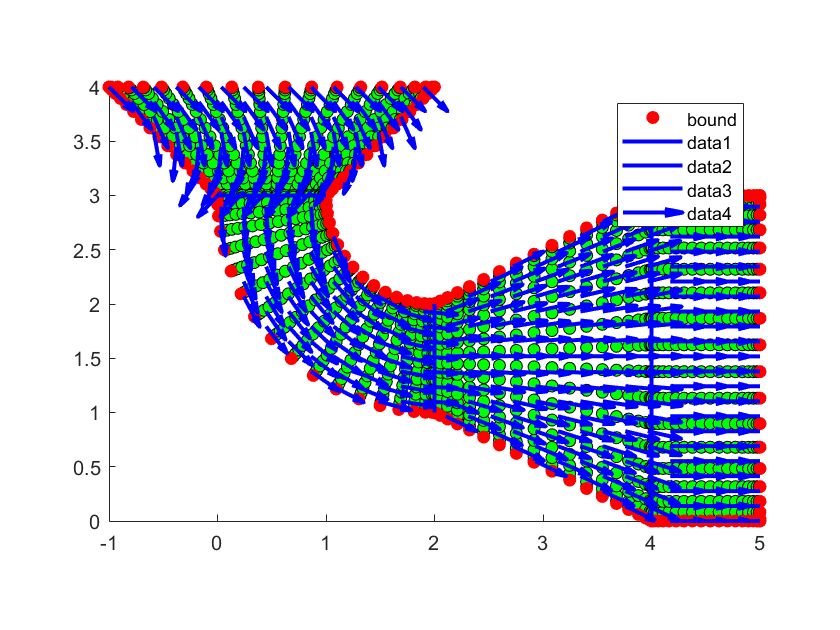
\includegraphics[scale=0.35]{F1.png}
%		\caption{Forward $\rho$ for $a = 0.01$} 
%		\label{F1}
%	\end{figure}

\begin{document}
\section*{MultiShape Theory}
The code library 2DChebClass, introduced in \cite{GoddardPseudospectralCode1}, is a tool for solving PDEs using pseudospectral methods in one and two dimensions on different domains, such as quadrilaterals, wedges and periodic boxes. The aim of this library is to provide a toolbox for solving DDFT in an efficient and user-friendly manner. This includes the automatic set-up of differentiation and convolution matrices, interpolation and integration vectors, as well as domain discretization using pseudospectral methods, identification of boundaries and application of boundary conditions. The library's features are thoroughly explained in \cite{GoddardPseudospectralCode1}.
\\
While the library supports solutions to PDEs on various single shapes, the method is now extended to compute the solution to a PDE on a complex domain, or multishape, which is composed of a number of quadrilaterals and wedges. The philosophy of this multishape code is to use the existing code library \cite{GoddardPseudospectralCode1}, which is designed to efficiently and accurately solve PDEs on individual shapes, to do the same on a multishape with minimal additional effort. 
\\
\\
The solution of a PDE on such a multishape domain is achieved by employing the spectral element method (SEM), by thinking of each of the shapes as the discretization elements of SEM.
This method is similar to the finite element method (FEM). FEM discretizes a domain into elements and computes the solution to a given PDE on each of those elements. Expansions of basis functions are used, which are low order polynomials, for interpolation on an equispaced grid. SEM follows the same philosophy but uses higher order basis functions such as Chebyshev or Lagrange polynomials and Chebyshev-Lobatto points on the interpolation grid on each element, as opposed to an equispaced grid, to avoid the Runge phenomenon. At the intersections between the elements, $C^0$ continuity is enforced. SEM was first introduced by Patera \cite{SEMPatera84} using  Chebyshev polynomials as basis functions and later adapted to Lagrange polynomials by Komatitsch and Vilotte \cite{SEMLagrange98}.
While this method is widely used to solve PDEs in their weak form, in this work the strong form of the PDE is considered, since this aligns best with the existing framework. (?!) Furthermore, instead of just requiring continuity of the solution at the intersection of two elements, the flux (or first derivatives) are also matched. 
\\
\\
In the multishape extension to 2DChebClass, a given PDE is solved on each shape individually, using the preexisting tools in the code library.
This is done simultaneously by stacking the differentiation matrices, integration and interpolation vectors for each shape on top of one another. The initial condition is also given as a stacked vector, containing the information for each shape. This stacking is done using a fixed order of the shapes specified by the user. 
For example, given a function $f$ on a domain $\Omega$ consisting of three shapes labeled $1,2,3$, the solutions on each shape $f_1$, $f_2$ and $f_3$ are stored as:
\begin{align*}
	f_\Omega = [f_1 | f_2 | f_3],
\end{align*}
and similarly, a differentiation matrix $D_\Omega$ is defined as:
\begin{align*}
	D_\Omega = [D_1 | D_2 | D_3],
\end{align*}
where the $D_i$, $i = 1, 2, 3$ are the differentiation matrices on each shape.
\\
The code automatically identifies the intersection boundaries between two shapes when setting up the multishape. The code loops through each face of each shape and compares the points of each face with all faces of the other shapes. It furthermore checks for the possibility that the points of two faces are the same but in reverse order. 
\\
Once the intersections between the neighboring shapes are identified, boundary conditions can be applied. There are currently two options, although the addition of further boundary conditions is straightforward. For a continuous solution on the multishape, both the solution to the PDE and the flux are matched at these intersection boundaries. Alternatively, hard walls between two shapes can be simulated easily, by applying a no-flux boundary condition at that intersection boundary. On boundaries which are on the outside of the multishape, different boundary conditions, such as no-flux and Dirichlet conditions, can be applied in the same way as for single shapes.
\\
\\
When no-flux boundary conditions are applied, a further subtlety is that information about the normal vectors to each outward boundary need to be computed. The existing code library already provides the set of normals for each shape. The multishape extension uses this, alongside the information of which boundaries of each shape are outward boundaries, and which intersect with other shapes, to find the outward normals of the multishape. The only part that needs to be treated with care are the points where two shapes intersect at an outward boundary, since these have two different normals at that intersection point. This is treated in the same way as corners of a single shape, by taking the average of the two normals given by the two faces that meet at the given corner. This is illustrated in Figure \ref{F1} (+++ not yet, why +++)
	\begin{figure}[h]
		\centering
		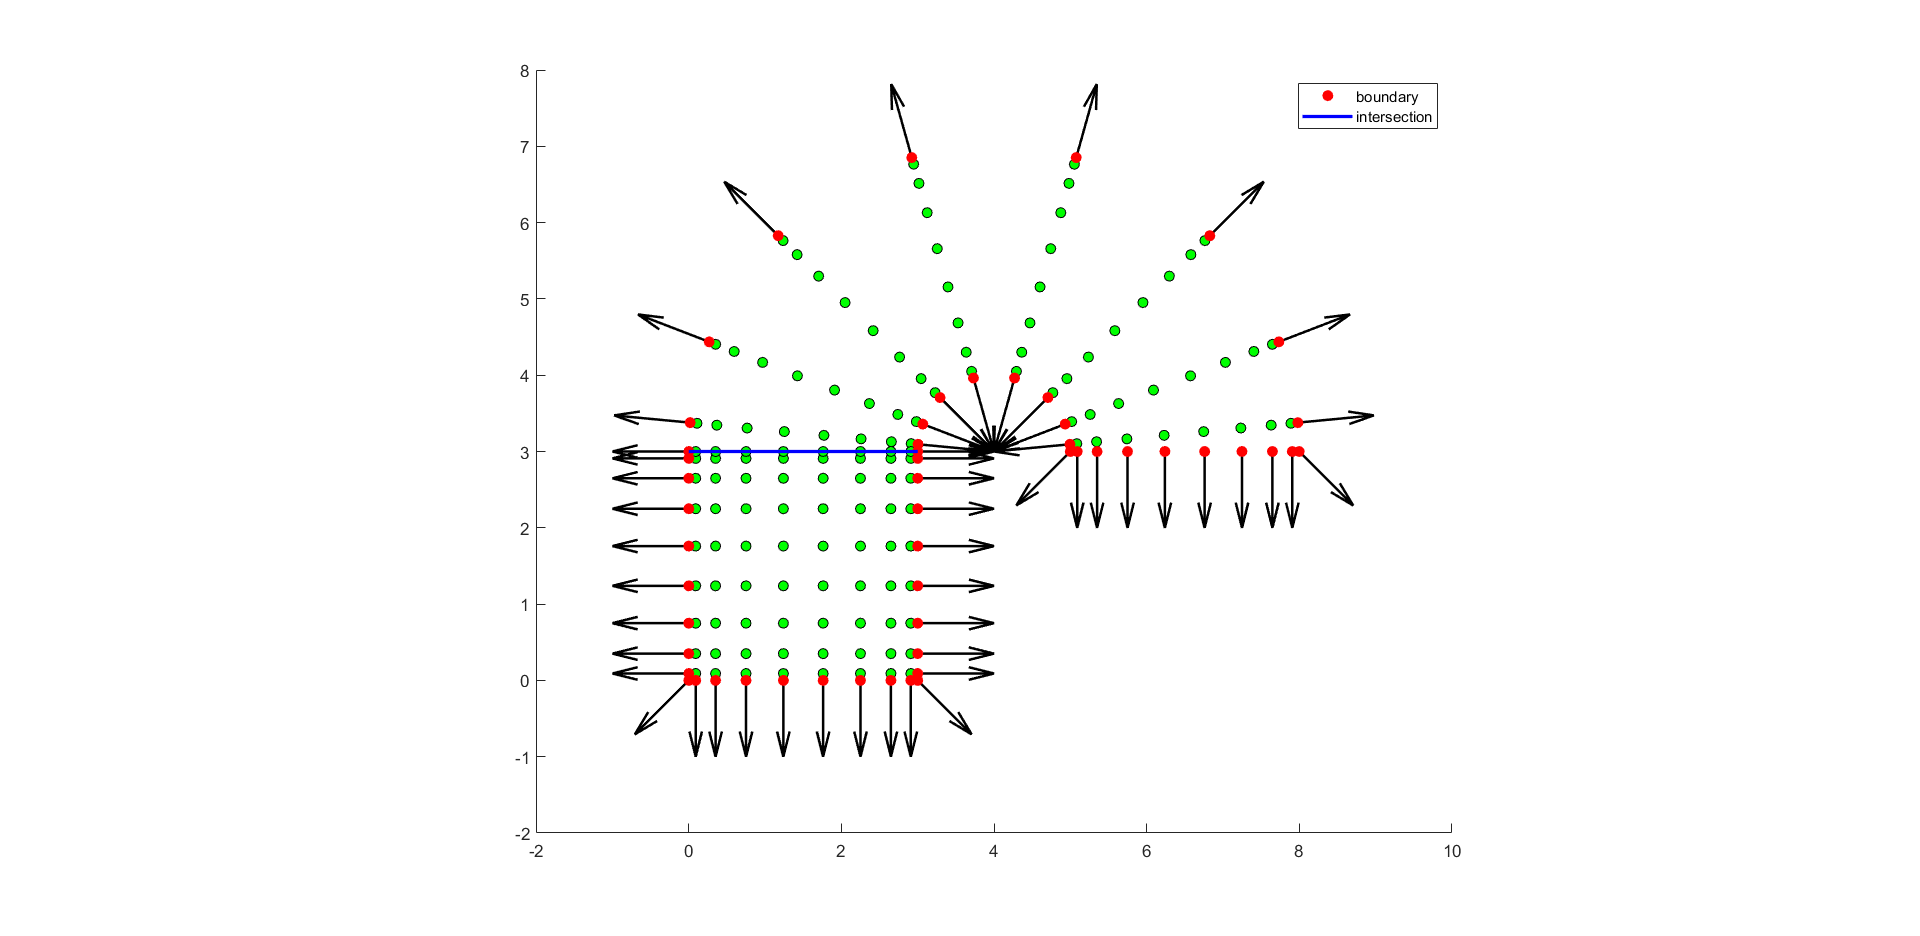
\includegraphics[scale=0.5]{normals.png}
		\caption{Needs fixing} 
		\label{F1}
	\end{figure}
\\
\\
The final aspect to be considered is the convolution matrix, which is needed to compute convolution integrals. It is computed in a similarly straightforward way, but since convolution is a global operation, it is not as simple as stacking the convolution matrices for the individual shapes, as is done for differentiation, integration and interpolation. 
The convolution integral is defined as:
\begin{align*}
	\left(n \star \chi \right) (y) = \int \chi (y - \tilde y) n (\tilde y) d \tilde y.
\end{align*}
As explained in \cite{GoddardPseudospectralCode1} in detail, $\chi$ at $y - \tilde y$ is evaluated for all points in the multishape domain and transformed into a matrix $\text{diag} \left(\chi\right)$. This is integrated, using the stacked integration vector, to result in the convolution matrix, which can then be applied to a density $n$.


\section{Validation Tests}
Several examples are run, using exact solutions, to test whether the multishape code works. This is done using an exact solution to the advection diffusion equation on an infinite domain, so that Dirichlet boundary conditions, matching the value of the exact solution on the boundary of the multishape, can be applied.
The exact solution is:
\begin{align*}
	\rho &= \exp(\alpha t + \beta_1 y_1 + \beta_2 y_2)\\
	\mathbf v &= \left(\beta_1 - \frac{\alpha}{2 \beta_1} + p_1\exp(-\beta_1 y_1) , \beta_2 - \frac{\alpha}{2 \beta_2} + p_2\exp(-\beta_2 y_2) \right),
\end{align*}
where $\beta_1 = -1$, $\beta_2 = 1$, $\alpha = 0.5$, $p_1 = -1$ and $p_2 = 1$.
At first, we compare the exact solution on a box of dimensions $[0,2] \times [0,2] $ with a multishape consisting of two boxes of dimensions $[0,2] \times [0,1]$ and $[0,2] \times [1,2]$, see Figure \ref{F2}. The question is whether the results of the PDE on the box and the dissected box are equal. Each of the shapes are discretized with $N = 20$ points in each spatial direction, which means that the dissected box has more points in total than the original box.
The relative error between the solutions on the two boxes is $1.0034 \times 10^{-10}$. 
When reducing the number of points in the dissected box to $N = 10$ per shape, while keeping $N = 20$ in the single shape box, the relative error in solution is $2.565 \times 10^{-10}$. The solution can be seen in Figure \ref{F3}.

	\begin{figure}[h]
		\centering
		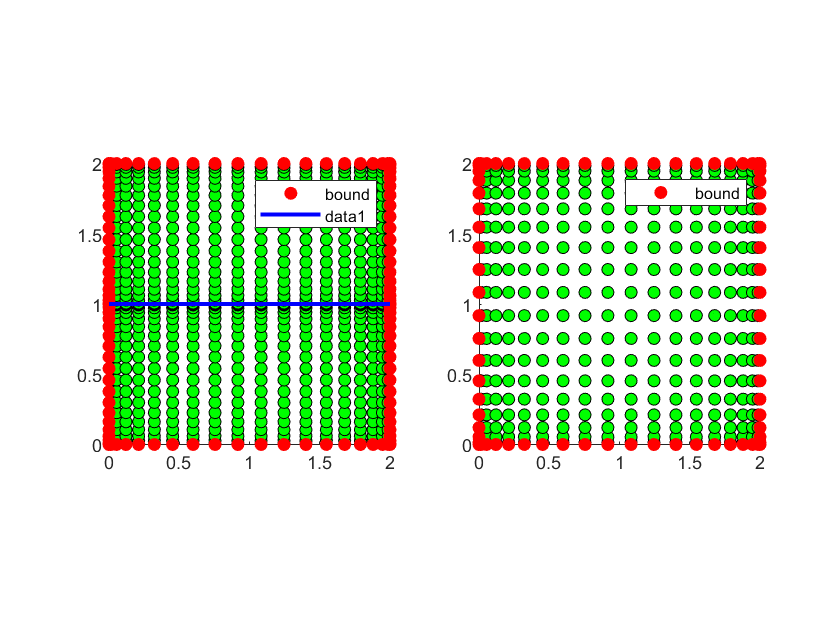
\includegraphics[scale=0.5]{disect1.png}
		\caption{The box and dissected box with $N = 20$} 
		\label{F2}
	\end{figure}

	\begin{figure}[h]
		\centering
		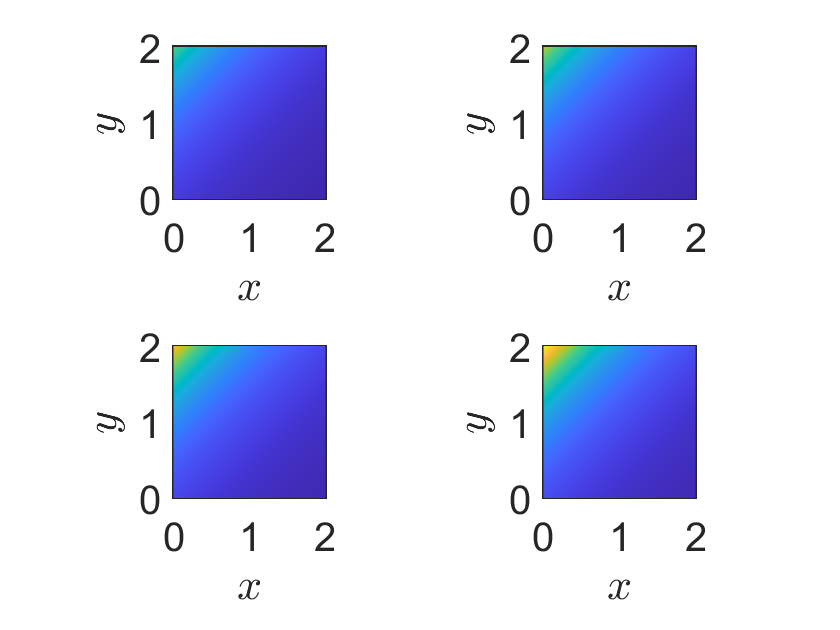
\includegraphics[scale=0.5]{disect2.png}
		\caption{Exact solution on the box} 
		\label{F3}
	\end{figure}
The same test can be done for a wedge. Here, a single wedge and a dissected version are considered, see Figure \ref{F4}. The error in solution between the two approaches with $N = 20$ is $2.0195 \times 10^{-7}$ and with $N = 10$ for each of the two shapes in the disected wedge and $N = 20$ in the full wedge the error is $3.349 \times 10^{-6}$. For $N = 30$ for the shapes in both domains the error is $9.8444 \times 10^{-11}$. This shows that the solution on the wedge is harder to compute accurately and needs more points as compared to the box. The solution can be seen in Figure \ref{F5}.
	\begin{figure}[h]
	\centering
	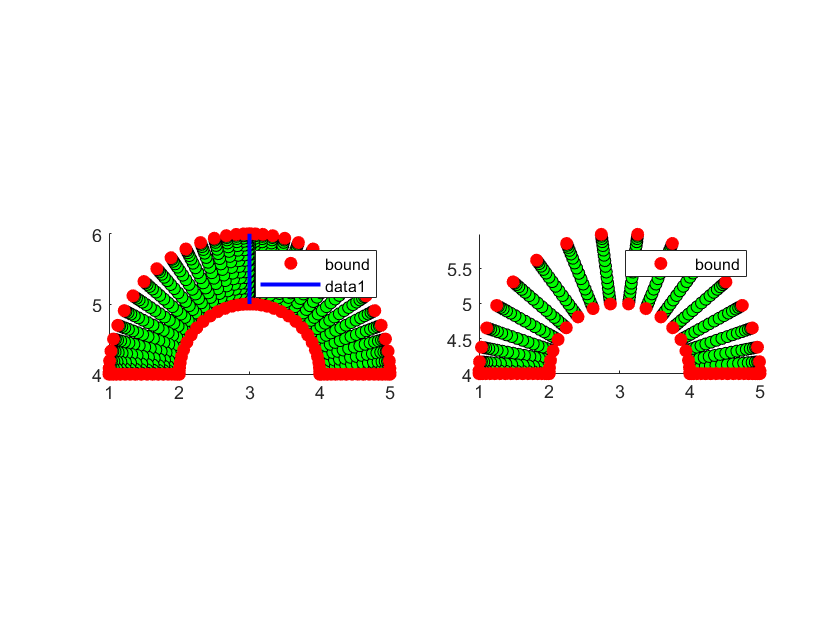
\includegraphics[scale=0.5]{disectW1.png}
	\caption{The wedge and dissected wedge with $N = 20$} 
	\label{F4}
\end{figure}

\begin{figure}[h]
	\centering
	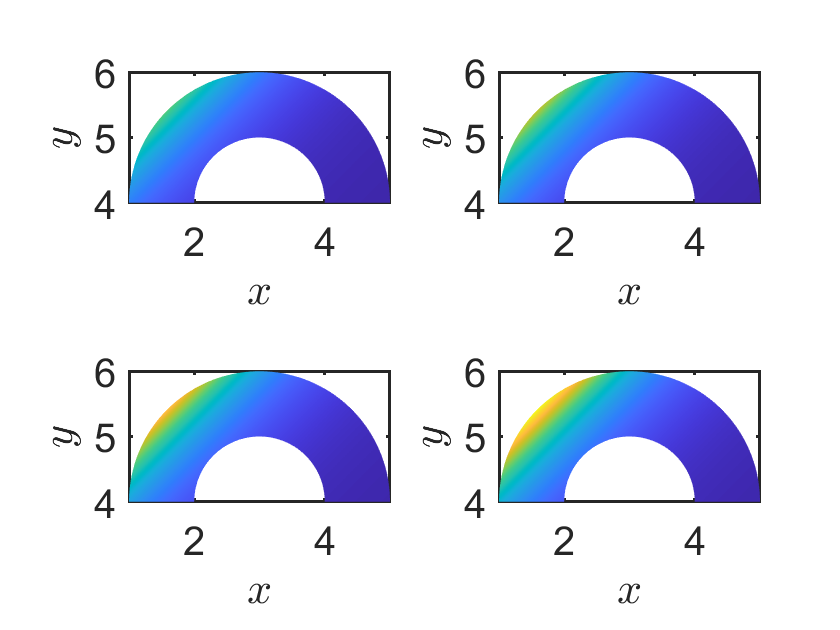
\includegraphics[scale=0.5]{disectW2.png}
	\caption{Exact solution on the wedge} 
	\label{F5}
\end{figure}

Next the advection diffusion equation is solved on a multishape which is composed of four quadrilaterals, see Figure \ref{F6}. The relative error for $N = 20$ on each shape as compared to the exact solution is $2.3321 \times 10^{-9}$. 
\begin{figure}[h]
	\centering
	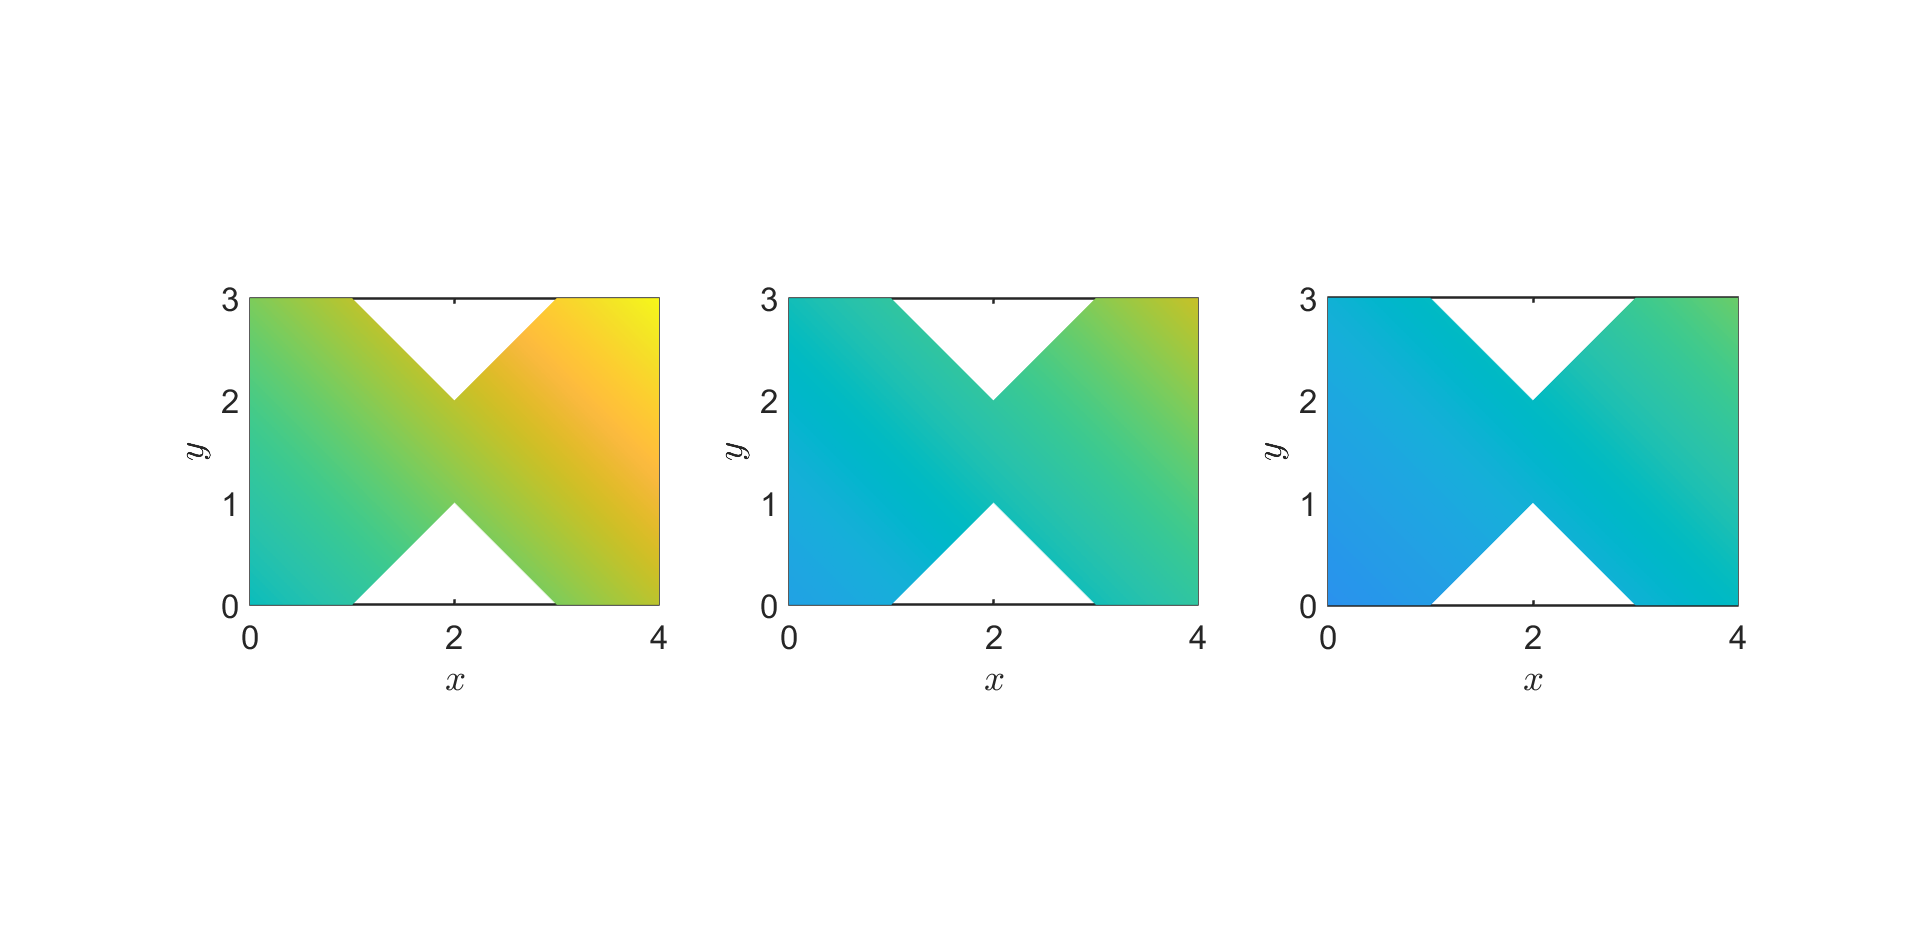
\includegraphics[scale=0.5]{example1.png}
	\caption{Example 1 multishape} 
	\label{F6}
\end{figure}
The same is done for a second example involving a wedge, see Figure \ref{F7}. The relative error to the exact solution is $1.3128 \times 10^{-7}$, when choosing $N= 20$ per shape. We again observe that a larger error is introduced when the multishape includes a wedge as compared to Example 1, which only included quadrilaterals. For $N = 30$ the error decreases to $2.2463 \times 10^{-9}$.

\begin{figure}[h]
	\centering
	\includegraphics[scale=0.5]{example2.png}
	\caption{Example 2 multishape} 
	\label{F7}
\end{figure}


\section{Forward Problems on multishapes}

The first example is solving an advection diffusion problem on a multishape consisting of two quadrilaterals and two wedges, with constant velocity of strength ten. The initial condition for this problem is:
 \begin{align*}
 	\rho_0 = \exp( -2(y_1 -0.5)^2 - 2 (y_2 + 1)^2).
 \end{align*}
The result, evaluated for $N= 20$ on each shape, can be seen in Figure \ref{F8}.

\begin{figure}[h]
	\centering
	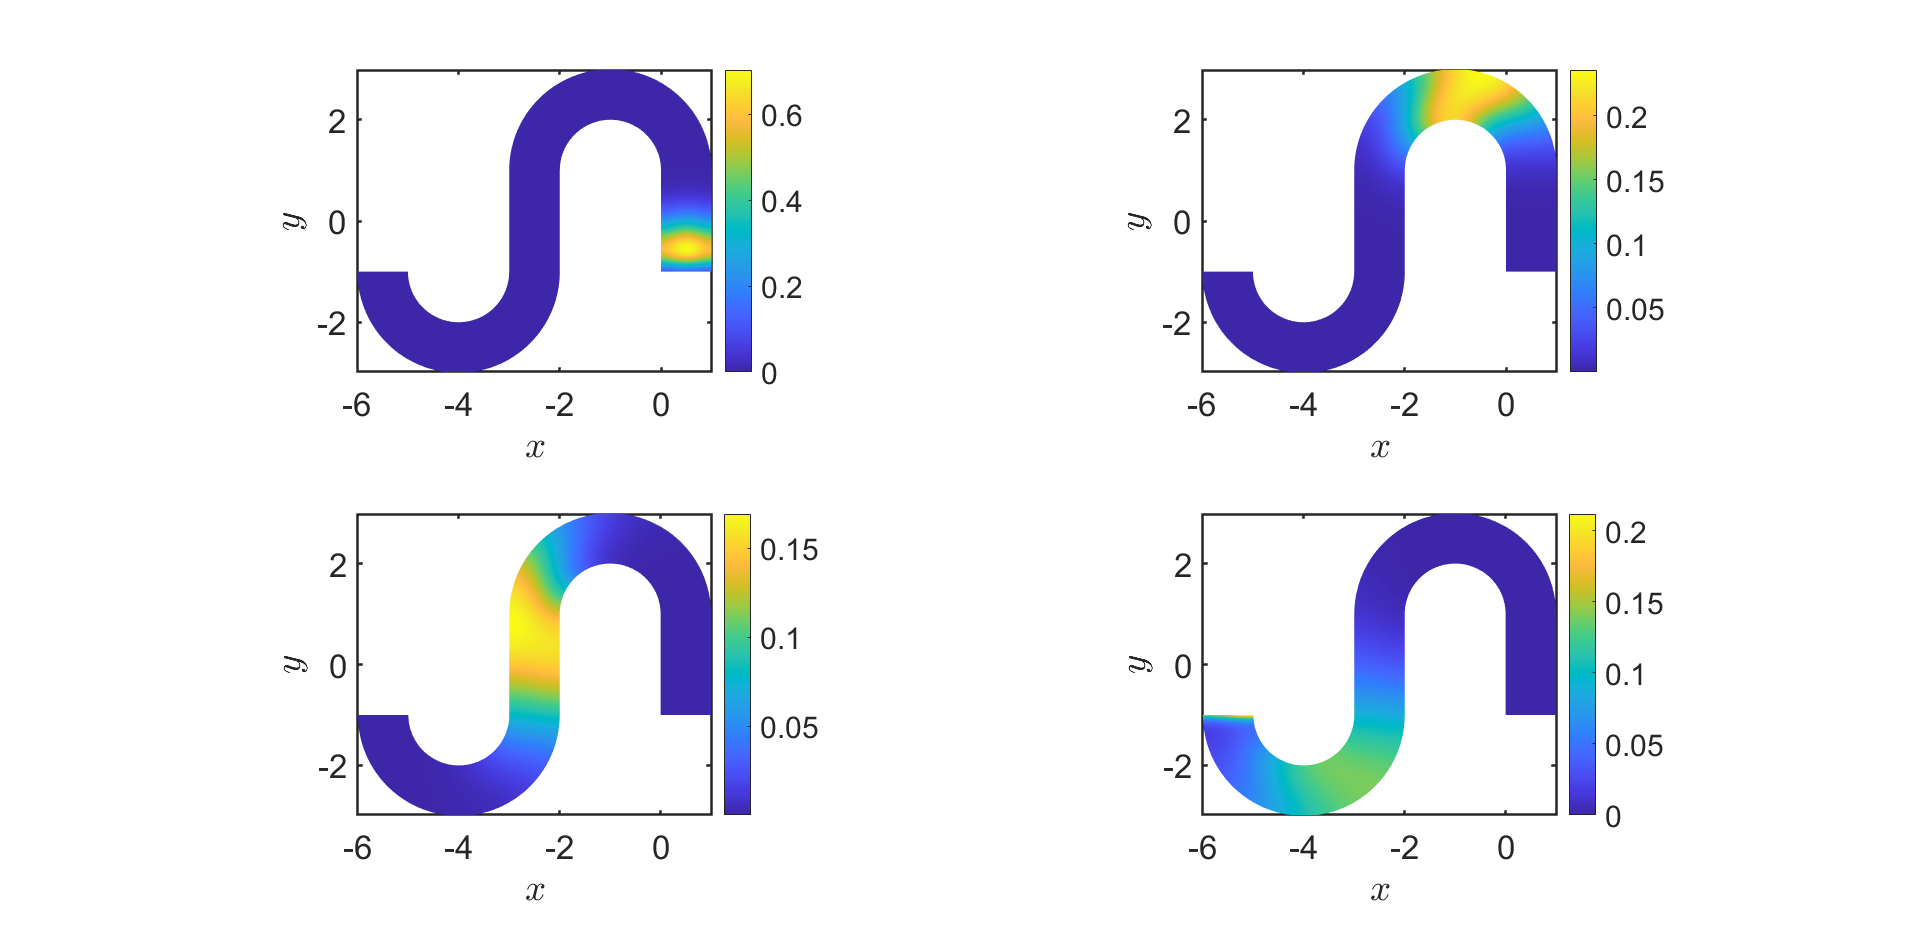
\includegraphics[scale=0.5]{ex1.png}
	\caption{Forward Problem 1}
	\label{F8}
\end{figure}

In a second example, the velocity is of strength $5$ and the initial condition is:
 \begin{align*}
	\rho_0 = \exp( -2(y_1 -0.5)^2 - 2 (y_2 - 1.5)^2).
\end{align*}
The result, which is computed on a multishape made up of four quadrilaterals into a channel, can be seen in Figure \ref{F9}.

\begin{figure}[h]
	\centering
	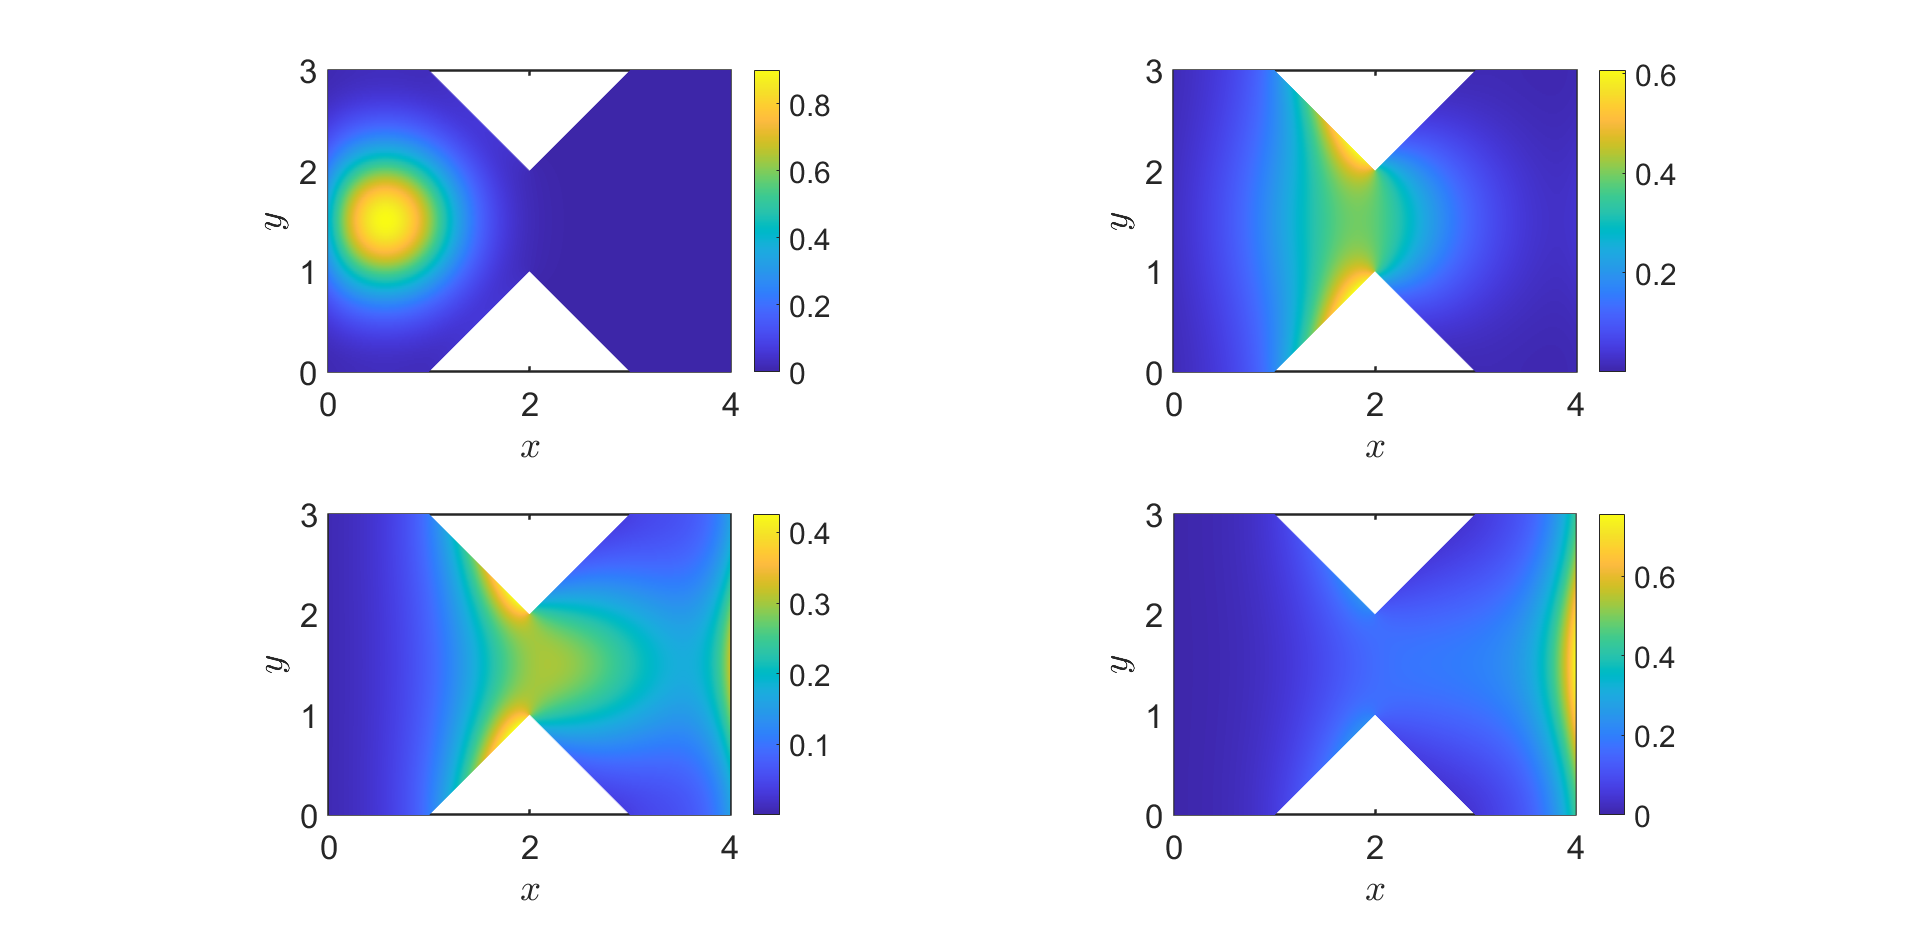
\includegraphics[scale=0.5]{ex2.png}
	\caption{Forward Problem 2}
	\label{F9}
\end{figure}








\pagebreak	
\bibliography{GeneralBib}
\bibliographystyle{unsrt}
\end{document}	
    In this section the advantages and disadvantages of pseudospectral methods over finite element methods (FEM) and finite difference methods (FDM) are discussed, compare to \cite{Boyd1}.
The main difference between pseudospectral methods (PSM) and the other two methods is that PSM uses global basis functions on all Chebyshev points, while FEM uses local basis functions and FDM uses local, low order polynomials.
\\
Finite difference methods use overlapping sequences of polynomials to approximate the solution of the problem. They are easy to implement and less costly per degree of freedom. However, they are also less accurate than PSM.
\\
The basis functions used in FEM methods are generally of fixed, low degree and more accuracy is achieved through refinement of the elements; either in the whole domain or in regions where the problem is more difficult to solve.
In comparison, the global basis function used in PSM are generally of higher degree than the ones in FEM. Furthermore, in order to refine the method, the degree of the polynomial can be increased.
\\
In general, FEM results in large sparse matrix systems, which in many cases can be solved by exploiting their structure. It is also easily applied to complex domains, due to the shape of the elements.
However, the disadvantage of FEM is low accuracy of solutions, due to the low degree of the polynomial basis functions. Furthermore, the sparsity property of the matrix systems is compromised when the PDEs involve nonlocal terms. Therefore, PSM are advantageous in this type of problems, since small dense matrices are utilized. 
 As discussed in \cite{FEMIntegroPaper}, an adaptive FEM method can be used to solve an integro-differential PDE-constrained optimal control problem. However, the accuracy achieved is mainly of order $O(10^{-2})$ and maximal $O(10^{-4})$, for a two dimensional problem with $N$ nodes, where $N$ is between $N=3549$ and $50421$. The time step is $dt=0.05$. Furthermore, Dirichlet boundary conditions are used, which avoids applying more realistic no-flux boundary conditions. These no-flux boundary conditions are difficult to apply in the FEM context, because they are nonlocal as well. Within the existing code framework \cite{GoddardPseudospectralCode1}, these boundary conditions are straightforward to apply.
The disadvantages of PSM are that they are more computationally expensive and the domain is required to be smooth.
However, as discussed in \cite{Boyd1}, if the accuracy of PSM with $N=10$ is to be achieved by FEM or FDM, a 10th order method has to be chosen with an error of $O(h^{10})$.
All in all, PSM is the best method for solving PDE-contrained optimization problems involving integro-PDEs.
    
    
    
    
    
	\section{PDE-Constrained Optimization}
	
	\subsection{General PDECO Stuff}
		\begin{itemize}
			\item General Intro to the class of problems and a general problem setup
			\item Link to other areas?
			\item Literature review of Mean-Field PDECO and link between the two fields.
			\item Here may be a good point to go into the mean-field convergence stuf of the microscopic OCP to ours a little more.
		\end{itemize}
	The aim of this project is to work towards using the particle model derived in the previous section to describe an industrial process and optimize this process with minimal cost involved.
It is of interest to achieve a particle distribution $\hat{\rho}$ in some time over some domain $\Omega$.  
In the context of PDE-constrained optimization, the aim is to minimize the distance between a state variable $\rho$ and a desired state $\hat\rho$, in some norm, while also minimizing the cost involved in reaching the desired state. This minimization is constrained by the underlying physics of the particle system. The PDE describing the particle dynamics is called the state equation.
\newline
Achieving the desired state $\hat\rho$ as close as possible can be of interest either for all times, as in this report, or only at some times, such as the final time $T$. In order to achieve $\hat \rho$, the particle distribution $\rho$ can be controlled through a so-called control variable, denoted by $u$. The control can be applied in various ways, which is dependent on the application. Since the background flow influences the particle distribution $\rho$, $\hat\rho$ can try to be reached by changing the flow field. Then the flow field is the control $u$. Alternatively, $u$ could represent the temperature or the geometry of the boundaries of the bath. Moreover, $u$ could be a parameter in the body force or in the particle interaction term, influencing the particle distribution through the forces involved. Note that $u$ cannot always influence the system enough to reach the desired state $\hat \rho$. This highly depends on the choice of $\hat \rho$, the physics of the problem and on the choice of the parameter $\beta$, which is discussed below.
Since controlling $\rho$ requires energy, $u$ can be thought of as the cost involved in reaching $\hat\rho$. 
\\ 
The weight of the control is determined by the so-called regularization parameter, $\beta$. If $\beta$ is small, the desired state will be reached, however, at a high cost. If $\beta$ is large, the control will be minimized, but the desired state might not be reached. The choice of $\beta$ depends on the application involved. It is generally of interest to find a range of $\beta$ values, for which the solution to the optimization problem is robust. 
The PDE-constrained optimization problem of interest in this report is of the form:
\begin{align} \label{sysPDEconOpti1}
&\min_{\rho,\mathbf{w}} \quad \frac{1}{2}\norm{\rho- \hat{\rho}}_{L^2}^2 + \frac{\beta}{2} \norm{\mathbf{w}}_{L^2}^2,\\
\notag\\
&\textbf{subject to:}\notag\\ 
&\partial_t \rho =\nabla^2 \rho - \nabla \cdot (\rho \mathbf{w}) + \nabla \cdot (\rho \nabla V_{ext}) \quad \text{in} \quad \Omega,\notag\\
\notag\\
&\dfrac{\partial \rho}{\partial {n}} - \rho \mathbf{w} \cdot \mathbf{n} + \rho \dfrac{\partial V_{ext}}{\partial {n}}  =0 \quad \text{on} \quad \partial \Omega,\notag \\
& \rho = \rho_0 \quad \text{at} \quad t=0,  \notag
\end{align}
where the state equation is a simplified version of (\ref{sysParticleModel1}), which neglects the particle interaction term.
Note that the norms are the $L^2$ norms with respect to $\Omega$ and time. Other norms could be used, depending on the type of application. In the following it is assumed, as described in \cite{TroeltzschFredi2010OCoP}, that $\rho \in H^1$ and $\mathbf{w} \in L^2$.
In order to solve this optimization problem, continuous optimality conditions can be derived, which can then be discretized and solved numerically. This is known as the optimize-then-discretize approach.
Another approach, discretize-then-optimize, would be to first discretize (\ref{sysPDEconOpti1}) and then derive the discrete optimality conditions that need to be solved.
A good introduction to PDE-constrained optimization, can be found in \cite{PearsonThesis} and a more detailed introduction to numerical PDE-constrained optimization is provided in \cite{DeLosReyesOptimization}. Both of these texts provided the basis for the above discussion.

\subsection{Deriving First-Order Optimality Conditions}
Employing the  optimize-then-discretize approach, the continuous first order optimality conditions are derived using a Lagrangian approach. These are necessary optimality conditions, however, the sufficient second-order optimality conditions would be needed to ensure that the stationary points found via the first-order optimality conditions are indeed the minima of the problem. Sufficient optimality conditions are not part of this report but can be found, along the underlying theory of the approach employed in this section, in \cite{DeLosReyesOptimization} and \cite{TroeltzschFredi2010OCoP}. The derivation of the first-order optimality system follows closely the presentation in \cite{TroeltzschFredi2010OCoP}.  
The PDE-constrained optimization problem (\ref{sysPDEconOpti1}) in Lagrangian form is:
\begin{align*}
\mathcal{L}(\rho,\mathbf{w}, p_\Omega, p_{\partial \Omega}) &= \frac{1}{2} \norm{\rho- \hat{\rho}}_{L^2(\Omega,t)}^2+ \frac{\beta}{2} \norm{\mathbf{w}}_{L^2(\Omega,t)}^2 \\
&+  \int_0^T \int_\Omega\bigg( \partial_t \rho - \nabla^2 \rho + \nabla \cdot (\rho \mathbf{w}) - \nabla \cdot (\rho \nabla V_{ext}) \bigg) p_\Omega dr dt  \\ 
&+ \int_0^T \int_{\partial \Omega}  \bigg(\dfrac{\partial \rho}{\partial {n}} - \rho \mathbf{w} \cdot \mathbf{n} + \rho \dfrac{\partial V_{ext}}{\partial {n}}\bigg) p_{\partial \Omega} dr dt , 
\end{align*}
where $p_\Omega$ and $p_{\partial \Omega}$ are the Lagrange multipliers of the problem, relating to the interior and the boundary of $\Omega$, respectively. The Lagrange multiplier $p_\Omega \in L^2$ is called the adjoint variable in the resulting system of equations.
Writing the $L^2$ norms explicitly gives:
\begin{align} \label{sysLagrangian1}
\mathcal{L}(\rho,\mathbf{w}, p_\Omega, p_{\partial \Omega}) &= \frac{1}{2}\int_0^T\int_\Omega  (\rho- \hat{\rho})^2 dr dt  + \frac{\beta}{2} \int_0^T \int_\Omega \mathbf{w}^2 dr dt  \\
&+ \int_0^T \int_\Omega \bigg( \partial_t \rho - \nabla^2 \rho + \nabla \cdot (\rho \mathbf{w}) - \nabla \cdot (\rho \nabla V_{ext}) \bigg) p_\Omega dr dt \notag \\ 
&+\int_0^T  \int_{\partial \Omega}  \bigg(\dfrac{\partial \rho}{\partial {n}} - \rho \mathbf{w} \cdot \mathbf{n} + \rho \dfrac{\partial V_{ext}}{\partial {n}}\bigg) p_{\partial \Omega} dr dt  \notag.
\end{align}
It is beneficial to rewrite the part of (\ref{sysLagrangian1}) that comes from the state equation, in order to simplify further computations.
The term of interest is:
\begin{align*}
 &\int_0^T \int_\Omega \bigg( \partial_t \rho - \nabla^2 \rho + \nabla \cdot (\rho \mathbf{w}) - \nabla \cdot (\rho \nabla V_{ext}) \bigg) p_\Omega dr dt \\
 &=   \int_0^T \int_\Omega   p_\Omega \partial_t \rho dr dt -\int_0^T  \int_\Omega  p_\Omega \nabla^2 \rho dr dt  + \int_0^T \int_\Omega \nabla \cdot (\rho \mathbf{w}) p_\Omega dr dt -\int_0^T \int_\Omega \nabla \cdot (\rho \nabla V_{ext})p_\Omega dr dt \\
 &:= I_1 + I_2 + I_3 + I_4. 
\end{align*}
Each of the defined integrals is considered in turn.
The first integral contains the time derivative of $\rho$. Integration by parts is applied to get:
\begin{align*}
I_1&=\int_0^T \int_\Omega  p_\Omega \partial_t \rho dr dt  = \bigg[ \int_\Omega \rho p_\Omega dr \bigg]_0^T - \int_0^T \int_\Omega \rho\partial_t  p_\Omega dr dt\\
&= \int_\Omega (\rho(T) p_\Omega(T) -\rho_0 p_\Omega(0))dr  - \int_0^T \int_\Omega \rho\partial_t  p_\Omega dr dt .
\end{align*}
In order to rewrite the second integral, integration by parts is applied twice as follows:
\begin{align*}
I_2&=  \int_0^T \int_\Omega p_\Omega \nabla^2 \rho dr dt  
=\int_0^T \int_{\partial \Omega}  p_\Omega \frac{\partial \rho}{\partial {n}} dr dt  -\int_0^T \int_\Omega  \nabla \rho \cdot \nabla p_\Omega dr dt \\
&=\int_0^T \int_{\partial \Omega}  p_\Omega \frac{\partial \rho}{\partial n} dr dt - \int_0^T \int_{\partial \Omega}  \rho \frac{\partial p_\Omega }{\partial {n}} dr dt   +\int_0^T \int_\Omega \rho \nabla^2 p_\Omega dr dt .
\end{align*} 
The third integral is rewritten using similar arguments:
\begin{align*}
I_3 = \int_0^T \int_\Omega \nabla \cdot (\rho w) p_\Omega dr dt = \int_0^T  \int_{\partial \Omega}  p_\Omega \rho w \cdot n dr dt  - \int_0^T \int_\Omega \rho \nabla p_\Omega \cdot w dr dt.
\end{align*}
The final integral is rewritten as follows:
\begin{align*}
I_4 &=\int_0^T \int_\Omega \nabla \cdot (\rho \nabla V_{ext})p_\Omega dr dt=\int_0^T \int_\Omega \nabla \cdot (\rho \nabla V_{ext}p_\Omega) dr dt  - \int_0^T \int_\Omega  \rho \nabla p_\Omega\cdot \nabla V_{ext} dr dt\\
&= \int_0^T \int_{\partial\Omega}  \rho p_\Omega \frac{\partial V_{ext}}{\partial n} dr dt - \int_0^T \int_\Omega  \rho \nabla p_\Omega\cdot \nabla V_{ext} dr dt,
\end{align*}
where the Divergence Theorem is used to derive the final result.
Substituting the four rewritten integrals back into (\ref{sysLagrangian1}) results in:
\begin{align*}
\mathcal{L}(\rho,\mathbf{w}, p_\Omega, p_{\partial \Omega}) &= \frac{1}{2}\int_0^T \int_\Omega  (\rho- \hat{\rho})^2 dr dt+ \frac{\beta}{2}\int_0^T \int_\Omega  \mathbf{w}^2 dr dt   
+ \int_\Omega (\rho(T) p_\Omega(T) -\rho_0 p_\Omega(0))dr \\ \notag 
&- \int_0^T\int_\Omega \rho\partial_t  p_\Omega dr dt - \int_0^T \int_{\partial \Omega}  p_\Omega \frac{\partial \rho}{\partial n} dr dt + \int_0^T \int_{\partial \Omega}  \rho \frac{\partial p_\Omega }{\partial n} dr dt  - \int_0^T \int_\Omega \rho \nabla^2 p_\Omega dr dt  \notag \\
&+ \int_0^T \int_{\partial \Omega} p_\Omega \rho \mathbf{w} \cdot \mathbf{n} dr dt  - \int_0^T \int_\Omega  \rho \nabla p_\Omega \cdot \mathbf{w} dr dt \notag 
- \int_0^T \int_{\partial\Omega}  \rho p_\Omega \frac{\partial V_{ext}}{\partial n} dr dt   \notag \\
& +\int_0^T \int_\Omega  \rho \nabla p_\Omega\cdot \nabla V_{ext} dr dt  + \int_0^T \int_{\partial \Omega}  \bigg(\dfrac{\partial \rho}{\partial n} - \rho \mathbf{w} \cdot \mathbf{n} + \rho \dfrac{\partial V_{ext}}{\partial n}\bigg) p_{\partial \Omega} dr  dt\notag.
\end{align*}
Sorting the terms by whether they are interior or boundary terms and grouping them gives: 
\begin{align} \label{sysLagrangian2}
&\mathcal{L}(\rho,\mathbf{w}, p_\Omega, p_{\partial \Omega}) =\int_\Omega (\rho(T) p_\Omega(T) -\rho_0 p_\Omega(0))dr \\
&+ \int_0^T \int_\Omega \bigg( \frac{1}{2}(\rho- \hat{\rho})^2  + \frac{\beta}{2} \mathbf{w}^2 - \rho\partial_t  p_\Omega  - \rho \nabla p_\Omega \cdot \mathbf{w}   \notag 
- \rho \nabla^2 p_\Omega +  \rho \nabla p_\Omega\cdot \nabla V_{ext} \bigg)dr dt  \\
& + \int_0^T \int_{\partial \Omega}  \bigg( \rho \frac{\partial p_\Omega }{\partial n}  -  \rho p_\Omega \frac{\partial V_{ext}}{\partial n} 
- p_\Omega \frac{\partial \rho}{\partial n} 
+ p_\Omega \rho \mathbf{w} \cdot \mathbf{n} \notag 
+ p_{\partial \Omega} \dfrac{\partial \rho}{\partial n} - \rho p_{\partial \Omega} \mathbf{w} \cdot \mathbf{n} + \rho p_{\partial \Omega} \dfrac{\partial V_{ext}}{\partial n}  \bigg) dr dt  \notag.
\end{align}

In order to derive the first-order optimality conditions for the optimization problem, the Fr\'echet derivatives of $\mathcal{L}$ with respect to all variables $\rho, w, p_\Omega, p_{\partial \Omega}$ have to be taken. The system of equations that results from setting these first derivatives to zero are called first-order optimality conditions. The resulting equations are called the adjoint equation, the gradient equation and the forward problem. The latter is equivalent to the state equation.

\subsubsection{Fr\'echet Differentiation}
In the derivation of the optimality conditions, Fr\'echet derivatives of the Lagrangian have to be taken. In order to do so, the notions of derivatives needed in this context are introduced in this section.

The following definitions are taken from \cite{DeLosReyesOptimization} and \cite{FrechetProductrule1}.
Throughout this section, let $U,V$ and $Z$ be real Banach spaces.
\theoremstyle{definition}
\begin{definition}\cite{DeLosReyesOptimization}
If, for given elements $ u,h \in U$, the limit
\begin{align*}
\delta F(u)(h) := \lim_{t\to 0^+} \frac{1}{t} \bigg( F(u+th) - F(u) \bigg)
\end{align*}
exists, then $\delta F(u)(h)$ is called the \emph{directional derivative} of $F$ at $u$ in direction $h$. If this limit exists for all $h \in U$, then $F$ is called directionally differentiable at $u$.
\end{definition}
\theoremstyle{definition}
\begin{definition}\cite{DeLosReyesOptimization}
	If, for some $ u \in U$ and all $h \in U$ the limit
	\begin{align*}
	\delta F(u)(h) := \lim_{t\to 0} \frac{1}{t} \bigg( F(u+th) - F(u) \bigg)
	\end{align*}
	exists and $\delta F(u)(h)$ is a continuous mapping from $U$ to $V$, then $\delta F(u)$ is denoted by $F'(u)$ and is called the G\^{a}teaux derivative of $F$ at $u$, and $F$ is called \emph{G\^{a}teaux differentiable} at $u$.
\end{definition}

\theoremstyle{definition}
\begin{definition}\cite{DeLosReyesOptimization}
If $F$ is G\^{a}teaux differentiable at $u \in U$, and satisfies in addition that
\begin{align*}
\lim_{\norm{h}_U \to 0} \frac{\norm{F(u+h)-F(u) -F'(u)h}_V}{\norm{h}_U}=0,
\end{align*}
then $F'(u)$ is called the Fr\'echet derivative of $F$ at $u$ and $F$ is called \emph{Fr\'echet differentiable}.
\end{definition}

\theoremstyle{definition}
\begin{definition}\cite{DeLosReyesOptimization} \emph{Chain Rule}\\
Let $F:U\to V$ and $G:V \to Z$ be Fr\'echet differentiable at $u$ and $F(u)$, respectively. Then
\begin{align*}
E(u)=G(F(u))
\end{align*}
is also Fr\'echet differentiable and its derivative is given by:
\begin{align*}
E'(u)=G'(F(u))F'(u).
\end{align*} 
\end{definition}

\theoremstyle{definition}
\begin{definition}\cite{FrechetProductrule1} \emph{Product Rule}\\
Let $U$ and $V$ be Banach spaces, let $\mathcal{U}$ be an open subset of $U$, and let $F: \mathcal{U} \to \mathbf{R}$ and $G: \mathcal{U} \to V$ be functions. If both $F$ and $G$ are differentiable at $u \in \mathcal{U}$, then $FG$ is differentiable at $u$ and 
\begin{align*}
(FG)'(u) = F(u)G'(u)+G(u)F'(u).
\end{align*}
\end{definition}

\subsubsection{Deriving the Adjoint Equation} \label{secOptimalityAdjoint1}
The adjoint equation is found by calculating the Fr\'echet derivative of the Lagrangian (\ref{sysLagrangian2}) with respect to the state variable and setting it equal to zero.
The derivative with respect to $\rho$ is:
\begin{align*}
&\mathcal{L}_\rho (\rho,\mathbf{w}, p_\Omega, p_{\partial \Omega}) h =\int_\Omega h(T) p_\Omega(T) dr\\
&+ \int_0^T\int_\Omega  \bigg( (\rho- \hat{\rho})h   - h\partial_t  p_\Omega  - h\nabla p_\Omega \cdot  \mathbf{w} - h \nabla^2 p_\Omega \notag 
 +  h \nabla p_\Omega\cdot \nabla V_{ext} \bigg)dr dt  \\
& + \int_0^T  \int_{\partial \Omega}  \bigg(h \frac{\partial p_\Omega }{\partial n}  -  h p_\Omega \frac{\partial V_{ext}}{\partial n} 
- p_\Omega \frac{\partial h}{\partial n} 
+ p_\Omega h \mathbf{w} \cdot \mathbf{n} \notag 
+ p_{\partial \Omega} \dfrac{\partial h}{\partial n} - h p_{\partial \Omega} \mathbf{w} \cdot \mathbf{n} + h p_{\partial \Omega} \dfrac{\partial V_{ext}}{\partial n}  \bigg) dr dt  \notag\\
&=\int_\Omega h(T) p_\Omega(T) dr + \int_0^T\int_\Omega  \bigg( (\rho- \hat{\rho})   - \partial_t  p_\Omega  - \nabla p_\Omega \cdot \mathbf{w}  - \nabla^2 p_\Omega \notag 
 +  \nabla p_\Omega\cdot \nabla V_{ext} \bigg)h dr dt \\
& + \int_0^T\int_{\partial \Omega}   \bigg(
\bigg(\frac{\partial p_\Omega }{\partial n} + p_\Omega  \mathbf{w} \cdot \mathbf{n} - p_{\partial \Omega} \mathbf{w} \cdot \mathbf{n} +  p_{\partial \Omega} \dfrac{\partial V_{ext}}{\partial n} - p_\Omega \frac{\partial V_{ext}}{\partial n} \bigg)h
+ \bigg( p_{\partial \Omega}- p_\Omega \bigg) \frac{\partial h}{\partial n} \bigg) dr dt \notag,
\end{align*}
where $h \in L^2$ belongs to the same space as $\rho$ and can be thought of as the direction of differentiation.
The initial condition for $\rho$, $\rho_0$, vanishes from the derivative of $\mathcal{L}$, because $h$ satisfies $h(r,0)=0$. As discussed in \cite{TroeltzschFredi2010OCoP}, this is because the variational inequality $\mathcal{L}_\rho(\tilde \rho, \mathbf{\tilde w},p_\Omega, p_{\partial\Omega})(\rho -\tilde\rho)\geq 0$ has to be satisfied for all admissible $\rho$, in order for $\tilde \rho$ and $\mathbf{\tilde w}$ to be the minimum of the problem.
If $h:=\rho-\tilde \rho$, then $h(r,0)=0$ and furthermore, $-h$ is also an admissible choice of function. Therefore, the variational inequality becomes the equality $\mathcal{L}_\rho(\tilde \rho,\mathbf{\tilde w},p_\Omega, p_{\partial\Omega})h= 0$, for $h$ sufficiently smooth, with $h(r,0)=0$. 

Setting $\mathcal{L}_\rho (\rho,\mathbf{w}, p_\Omega, p_{\partial \Omega}) h =0$, in order to find the adjoint equation, gives:
\begin{align} \label{eqnLagrRhoDeriv}
&\mathcal{L}_\rho (\rho,\mathbf{w}, p_\Omega, p_{\partial \Omega}) h =\int_\Omega h(T) p_\Omega(T) dr\\
&+ \int_0^T \int_\Omega \bigg( (\rho- \hat{\rho})   - \partial_t  p_\Omega  - \nabla p_\Omega \cdot \mathbf{w}  - \nabla^2 p_\Omega \notag 
  +  \nabla p_\Omega\cdot \nabla V_{ext} \bigg)h dr dt  \notag \\
& +  \int_0^T\int_{\partial \Omega}  \bigg(
\bigg(\frac{\partial p_\Omega }{\partial n} + p_\Omega  \mathbf{w} \cdot \mathbf{n} - p_{\partial \Omega} \mathbf{w} \cdot \mathbf{n} +  p_{\partial \Omega} \dfrac{\partial V_{ext}}{\partial n} - p_\Omega \frac{\partial V_{ext}}{\partial n} \bigg)h \notag+ \bigg( p_{\partial \Omega}- p_\Omega \bigg) \frac{\partial h}{\partial n} \bigg) dr dt =0. \notag
\end{align}
The first step is to restrict the choice of $h$ as much as possible. That is choosing $h \in C_0^\infty(\Omega)$, such that: 
\begin{align}\label{condHChoice1}
h(T)&=0 \quad \text{in} \quad \Omega, \\
h&=0 \quad \text{on} \quad \partial \Omega, \notag \\
\frac{\partial h}{\partial n}&=0 \quad \text{on} \quad \partial \Omega, \notag
\end{align}
as discussed in \cite{TroeltzschFredi2010OCoP}.
With this choice of $h$, (\ref{eqnLagrRhoDeriv}) reduces to:
\begin{align}\label{eqnOptiAdjRho1}
\mathcal{L}_\rho (\rho,\mathbf{w}, p_\Omega, p_{\partial \Omega}) h 
 &= \int_0^T \int_\Omega  \bigg( (\rho- \hat{\rho})   - \partial_t  p_\Omega  - \nabla p_\Omega \cdot \mathbf{w}  - \nabla^2 p_\Omega 
 +  \nabla p_\Omega\cdot \nabla V_{ext} \bigg)h dr dt  \notag \\
&=0.
\end{align}
Since this equation has to hold for all $h$ satisfying (\ref{condHChoice1}) and, as discussed in \cite{TroeltzschFredi2010OCoP}, $C_0^\infty(\Omega)$ is dense in $L^2(\Omega)$, it can be concluded that:
\begin{align*}
(\rho- \hat{\rho})   - \partial_t  p_\Omega  - \nabla p_\Omega \cdot \mathbf{w}  - \nabla^2 p_\Omega 
  +  \nabla p_\Omega\cdot \nabla V_{ext} =0.
\end{align*}
The adjoint equation is then
\begin{align*}
 - \partial_t  p_\Omega  - \nabla p_\Omega \cdot \mathbf{w}  - \nabla^2 p_\Omega 
+  \nabla p_\Omega\cdot \nabla V_{ext} =-(\rho- \hat{\rho}) . 
\end{align*}
Now it is of interest to relax the conditions on $h$, to derive the results at the boundary $\partial \Omega$ and at the final time $T$.
First, the case where $h(T) \neq 0$ is considered, so that $h \in C^1(\Omega)$. The remaining conditions are:
\begin{align}\label{condHChoice2}
h&=0 \quad \text{on} \quad \partial \Omega, \\
\frac{\partial h}{\partial n}&=0 \quad \text{on} \quad \partial \Omega. \notag 
\end{align} 
Therefore, (\ref{eqnLagrRhoDeriv}) reduces to:
\begin{align} 
\mathcal{L}_\rho (\rho,\mathbf{w}, p_\Omega, p_{\partial \Omega}) h &=\int_\Omega h(T) p_\Omega(T) dr \notag\\ 
&+\int_0^T \int_\Omega  \bigg( (\rho- \hat{\rho})   - \partial_t  p_\Omega  - \nabla p_\Omega \cdot \mathbf{w}  - \nabla^2 p_\Omega \notag 
  +  \nabla p_\Omega\cdot \nabla V_{ext} \bigg)h dr dt  =0. \notag 
\end{align}
However, since $ \displaystyle \int_0^T \int_\Omega  \bigg( (\rho- \hat{\rho})   - \partial_t  p_\Omega  - \nabla p_\Omega \cdot \mathbf{w}  - \nabla^2 p_\Omega +  \nabla p_\Omega\cdot \nabla V_{ext} \bigg)h dr dt =0$ by (\ref{eqnOptiAdjRho1}), the equation reduces to:
\begin{align}\label{eqnOptiAdjRho2}
\int_\Omega h(T) p_\Omega(T) dr=0,
\end{align}
for all $h(T) \in \Omega$, and so:
\begin{align}\label{eqnOptiAdjRhoFTC}
p_\Omega(r,T)= 0 \quad \text{in} \quad \Omega,
\end{align}
by the same density argument of the spaces involved, see \cite{TroeltzschFredi2010OCoP}.
In order to further ease the requirements on $h$, $\frac{\partial h}{\partial n} \neq 0 $ on $\partial \Omega$ is permitted and the only remaining restriction on $h \in C^1(\Omega)$ is:
\begin{align*}
h=0 \quad \text{on} \quad \partial \Omega.
\end{align*}
Then (\ref{eqnLagrRhoDeriv}) reduces to:
\begin{align*}
\mathcal{L}_\rho (\rho,\mathbf{w}, p_\Omega, p_{\partial \Omega}) h &=\int_\Omega h(T) p_\Omega(T) dr\\
&+ \int_0^T \int_\Omega  \bigg( (\rho- \hat{\rho})   - \partial_t  p_\Omega  - \nabla p_\Omega \cdot \mathbf{w}  - \nabla^2 p_\Omega \notag 
  +  \nabla p_\Omega\cdot \nabla V_{ext} \bigg)h dr dt  \\
& +  \int_0^T \int_{\partial \Omega} \bigg( p_{\partial \Omega}- p_\Omega \bigg) \frac{\partial h}{\partial n} dr  dt   =0. \notag
\end{align*}
Since the first two terms vanish by (\ref{eqnOptiAdjRho1}) and (\ref{eqnOptiAdjRho2}), this reduces to:
\begin{align}\label{eqnOptiAdjRho3}
\int_0^T \int_{\partial \Omega}   \bigg( p_{\partial \Omega}- p_\Omega \bigg) \frac{\partial h}{\partial n} dr  dt  =0.
\end{align}
This holds for all permissible choices of $h$ and the set of these $h$ is dense in $L^2(\Omega)$. Therefore, as before, this concludes that:
\begin{align}\label{eqnPOmPPartOmEqual}
p_{\partial \Omega}= p_\Omega.
\end{align} 
This provides a relationship between the two Lagrange multipliers and therefore only $p_\Omega$ remains in the final adjoint equation as the so-called adjoint variable.
Finally, all restrictions on $h$ are lifted and $h \neq 0 $ on $ \partial \Omega$ is a permitted choice. Since all other terms in (\ref{eqnLagrRhoDeriv}) vanish by  (\ref{eqnOptiAdjRho1}), (\ref{eqnOptiAdjRho2}) and (\ref{eqnOptiAdjRho3}), it reduces to:
\begin{align*}
\int_0^T  \int_{\partial \Omega}  \bigg(
\bigg(\frac{\partial p_\Omega }{\partial n} + p_\Omega \mathbf{w} \cdot \mathbf{n} - p_{\partial \Omega} \mathbf{w} \cdot \mathbf{n} +  p_{\partial \Omega} \dfrac{\partial V_{ext}}{\partial n} - p_\Omega \frac{\partial V_{ext}}{\partial n} \bigg)h dr dt =0.
\end{align*}
This has to hold for all $h$ and by the same density argument as before:
\begin{align*}
\frac{\partial p_\Omega }{\partial n} + p_\Omega  \mathbf{w} \cdot \mathbf{n} - p_{\partial \Omega} \mathbf{w} \cdot \mathbf{n} +  p_{\partial \Omega} \dfrac{\partial V_{ext}}{\partial n} - p_\Omega \frac{\partial V_{ext}}{\partial n} =0.
\end{align*}
Now, using (\ref{eqnPOmPPartOmEqual}), this is:
\begin{align*}
\frac{\partial p_\Omega }{\partial n} + p_\Omega  \textbf{w}\cdot \mathbf{n} - p_{ \Omega} \mathbf{w} \cdot \mathbf{n} +  p_{ \Omega} \dfrac{\partial V_{ext}}{\partial n} - p_\Omega \frac{\partial V_{ext}}{\partial n} =0,
\end{align*}
and the boundary condition for the adjoint equation reduces to:
\begin{align}\label{eqnOptiAdjRhoBC1}
\frac{\partial p_\Omega }{\partial n} =0.
\end{align}
Finally, the adjoint equation, including boundary and final time conditions, satisfies:
\begin{align} \label{sysAdjointEquation}
 - \partial_t  p  - \nabla p \cdot \mathbf{w}  - \nabla^2 p 
+  \nabla p \cdot \nabla V_{ext} &=-(\rho- \hat{\rho})  \quad \text{in} \quad \ \Omega,\\
p(T) &= 0 \quad \quad\quad \quad \ \text{in} \quad \ \Omega, \notag\\
\frac{\partial p }{\partial n} &=0 \quad  \ \quad\quad\quad \text{on} \quad \partial\Omega, \notag
\end{align}
where $p :=p_\Omega$ for notational convenience.

\subsubsection{The First-Order Optimality System} \label{secOptimalityGradient1} \label{secOptimalityStateEqnDerivation1}
The gradient equation is derived by taking the Fr\'echet derivative of (\ref{sysLagrangian2}) with respect to $\mathbf{w}$ and setting it equal to zero. The derivative satisfies:
\begin{align*}
\mathcal{L}_{\mathbf{w}}(\rho,\mathbf{w}, p_\Omega, p_{\partial \Omega}) \mathbf{h} &= \int_0^T \int_\Omega  \bigg( \beta \mathbf{w} \cdot \mathbf{h} - \rho \nabla p_\Omega \cdot \mathbf{h} \bigg) dr dt   
 + \int_0^T \int_{\partial \Omega}  \bigg( p_\Omega \rho \mathbf{h} \cdot \mathbf{n} -  p_{\partial \Omega}\rho \mathbf{h} \cdot \mathbf{n}  \bigg) dr dt  \\ &=0 \notag.
\end{align*}
Using (\ref{eqnPOmPPartOmEqual}), the boundary terms cancel and the equation reduces to:
\begin{align*}
\int_0^T \int_\Omega \bigg( \beta \mathbf{w}  - \rho \nabla p_\Omega  \bigg)\cdot \mathbf{h} dr dt =0.
\end{align*}
Since this has to hold for all choices of $\mathbf{h} \in L^2(\Omega)$, this gives the gradient equation:
\begin{align}\label{eqnGradientEquation}
 \beta \mathbf{w} - \rho \nabla p_\Omega =0 \quad \text{in} \quad \Omega.
\end{align}

The state equation is derived by taking the Fr\'echet derivative of (\ref{sysLagrangian1}) with respect to $p_\Omega$, and setting the result equal to zero. Note that this result makes use of (\ref{eqnPOmPPartOmEqual}). The derivative is:
\begin{align*}
\mathcal{L}_{p_\Omega}(\rho,\mathbf{w}, p_\Omega, p_{\partial \Omega})h 
&=\int_0^T  \int_\Omega \bigg( \partial_t \rho - \nabla^2 \rho + \nabla \cdot (\rho \mathbf{w}) - \nabla \cdot (\rho \nabla V_{ext}) \bigg) h dr dt \notag \\ 
&+ \int_0^T \int_{\partial \Omega}  \bigg(\dfrac{\partial \rho}{\partial n} - \rho \mathbf{w}\cdot\mathbf{n} + \rho \dfrac{\partial V_{ext}}{\partial n}\bigg)h dr dt =0 \notag.
\end{align*}
By the same argument as in the previous section, the forward equation, including the boundary conditions, is recovered:
\begin{align}\label{sysForwardEquation} 
\partial_t \rho - \nabla^2 \rho + \nabla \cdot (\rho \mathbf{w}) - \nabla \cdot (\rho \nabla V_{ext}) &=0 \quad \text{in} \quad \Omega,\\ 
\dfrac{\partial \rho}{\partial n} - \rho \mathbf{w} \cdot \mathbf{n} + \rho \dfrac{\partial V_{ext}}{\partial n} &=0 \quad \text{on} \quad \partial \Omega \notag . 
\end{align}

The system of the three equations that describe the first-order optimality conditions for the PDE-constrained optimization problem (\ref{sysPDEconOpti1}) consists of the adjoint and gradient equations as well as the forward problem:
\begin{align}\label{sysFirstOderOptimality1}
\textbf{Adjoint Equation}  \\
 - \partial_t  p  - \nabla p \cdot \mathbf{w}  - \nabla^2 p 
+  \nabla p \cdot \nabla V_{ext} &=-(\rho- \hat{\rho})  \quad \ \  \text{in} \quad \Omega, \notag \\
p(r,T) &= 0, \notag\\
\frac{\partial p }{\partial n} &=0 \quad \quad \quad \quad\quad \text{on} \quad \partial\Omega, \notag\\
\textbf{Gradient Equation} \notag \\
 \beta \mathbf{w}  - \rho \nabla p_\Omega &=0 \quad  \quad \quad \quad \quad \text{in} \quad \Omega, \notag \\
\textbf{Forward Problem} \notag \\
\partial_t \rho - \nabla^2 \rho + \nabla \cdot (\rho \mathbf{w}) - \nabla \cdot (\rho \nabla V_{ext}) &=0 \quad \quad \quad \quad \quad\text{in} \quad \Omega, \notag \\ 
\rho(r,0)&=\rho_0(r), \notag \\
\dfrac{\partial \rho}{\partial n} - \rho \mathbf{w} \cdot \mathbf{n} + \rho \dfrac{\partial V_{ext}}{\partial n} &=0 \quad \quad \quad \quad \quad \text{on} \quad \partial \Omega. \notag
\end{align}
\subsection{Adding a Non-Local Term}\label{secOptimalitySysNonLocal1}	
The PDE-constrained optimization problem can be extended by adding the non-local particle interaction term into the PDE constraint, as given by (\ref{eqnMeanFieldApprox1}).
The PDE-constrained optimization problem becomes:
\begin{align}\label{sysPDEconstroptiAndNonlocal1}
&\min_{\rho,\mathbf{w}} \quad \frac{1}{2}\norm{\rho- \hat{\rho}}_{L^2}^2 + \frac{\beta}{2} \norm{\mathbf{w}}_{L^2}^2,\\
\notag\\
&\textbf{subject to:}\notag\\ 
&\partial_t \rho = \nabla^2 \rho - \nabla \cdot (\rho \mathbf{w}) + \nabla \cdot (\rho \nabla V_{ext}) + \nabla \cdot \int_\Omega \rho(r) \rho(r') \nabla V_2(|r-r'|) dr' \quad \text{in} \quad \Omega,\notag\\
\notag\\
&\dfrac{\partial \rho}{\partial n} - \rho \mathbf{w} \cdot \mathbf{u} + \rho \dfrac{\partial V_{ext}}{\partial n} +\int_\Omega \rho(r) \rho(r') \frac{\partial V_2(|r-r'|)}{\partial n} dr'  =0 \quad\quad \quad \quad \quad \quad \quad \text{on} \quad \partial \Omega,\notag \\
& \rho = \rho_0 \quad \text{at} \quad t=0.  \notag
\end{align}
The Lagrangian of this problem follows directly from (\ref{sysLagrangian1}) in Section \ref{secOptimalityAdjoint1}. The difference is the additional term from the non-local term in the PDE:
\begin{align}\label{sysLagrangianNonLocal1} 
&\mathcal{L}(\rho,\mathbf{w}, p_\Omega, p_{\partial \Omega}) = \frac{1}{2}\int_0^T\int_\Omega  (\rho- \hat{\rho})^2 dr dt  + \frac{\beta}{2} \int_0^T \int_\Omega \mathbf{w}^2 dr dt \\
&+ \int_0^T \int_\Omega \bigg( \partial_t \rho - \nabla^2 \rho + \nabla \cdot (\rho \mathbf{w}) - \nabla \cdot (\rho \nabla V_{ext}) \notag - \nabla \cdot \int_\Omega \rho(r) \rho(r') \nabla V_2(|r-r'|) dr'\bigg) p_\Omega dr dt \notag \\ 
&+\int_0^T  \int_{\partial \Omega}  \bigg(\dfrac{\partial \rho}{\partial n} - \rho \mathbf{w} \cdot \mathbf{n} + \rho \dfrac{\partial V_{ext}}{\partial n}+\int_\Omega \rho(r) \rho(r') \frac{\partial V_2(|r-r'|)}{\partial n} dr'\bigg) p_{\partial \Omega} dr dt  \notag.
\end{align}
The non-local term over $\Omega$ is denoted by $I_1$ and rewritten as follows:
\begin{align*}
I_1&=\int_0^T \int_\Omega p_\Omega \nabla \cdot \bigg(\int_\Omega \rho(r) \rho(r') \nabla V_2(|r-r'|)  dr'\bigg)  dr dt\\
&= \int_0^T \int_\Omega  p_\Omega \nabla \cdot \bigg( \rho(r) \int_\Omega \rho(r') \nabla V_2(|r-r'|) dr'\bigg)  dr dt\\
&= \int_0^T \int_{\partial \Omega}  p_\Omega  \rho(r) \int_\Omega \rho(r') \frac{ \partial V_2(|r-r'|)}{\partial n} dr' dr dt\\
&-\int_0^T \int_\Omega \nabla  p_\Omega \bigg( \rho(r) \int_\Omega \rho(r') \nabla V_2(|r-r'|) dr'\bigg)  dr dt,
\end{align*}
by applying integration by parts.
The non-local term, originating from the boundary condition, is denoted by $I_2$ and rewritten as:
\begin{align*}
I_2&=\int_0^T\int_{\partial \Omega} p_{\partial \Omega}\int_\Omega \rho(r) \rho(r') \frac{\partial V_2(|r-r'|)}{\partial n} dr'dr dt\\
&=\int_0^T \int_{\partial \Omega} p_{\partial \Omega} \rho(r)  \int_\Omega \rho(r') \frac{\partial V_2(|r-r'|)}{\partial n} dr'dr dt.
\end{align*}
The integrals $I_1$ and $I_2$ are rearranged and split up into integrals over $\Omega$ and over $\partial \Omega$. They are defined as follows:
\begin{align*}
I_\Omega=\int_0^T \int_\Omega \nabla  p_\Omega \bigg( \rho(r) \int_\Omega \rho(r') \nabla V_2(|r-r'|) dr'\bigg)  dr dt,
\end{align*}
and
\begin{align*}
I_{\partial \Omega}=\int_0^T \int_{\partial \Omega} ( p_{\partial \Omega} - p_\Omega) \rho(r)  \int_\Omega \rho(r') \frac{\partial V_2(|r-r'|)}{\partial n} dr'dr dt.
\end{align*}

The full Lagrangian is then similar to (\ref{sysLagrangian2}) in Section \ref{secOptimalityAdjoint1}:
\begin{align}\label{sysLagrangianPlusNonLocal}
&\mathcal{L}(\rho,\mathbf{w}, p_\Omega, p_{\partial \Omega}) =\int_\Omega \bigg(\rho(T) p_\Omega(T)-\rho_0 p_\Omega(0) \bigg) dr\\
&+ \int_0^T \int_\Omega \bigg( \frac{1}{2}(\rho- \hat{\rho})^2  + \frac{\beta}{2} \mathbf{w}^2 - \rho\partial_t  p_\Omega  - \rho \nabla p_\Omega \cdot \mathbf{w}   \notag 
- \rho \nabla^2 p_\Omega +  \rho \nabla p_\Omega\cdot \nabla V_{ext} \bigg)dr dt  \\
&+\int_0^T \int_\Omega \nabla  p_\Omega \bigg( \rho(r) \int_\Omega \rho(r') \nabla V_2(|r-r'|) dr'\bigg)  dr dt \notag \\
&+\int_0^T \int_{\partial \Omega} ( p_{\partial \Omega} - p_\Omega) \rho(r)  \int_\Omega \rho(r') \frac{\partial V_2(|r-r'|)}{\partial n} dr'dr dt \notag \\
& + \int_0^T \int_{\partial \Omega}  \bigg( \rho \frac{\partial p_\Omega }{\partial n}  -  \rho p_\Omega \frac{\partial V_{ext}}{\partial n} 
- p_\Omega \frac{\partial \rho}{\partial n} 
+ p_\Omega \rho \mathbf{w} \cdot \mathbf{n}  \notag 
+ p_{\partial \Omega} \dfrac{\partial \rho}{\partial n} - \rho p_{\partial \Omega} \mathbf{w} \cdot \mathbf{n} + \rho p_{\partial \Omega} \dfrac{\partial V_{ext}}{\partial n}  \bigg) dr dt  \notag.
\end{align}
Equivalently to the procedure in Section \ref{secOptimalityAdjoint1}, the Fr\'echet derivatives of the Lagrangian with respect to all variables have to be taken and set to zero.
The derivatives of the non-local terms $I_\Omega$ and $I_{\partial \Omega}$ are taken separately and are then substituted into the result for the derivatives from the previous sections.


\subsubsection{Deriving the Adjoint Equation}
The Fr\'echet derivative of $I_\Omega$ with respect to $\rho$ in direction $h$ is:
\begin{align*}
({I_\Omega})_\rho(\rho,p_\Omega)h &= \int_0^T \int_\Omega \nabla  p_\Omega \bigg( h(r) \int_\Omega \rho(r') \nabla V_2(|r-r'|) dr' + \rho(r) \int_\Omega h(r') \nabla V_2(|r-r'|) dr' \bigg)  dr dt,
\end{align*}
using the product rule for Fr\'echet differentiation.
For the term involving $h(r')$, the order of integration can be changed, as follows:
\begin{align*}
({I_\Omega})_\rho(\rho,p_\Omega)h &= \int_0^T \int_\Omega \nabla  p_\Omega  h(r) \int_\Omega \rho(r') \nabla V_2(|r-r'|) dr' dr dt \\
&+\int_0^T \int_\Omega h(r')  \int_\Omega \nabla  p_\Omega \rho(r) \nabla V_2(|r-r'|) dr dr' dt.
\end{align*} 
The variable names $r$ and $r'$ in the second integral are swapped for readability. This is possible since $r$ and $r'$ are dummy variables and $V_2$ is symmetric. Then $({I_\Omega})_\rho(\rho,p_\Omega)h$ can be rewritten as:
\begin{align*}
({I_\Omega})_\rho(\rho,p_\Omega)h &= \int_0^T \int_\Omega  h(r) \int_\Omega (\nabla  p_\Omega(r)+\nabla  p_\Omega(r')) \rho(r') \nabla V_2(|r-r'|) dr' dr dt .
\end{align*} 
The Fr\'echet derivative for $I_{\partial \Omega}$ with respect to $\rho$ is:
\begin{align*}
({I_{\partial \Omega}})_\rho(\rho,p_{\partial \Omega})h&=\int_0^T \int_{\partial \Omega} ( p_{\partial \Omega} - p_\Omega) \bigg( h(r)  \int_\Omega \rho(r') \frac{\partial V_2(|r-r'|)}{\partial n} dr'\\
&+ \rho(r)  \int_\Omega h(r') \frac{\partial V_2(|r-r'|)}{\partial n} dr' \bigg)dr dt,
\end{align*}
where again the product rule for Fr\'echet differentiation is applied. Furthermore, as for $I_\Omega$, the order of integration is changed for the second term and the labelling of $r$ and $r'$ are swapped for convenience:
\begin{align*}
({I_{\partial \Omega}})_\rho(\rho,p_{\partial \Omega})h&=\int_0^T \int_{\partial \Omega} ( p_{\partial \Omega}(r) - p_\Omega(r)) h(r)  \int_\Omega \rho(r') \frac{\partial V_2(|r-r'|)}{\partial n} dr' dr dt \\
&+ \int_0^T \int_\Omega h(r)\int_{\partial \Omega} ( p_{\partial \Omega}(r') - p_\Omega(r')) \rho(r')   \frac{\partial V_2(|r-r'|)}{\partial n} dr' dr dt.
\end{align*}
The derivatives for $I_{\Omega}$ and $I_{\partial \Omega}$ are combined with the derivatives for the other terms, as derived in (\ref{eqnLagrRhoDeriv}), to give the full derivative of the Lagrangian defined in (\ref{sysLagrangianPlusNonLocal}). This is set equal to zero, as before, to derive the adjoint equation. The derivative is:
\begin{align*}
&\mathcal{L}_\rho (\rho,\mathbf{w},p_\Omega,p_{\partial \Omega})h=
\int_\Omega h(T) p_\Omega(T) dr\\
&+ \int_0^T \int_\Omega \bigg( (\rho- \hat{\rho})   - \partial_t  p_\Omega  - \nabla p_\Omega \cdot \mathbf{w}  - \nabla^2 p_\Omega \notag 
+  \nabla p_\Omega\cdot \nabla V_{ext} \bigg)h dr dt  \notag \\
& +  \int_0^T\int_{\partial \Omega}  \bigg(
\bigg(\frac{\partial p_\Omega }{\partial n} + p_\Omega \mathbf{w} \cdot \mathbf{n} - p_{\partial \Omega} \mathbf{w} \cdot \mathbf{n}  +  p_{\partial \Omega} \dfrac{\partial V_{ext}}{\partial n} - p_\Omega \frac{\partial V_{ext}}{\partial n} \bigg)h \notag
+ \bigg( p_{\partial \Omega}- p_\Omega \bigg) \frac{\partial h}{\partial n} \bigg) dr dt \\
&+ \int_0^T \int_\Omega  h(r) \int_\Omega (\nabla  p_\Omega(r)+\nabla  p_\Omega(r')) \rho(r') \nabla V_2(|r-r'|) dr' dr dt \\
&+\int_0^T \int_{\partial \Omega} ( p_{\partial \Omega} - p_\Omega) h(r)  \int_\Omega \rho(r') \frac{\partial V_2(|r-r'|)}{\partial n} dr' dr dt \\
&+ \int_0^T \int_\Omega h(r)\int_{\partial \Omega} ( p_{\partial \Omega}(r') - p_\Omega(r')) \rho(r')   \frac{\partial V_2(|r-r'|)}{\partial n} dr' dr dt
=0,
\end{align*}
where again $\rho_0$ vanishes, due to the fact that $h(r,0)=0$, as discussed above and in \cite{TroeltzschFredi2010OCoP}.
The first three integral terms result from (\ref{eqnLagrRhoDeriv}), the next one from differentiating $I_\Omega$ and the last two from differentiating $I_{\partial \Omega}$.
Sorting the terms based on whether they are integral or boundary terms gives:
\begin{align*}
&\mathcal{L}_\rho (\rho,\mathbf{w},p_\Omega,p_{\partial \Omega})h=
\int_\Omega h(T) p_\Omega(T) dr\\
&+ \int_0^T \int_\Omega \bigg( (\rho- \hat{\rho})   - \partial_t  p_\Omega  - \nabla p_\Omega \cdot \mathbf{w}  - \nabla^2 p_\Omega \notag 
+  \nabla p_\Omega\cdot \nabla V_{ext}  \notag \\
&+ \int_\Omega (\nabla  p_\Omega(r)+\nabla  p_\Omega(r')) \rho(r') \nabla V_2(|r-r'|) dr'+ \int_{\partial \Omega} ( p_{\partial \Omega}(r') - p_\Omega(r')) \rho(r')   \frac{\partial V_2(|r-r'|)}{\partial n} dr' \bigg) h dr dt \\
&+  \int_0^T\int_{\partial \Omega}  \bigg(
\bigg(\frac{\partial p_\Omega }{\partial n} + p_\Omega  \mathbf{w} \cdot \mathbf{n} - p_{\partial \Omega}\mathbf{w} \cdot \mathbf{n}  +  p_{\partial \Omega} \dfrac{\partial V_{ext}}{\partial n} - p_\Omega \frac{\partial V_{ext}}{\partial n} + ( p_{\partial \Omega} - p_\Omega)  \int_\Omega \rho(r') \frac{\partial V_2(|r-r'|)}{\partial n} dr'\bigg)h \notag\\
&+ \bigg( p_{\partial \Omega}- p_\Omega \bigg) \frac{\partial h}{\partial n} \bigg) dr dt =0.
\end{align*}
As before, $h \in C_0^\infty(\Omega)$ is restricted to satisfy:
\begin{align*}
h(T)&=0 \quad \text{in} \quad \Omega, \\
h&=0 \quad \text{on} \quad \partial \Omega, \notag \\
\frac{\partial h}{\partial n}&=0 \quad \text{on} \quad \partial \Omega, \notag
\end{align*}
compare to (\ref{condHChoice1}).
Then
\begin{align*}
&\int_0^T \int_\Omega \bigg( (\rho- \hat{\rho})   - \partial_t  p_\Omega  - \nabla p_\Omega \cdot \mathbf{w} - \nabla^2 p_\Omega \notag 
+  \nabla p_\Omega\cdot \nabla V_{ext}  \notag \\
&+ \int_\Omega (\nabla  p_\Omega(r)+\nabla  p_\Omega(r')) \rho(r') \nabla V_2(|r-r'|) dr'\\
&+ \int_{\partial \Omega} ( p_{\partial \Omega}(r') - p_\Omega(r')) \rho(r')   \frac{\partial V_2(|r-r'|)}{\partial n} dr' \bigg) h dr dt =0,
\end{align*}
which implies that:
\begin{align}\label{eqnAdjointNonlocal1}
& (\rho- \hat{\rho})   - \partial_t  p_\Omega  - \nabla p_\Omega \cdot \mathbf{w}  - \nabla^2 p_\Omega \notag 
+  \nabla p_\Omega\cdot \nabla V_{ext}  \notag \\
&+ \int_\Omega (\nabla  p_\Omega(r)+\nabla  p_\Omega(r')) \rho(r') \nabla V_2(|r-r'|) dr'\\
&+ \int_{\partial \Omega} ( p_{\partial \Omega}(r') - p_\Omega(r')) \rho(r')   \frac{\partial V_2(|r-r'|)}{\partial n} dr' =0 \notag.
\end{align}
This is the adjoint equation with a non-local term. However, if the restriction on $h$ is relaxed, such that $\frac{\partial h}{\partial n} \neq 0$ on $\partial \Omega$, then, additionally to the adjoint equation:
\begin{align*}
\int_0^T\int_{\partial \Omega} \bigg( p_{\partial \Omega}- p_\Omega \bigg) \frac{\partial h}{\partial n}  dr dt=0.
\end{align*}
This results in 
\begin{align}\label{eqnPOmPPartOmEqualNonLoc}
 p_{\partial \Omega}- p_\Omega=0,
\end{align}
which can be compared to (\ref{eqnPOmPPartOmEqual}) in the Section \ref{secOptimalityAdjoint1}. Using this relationship in the adjoint equation and setting $p:=p_\Omega =p_{\partial\Omega}$, (\ref{eqnAdjointNonlocal1}) reduces to:
\begin{align}
& (\rho- \hat{\rho})   - \partial_t  p  - \nabla p \cdot \mathbf{w}  - \nabla^2 p \notag 
+  \nabla p \cdot \nabla V_{ext}  \notag \\
&+ \int_\Omega (\nabla  p(r)+\nabla  p(r')) \rho(r') \nabla V_2(|r-r'|) dr' =0.
\end{align}
The next step is to relax the condition on $h$ so that $h(T) \neq 0$, which recovers the final time condition on $p$:
\begin{align*}
p(r,T)=0,
\end{align*}
which can be compared with (\ref{eqnOptiAdjRhoFTC}).
Finally, the last restriction on $h$, $h=0$ on $\partial \Omega$, can be removed, which results in:
\begin{align*}
 &\int_0^T\int_{\partial \Omega} 
\bigg(\frac{\partial p_\Omega }{\partial n} + p_\Omega  \mathbf{w} \cdot \mathbf{n} - p_{\partial \Omega} \mathbf{w} \cdot \mathbf{n} +  p_{\partial \Omega} \dfrac{\partial V_{ext}}{\partial n} - p_\Omega \frac{\partial V_{ext}}{\partial n}\\
& + ( p_{\partial \Omega} - p_\Omega)  \int_\Omega \rho(r') \frac{\partial V_2(|r-r'|)}{\partial n} dr'\bigg)h drdt=0,
\end{align*}
and applying relation (\ref{eqnPOmPPartOmEqualNonLoc}) results in:
\begin{align*}
\int_0^T\int_{\partial \Omega} \frac{\partial p }{\partial n}h drdt=0.
\end{align*}
Since this holds for all admissible $h$, the boundary condition for the adjoint equation is:
\begin{align*}
\frac{\partial p }{\partial n}=0, \quad \text{on} \quad \partial \Omega.
\end{align*}
This is equivalent to the boundary condition in Section \ref{secOptimalityAdjoint1}, compare to (\ref{eqnOptiAdjRhoBC1}).
The full adjoint equation for the PDE-constrained optimization problem (\ref{sysPDEconstroptiAndNonlocal1}), applying (\ref{eqnPOmPPartOmEqualNonLoc}) such that $p:=p_{\partial\Omega}=p_\Omega$, is:
\begin{align*}
 (\rho- \hat{\rho})   - \partial_t  p  - \nabla p \cdot \mathbf{w}  - \nabla^2 p \notag 
+  \nabla p \cdot \nabla V_{ext} \\
+ \int_\Omega (\nabla  p(r)+\nabla  p(r')) \rho(r') \nabla V_2(|r-r'|) dr' &=0,  \quad \text{in} \quad  \Omega,\\
\frac{\partial p }{\partial n}&=0, \quad \text{on} \quad \partial \Omega,\\
p(r,T)&=0.
\end{align*}

\subsubsection{The First Order Optimality System}
Taking the Fr\'echet derivative of the Lagrangian (\ref{sysLagrangianPlusNonLocal}) with respect to $\mathbf{w}$ is equivalent to the procedure in Section \ref{secOptimalityGradient1}, since the non-local terms in the Lagrangian do not involve any terms that include $\mathbf{w}$. 
Moreover, by using the same argument as in Section \ref{secOptimalityGradient1}, the state equation is recovered. 
The first-order optimality conditions for (\ref{sysPDEconstroptiAndNonlocal1}) are:
\begin{align}\label{sysFirstOderOptimalityNonLocal1}
\textbf{Adjoint Equation} \notag \\
 (\rho- \hat{\rho})   - \partial_t  p - \nabla p \cdot  \mathbf{w} - \nabla^2 p
+  \nabla p \cdot \nabla V_{ext}&\\ 
+ \int_\Omega (\nabla  p(r)+\nabla  p(r')) \rho(r') \nabla V_2(|r-r'|) dr' &=0,  \quad \text{in} \quad  \Omega, \notag\\
\frac{\partial p }{\partial n}&=0, \quad \text{on} \quad \partial \Omega, \notag\\
p(r,T)&=0,\notag \\
\textbf{Gradient Equation} \notag \\
\beta \mathbf{w}  - \rho \nabla p &=0 \quad \ \ \text{in} \quad \Omega, \notag \\
\textbf{Forward Problem} \notag \\
\partial_t \rho - \nabla^2 \rho + \nabla \cdot (\rho \mathbf{w}) - \nabla \cdot (\rho \nabla V_{ext})& \notag\\
- \nabla \cdot \int_\Omega \rho(r) \rho(r') \nabla V_2(|r-r'|) dr&=0, \quad \text{in} \quad \Omega,\notag\\
\dfrac{\partial \rho}{\partial n} - \rho \mathbf{w} \cdot \mathbf{n} + \rho \dfrac{\partial V_{ext}}{\partial n}+\int_\Omega \rho(r) \rho(r') \frac{\partial V_2(|r-r'|)}{\partial n} dr' &=0,\quad \text{on} \quad  \partial \Omega, \notag\\
\rho(r,0)&=0 \notag.
\end{align}










	
	\subsection{Literature Review Mean Field PDECO}
	+++ Might go with the above? Or above delete nonlocal and add below? +++
	While mean-field games were first introduced by Lasry and Lions, \cite{LASRY2006619}, \cite{LASRY2006679},\cite{LASRY4} and \cite{Lasry2007}, and independently by Huang, Caines and Malham\'e,  \cite{Huang1}, under the name Nash certainty equivalence, the optimal control side of this class of problems is quite a new area of research. The main difficulty is a non-linear, non-local particle interaction term. Therefore, standard results in optimal control theory cannot readily be applied, and new approaches have to be developed to address theoretical and numerical challenges.
\\
\\
There are two types of models that recent work has focussed on. The most popular model is a deterministic microscopic model, which is a generalization of the well-known Cucker-Smale model, see \cite{CuckerSmale1}, \cite{CuckerSmale2}. In the mean-field limit, a Vlasov-type PDE arises. For control problems involving this class of models, the work by Fornasier et al. provides a range of theoretical results on the convergence of the microscopic optimal control problem to a corresponding macroscopic problem, using methods of optimal transport and a $\Gamma$-limit argument, proving existence of optimal controls in the mean-field setting, see \cite{Fornasier_2014},
\cite{Fornasier_2014no2}
and \cite{fornasier_lisini_orrieri_savare_2019}. The work focusses on sparse control strategies, where one or more agents influence a larger crowd.
Additional work on sparse control strategies can be found in \cite{piccoli2014no1}, as well as in the review paper \cite{Fornasier_20161no1}.
In \cite{burger2019meanfield}, an alternative method, an $L_2$ calculus, is developed, and convergence results are proved. The control in this work is applied through external agents. 
\\
Numerical advances have been made in \cite{burger2019instantaneous} and \cite{burger2016controlling}, where sparse and other control strategies through the external agents are considered. In both papers a Strang-Splitting scheme, \cite{ChengC.Z1976Tiot}, is applied to solve the optimal control problem. The numerical results verify the convergence of the microscopic control problem to its mean-field limit.
Furthermore, in \cite{albi2016selective}, different selective control strategies are considered, and an iterative numerical method is chosen, where the interaction term is approximated stochastically.
\\
\\
Fewer work has been done on the optimal control of the Fokker-Planck PDE, which arises as the mean-field limit of a stochastic microscopic model. Some theoretical results on this model are published. In \cite{albi2016mean}, the existence of optimal controls for microscopic and macroscopic versions of a class of problems is proved and a rigorous derivation of first-order optimality conditions is given. 
Following this, \cite{carrillo2019mean} discusses the existence and regularity of an optimal control problem of this type on periodic domains, including the well-posedness of the Fokker-Planck equation. In \cite{Pinnau_2017} and  \cite{carrillo2018no1}, the convergence of the microscopic optimal control problem to its mean-field limit is proved.
Numerical results on the model include those presented in \cite{Pinnau_2017}, where a Strang-Splitting scheme, \cite{gilbertstrang1}, is applied, and in which convergence to the mean field optimal control problem is shown numerically. Furthermore, in \cite{albi2016mean}, an optimal control hierarchy, including instantaneous and Boltzmann-type controls, is proposed. The mean-field first-order optimality system in \cite{albi2016mean} is solved using a Chang-Cooper scheme for the forward equation, finite differences for the adjoint equation, while approximating the integrals using a Monte-Carlo scheme. This is coupled by a sweeping algorithm, where updates are made through the gradient equation.
Some numerical results on a porous media version of the Fokker-Planck equation are presented in \cite{carrillo2018no1}. In \cite{Albi_2014no1} and \cite{albi2014kinetic}, steady state solutions to a Fokker-Planck-type PDE are considered, however, the main focus  are Boltzmann-type approaches to solving the optimal control problem.
\\
\\
The most common control types in the literature are flow control, e.g. \cite{albi2016mean}, control through the interaction term, e.g. \cite{Fornasier_2014no2}, as well as control through external agents, e.g. \cite{burger2016controlling}. 
Most papers do not consider boundary conditions, because it is assumed that the particle distribution is of compact support, see \cite{fornasier_lisini_orrieri_savare_2019}, \cite{burger2019meanfield}, or \cite{burger2016controlling}. No-flux boundary conditions, which are of high relevance in applications, are not often found in the literature, but are considered in \cite{albi2016mean} and \cite{carrillo2018no1}.
Our work considers the mean-field equation of Fokker-Planck type, flow-type control or control through a source term and no-flux or Dirichlet boundary conditions, in order to address a broad range of test problems and real world applications. 
\\
\\
As described above, some numerical methods have been developed for solving optimal control problems involving non-local, non-linear PDEs. Most of these papers however focus on other methods and use the mean-field optimal control as verification tool, see \cite{albi2016mean}, \cite{Pinnau_2017}. It takes large computational effort to solve these problems, which increases with dimensionality, see \cite{burger2019instantaneous}, \cite{burger2016controlling}. 
We are proposing a new numerical framework for PDE-constrained optimization applied to multiscale particle dynamics, where a fixed point algorithm is implemented to solve the first-order optimality system. This update scheme is inspired by the sweeping algorithm in \cite{albi2016mean}, and similar to the gradient descent method in \cite{Burger1}. The algorithm is coupled with pseudospectral methods, used to discretize space and time domains. This composition of methods offers an efficient and accurate solver for the class of problems discussed. To our knowledge, it is the first time that pseudospectral methods are used in the context of optimal control problems.
	
	\subsection{Optimality Conditions}
	++++++ Need to align the two files below. Second is more recent. Has fix of the interaction derivation in it. Generally worth considering putting a more general notation in place ?? +++++
		\begin{itemize}
			\item Maybe here or above: discuss how to solve OCPs in different ways.
			\item Frechet stuff.
			\item Optimality conditions for the overdamped equations with Dirichlet and no-flux BCs
			\item Find a general notation to make future derivations 'additive'.
		\end{itemize}
	Employing the  optimize-then-discretize approach, the continuous first order optimality conditions are derived using a Lagrangian approach. These are necessary optimality conditions, however, the sufficient second-order optimality conditions would be needed to ensure that the stationary points found via the first-order optimality conditions are indeed the minima of the problem. Sufficient optimality conditions are not part of this report but can be found, along the underlying theory of the approach employed in this section, in \cite{DeLosReyesOptimization} and \cite{TroeltzschFredi2010OCoP}. The derivation of the first-order optimality system follows closely the presentation in \cite{TroeltzschFredi2010OCoP}.  
The PDE-constrained optimization problem (\ref{sysPDEconOpti1}) in Lagrangian form is:
\begin{align*}
\mathcal{L}(\rho,\mathbf{w}, p_\Omega, p_{\partial \Omega}) &= \frac{1}{2} \norm{\rho- \hat{\rho}}_{L^2(\Omega,t)}^2+ \frac{\beta}{2} \norm{\mathbf{w}}_{L^2(\Omega,t)}^2 \\
&+  \int_0^T \int_\Omega\bigg( \partial_t \rho - \nabla^2 \rho + \nabla \cdot (\rho \mathbf{w}) - \nabla \cdot (\rho \nabla V_{ext}) \bigg) p_\Omega dr dt  \\ 
&+ \int_0^T \int_{\partial \Omega}  \bigg(\dfrac{\partial \rho}{\partial {n}} - \rho \mathbf{w} \cdot \mathbf{n} + \rho \dfrac{\partial V_{ext}}{\partial {n}}\bigg) p_{\partial \Omega} dr dt , 
\end{align*}
where $p_\Omega$ and $p_{\partial \Omega}$ are the Lagrange multipliers of the problem, relating to the interior and the boundary of $\Omega$, respectively. The Lagrange multiplier $p_\Omega \in L^2$ is called the adjoint variable in the resulting system of equations.
Writing the $L^2$ norms explicitly gives:
\begin{align} \label{sysLagrangian1}
\mathcal{L}(\rho,\mathbf{w}, p_\Omega, p_{\partial \Omega}) &= \frac{1}{2}\int_0^T\int_\Omega  (\rho- \hat{\rho})^2 dr dt  + \frac{\beta}{2} \int_0^T \int_\Omega \mathbf{w}^2 dr dt  \\
&+ \int_0^T \int_\Omega \bigg( \partial_t \rho - \nabla^2 \rho + \nabla \cdot (\rho \mathbf{w}) - \nabla \cdot (\rho \nabla V_{ext}) \bigg) p_\Omega dr dt \notag \\ 
&+\int_0^T  \int_{\partial \Omega}  \bigg(\dfrac{\partial \rho}{\partial {n}} - \rho \mathbf{w} \cdot \mathbf{n} + \rho \dfrac{\partial V_{ext}}{\partial {n}}\bigg) p_{\partial \Omega} dr dt  \notag.
\end{align}
It is beneficial to rewrite the part of (\ref{sysLagrangian1}) that comes from the state equation, in order to simplify further computations.
The term of interest is:
\begin{align*}
 &\int_0^T \int_\Omega \bigg( \partial_t \rho - \nabla^2 \rho + \nabla \cdot (\rho \mathbf{w}) - \nabla \cdot (\rho \nabla V_{ext}) \bigg) p_\Omega dr dt \\
 &=   \int_0^T \int_\Omega   p_\Omega \partial_t \rho dr dt -\int_0^T  \int_\Omega  p_\Omega \nabla^2 \rho dr dt  + \int_0^T \int_\Omega \nabla \cdot (\rho \mathbf{w}) p_\Omega dr dt -\int_0^T \int_\Omega \nabla \cdot (\rho \nabla V_{ext})p_\Omega dr dt \\
 &:= I_1 + I_2 + I_3 + I_4. 
\end{align*}
Each of the defined integrals is considered in turn.
The first integral contains the time derivative of $\rho$. Integration by parts is applied to get:
\begin{align*}
I_1&=\int_0^T \int_\Omega  p_\Omega \partial_t \rho dr dt  = \bigg[ \int_\Omega \rho p_\Omega dr \bigg]_0^T - \int_0^T \int_\Omega \rho\partial_t  p_\Omega dr dt\\
&= \int_\Omega (\rho(T) p_\Omega(T) -\rho_0 p_\Omega(0))dr  - \int_0^T \int_\Omega \rho\partial_t  p_\Omega dr dt .
\end{align*}
In order to rewrite the second integral, integration by parts is applied twice as follows:
\begin{align*}
I_2&=  \int_0^T \int_\Omega p_\Omega \nabla^2 \rho dr dt  
=\int_0^T \int_{\partial \Omega}  p_\Omega \frac{\partial \rho}{\partial {n}} dr dt  -\int_0^T \int_\Omega  \nabla \rho \cdot \nabla p_\Omega dr dt \\
&=\int_0^T \int_{\partial \Omega}  p_\Omega \frac{\partial \rho}{\partial n} dr dt - \int_0^T \int_{\partial \Omega}  \rho \frac{\partial p_\Omega }{\partial {n}} dr dt   +\int_0^T \int_\Omega \rho \nabla^2 p_\Omega dr dt .
\end{align*} 
The third integral is rewritten using similar arguments:
\begin{align*}
I_3 = \int_0^T \int_\Omega \nabla \cdot (\rho w) p_\Omega dr dt = \int_0^T  \int_{\partial \Omega}  p_\Omega \rho w \cdot n dr dt  - \int_0^T \int_\Omega \rho \nabla p_\Omega \cdot w dr dt.
\end{align*}
The final integral is rewritten as follows:
\begin{align*}
I_4 &=\int_0^T \int_\Omega \nabla \cdot (\rho \nabla V_{ext})p_\Omega dr dt=\int_0^T \int_\Omega \nabla \cdot (\rho \nabla V_{ext}p_\Omega) dr dt  - \int_0^T \int_\Omega  \rho \nabla p_\Omega\cdot \nabla V_{ext} dr dt\\
&= \int_0^T \int_{\partial\Omega}  \rho p_\Omega \frac{\partial V_{ext}}{\partial n} dr dt - \int_0^T \int_\Omega  \rho \nabla p_\Omega\cdot \nabla V_{ext} dr dt,
\end{align*}
where the Divergence Theorem is used to derive the final result.
Substituting the four rewritten integrals back into (\ref{sysLagrangian1}) results in:
\begin{align*}
\mathcal{L}(\rho,\mathbf{w}, p_\Omega, p_{\partial \Omega}) &= \frac{1}{2}\int_0^T \int_\Omega  (\rho- \hat{\rho})^2 dr dt+ \frac{\beta}{2}\int_0^T \int_\Omega  \mathbf{w}^2 dr dt   
+ \int_\Omega (\rho(T) p_\Omega(T) -\rho_0 p_\Omega(0))dr \\ \notag 
&- \int_0^T\int_\Omega \rho\partial_t  p_\Omega dr dt - \int_0^T \int_{\partial \Omega}  p_\Omega \frac{\partial \rho}{\partial n} dr dt + \int_0^T \int_{\partial \Omega}  \rho \frac{\partial p_\Omega }{\partial n} dr dt  - \int_0^T \int_\Omega \rho \nabla^2 p_\Omega dr dt  \notag \\
&+ \int_0^T \int_{\partial \Omega} p_\Omega \rho \mathbf{w} \cdot \mathbf{n} dr dt  - \int_0^T \int_\Omega  \rho \nabla p_\Omega \cdot \mathbf{w} dr dt \notag 
- \int_0^T \int_{\partial\Omega}  \rho p_\Omega \frac{\partial V_{ext}}{\partial n} dr dt   \notag \\
& +\int_0^T \int_\Omega  \rho \nabla p_\Omega\cdot \nabla V_{ext} dr dt  + \int_0^T \int_{\partial \Omega}  \bigg(\dfrac{\partial \rho}{\partial n} - \rho \mathbf{w} \cdot \mathbf{n} + \rho \dfrac{\partial V_{ext}}{\partial n}\bigg) p_{\partial \Omega} dr  dt\notag.
\end{align*}
Sorting the terms by whether they are interior or boundary terms and grouping them gives: 
\begin{align} \label{sysLagrangian2}
&\mathcal{L}(\rho,\mathbf{w}, p_\Omega, p_{\partial \Omega}) =\int_\Omega (\rho(T) p_\Omega(T) -\rho_0 p_\Omega(0))dr \\
&+ \int_0^T \int_\Omega \bigg( \frac{1}{2}(\rho- \hat{\rho})^2  + \frac{\beta}{2} \mathbf{w}^2 - \rho\partial_t  p_\Omega  - \rho \nabla p_\Omega \cdot \mathbf{w}   \notag 
- \rho \nabla^2 p_\Omega +  \rho \nabla p_\Omega\cdot \nabla V_{ext} \bigg)dr dt  \\
& + \int_0^T \int_{\partial \Omega}  \bigg( \rho \frac{\partial p_\Omega }{\partial n}  -  \rho p_\Omega \frac{\partial V_{ext}}{\partial n} 
- p_\Omega \frac{\partial \rho}{\partial n} 
+ p_\Omega \rho \mathbf{w} \cdot \mathbf{n} \notag 
+ p_{\partial \Omega} \dfrac{\partial \rho}{\partial n} - \rho p_{\partial \Omega} \mathbf{w} \cdot \mathbf{n} + \rho p_{\partial \Omega} \dfrac{\partial V_{ext}}{\partial n}  \bigg) dr dt  \notag.
\end{align}

In order to derive the first-order optimality conditions for the optimization problem, the Fr\'echet derivatives of $\mathcal{L}$ with respect to all variables $\rho, w, p_\Omega, p_{\partial \Omega}$ have to be taken. The system of equations that results from setting these first derivatives to zero are called first-order optimality conditions. The resulting equations are called the adjoint equation, the gradient equation and the forward problem. The latter is equivalent to the state equation.

\subsubsection{Fr\'echet Differentiation}
In the derivation of the optimality conditions, Fr\'echet derivatives of the Lagrangian have to be taken. In order to do so, the notions of derivatives needed in this context are introduced in this section.

The following definitions are taken from \cite{DeLosReyesOptimization} and \cite{FrechetProductrule1}.
Throughout this section, let $U,V$ and $Z$ be real Banach spaces.
\theoremstyle{definition}
\begin{definition}\cite{DeLosReyesOptimization}
If, for given elements $ u,h \in U$, the limit
\begin{align*}
\delta F(u)(h) := \lim_{t\to 0^+} \frac{1}{t} \bigg( F(u+th) - F(u) \bigg)
\end{align*}
exists, then $\delta F(u)(h)$ is called the \emph{directional derivative} of $F$ at $u$ in direction $h$. If this limit exists for all $h \in U$, then $F$ is called directionally differentiable at $u$.
\end{definition}
\theoremstyle{definition}
\begin{definition}\cite{DeLosReyesOptimization}
	If, for some $ u \in U$ and all $h \in U$ the limit
	\begin{align*}
	\delta F(u)(h) := \lim_{t\to 0} \frac{1}{t} \bigg( F(u+th) - F(u) \bigg)
	\end{align*}
	exists and $\delta F(u)(h)$ is a continuous mapping from $U$ to $V$, then $\delta F(u)$ is denoted by $F'(u)$ and is called the G\^{a}teaux derivative of $F$ at $u$, and $F$ is called \emph{G\^{a}teaux differentiable} at $u$.
\end{definition}

\theoremstyle{definition}
\begin{definition}\cite{DeLosReyesOptimization}
If $F$ is G\^{a}teaux differentiable at $u \in U$, and satisfies in addition that
\begin{align*}
\lim_{\norm{h}_U \to 0} \frac{\norm{F(u+h)-F(u) -F'(u)h}_V}{\norm{h}_U}=0,
\end{align*}
then $F'(u)$ is called the Fr\'echet derivative of $F$ at $u$ and $F$ is called \emph{Fr\'echet differentiable}.
\end{definition}

\theoremstyle{definition}
\begin{definition}\cite{DeLosReyesOptimization} \emph{Chain Rule}\\
Let $F:U\to V$ and $G:V \to Z$ be Fr\'echet differentiable at $u$ and $F(u)$, respectively. Then
\begin{align*}
E(u)=G(F(u))
\end{align*}
is also Fr\'echet differentiable and its derivative is given by:
\begin{align*}
E'(u)=G'(F(u))F'(u).
\end{align*} 
\end{definition}

\theoremstyle{definition}
\begin{definition}\cite{FrechetProductrule1} \emph{Product Rule}\\
Let $U$ and $V$ be Banach spaces, let $\mathcal{U}$ be an open subset of $U$, and let $F: \mathcal{U} \to \mathbf{R}$ and $G: \mathcal{U} \to V$ be functions. If both $F$ and $G$ are differentiable at $u \in \mathcal{U}$, then $FG$ is differentiable at $u$ and 
\begin{align*}
(FG)'(u) = F(u)G'(u)+G(u)F'(u).
\end{align*}
\end{definition}

\subsubsection{Deriving the Adjoint Equation} \label{secOptimalityAdjoint1}
The adjoint equation is found by calculating the Fr\'echet derivative of the Lagrangian (\ref{sysLagrangian2}) with respect to the state variable and setting it equal to zero.
The derivative with respect to $\rho$ is:
\begin{align*}
&\mathcal{L}_\rho (\rho,\mathbf{w}, p_\Omega, p_{\partial \Omega}) h =\int_\Omega h(T) p_\Omega(T) dr\\
&+ \int_0^T\int_\Omega  \bigg( (\rho- \hat{\rho})h   - h\partial_t  p_\Omega  - h\nabla p_\Omega \cdot  \mathbf{w} - h \nabla^2 p_\Omega \notag 
 +  h \nabla p_\Omega\cdot \nabla V_{ext} \bigg)dr dt  \\
& + \int_0^T  \int_{\partial \Omega}  \bigg(h \frac{\partial p_\Omega }{\partial n}  -  h p_\Omega \frac{\partial V_{ext}}{\partial n} 
- p_\Omega \frac{\partial h}{\partial n} 
+ p_\Omega h \mathbf{w} \cdot \mathbf{n} \notag 
+ p_{\partial \Omega} \dfrac{\partial h}{\partial n} - h p_{\partial \Omega} \mathbf{w} \cdot \mathbf{n} + h p_{\partial \Omega} \dfrac{\partial V_{ext}}{\partial n}  \bigg) dr dt  \notag\\
&=\int_\Omega h(T) p_\Omega(T) dr + \int_0^T\int_\Omega  \bigg( (\rho- \hat{\rho})   - \partial_t  p_\Omega  - \nabla p_\Omega \cdot \mathbf{w}  - \nabla^2 p_\Omega \notag 
 +  \nabla p_\Omega\cdot \nabla V_{ext} \bigg)h dr dt \\
& + \int_0^T\int_{\partial \Omega}   \bigg(
\bigg(\frac{\partial p_\Omega }{\partial n} + p_\Omega  \mathbf{w} \cdot \mathbf{n} - p_{\partial \Omega} \mathbf{w} \cdot \mathbf{n} +  p_{\partial \Omega} \dfrac{\partial V_{ext}}{\partial n} - p_\Omega \frac{\partial V_{ext}}{\partial n} \bigg)h
+ \bigg( p_{\partial \Omega}- p_\Omega \bigg) \frac{\partial h}{\partial n} \bigg) dr dt \notag,
\end{align*}
where $h \in L^2$ belongs to the same space as $\rho$ and can be thought of as the direction of differentiation.
The initial condition for $\rho$, $\rho_0$, vanishes from the derivative of $\mathcal{L}$, because $h$ satisfies $h(r,0)=0$. As discussed in \cite{TroeltzschFredi2010OCoP}, this is because the variational inequality $\mathcal{L}_\rho(\tilde \rho, \mathbf{\tilde w},p_\Omega, p_{\partial\Omega})(\rho -\tilde\rho)\geq 0$ has to be satisfied for all admissible $\rho$, in order for $\tilde \rho$ and $\mathbf{\tilde w}$ to be the minimum of the problem.
If $h:=\rho-\tilde \rho$, then $h(r,0)=0$ and furthermore, $-h$ is also an admissible choice of function. Therefore, the variational inequality becomes the equality $\mathcal{L}_\rho(\tilde \rho,\mathbf{\tilde w},p_\Omega, p_{\partial\Omega})h= 0$, for $h$ sufficiently smooth, with $h(r,0)=0$. 

Setting $\mathcal{L}_\rho (\rho,\mathbf{w}, p_\Omega, p_{\partial \Omega}) h =0$, in order to find the adjoint equation, gives:
\begin{align} \label{eqnLagrRhoDeriv}
&\mathcal{L}_\rho (\rho,\mathbf{w}, p_\Omega, p_{\partial \Omega}) h =\int_\Omega h(T) p_\Omega(T) dr\\
&+ \int_0^T \int_\Omega \bigg( (\rho- \hat{\rho})   - \partial_t  p_\Omega  - \nabla p_\Omega \cdot \mathbf{w}  - \nabla^2 p_\Omega \notag 
  +  \nabla p_\Omega\cdot \nabla V_{ext} \bigg)h dr dt  \notag \\
& +  \int_0^T\int_{\partial \Omega}  \bigg(
\bigg(\frac{\partial p_\Omega }{\partial n} + p_\Omega  \mathbf{w} \cdot \mathbf{n} - p_{\partial \Omega} \mathbf{w} \cdot \mathbf{n} +  p_{\partial \Omega} \dfrac{\partial V_{ext}}{\partial n} - p_\Omega \frac{\partial V_{ext}}{\partial n} \bigg)h \notag+ \bigg( p_{\partial \Omega}- p_\Omega \bigg) \frac{\partial h}{\partial n} \bigg) dr dt =0. \notag
\end{align}
The first step is to restrict the choice of $h$ as much as possible. That is choosing $h \in C_0^\infty(\Omega)$, such that: 
\begin{align}\label{condHChoice1}
h(T)&=0 \quad \text{in} \quad \Omega, \\
h&=0 \quad \text{on} \quad \partial \Omega, \notag \\
\frac{\partial h}{\partial n}&=0 \quad \text{on} \quad \partial \Omega, \notag
\end{align}
as discussed in \cite{TroeltzschFredi2010OCoP}.
With this choice of $h$, (\ref{eqnLagrRhoDeriv}) reduces to:
\begin{align}\label{eqnOptiAdjRho1}
\mathcal{L}_\rho (\rho,\mathbf{w}, p_\Omega, p_{\partial \Omega}) h 
 &= \int_0^T \int_\Omega  \bigg( (\rho- \hat{\rho})   - \partial_t  p_\Omega  - \nabla p_\Omega \cdot \mathbf{w}  - \nabla^2 p_\Omega 
 +  \nabla p_\Omega\cdot \nabla V_{ext} \bigg)h dr dt  \notag \\
&=0.
\end{align}
Since this equation has to hold for all $h$ satisfying (\ref{condHChoice1}) and, as discussed in \cite{TroeltzschFredi2010OCoP}, $C_0^\infty(\Omega)$ is dense in $L^2(\Omega)$, it can be concluded that:
\begin{align*}
(\rho- \hat{\rho})   - \partial_t  p_\Omega  - \nabla p_\Omega \cdot \mathbf{w}  - \nabla^2 p_\Omega 
  +  \nabla p_\Omega\cdot \nabla V_{ext} =0.
\end{align*}
The adjoint equation is then
\begin{align*}
 - \partial_t  p_\Omega  - \nabla p_\Omega \cdot \mathbf{w}  - \nabla^2 p_\Omega 
+  \nabla p_\Omega\cdot \nabla V_{ext} =-(\rho- \hat{\rho}) . 
\end{align*}
Now it is of interest to relax the conditions on $h$, to derive the results at the boundary $\partial \Omega$ and at the final time $T$.
First, the case where $h(T) \neq 0$ is considered, so that $h \in C^1(\Omega)$. The remaining conditions are:
\begin{align}\label{condHChoice2}
h&=0 \quad \text{on} \quad \partial \Omega, \\
\frac{\partial h}{\partial n}&=0 \quad \text{on} \quad \partial \Omega. \notag 
\end{align} 
Therefore, (\ref{eqnLagrRhoDeriv}) reduces to:
\begin{align} 
\mathcal{L}_\rho (\rho,\mathbf{w}, p_\Omega, p_{\partial \Omega}) h &=\int_\Omega h(T) p_\Omega(T) dr \notag\\ 
&+\int_0^T \int_\Omega  \bigg( (\rho- \hat{\rho})   - \partial_t  p_\Omega  - \nabla p_\Omega \cdot \mathbf{w}  - \nabla^2 p_\Omega \notag 
  +  \nabla p_\Omega\cdot \nabla V_{ext} \bigg)h dr dt  =0. \notag 
\end{align}
However, since $ \displaystyle \int_0^T \int_\Omega  \bigg( (\rho- \hat{\rho})   - \partial_t  p_\Omega  - \nabla p_\Omega \cdot \mathbf{w}  - \nabla^2 p_\Omega +  \nabla p_\Omega\cdot \nabla V_{ext} \bigg)h dr dt =0$ by (\ref{eqnOptiAdjRho1}), the equation reduces to:
\begin{align}\label{eqnOptiAdjRho2}
\int_\Omega h(T) p_\Omega(T) dr=0,
\end{align}
for all $h(T) \in \Omega$, and so:
\begin{align}\label{eqnOptiAdjRhoFTC}
p_\Omega(r,T)= 0 \quad \text{in} \quad \Omega,
\end{align}
by the same density argument of the spaces involved, see \cite{TroeltzschFredi2010OCoP}.
In order to further ease the requirements on $h$, $\frac{\partial h}{\partial n} \neq 0 $ on $\partial \Omega$ is permitted and the only remaining restriction on $h \in C^1(\Omega)$ is:
\begin{align*}
h=0 \quad \text{on} \quad \partial \Omega.
\end{align*}
Then (\ref{eqnLagrRhoDeriv}) reduces to:
\begin{align*}
\mathcal{L}_\rho (\rho,\mathbf{w}, p_\Omega, p_{\partial \Omega}) h &=\int_\Omega h(T) p_\Omega(T) dr\\
&+ \int_0^T \int_\Omega  \bigg( (\rho- \hat{\rho})   - \partial_t  p_\Omega  - \nabla p_\Omega \cdot \mathbf{w}  - \nabla^2 p_\Omega \notag 
  +  \nabla p_\Omega\cdot \nabla V_{ext} \bigg)h dr dt  \\
& +  \int_0^T \int_{\partial \Omega} \bigg( p_{\partial \Omega}- p_\Omega \bigg) \frac{\partial h}{\partial n} dr  dt   =0. \notag
\end{align*}
Since the first two terms vanish by (\ref{eqnOptiAdjRho1}) and (\ref{eqnOptiAdjRho2}), this reduces to:
\begin{align}\label{eqnOptiAdjRho3}
\int_0^T \int_{\partial \Omega}   \bigg( p_{\partial \Omega}- p_\Omega \bigg) \frac{\partial h}{\partial n} dr  dt  =0.
\end{align}
This holds for all permissible choices of $h$ and the set of these $h$ is dense in $L^2(\Omega)$. Therefore, as before, this concludes that:
\begin{align}\label{eqnPOmPPartOmEqual}
p_{\partial \Omega}= p_\Omega.
\end{align} 
This provides a relationship between the two Lagrange multipliers and therefore only $p_\Omega$ remains in the final adjoint equation as the so-called adjoint variable.
Finally, all restrictions on $h$ are lifted and $h \neq 0 $ on $ \partial \Omega$ is a permitted choice. Since all other terms in (\ref{eqnLagrRhoDeriv}) vanish by  (\ref{eqnOptiAdjRho1}), (\ref{eqnOptiAdjRho2}) and (\ref{eqnOptiAdjRho3}), it reduces to:
\begin{align*}
\int_0^T  \int_{\partial \Omega}  \bigg(
\bigg(\frac{\partial p_\Omega }{\partial n} + p_\Omega \mathbf{w} \cdot \mathbf{n} - p_{\partial \Omega} \mathbf{w} \cdot \mathbf{n} +  p_{\partial \Omega} \dfrac{\partial V_{ext}}{\partial n} - p_\Omega \frac{\partial V_{ext}}{\partial n} \bigg)h dr dt =0.
\end{align*}
This has to hold for all $h$ and by the same density argument as before:
\begin{align*}
\frac{\partial p_\Omega }{\partial n} + p_\Omega  \mathbf{w} \cdot \mathbf{n} - p_{\partial \Omega} \mathbf{w} \cdot \mathbf{n} +  p_{\partial \Omega} \dfrac{\partial V_{ext}}{\partial n} - p_\Omega \frac{\partial V_{ext}}{\partial n} =0.
\end{align*}
Now, using (\ref{eqnPOmPPartOmEqual}), this is:
\begin{align*}
\frac{\partial p_\Omega }{\partial n} + p_\Omega  \textbf{w}\cdot \mathbf{n} - p_{ \Omega} \mathbf{w} \cdot \mathbf{n} +  p_{ \Omega} \dfrac{\partial V_{ext}}{\partial n} - p_\Omega \frac{\partial V_{ext}}{\partial n} =0,
\end{align*}
and the boundary condition for the adjoint equation reduces to:
\begin{align}\label{eqnOptiAdjRhoBC1}
\frac{\partial p_\Omega }{\partial n} =0.
\end{align}
Finally, the adjoint equation, including boundary and final time conditions, satisfies:
\begin{align} \label{sysAdjointEquation}
 - \partial_t  p  - \nabla p \cdot \mathbf{w}  - \nabla^2 p 
+  \nabla p \cdot \nabla V_{ext} &=-(\rho- \hat{\rho})  \quad \text{in} \quad \ \Omega,\\
p(T) &= 0 \quad \quad\quad \quad \ \text{in} \quad \ \Omega, \notag\\
\frac{\partial p }{\partial n} &=0 \quad  \ \quad\quad\quad \text{on} \quad \partial\Omega, \notag
\end{align}
where $p :=p_\Omega$ for notational convenience.

\subsubsection{The First-Order Optimality System} \label{secOptimalityGradient1} \label{secOptimalityStateEqnDerivation1}
The gradient equation is derived by taking the Fr\'echet derivative of (\ref{sysLagrangian2}) with respect to $\mathbf{w}$ and setting it equal to zero. The derivative satisfies:
\begin{align*}
\mathcal{L}_{\mathbf{w}}(\rho,\mathbf{w}, p_\Omega, p_{\partial \Omega}) \mathbf{h} &= \int_0^T \int_\Omega  \bigg( \beta \mathbf{w} \cdot \mathbf{h} - \rho \nabla p_\Omega \cdot \mathbf{h} \bigg) dr dt   
 + \int_0^T \int_{\partial \Omega}  \bigg( p_\Omega \rho \mathbf{h} \cdot \mathbf{n} -  p_{\partial \Omega}\rho \mathbf{h} \cdot \mathbf{n}  \bigg) dr dt  \\ &=0 \notag.
\end{align*}
Using (\ref{eqnPOmPPartOmEqual}), the boundary terms cancel and the equation reduces to:
\begin{align*}
\int_0^T \int_\Omega \bigg( \beta \mathbf{w}  - \rho \nabla p_\Omega  \bigg)\cdot \mathbf{h} dr dt =0.
\end{align*}
Since this has to hold for all choices of $\mathbf{h} \in L^2(\Omega)$, this gives the gradient equation:
\begin{align}\label{eqnGradientEquation}
 \beta \mathbf{w} - \rho \nabla p_\Omega =0 \quad \text{in} \quad \Omega.
\end{align}

The state equation is derived by taking the Fr\'echet derivative of (\ref{sysLagrangian1}) with respect to $p_\Omega$, and setting the result equal to zero. Note that this result makes use of (\ref{eqnPOmPPartOmEqual}). The derivative is:
\begin{align*}
\mathcal{L}_{p_\Omega}(\rho,\mathbf{w}, p_\Omega, p_{\partial \Omega})h 
&=\int_0^T  \int_\Omega \bigg( \partial_t \rho - \nabla^2 \rho + \nabla \cdot (\rho \mathbf{w}) - \nabla \cdot (\rho \nabla V_{ext}) \bigg) h dr dt \notag \\ 
&+ \int_0^T \int_{\partial \Omega}  \bigg(\dfrac{\partial \rho}{\partial n} - \rho \mathbf{w}\cdot\mathbf{n} + \rho \dfrac{\partial V_{ext}}{\partial n}\bigg)h dr dt =0 \notag.
\end{align*}
By the same argument as in the previous section, the forward equation, including the boundary conditions, is recovered:
\begin{align}\label{sysForwardEquation} 
\partial_t \rho - \nabla^2 \rho + \nabla \cdot (\rho \mathbf{w}) - \nabla \cdot (\rho \nabla V_{ext}) &=0 \quad \text{in} \quad \Omega,\\ 
\dfrac{\partial \rho}{\partial n} - \rho \mathbf{w} \cdot \mathbf{n} + \rho \dfrac{\partial V_{ext}}{\partial n} &=0 \quad \text{on} \quad \partial \Omega \notag . 
\end{align}

The system of the three equations that describe the first-order optimality conditions for the PDE-constrained optimization problem (\ref{sysPDEconOpti1}) consists of the adjoint and gradient equations as well as the forward problem:
\begin{align}\label{sysFirstOderOptimality1}
\textbf{Adjoint Equation}  \\
 - \partial_t  p  - \nabla p \cdot \mathbf{w}  - \nabla^2 p 
+  \nabla p \cdot \nabla V_{ext} &=-(\rho- \hat{\rho})  \quad \ \  \text{in} \quad \Omega, \notag \\
p(r,T) &= 0, \notag\\
\frac{\partial p }{\partial n} &=0 \quad \quad \quad \quad\quad \text{on} \quad \partial\Omega, \notag\\
\textbf{Gradient Equation} \notag \\
 \beta \mathbf{w}  - \rho \nabla p_\Omega &=0 \quad  \quad \quad \quad \quad \text{in} \quad \Omega, \notag \\
\textbf{Forward Problem} \notag \\
\partial_t \rho - \nabla^2 \rho + \nabla \cdot (\rho \mathbf{w}) - \nabla \cdot (\rho \nabla V_{ext}) &=0 \quad \quad \quad \quad \quad\text{in} \quad \Omega, \notag \\ 
\rho(r,0)&=\rho_0(r), \notag \\
\dfrac{\partial \rho}{\partial n} - \rho \mathbf{w} \cdot \mathbf{n} + \rho \dfrac{\partial V_{ext}}{\partial n} &=0 \quad \quad \quad \quad \quad \text{on} \quad \partial \Omega. \notag
\end{align}
\subsubsection{Adding a Non-Local Term}\label{secOptimalitySysNonLocal1}	
The PDE-constrained optimization problem can be extended by adding the non-local particle interaction term into the PDE constraint, as given by (\ref{eqnMeanFieldApprox1}).
The PDE-constrained optimization problem becomes:
\begin{align}\label{sysPDEconstroptiAndNonlocal1}
&\min_{\rho,\mathbf{w}} \quad \frac{1}{2}\norm{\rho- \hat{\rho}}_{L^2}^2 + \frac{\beta}{2} \norm{\mathbf{w}}_{L^2}^2,\\
\notag\\
&\textbf{subject to:}\notag\\ 
&\partial_t \rho = \nabla^2 \rho - \nabla \cdot (\rho \mathbf{w}) + \nabla \cdot (\rho \nabla V_{ext}) + \nabla \cdot \int_\Omega \rho(r) \rho(r') \nabla V_2(|r-r'|) dr' \quad \text{in} \quad \Omega,\notag\\
\notag\\
&\dfrac{\partial \rho}{\partial n} - \rho \mathbf{w} \cdot \mathbf{u} + \rho \dfrac{\partial V_{ext}}{\partial n} +\int_\Omega \rho(r) \rho(r') \frac{\partial V_2(|r-r'|)}{\partial n} dr'  =0 \quad\quad \quad \quad \quad \quad \quad \text{on} \quad \partial \Omega,\notag \\
& \rho = \rho_0 \quad \text{at} \quad t=0.  \notag
\end{align}
The Lagrangian of this problem follows directly from (\ref{sysLagrangian1}) in Section \ref{secOptimalityAdjoint1}. The difference is the additional term from the non-local term in the PDE:
\begin{align}\label{sysLagrangianNonLocal1} 
&\mathcal{L}(\rho,\mathbf{w}, p_\Omega, p_{\partial \Omega}) = \frac{1}{2}\int_0^T\int_\Omega  (\rho- \hat{\rho})^2 dr dt  + \frac{\beta}{2} \int_0^T \int_\Omega \mathbf{w}^2 dr dt \\
&+ \int_0^T \int_\Omega \bigg( \partial_t \rho - \nabla^2 \rho + \nabla \cdot (\rho \mathbf{w}) - \nabla \cdot (\rho \nabla V_{ext}) \notag - \nabla \cdot \int_\Omega \rho(r) \rho(r') \nabla V_2(|r-r'|) dr'\bigg) p_\Omega dr dt \notag \\ 
&+\int_0^T  \int_{\partial \Omega}  \bigg(\dfrac{\partial \rho}{\partial n} - \rho \mathbf{w} \cdot \mathbf{n} + \rho \dfrac{\partial V_{ext}}{\partial n}+\int_\Omega \rho(r) \rho(r') \frac{\partial V_2(|r-r'|)}{\partial n} dr'\bigg) p_{\partial \Omega} dr dt  \notag.
\end{align}
The non-local term over $\Omega$ is denoted by $I_1$ and rewritten as follows:
\begin{align*}
I_1&=\int_0^T \int_\Omega p_\Omega \nabla \cdot \bigg(\int_\Omega \rho(r) \rho(r') \nabla V_2(|r-r'|)  dr'\bigg)  dr dt\\
&= \int_0^T \int_\Omega  p_\Omega \nabla \cdot \bigg( \rho(r) \int_\Omega \rho(r') \nabla V_2(|r-r'|) dr'\bigg)  dr dt\\
&= \int_0^T \int_{\partial \Omega}  p_\Omega  \rho(r) \int_\Omega \rho(r') \frac{ \partial V_2(|r-r'|)}{\partial n} dr' dr dt\\
&-\int_0^T \int_\Omega \nabla  p_\Omega \bigg( \rho(r) \int_\Omega \rho(r') \nabla V_2(|r-r'|) dr'\bigg)  dr dt,
\end{align*}
by applying integration by parts.
The non-local term, originating from the boundary condition, is denoted by $I_2$ and rewritten as:
\begin{align*}
I_2&=\int_0^T\int_{\partial \Omega} p_{\partial \Omega}\int_\Omega \rho(r) \rho(r') \frac{\partial V_2(|r-r'|)}{\partial n} dr'dr dt\\
&=\int_0^T \int_{\partial \Omega} p_{\partial \Omega} \rho(r)  \int_\Omega \rho(r') \frac{\partial V_2(|r-r'|)}{\partial n} dr'dr dt.
\end{align*}
The integrals $I_1$ and $I_2$ are rearranged and split up into integrals over $\Omega$ and over $\partial \Omega$. They are defined as follows:
\begin{align*}
I_\Omega=\int_0^T \int_\Omega \nabla  p_\Omega \bigg( \rho(r) \int_\Omega \rho(r') \nabla V_2(|r-r'|) dr'\bigg)  dr dt,
\end{align*}
and
\begin{align*}
I_{\partial \Omega}=\int_0^T \int_{\partial \Omega} ( p_{\partial \Omega} - p_\Omega) \rho(r)  \int_\Omega \rho(r') \frac{\partial V_2(|r-r'|)}{\partial n} dr'dr dt.
\end{align*}

The full Lagrangian is then similar to (\ref{sysLagrangian2}) in Section \ref{secOptimalityAdjoint1}:
\begin{align}\label{sysLagrangianPlusNonLocal}
&\mathcal{L}(\rho,\mathbf{w}, p_\Omega, p_{\partial \Omega}) =\int_\Omega \bigg(\rho(T) p_\Omega(T)-\rho_0 p_\Omega(0) \bigg) dr\\
&+ \int_0^T \int_\Omega \bigg( \frac{1}{2}(\rho- \hat{\rho})^2  + \frac{\beta}{2} \mathbf{w}^2 - \rho\partial_t  p_\Omega  - \rho \nabla p_\Omega \cdot \mathbf{w}   \notag 
- \rho \nabla^2 p_\Omega +  \rho \nabla p_\Omega\cdot \nabla V_{ext} \bigg)dr dt  \\
&+\int_0^T \int_\Omega \nabla  p_\Omega \bigg( \rho(r) \int_\Omega \rho(r') \nabla V_2(|r-r'|) dr'\bigg)  dr dt \notag \\
&+\int_0^T \int_{\partial \Omega} ( p_{\partial \Omega} - p_\Omega) \rho(r)  \int_\Omega \rho(r') \frac{\partial V_2(|r-r'|)}{\partial n} dr'dr dt \notag \\
& + \int_0^T \int_{\partial \Omega}  \bigg( \rho \frac{\partial p_\Omega }{\partial n}  -  \rho p_\Omega \frac{\partial V_{ext}}{\partial n} 
- p_\Omega \frac{\partial \rho}{\partial n} 
+ p_\Omega \rho \mathbf{w} \cdot \mathbf{n}  \notag 
+ p_{\partial \Omega} \dfrac{\partial \rho}{\partial n} - \rho p_{\partial \Omega} \mathbf{w} \cdot \mathbf{n} + \rho p_{\partial \Omega} \dfrac{\partial V_{ext}}{\partial n}  \bigg) dr dt  \notag.
\end{align}
Equivalently to the procedure in Section \ref{secOptimalityAdjoint1}, the Fr\'echet derivatives of the Lagrangian with respect to all variables have to be taken and set to zero.
The derivatives of the non-local terms $I_\Omega$ and $I_{\partial \Omega}$ are taken separately and are then substituted into the result for the derivatives from the previous sections.


\subsubsection{Deriving the Adjoint Equation with the Non-Local Term}
The Fr\'echet derivative of $I_\Omega$ with respect to $\rho$ in direction $h$ is:
\begin{align*}
({I_\Omega})_\rho(\rho,p_\Omega)h &= \int_0^T \int_\Omega \nabla  p_\Omega \bigg( h(r) \int_\Omega \rho(r') \nabla V_2(|r-r'|) dr' + \rho(r) \int_\Omega h(r') \nabla V_2(|r-r'|) dr' \bigg)  dr dt,
\end{align*}
using the product rule for Fr\'echet differentiation.
For the term involving $h(r')$, the order of integration can be changed, as follows:
\begin{align*}
({I_\Omega})_\rho(\rho,p_\Omega)h &= \int_0^T \int_\Omega \nabla  p_\Omega  h(r) \int_\Omega \rho(r') \nabla V_2(|r-r'|) dr' dr dt \\
&+\int_0^T \int_\Omega h(r')  \int_\Omega \nabla  p_\Omega \rho(r) \nabla V_2(|r-r'|) dr dr' dt.
\end{align*} 
The variable names $r$ and $r'$ in the second integral are swapped for readability. This is possible since $r$ and $r'$ are dummy variables and $V_2$ is symmetric. Then $({I_\Omega})_\rho(\rho,p_\Omega)h$ can be rewritten as:
\begin{align*}
({I_\Omega})_\rho(\rho,p_\Omega)h &= \int_0^T \int_\Omega  h(r) \int_\Omega (\nabla  p_\Omega(r)+\nabla  p_\Omega(r')) \rho(r') \nabla V_2(|r-r'|) dr' dr dt .
\end{align*} 
The Fr\'echet derivative for $I_{\partial \Omega}$ with respect to $\rho$ is:
\begin{align*}
({I_{\partial \Omega}})_\rho(\rho,p_{\partial \Omega})h&=\int_0^T \int_{\partial \Omega} ( p_{\partial \Omega} - p_\Omega) \bigg( h(r)  \int_\Omega \rho(r') \frac{\partial V_2(|r-r'|)}{\partial n} dr'\\
&+ \rho(r)  \int_\Omega h(r') \frac{\partial V_2(|r-r'|)}{\partial n} dr' \bigg)dr dt,
\end{align*}
where again the product rule for Fr\'echet differentiation is applied. Furthermore, as for $I_\Omega$, the order of integration is changed for the second term and the labelling of $r$ and $r'$ are swapped for convenience:
\begin{align*}
({I_{\partial \Omega}})_\rho(\rho,p_{\partial \Omega})h&=\int_0^T \int_{\partial \Omega} ( p_{\partial \Omega}(r) - p_\Omega(r)) h(r)  \int_\Omega \rho(r') \frac{\partial V_2(|r-r'|)}{\partial n} dr' dr dt \\
&+ \int_0^T \int_\Omega h(r)\int_{\partial \Omega} ( p_{\partial \Omega}(r') - p_\Omega(r')) \rho(r')   \frac{\partial V_2(|r-r'|)}{\partial n} dr' dr dt.
\end{align*}
The derivatives for $I_{\Omega}$ and $I_{\partial \Omega}$ are combined with the derivatives for the other terms, as derived in (\ref{eqnLagrRhoDeriv}), to give the full derivative of the Lagrangian defined in (\ref{sysLagrangianPlusNonLocal}). This is set equal to zero, as before, to derive the adjoint equation. The derivative is:
\begin{align*}
&\mathcal{L}_\rho (\rho,\mathbf{w},p_\Omega,p_{\partial \Omega})h=
\int_\Omega h(T) p_\Omega(T) dr\\
&+ \int_0^T \int_\Omega \bigg( (\rho- \hat{\rho})   - \partial_t  p_\Omega  - \nabla p_\Omega \cdot \mathbf{w}  - \nabla^2 p_\Omega \notag 
+  \nabla p_\Omega\cdot \nabla V_{ext} \bigg)h dr dt  \notag \\
& +  \int_0^T\int_{\partial \Omega}  \bigg(
\bigg(\frac{\partial p_\Omega }{\partial n} + p_\Omega \mathbf{w} \cdot \mathbf{n} - p_{\partial \Omega} \mathbf{w} \cdot \mathbf{n}  +  p_{\partial \Omega} \dfrac{\partial V_{ext}}{\partial n} - p_\Omega \frac{\partial V_{ext}}{\partial n} \bigg)h \notag
+ \bigg( p_{\partial \Omega}- p_\Omega \bigg) \frac{\partial h}{\partial n} \bigg) dr dt \\
&+ \int_0^T \int_\Omega  h(r) \int_\Omega (\nabla  p_\Omega(r)+\nabla  p_\Omega(r')) \rho(r') \nabla V_2(|r-r'|) dr' dr dt \\
&+\int_0^T \int_{\partial \Omega} ( p_{\partial \Omega} - p_\Omega) h(r)  \int_\Omega \rho(r') \frac{\partial V_2(|r-r'|)}{\partial n} dr' dr dt \\
&+ \int_0^T \int_\Omega h(r)\int_{\partial \Omega} ( p_{\partial \Omega}(r') - p_\Omega(r')) \rho(r')   \frac{\partial V_2(|r-r'|)}{\partial n} dr' dr dt
=0,
\end{align*}
where again $\rho_0$ vanishes, due to the fact that $h(r,0)=0$, as discussed above and in \cite{TroeltzschFredi2010OCoP}.
The first three integral terms result from (\ref{eqnLagrRhoDeriv}), the next one from differentiating $I_\Omega$ and the last two from differentiating $I_{\partial \Omega}$.
Sorting the terms based on whether they are integral or boundary terms gives:
\begin{align*}
&\mathcal{L}_\rho (\rho,\mathbf{w},p_\Omega,p_{\partial \Omega})h=
\int_\Omega h(T) p_\Omega(T) dr\\
&+ \int_0^T \int_\Omega \bigg( (\rho- \hat{\rho})   - \partial_t  p_\Omega  - \nabla p_\Omega \cdot \mathbf{w}  - \nabla^2 p_\Omega \notag 
+  \nabla p_\Omega\cdot \nabla V_{ext}  \notag \\
&+ \int_\Omega (\nabla  p_\Omega(r)+\nabla  p_\Omega(r')) \rho(r') \nabla V_2(|r-r'|) dr'+ \int_{\partial \Omega} ( p_{\partial \Omega}(r') - p_\Omega(r')) \rho(r')   \frac{\partial V_2(|r-r'|)}{\partial n} dr' \bigg) h dr dt \\
&+  \int_0^T\int_{\partial \Omega}  \bigg(
\bigg(\frac{\partial p_\Omega }{\partial n} + p_\Omega  \mathbf{w} \cdot \mathbf{n} - p_{\partial \Omega}\mathbf{w} \cdot \mathbf{n}  +  p_{\partial \Omega} \dfrac{\partial V_{ext}}{\partial n} - p_\Omega \frac{\partial V_{ext}}{\partial n} + ( p_{\partial \Omega} - p_\Omega)  \int_\Omega \rho(r') \frac{\partial V_2(|r-r'|)}{\partial n} dr'\bigg)h \notag\\
&+ \bigg( p_{\partial \Omega}- p_\Omega \bigg) \frac{\partial h}{\partial n} \bigg) dr dt =0.
\end{align*}
As before, $h \in C_0^\infty(\Omega)$ is restricted to satisfy:
\begin{align*}
h(T)&=0 \quad \text{in} \quad \Omega, \\
h&=0 \quad \text{on} \quad \partial \Omega, \notag \\
\frac{\partial h}{\partial n}&=0 \quad \text{on} \quad \partial \Omega, \notag
\end{align*}
compare to (\ref{condHChoice1}).
Then
\begin{align*}
&\int_0^T \int_\Omega \bigg( (\rho- \hat{\rho})   - \partial_t  p_\Omega  - \nabla p_\Omega \cdot \mathbf{w} - \nabla^2 p_\Omega \notag 
+  \nabla p_\Omega\cdot \nabla V_{ext}  \notag \\
&+ \int_\Omega (\nabla  p_\Omega(r)+\nabla  p_\Omega(r')) \rho(r') \nabla V_2(|r-r'|) dr'\\
&+ \int_{\partial \Omega} ( p_{\partial \Omega}(r') - p_\Omega(r')) \rho(r')   \frac{\partial V_2(|r-r'|)}{\partial n} dr' \bigg) h dr dt =0,
\end{align*}
which implies that:
\begin{align}\label{eqnAdjointNonlocal1}
& (\rho- \hat{\rho})   - \partial_t  p_\Omega  - \nabla p_\Omega \cdot \mathbf{w}  - \nabla^2 p_\Omega \notag 
+  \nabla p_\Omega\cdot \nabla V_{ext}  \notag \\
&+ \int_\Omega (\nabla  p_\Omega(r)+\nabla  p_\Omega(r')) \rho(r') \nabla V_2(|r-r'|) dr'\\
&+ \int_{\partial \Omega} ( p_{\partial \Omega}(r') - p_\Omega(r')) \rho(r')   \frac{\partial V_2(|r-r'|)}{\partial n} dr' =0 \notag.
\end{align}
This is the adjoint equation with a non-local term. However, if the restriction on $h$ is relaxed, such that $\frac{\partial h}{\partial n} \neq 0$ on $\partial \Omega$, then, additionally to the adjoint equation:
\begin{align*}
\int_0^T\int_{\partial \Omega} \bigg( p_{\partial \Omega}- p_\Omega \bigg) \frac{\partial h}{\partial n}  dr dt=0.
\end{align*}
This results in 
\begin{align}\label{eqnPOmPPartOmEqualNonLoc}
 p_{\partial \Omega}- p_\Omega=0,
\end{align}
which can be compared to (\ref{eqnPOmPPartOmEqual}) in the Section \ref{secOptimalityAdjoint1}. Using this relationship in the adjoint equation and setting $p:=p_\Omega =p_{\partial\Omega}$, (\ref{eqnAdjointNonlocal1}) reduces to:
\begin{align}
& (\rho- \hat{\rho})   - \partial_t  p  - \nabla p \cdot \mathbf{w}  - \nabla^2 p \notag 
+  \nabla p \cdot \nabla V_{ext}  \notag \\
&+ \int_\Omega (\nabla  p(r)+\nabla  p(r')) \rho(r') \nabla V_2(|r-r'|) dr' =0.
\end{align}
The next step is to relax the condition on $h$ so that $h(T) \neq 0$, which recovers the final time condition on $p$:
\begin{align*}
p(r,T)=0,
\end{align*}
which can be compared with (\ref{eqnOptiAdjRhoFTC}).
Finally, the last restriction on $h$, $h=0$ on $\partial \Omega$, can be removed, which results in:
\begin{align*}
 &\int_0^T\int_{\partial \Omega} 
\bigg(\frac{\partial p_\Omega }{\partial n} + p_\Omega  \mathbf{w} \cdot \mathbf{n} - p_{\partial \Omega} \mathbf{w} \cdot \mathbf{n} +  p_{\partial \Omega} \dfrac{\partial V_{ext}}{\partial n} - p_\Omega \frac{\partial V_{ext}}{\partial n}\\
& + ( p_{\partial \Omega} - p_\Omega)  \int_\Omega \rho(r') \frac{\partial V_2(|r-r'|)}{\partial n} dr'\bigg)h drdt=0,
\end{align*}
and applying relation (\ref{eqnPOmPPartOmEqualNonLoc}) results in:
\begin{align*}
\int_0^T\int_{\partial \Omega} \frac{\partial p }{\partial n}h drdt=0.
\end{align*}
Since this holds for all admissible $h$, the boundary condition for the adjoint equation is:
\begin{align*}
\frac{\partial p }{\partial n}=0, \quad \text{on} \quad \partial \Omega.
\end{align*}
This is equivalent to the boundary condition in Section \ref{secOptimalityAdjoint1}, compare to (\ref{eqnOptiAdjRhoBC1}).
The full adjoint equation for the PDE-constrained optimization problem (\ref{sysPDEconstroptiAndNonlocal1}), applying (\ref{eqnPOmPPartOmEqualNonLoc}) such that $p:=p_{\partial\Omega}=p_\Omega$, is:
\begin{align*}
 (\rho- \hat{\rho})   - \partial_t  p  - \nabla p \cdot \mathbf{w}  - \nabla^2 p \notag 
+  \nabla p \cdot \nabla V_{ext} \\
+ \int_\Omega (\nabla  p(r)+\nabla  p(r')) \rho(r') \nabla V_2(|r-r'|) dr' &=0,  \quad \text{in} \quad  \Omega,\\
\frac{\partial p }{\partial n}&=0, \quad \text{on} \quad \partial \Omega,\\
p(r,T)&=0.
\end{align*}

\subsubsection{The First Order Optimality System Including the Non-Local Term}
Taking the Fr\'echet derivative of the Lagrangian (\ref{sysLagrangianPlusNonLocal}) with respect to $\mathbf{w}$ is equivalent to the procedure in Section \ref{secOptimalityGradient1}, since the non-local terms in the Lagrangian do not involve any terms that include $\mathbf{w}$. 
Moreover, by using the same argument as in Section \ref{secOptimalityGradient1}, the state equation is recovered. 
The first-order optimality conditions for (\ref{sysPDEconstroptiAndNonlocal1}) are:
\begin{align}\label{sysFirstOderOptimalityNonLocal1}
\textbf{Adjoint Equation} \notag \\
 (\rho- \hat{\rho})   - \partial_t  p - \nabla p \cdot  \mathbf{w} - \nabla^2 p
+  \nabla p \cdot \nabla V_{ext}&\\ 
+ \int_\Omega (\nabla  p(r)+\nabla  p(r')) \rho(r') \nabla V_2(|r-r'|) dr' &=0,  \quad \text{in} \quad  \Omega, \notag\\
\frac{\partial p }{\partial n}&=0, \quad \text{on} \quad \partial \Omega, \notag\\
p(r,T)&=0,\notag \\
\textbf{Gradient Equation} \notag \\
\beta \mathbf{w}  - \rho \nabla p &=0 \quad \ \ \text{in} \quad \Omega, \notag \\
\textbf{Forward Problem} \notag \\
\partial_t \rho - \nabla^2 \rho + \nabla \cdot (\rho \mathbf{w}) - \nabla \cdot (\rho \nabla V_{ext})& \notag\\
- \nabla \cdot \int_\Omega \rho(r) \rho(r') \nabla V_2(|r-r'|) dr&=0, \quad \text{in} \quad \Omega,\notag\\
\dfrac{\partial \rho}{\partial n} - \rho \mathbf{w} \cdot \mathbf{n} + \rho \dfrac{\partial V_{ext}}{\partial n}+\int_\Omega \rho(r) \rho(r') \frac{\partial V_2(|r-r'|)}{\partial n} dr' &=0,\quad \text{on} \quad  \partial \Omega, \notag\\
\rho(r,0)&=0 \notag.
\end{align}










	The optimality conditions for the optimal control problems involving the overdamped equations \eqref{eqn:ADeqn1} are stated here for completion. The details of their derivation can be found in either the year one report or in our paper `PDE-Constrained Optimization Models and Pseudospectral Methods for Multiscale Particle Dynamics'.
Two optimal control problems are considered; one which applies the control through the flow field, as in Section \ref{sec:INOptimalityConditions}, and another, where the control is an added source term in the PDE. The latter case is less physically relevant in applications, however, it is often a simpler problem to study, because the control is applied linearly, while the flow control problem a non-linear control is used. For each problem, no-flux and Dirichlet boundary conditions are considered. Note that, for ease of notation, we set $\tilde t = t$.
The flow control problem is:
\begin{align}
\label{eqn:ADFlowOCP}
&\min_{\rho,\mathbf{w} } \mathcal J(\rho,\mathbf{w} ) =\ \ \frac{1}{2}||\rho - \widehat \rho||_{L_2(\Sigma)}^2  +\frac{\beta}{2}||\mathbf{w}||_{L_2(\Sigma)}^2\\
& \text{subject to:}: \notag\\
&\frac{\partial \rho}{\partial t} = \nabla \cdot (\rho\f) - \nabla \cdot (\rho \mathbf{w})  + \nabla \cdot (\rho\nabla V_{ext}) + \nabla \cdot (\nabla \rho) +\nabla \cdot \int_\Omega \rho(r)\rho(r') \nabla V_2(|r-r'|)dr'. \notag
\end{align}
The adjoint and gradient equations are:
\begin{align*}
\frac{\partial \Adjb}{\partial t} =& - \nabla^2\Adjb - \mathbf{w} \cdot \nabla \Adjb + \nabla V_{ext} \cdot \nabla \Adjb - \rho + \widehat \rho+\int_\Omega (\nabla_r \Adjb(r) - \nabla_{r'} \Adjb(r') ) \rho(r') \mathbf{K}(r,r') dr'\\
\mathbf{w} =& - \frac{1}{\beta} \rho \nabla \Adjb,
\end{align*}
where $\Adjb$ is the adjoint variable. The condition $\frac{\partial \Adjb}{\partial n} = 0$ on $\partial \Omega$ corresponds to a no-flux boundary condition, while $\Adjb = 0$ on $\partial \Omega$ corresponds to a Dirichlet boundary condition.

The source control problem is:
\begin{align}
\label{eqn:AdvDiffLinear}
&\min_{\rho,{w} } \mathcal J(\rho,{w}) = \ \ \frac{1}{2}||\rho - \widehat \rho||_{L_2(\Sigma)}^2  +\frac{\beta}{2}||{w}||_{L_2(\Sigma)}^2\\
& \text{subject to:}: \notag \\
&\frac{\partial \rho}{\partial  t} = \nabla \cdot (\rho\f) + \nabla \cdot (\rho\nabla V_{ext}) + \nabla \cdot (\nabla \rho) + w \notag +\nabla \cdot \int_\Omega \rho(r)\rho(r') \nabla V_2(|r-r'|)dr' \notag
\end{align}

The adjoint and gradient equations are:
\begin{align*}
\frac{\partial \Adjb}{\partial t} =& - \nabla^2 \Adjb + \nabla V_{ext} \cdot \nabla \Adjb - \rho + \widehat \rho +\int_\Omega (\nabla_r \Adjb(r) - \nabla_{r'} \Adjb(r') ) \rho(r') \mathbf{K}(r,r') dr'\\
\mathbf{w} =& - \frac{1}{\beta} \Adjb.
\end{align*}
Boundary conditions for the adjoint equation are applied analogously to the flow control problem.


	
	\subsection{Deriving OCP with general Flow Term and Periodic Boundary Conditions}
	\subsubsection{Periodic Boundary Conditions 1D Advection-Diffusion}
We consider the advection diffusion equation with periodic boundary conditions and a corresponding OCP:
\begin{align*}
	&\min \frac{1}{2}|| \rho - \hr||^2 + \frac{\beta}{2}||\w||^2\\
	&\text{subject to:}\\
	&\frac{\partial \rho}{\partial t} = \frac{\partial^2 \rho}{\partial x^2} - \frac{\partial \rho \w}{\partial x}\\
	& \rho(a) = \rho(b)\\
	& \frac{\partial \rho(a)}{\partial x} - \rho(a) \w(a) = \frac{\partial \rho(b)}{\partial x}  - \rho(b) \w(b)
\end{align*}
The relevant part of the Lagrangian is then:
\begin{align*}
	\mathcal{L} &= ... -\int_0^T \int_\Omega \left(\frac{\partial \rho}{\partial t} - \frac{\partial^2 \rho}{\partial x^2} + \frac{\partial \rho \w}{\partial x}\right)q dr dt \\
	&- \int_0^T \left(-\rho(b)q_1 + \rho(a)q_1 - \frac{\partial \rho(b)}{\partial x}q_2 + \rho(b)\w(b)q_2 + \frac{\partial \rho(a)}{\partial x}q_2 - \rho(a)\w(a)q_2\right) dt.
\end{align*}
Taking partial derivatives, the relevant part of the Lagrangian is:
\begin{align*}
	\mathcal{L} = ... - \int_0^T \left[q \frac{\partial \rho}{\partial x} - \rho\frac{\partial q}{\partial x} - \rho \w q\right]_a^b -
	\left(-\rho(b)q_1 + \rho(a)q_1 - \frac{\partial \rho(b)}{\partial x}q_2 + \rho(b)\w(b)q_2 + \frac{\partial \rho(a)}{\partial x}q_2 - \rho(a)\w(a)q_2\right)dt.
\end{align*}
Taking the derivative with respect to $\rho$ gives:
\begin{align*}
	\mathcal{L}_\rho h &= ... - \int_0^T \left[q \frac{\partial h}{\partial x} - h\frac{\partial q}{\partial x} - h \w q\right]_a^b \\
	&-
	\left(-h(b)q_1 + h(a)q_1 - \frac{\partial h(b)}{\partial x}q_2 + h(b)\w(b)q_2 + \frac{\partial h(a)}{\partial x}q_2 - h(a)\w(a)q_2\right)dt
\end{align*}
Writing all terms explicitly:
\begin{align*}
	\mathcal{L}_\rho h &= ... + \int_0^T \bigg(- q(b) \frac{\partial h(b)}{\partial x} + h(b)\frac{\partial q(b)}{\partial x} + h(b) \w(b) q(b) + q(a) \frac{\partial h (a)}{\partial x} - h(a)\frac{\partial q(a)}{\partial x} - h(a) \w(a) q(a)  \\
	&h(b)q_1 - h(a)q_1 + \frac{\partial h(b)}{\partial x}q_2 - h(b)\w(b)q_2 - \frac{\partial h(a)}{\partial x}q_2 + h(a)\w(a)q_2 \bigg)dt
\end{align*}
Then considering the terms that satisfy $\frac{\partial h}{\partial x} \neq 0$ at $a$ and $b$ separately we get:
\begin{align*}
	&\int_0^T -q(b) \frac{\partial h(b)}{\partial x} + \frac{\partial h(b)}{\partial x} q_2 dt= 0\\
	& \int_0^T q(a) \frac{\partial h (a)}{\partial x} - \frac{\partial h(a)}{\partial x}q_2 dt =0
\end{align*}
	And therefore we find $q(b) = q_2$ and $q(a) = q_2$ and so: 
	\begin{align*}
		q(a) = q(b).
	\end{align*}
Then considering the terms where $h \neq 0$, again separately for $a$ and $b$ we get:
\begin{align*}
	&\int_0^T  h(b)\frac{\partial q(b)}{\partial x} + h(b) \w(b) q(b) + h(b)q_1 - h(b)\w(b)q_2 dt = 0\\
	&\int_0^T - h(a)\frac{\partial q(a)}{\partial x} - h(a) \w(a) q(a) - h(a)q_1 + h(a)\w(a)q_2 dt = 0
\end{align*}
	And using that $q(b) = q_2$ and $q(a) = q_2$ we get:
	\begin{align*}
		\frac{\partial q(b)}{\partial x} + \w(b) q(b) + q_1 - \w(b)q(b)  = 0\\
		- \frac{\partial q(a)}{\partial x} - \w(a) q(a) - q_1 + \w(a)q(a)  = 0
	\end{align*}
	and so:
	\begin{align*}
		\frac{\partial q(b)}{\partial x}  = \frac{\partial q(a)}{\partial x}. 
	\end{align*}
	Therefore, the two boundary conditions for the adjoint equation are:
	\begin{align*}
		q(a) = q(b) \quad \frac{\partial q(b)}{\partial x}  = \frac{\partial q(a)}{\partial x},
	\end{align*}
	as expected.
	
	\subsubsection{Periodic Boundary Conditions in a General Domain}
	
	We consider the advection diffusion equation with periodic boundary conditions and a corresponding OCP:
	\begin{align*}
		&\min \frac{1}{2}|| \rho - \hr||^2 + \frac{\beta}{2}||\w||^2\\
		&\text{subject to:}\\
		&\frac{\partial \rho}{\partial t} = \nabla^2 \rho - \nabla \cdot (\rho \w)\\
		& \rho|_{\partial \Omega_l} = \rho|_{\partial \Omega_r}\\
		& \rho|_{\partial \Omega_t} = \rho|_{\partial \Omega_b}\\
		&\nabla \rho \cdot \n - \rho \w \cdot \n|_{\partial \Omega_l}= \nabla \rho \cdot \n  - \rho \w \cdot \n |_{\partial \Omega_r}\\
		& \nabla \rho \cdot \n - \rho \w  \cdot \n|_{\partial \Omega_t}= \nabla \rho \cdot \n  - \rho \w \cdot \n|_{\partial \Omega_b},
	\end{align*}
	such that $\partial\Omega_l \cup \partial\Omega_r \cup \partial\Omega_t \cup \partial\Omega_b = \partial \Omega$ and the abbreviations corresponding to left, right, top and bottom respectively.
	The relevant part of the Lagrangian is then:
	\begin{align*}
		\mathcal{L} &= ... -\int_0^T \int_\Omega \left(\frac{\partial \rho}{\partial t} - \nabla^2 \rho + \nabla \cdot (\rho \w) \right)q dr dt \\
		&- \int_0^T \int_{\partial \Omega_l} \left(- \rho q_1 - \nabla \rho q_2 \cdot \n  + \rho \w q_2 \cdot \n \right) dr  + \int_{\partial \Omega_r} \left(\rho q_1 + \nabla \rho q_2 \cdot \n - \rho \w q_2\cdot \n  \right)  dr  \\
		& + \int_{\partial \Omega_t} \left(- \rho q_3 - \nabla \rho q_4 \cdot \n  + \rho \w q_4 \cdot \n  \right)  dr  + \int_{\partial \Omega_b} \left(\rho q_3 + \nabla \rho q_4 \cdot \n  - \rho \w q_4  \cdot \n \right) drdt.
	\end{align*}
	Taking partial derivatives, the relevant part of the Lagrangian is:
	\begin{align*}
		\mathcal{L} &= ... - \int_0^T \int_{\partial \Omega} \left( q \nabla \rho - \rho\nabla q - \rho \w q \right) \cdot \n  dr dt\\
		&- \int_0^T \int_{\partial \Omega_l} \left(- \rho q_1 - \nabla \rho q_2\cdot \n + \rho \w q_2\cdot \n \right)   dr  + \int_{\partial \Omega_r} \left(\rho q_1 + \nabla \rho q_2 \cdot \n- \rho \w q_2\cdot \n \right)   dr  \\
		& + \int_{\partial \Omega_t} \left(- \rho q_3 - \nabla \rho q_4 \cdot \n + \rho \w q_4 \cdot \n\right) dr  + \int_{\partial \Omega_b} \left(\rho q_3 + \nabla \rho q_4 \cdot \n - \rho \w q_4 \cdot \n \right) drdt.
	\end{align*}
	Taking the derivative with respect to $\rho$ gives:
	\begin{align*}
		\mathcal{L} &= ... - \int_0^T \int_{\partial \Omega} q \frac{\partial h}{\partial n} - h\frac{\partial q}{\partial n} - \rho \w q  \cdot \n  dr dt\\
		&- \int_0^T \int_{\partial \Omega_l} \left(- h q_1  - \frac{\partial h }{\partial n} q_2 + h \w q_2  \cdot \n \right) dr  + \int_{\partial \Omega_r} \left(h q_1 + \frac{\partial h }{\partial n}q_2 - h \w q_2 \cdot \n  \right) dr  \\
		& + \int_{\partial \Omega_t} \left(- h q_3 - \frac{\partial h }{\partial n} q_4 + h \w q_4 \cdot \n  \right) dr  + \int_{\partial \Omega_b} \left(h q_3 + \frac{\partial h}{\partial n}q_4 - h \w q_4 \cdot \n  \right) drdt.
	\end{align*}
	Writing all terms explicitly:
	\begin{align*}
		\mathcal{L} &= ... - \int_0^T \int_{\partial \Omega_l} \left( q \frac{\partial h}{\partial n} - h\frac{\partial q}{\partial n} - h \w q \cdot \n- h q_1 - \frac{\partial h }{\partial n} q_2 + h \w q_2 \cdot \n \right) dr\\
		&  + \int_{\partial \Omega_r} \left(- q \frac{\partial h}{\partial n} + h\frac{\partial q}{\partial n} + h \w q  \cdot \n + h q_1 + \frac{\partial h }{\partial n}q_2 - h \w q_2 \cdot \n \right) dr  \\
		& + \int_{\partial \Omega_t} \left(q \frac{\partial h}{\partial n} - h\frac{\partial q}{\partial n} - h \w q  \cdot \n- h q_3 - \frac{\partial h }{\partial n} q_4 + h \w q_4 \cdot \n \right) dr\\
		&  + \int_{\partial \Omega_b} \left(-q \frac{\partial h}{\partial n} + h\frac{\partial q}{\partial n} + h \w q  \cdot \n + h q_3 + \frac{\partial h}{\partial n}q_4 - h \w q_4  \cdot \n\right) drdt.
	\end{align*}
	When writing out the terms explicitly we pay attention to the fact that $n|_{\partial \Omega_l} = - n|_{\partial \Omega_r}$ and $n|_{\partial \Omega_t} = - n|_{\partial \Omega_b}$.
	Then considering the terms that satisfy $\frac{\partial h}{\partial n}$ on each boundary separately, we get:
	\begin{align*}
		&\int_0^T \int_{\partial \Omega_l} q \frac{\partial h}{\partial n}- \frac{\partial h }{\partial n} q_2 dr dt= 0 \qquad \int_0^T \int_{\partial \Omega_r} -q \frac{\partial h}{\partial n}+ \frac{\partial h }{\partial n}q_2 dr dt= 0 \\
		&\int_0^T \int_{\partial \Omega_t} q \frac{\partial h}{\partial n}- \frac{\partial h }{\partial n} q_4 dr dt= 0 \qquad \int_0^T \int_{\partial \Omega_b} -q \frac{\partial h}{\partial n}+ \frac{\partial h}{\partial n}q_4 dr dt= 0. \\
	\end{align*}
	Therefore we have 
	\begin{align*}
		&q = q_2 |_{\partial \Omega_l} \quad q =  q_2 |_{\partial \Omega_r}\\
		&q = q_4 |_{\partial \Omega_t} \quad q =  q_4 |_{\partial \Omega_b},
	\end{align*}
	and so:
	\begin{align*}
		q |_{\partial \Omega_l} = q |_{\partial \Omega_r} \quad q |_{\partial \Omega_t} = q|_{\partial \Omega_b},
	\end{align*}
	as expected.
	Now, considering $h \neq 0$ on each separate boundary gives:
	\begin{align*}
		&\int_0^T \int_{\partial \Omega_l} - h \frac{\partial q}{\partial n}  - h q \w \cdot \n - h q_1 + h q_2 \w \cdot \n dr dt = 0\\
		&\int_0^T \int_{\partial \Omega_r}  h \frac{\partial q}{\partial n}  + h q \w \cdot \n + h q_1 - h q_2 \w \cdot \n dr dt = 0 \\
		&\int_0^T \int_{\partial \Omega_t}- h \frac{\partial q}{\partial n}  - h q \w \cdot \n - h q_3 + h q_4 \w \cdot \n dr dt = 0 \\
		&\int_0^T \int_{\partial \Omega_b} h \frac{\partial q}{\partial n}  + h q \w \cdot \n + h q_3 - h q_4 \w \cdot \n dr dt = 0 .
	\end{align*}
	Using the relationships of $q$, $q_2$ and $q_4$ from above, the terms involving $\w$ cancel and we get:
	\begin{align*}
		&\int_0^T \int_{\partial \Omega_l} - h \frac{\partial q}{\partial n}   - h q_1 dr dt = 0 \qquad \int_0^T \int_{\partial \Omega_r}  h \frac{\partial q}{\partial n}  + h q_1 dr dt = 0 \\
		&\int_0^T \int_{\partial \Omega_t}- h \frac{\partial q}{\partial n}   - h q_3 dr dt = 0 \qquad
		\int_0^T \int_{\partial \Omega_b} h \frac{\partial q}{\partial n}   + h q_3  dr dt = 0 .
	\end{align*}
	This results in the four relationships:
	\begin{align*}
		\frac{\partial q}{\partial n} = - q_1 |_{\partial \Omega_l}, \quad \frac{\partial q}{\partial n} = - q_1 |_{\partial \Omega_r}, \quad
		\frac{\partial q}{\partial n} = - q_3 |_{\partial \Omega_t}, \quad
		\frac{\partial q}{\partial n} = - q_3 |_{\partial \Omega_b},
	\end{align*}
	And therefore, we get:
	\begin{align*}
		&\frac{\partial q}{\partial n}|_{\partial \Omega_l} = \frac{\partial q}{\partial n}|_{\partial \Omega_r}, \qquad \frac{\partial q}{\partial n}|_{\partial \Omega_t} = \frac{\partial q}{\partial n}|_{\partial \Omega_b},
	\end{align*}
	as required.
	
	
	%%%%%%
		
	\subsubsection{Periodic Boundary Conditions for a General Flux}
	
	We consider the advection diffusion equation with periodic boundary conditions and a corresponding OCP:
	\begin{align*}
		&\min \frac{1}{2}|| \rho - \hr||^2 + \frac{\beta}{2}||\w||^2\\
		&\text{subject to:}\\
		&\frac{\partial \rho}{\partial t} = \nabla \cdot \left(\nabla \rho - \rho \w\right) = -\nabla \cdot \jf\\
		& \rho|_{\partial \Omega_l} = \rho|_{\partial \Omega_r}\\
		& \rho|_{\partial \Omega_t} = \rho|_{\partial \Omega_b}\\
		& - \jf \cdot \n |_{\partial \Omega_l}= - \jf \cdot \n|_{\partial \Omega_r}
	\end{align*}
	such that $\partial\Omega_l \cup \partial\Omega_r = \partial \Omega$ and the abbreviations corresponding to left and right respectively. Top and bottom boundaries are omitted, since, as shown in the previous section, they follow analogously and are independent of the results on the left and right boundary. Note that we could match first derivatives instead of the flux on the boundary.
	The relevant part of the Lagrangian is then:
	\begin{align*}
		\mathcal{L} &= ... -\int_0^T \int_\Omega \left(\frac{\partial \rho}{\partial t} + \nabla \cdot \jf\right)q dr dt - \int_0^T \int_{\partial \Omega_l} \left(- \rho q_1 - \jf \cdot \n q_2 \right) dr  + \int_{\partial \Omega_r} \left(\rho q_1 +  \jf \cdot \n q_2  \right)  dr .
	\end{align*}
	Integrating by parts, and omitting terms in $\Omega$, gives:
	\begin{align*}
		\mathcal{L} &= ... - \int_0^T \int_{\partial \Omega} q \jf  \cdot \n + \mathbf{k}(\rho, q) \cdot \n  dr dt - \int_0^T \int_{\partial \Omega_l} \left(- \rho q_1 - \jf \cdot \n q_2 \right)   dr  + \int_{\partial \Omega_r} \left(\rho q_1 + \jf \cdot \n q_2 \right)   dr, 
	\end{align*}
	where $\mathbf{k}$ are any terms arising from integrating by parts a second time.
	We now need to take the Frech\'et derivative of $\jf$ with respect to $\rho$. This cannot be done in general, because $\jf$ does not only depend on $\rho$ but also on $\mathbf r$. In each case we need to calculate:
	\begin{align*}
		\jf'(h) := \jf (\rho + h) - \jf (\rho).
	\end{align*}
	Similarly, we need to take the derivative of $\mathbf k$ and denote it by $\mathbf{k}'$.
	Denoting this Frech\'et derivative by $\jf'(h)$ we can write out further terms as follows:
	\begin{align*}
		\mathcal{L}_\rho &= ... - \int_0^T \int_{\partial \Omega} q \jf'(h)   \cdot \n + \mathbf{k}' \cdot \n dr dt - \int_0^T \int_{\partial \Omega_l} \left(- h q_1 - \jf'(h)  \cdot \n q_2 \right)   dr  + \int_{\partial \Omega_r} \left(h q_1 + \jf'(h)  \cdot \n q_2 \right)   dr dt. 
	\end{align*}
	When writing out the terms explicitly we pay attention to the fact that $\n|_{\partial \Omega_l} = - \n|_{\partial \Omega_r}$ and $\n|_{\partial \Omega_t} = - \n|_{\partial \Omega_b}$.
	\begin{align*}
		\mathcal{L}_\rho &= ... - \int_0^T \int_{\partial \Omega_l} \left(- h q_1 + q \jf'(h)   \cdot \n  + \mathbf{k}' \cdot \n- \jf'(h)  \cdot \n q_2 \right)   dr  \\
		&+ \int_{\partial \Omega_r} \left(h q_1 - q \jf'(h)   \cdot \n - \mathbf{k}' \cdot \n+ \jf'(h)  \cdot \n q_2 \right)   dr dt .
	\end{align*}
	In order to proceed further, we need to split up $\jf'(h)$ into two parts as follows:
	\begin{align*}
		\jf'(h) = \jf'_1(h) + h \jf'_2,
	\end{align*}
	so that $\jf'_1$ is applied to $h$, since it depends on $\mathbf{r}$ as well (e.g. the Frech\'et derivative of $\nabla \rho$) and $\jf'_2$ is applied to another function and multiplied by $h$ (e.g. h $\frac{\partial }{\partial n}$ applied to $q$). We do the same for $\mathbf k'$.
	We then have:
	\begin{align*}
		\mathcal{L}_\rho &= ... - \int_0^T \int_{\partial \Omega_l} \left(- h q_1 + q \jf_1'(h)   \cdot \n + \mathbf{k}_1' \cdot \n - \jf_1'(h)  \cdot \n q_2  + h \jf'_2 q \cdot \n + h \mathbf{k}_2' \cdot \n-  h \jf'_2 q_2 \cdot \n \right)   dr  \\
		&+ \int_{\partial \Omega_r} \left( h q_1 - q \jf_1'(h)   \cdot \n -\mathbf{k}_1' \cdot \n+ \jf_1'(h)  \cdot \n q_2 - h\mathbf{k}_2' \cdot \n - h \jf'_2 q \cdot \n +  h \jf'_2 q_2 \cdot \n \right)   dr dt.
	\end{align*}
	Considering $\jf'_1 \neq 0$, we get:
	\begin{align*}
		\int_0^T \int_{\partial \Omega_l} \left( q \jf_1'(h)   \cdot \n  + \mathbf{k}_1' \cdot \n - \jf_1'(h)  \cdot \n q_2  \right)   dr  + \int_{\partial \Omega_r} \left(-q \jf_1'(h)   \cdot \n - \mathbf{k}_1' \cdot \n + \jf_1'(h)  \cdot \n q_2  \right)   dr dt = 0 .
	\end{align*}
	Note that if $\mathbf{k}_1' = 0$, we can conclude that $q = q_2$ on both boundaries.
	In general, $q_2|_{\partial \Omega_l} = q_2|_{\partial \Omega_r}$, i.e. $q_2$ is constant on the boundary, and an equivalent statement holds for $q_1$. Therefore, we have that:
	\begin{align*}
		\int_0^T \int_{\partial \Omega_l}  q \jf_1'(h)   \cdot \n  +\mathbf{k}_1' \cdot \n   dr dt = \int_0^T \int_{\partial \Omega_r} q \jf_1'(h)   \cdot \n  +  \mathbf{k}_1' \cdot \n  dr dt .
	\end{align*}
	Writing this in terms of the integrand only can be done for each specific case of $\jf_1'$ and $\mathbf{k}_1'$. 
	Now considering all terms such that $h \neq 0$ on each boundary separately, we get:
	\begin{align*}
		&\int_0^T \int_{\partial \Omega_l} \left(- h q_1  + h \jf'_2 q \cdot \n + h\mathbf{k}_2' \cdot \n-  h \jf'_2 q_2 \cdot \n \right)   dr  dt =0 \\
		&\int_0^T \int_{\partial \Omega_r} \left( h q_1  - h \jf'_2 q \cdot \n - h\mathbf{k}_2' \cdot \n + h \jf'_2 q_2 \cdot \n \right)   dr  dt =0 ,
	\end{align*}
	and so, as in the previous sections, we have:
	\begin{align*}
		q_1 &=   \jf'_2 q \cdot \n + \mathbf{k}_2' \cdot \n - \jf'_2 q_2 \cdot \n |_{\partial \Omega_l} \\
		q_1 &=  \jf'_2 q \cdot \n + \mathbf{k}_2' \cdot \n -\jf'_2 q_2 \cdot \n |_{\partial \Omega_r}, 
	\end{align*}
	which gives:
	\begin{align*}
		\jf'_2 q \cdot \n +  \mathbf{k}_2' \cdot \n - \jf'_2 q_2 \cdot \n |_{\partial \Omega_l} =  \jf'_2 q \cdot \n + \mathbf{k}_2' \cdot \n - \jf'_2 q_2 \cdot \n |_{\partial \Omega_r}.
	\end{align*}
	If $\mathbf{k}_1' = 0$ and so $q = q_2$ as discussed above, the two terms involving $\jf_2'$ cancel and we get
	\begin{align*}
		\mathbf{k}_2' \cdot \n  |_{\partial \Omega_l} =   \mathbf{k}_2' \cdot \n  |_{\partial \Omega_r}.
	\end{align*}
	Otherwise, since $q_2|_{\partial \Omega_l} = q_2|_{\partial \Omega_r}$, we can at least conclude that:
	\begin{align*}
		\jf'_2 q \cdot \n + \mathbf{k}_2' \cdot \n  |_{\partial \Omega_l} =  \jf'_2 q \cdot \n + \mathbf{k}_2' \cdot \n  |_{\partial \Omega_r}.
	\end{align*}
	\\
	\\
	An example: Let $\jf = \nabla \rho - \rho \w$ as above. Then we have that $\jf_1'(h) = \nabla h$ and $\jf_2' = \w $. From integration by parts we will get that $\mathbf k = - \rho \nabla q$, so $\mathbf k_1' = 0$ and $\mathbf k_2' = -  \nabla q$.
	We therefore get that:
	\begin{align*}
		& \nabla q \cdot \n |_{\partial \Omega_l} = \nabla q \cdot \n |_{\partial \Omega_r},
	\end{align*}
	and
	\begin{align*}
		\int_0^T \int_{\partial \Omega_l}  q \nabla h   \cdot \n    dr dt = \int_0^T \int_{\partial \Omega_r} q \nabla h  \cdot \n    dr dt,
	\end{align*}
	and so 
	\begin{align*}
		q |_{\partial \Omega_l} = q|_{\partial \Omega_r},
	\end{align*}
	as required.
	
	\subsection{Subdomain and Boundary Observation with Non-Constant Flux}
	
	The first problem of interest is of the form:
	
	

In this section, two optimal control problems involving the overdamped equations are discussed briefly. The differences to the standard optimal control problem, considered in the previous section, are that a non-constant flux is considered instead of a no-flux boundary condition and that observations are made on a subdomain $\Sigma_{Ob}$, or on parts of the boundary, instead of the whole space-time domain $\Sigma$. For illustration, the control is only applied linearly through a source term, but the results follow analogously for the flow control problem. 
\begin{figure}[h]
	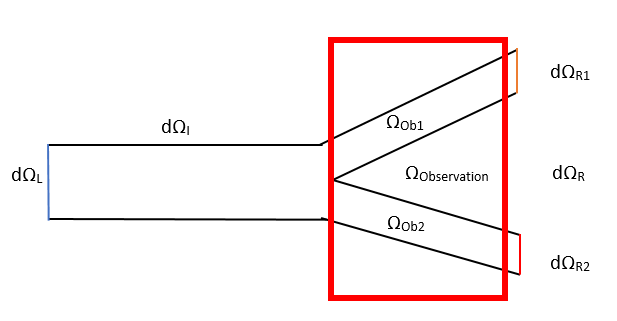
\includegraphics[scale=0.8]{observation.png}
	\caption{Domain of Interest}
	\label{Observation1}
\end{figure}
The first problem of interest is of the form:
\begin{align*}
&\min_{\Sta, w} \quad \frac{1}{2}|| \Sta -\widehat \Sta||^2_{L_2( \Sigma_{Ob})} + \frac{\beta}{2}||w||^2_{L_2(\Sigma)}\\
&\text{subject to:}\\
&\partial_t \rho = \nabla^2 \rho - \nabla \cdot (\rho \mathbf{w}) +\nabla \cdot (\rho \nabla V_{ext}) + \nabla \cdot \int_\Omega \rho(r) \rho(r') \nabla V_2(|r-r'|) dr' + w \quad  \text{in} \quad \Sigma\notag\\
& \rho = \rho_0 \quad \text{at} \quad t=0 \notag\\
& - \mathbf{j} \cdot \nor = \mathbbm{1}_{\partial \Omega_L}( C_{L1}  + C_{L2}\Sta) +\mathbbm{1}_{\partial \Omega_R} ( C_{R1}  + C_{R2}\Sta) +\mathbbm{1}_{\partial \Omega_I} 0 \ \quad \quad\qquad\qquad  \qquad \text{on} \quad \partial \Omega, 
\end{align*}
where $C_{L1}, C_{L2}, C_{R1}$, $C_{R2}$ are constants and $\mathbbm{1}$ is the indicator function of the set of interest. Considering Figure \ref{Observation1}, the stated non-constant flux boundary condition provides the option of describing a non-constant inflow on boundary $\partial \Omega_L$ and a non-constant outflow on $\partial \Omega_R$, while keeping a no flux condition on the rest of the boundary, denoted by $\partial \Omega_I$.
Furthermore, $\mathbf{j}$ satisfies:
\begin{align*}
\mathbf{j}=\nabla \rho - (\rho \mathbf{w}) +(\rho \nabla V_{ext}) +  \int_\Omega \rho(r) \rho(r') \nabla V_2(|r-r'|) dr'.
\end{align*}
Moreover, let $\widehat \Sta$ be defined such that:
\begin{align*}
\widehat \Sta = \mathbbm{1}_{ \Omega_{Ob1}} \tilde \Sta  +\mathbbm{1}_{ \Omega_{Ob2}} 0.
\end{align*}
This describes a desired state where the particle mass accumulates in the observation domain $\Omega_{Ob1}$ and no particles are found in $\Omega_{Ob1}$. Since observations are only taken on $\Omega_{Ob}$, there is no prescribed desired state on $\Omega / \Omega_{Ob}$.\\
The Lagrangian is of the form:
\begin{align*}
\mathcal{L}(\Sta,w,\Adjb,\Adjc ) &=\frac{1}{2} \int_0^T \int_{\Omega_{Ob}} (\Sta - \widehat \Sta)^2 dr dt + \frac{\beta}{2}\int_0^T \int_\Omega w^2 drdt \\
&+ \int_0^T \int_\Omega \bigg( \partial_t \rho - \nabla^2 \rho + \nabla \cdot (\rho \mathbf{w}) -\nabla \cdot (\rho \nabla V_{ext}) \\
&+ \nabla \cdot \int_\Omega \rho(r) \rho(r') \nabla V_2(|r-r'|) -w \bigg) \Adjb dr dt\\
&+ \int_0^T \int_{\partial \Omega} \bigg(  \bigg(-\nabla \rho+ (\rho \mathbf{w}) -(\rho \nabla V_{ext}) -  \int_\Omega \rho(r) \rho(r') \nabla V_2(|r-r'|) dr' \bigg)\cdot \nor\\
&  -\mathbbm{1}_{\partial \Omega_L}( C_{L1}  + C_{L2}\Sta) -\mathbbm{1}_{\partial \Omega_R} ( C_{R1}  + C_{R2}\Sta) -\mathbbm{1}_{\partial \Omega_I} 0 \bigg) \Adjc dr dt.
\end{align*}
The derivative of $\mathcal{L}$ with respect to $\rho$ is, as taken from the extended project, is:
\begin{align*}
&\mathcal{L}_\rho (\rho,{w},\Adjb,\Adjc)h=
\int_\Omega h(T) \Adjb(T) dr\\
&+ \int_0^T \int_\Omega \bigg( \mathbbm{1}_{ \Omega_{Ob}} (\rho- \widehat{\rho})  - \partial_t \Adjb  - \nabla \Adjb \cdot \mathbf{w}  - \nabla^2 \Adjb \notag 
+  \nabla \Adjb \cdot \nabla V_{ext}  \notag \\
&+ \int_\Omega (\nabla  \Adjb(r)+\nabla  \Adjb(r')) \rho(r') \nabla V_2(|r-r'|) dr'+ \int_{\partial \Omega} ( \Adjc(r') - \Adjb(r')) \rho(r')   \frac{\partial V_2(|r-r'|)}{\partial n} dr' \bigg) h dr dt \\
&+  \int_0^T\int_{\partial \Omega}  \bigg(
\bigg(\frac{\partial \Adjb }{\partial n} + \Adjb  \mathbf{w} \cdot \mathbf{n} - \Adjc \mathbf{w} \cdot \mathbf{n}  +  \Adjc \dfrac{\partial V_{ext}}{\partial n} - \Adjb \frac{\partial V_{ext}}{\partial n} + ( \Adjc - \Adjb)  \int_\Omega \rho(r') \frac{\partial V_2(|r-r'|)}{\partial n} dr'\\
& -\mathbbm{1}_{\partial \Omega_L} C_{L2} \Adjc   -\mathbbm{1}_{\partial \Omega_R} C_{R2} \Adjc \bigg)h + \bigg( \Adjc- \Adjb \bigg) \frac{\partial h}{\partial n} \bigg) dr dt =0.
\end{align*}
Then, from appropriate analysis we find that:
\begin{align*}
\Adjc = \Adjb,
\end{align*}
and therefore we get:
\begin{align*}
\mathbbm{1}_{\Omega_{Ob}}(\rho- \widehat{\rho})   - \partial_t  \Adjb  - \nabla \Adjb \cdot \mathbf{w}  - \nabla^2 \Adjb \notag 
+  \nabla \Adjb \cdot \nabla V_{ext}  \notag \\
+ \int_\Omega (\nabla  \Adjb(r)+\nabla  \Adjb(r')) \rho(r') \nabla V_2(|r-r'|) dr' &=0, \quad \text{in} \quad \Sigma, \\
\frac{\partial \Adjb }{\partial n}  -\mathbbm{1}_{\partial \Omega_L} C_{L2} \Adjb   -\mathbbm{1}_{\partial \Omega_R} C_{R2} \Adjb&=0, \quad \text{on} \quad \partial \Omega.
\end{align*}
In particular, this is:
\begin{align*}
\mathbbm{1}_{\Omega_{Ob1}}(\rho- \widehat{\rho}) +\mathbbm{1}_{\Omega_{Ob2}}\rho  - \partial_t  \Adjb  - \nabla \Adjb \cdot \mathbf{w}  - \nabla^2 \Adjb \notag 
+  \nabla \Adjb \cdot \nabla V_{ext}  \notag \\
+ \int_\Omega (\nabla  \Adjb(r)+\nabla  \Adjb(r')) \rho(r') \nabla V_2(|r-r'|) dr' &=0, \quad \text{in} \quad \Sigma, \\
\frac{\partial \Adjb }{\partial n}  -\mathbbm{1}_{\partial \Omega_L} C_{L2} \Adjb   -\mathbbm{1}_{\partial \Omega_R} C_{R2} \Adjb&=0, \quad \text{on} \quad \partial \Omega.
\end{align*}
The gradient equation is:
\begin{align*}
w = \frac{1}{\beta}\Adjb.
\end{align*}
Comparing this to the previous section, it can be observed that the gradient equations have opposite signs. This is due to a different construction of the Lagrangian.



	

The problem of interest is of the form:
\begin{align*}
&\min_{\Sta, \Con} \quad \frac{1}{2}|| \Sta -\hat \Sta||^2_{L_2(\partial Q_R)} + \frac{\beta}{2}|| \Con||^2_{L_2(Q)}\\
\text{subject to:}\\
&\partial_t \rho = \nabla^2 \rho - \nabla \cdot (\rho \mathbf{w}) +\nabla \cdot (\rho \nabla V_{ext}) + \nabla \cdot \int_\Omega \rho(r) \rho(r') \nabla V_2(|r-r'|) dr' + \Con \quad  \quad\text{in} \quad Q,\notag\\
& \rho = \rho_0 \quad \text{at} \quad t=0 \notag\\
& - \mathbf{j} \cdot \nor = \mathbbm{1}_{\partial \Omega_L}( C_{L1}  + C_{L2}\Sta) +\mathbbm{1}_{\partial \Omega_R} ( C_{R1}  + C_{R2}\Sta) +\mathbbm{1}_{\partial \Omega_I} 0, \quad  \quad\text{on} \quad \partial Q, 
\end{align*}
where $C_{L1}, C_{L2}, C_{R1}$, $C_{R2}$ are constants and $\mathbbm{1}$ is the indicator function of the set (the parts of the boundary) of interest.
Furthermore, $\mathbf{j}$ satisfies:
\begin{align*}
\mathbf{j}=\nabla \rho - (\rho \mathbf{w}) +(\rho \nabla V_{ext}) +  \int_\Omega \rho(r) \rho(r') \nabla V_2(|r-r'|) dr'.
\end{align*}
Moreover, let $\hat \Sta$ be defined such that:
\begin{align*}
\hat \Sta = \mathbbm{1}_{\partial \Omega_{R1}} \tilde \Sta  +\mathbbm{1}_{\partial \Omega_{R2}} 0.
\end{align*}

\subsection*{The Lagrangian}
The Lagrangian is of the form:
\begin{align*}
\mathcal{L}(\Sta,\Con,\Adja,\Adjc ) &= \int_0^T \int_{\partial \Omega_R} \frac{1}{2}(\Sta - \hat \Sta)^2 dr dt + \frac{\beta}{2}\int_0^T \int_\Omega \Con^2 drdt \\
&+ \int_0^T \int_\Omega \bigg( \partial_t \rho - \nabla^2 \rho + \nabla \cdot (\rho \mathbf{w}) -\nabla \cdot (\rho \nabla V_{ext}) + \nabla \cdot \int_\Omega \rho(r) \rho(r') \nabla V_2(|r-r'|) \bigg) \Adja dr dt\\
&+ \int_0^T \int_{\partial \Omega} \bigg(  \bigg(-\nabla \rho+ (\rho \mathbf{w}) -(\rho \nabla V_{ext}) -  \int_\Omega \rho(r) \rho(r') \nabla V_2(|r-r'|) dr' \bigg)\cdot \nor\\
&  -\mathbbm{1}_{\partial \Omega_L}( C_{L1}  + C_{L2}\Sta) -\mathbbm{1}_{\partial \Omega_R} ( C_{R1}  + C_{R2}\Sta) -\mathbbm{1}_{\partial \Omega_I} 0 \bigg) \Adjc dr dt.
\end{align*}

\subsection*{The Adjoint Equation}
The derivative of $\mathcal{L}$ with respect to $\rho$ is, as taken from the extended project:
\begin{align*}
&\mathcal{L}_\rho (\rho,\mathbf{w},p_\Omega,p_{\partial \Omega})h=
\int_\Omega h(T) \Adja(T) dr\\
&+ \int_0^T \int_\Omega \bigg(   - \partial_t \Adja  - \nabla \Adja \cdot \mathbf{w}  - \nabla^2 \Adja \notag 
+  \nabla \Adja \cdot \nabla V_{ext}  \notag \\
&+ \int_\Omega (\nabla  \Adja(r)+\nabla  \Adja(r')) \rho(r') \nabla V_2(|r-r'|) dr'+ \int_{\partial \Omega} ( \Adjc(r') - \Adja(r')) \rho(r')   \frac{\partial V_2(|r-r'|)}{\partial n} dr' \bigg) h dr dt \\
&+  \int_0^T\int_{\partial \Omega}  \bigg(
\bigg(\frac{\partial \Adja }{\partial n} + \Adja  \mathbf{w} \cdot \mathbf{n} - \Adjc \mathbf{w} \cdot \mathbf{n}  +  \Adjc \dfrac{\partial V_{ext}}{\partial n} - \Adja \frac{\partial V_{ext}}{\partial n} + ( \Adjc - \Adja)  \int_\Omega \rho(r') \frac{\partial V_2(|r-r'|)}{\partial n} dr'\\
&\mathbbm{1}_{\partial \Omega_R} (\rho- \hat{\rho}) -\mathbbm{1}_{\partial \Omega_L} C_{L2} \Adjc   -\mathbbm{1}_{\partial \Omega_R} C_{R2} \Adjc \bigg)h + \bigg( \Adjc- \Adja \bigg) \frac{\partial h}{\partial n} \bigg) dr dt =0.
\end{align*}
Then, from appropriate analysis we find that:
\begin{align*}
\Adjc = \Adja,
\end{align*}
and therefore we get:
\begin{align*}
- \partial_t  \Adja  - \nabla \Adja \cdot \mathbf{w}  - \nabla^2 \Adja \notag 
+  \nabla \Adja \cdot \nabla V_{ext}  \notag \\
+ \int_\Omega (\nabla  \Adja(r)+\nabla  \Adja(r')) \rho(r') \nabla V_2(|r-r'|) dr' &=0, \quad \text{in} \quad Q, \\
\frac{\partial \Adja }{\partial n}+ \mathbbm{1}_{\partial \Omega_R} (\rho- \hat{\rho}) -\mathbbm{1}_{\partial \Omega_L} C_{L2} \Adja   -\mathbbm{1}_{\partial \Omega_R} C_{R2} \Adja&=0, \quad \text{on} \quad \partial Q.
\end{align*}
Again, in particular the boundary condition is:
\begin{align*}
\frac{\partial \Adja }{\partial n}+ \mathbbm{1}_{\partial \Omega_{R1}}(\rho- \tilde{\rho} -C_{R2} \Adja) + \mathbbm{1}_{\partial \Omega_{R2}} (\Sta-C_{R2} \Adja) - \mathbbm{1}_{\partial \Omega_L} C_{L2} \Adja   &=0, \quad \text{on} \quad \partial Q.
\end{align*}

	
	
	
	
	
	
	\section{Numerical Methods for PDECO}
	
	\subsection{Standard Approaches}
		\begin{itemize}
			\item Newton -Krlov, GMRES explanation, ...
			\item Fixed Point
			\item Preconditioning
		\end{itemize}
	
	\subsection{Optimization Methods we use}
	Difference to above: above general review, here what we have been doing.
		\begin{itemize}
			\item Fixed Point (+ Armijo Extension)
			\item Newton-Krylov
			\item Picard Multiple Shooting
			\item fsolve Multiple Shooting 
			\item fsolve algorithms in Matlab
		\end{itemize}
	
	\subsubsection{Newton-Krylov Algorithm}
	\subsubsection{Fixed Point Algorithm}\label{sec:Method_SolverFP}	
	In this section we describe the fixed point algorithm, which is an efficient and stable optimization method for the optimal control problems considered above. 
We denote the discretized versions of the variables $\rho$, $\adj$ and $\mathbf{w}$ with $P$, $Q$ and $W$, respectively. Each of these matrices is of the form $A = [\boldsymbol{a_0}, \boldsymbol{a_1}, ... ,\boldsymbol{a_n}]$, where the vectors $\boldsymbol{a_k}$ represent the solutions at the discretized times $k \in 0,1,....,n$, where $n$ is the number of time points. In particular, the first column of $P$, denoted by $\boldsymbol{\rho_0}$, corresponds to the initial condition $\rho(r,0)$. If the spatial domain is one-dimensional, $P$, $Q$ and $W$ are of size $N \times (n + 1)$, where $N$ is the number of spatial points. In the two-dimensional case, $P$ and $Q$ are of size $(N_1N_2) \times (n + 1)$, where $N_1$ is the number of spatial points in the direction of $x_1$ and $N_2$ the points along the $x_2$ axis. Generally, $N_1 = N_2$. The discretized control $W$ for linear control problems is also $(N_1N_2) \times (n + 1)$ dimensional, while it is $(2N_1N_2) \times (n + 1)$ dimensional for nonlinear control problems. This is due to the fact that the control is represented by a vector field, when applied nonlinearly.
\\
\\
The optimization algorithm is initialized with a guess for the control, $W^{(0)}$. Then, in each iteration, denoted by $i$, the following steps are computed:
\vspace{0.1cm}
\begin{enumerate}
	\item Starting with a guess for the control $W^{(i)}$ as input variable, the corresponding state $P^{(i)}$ is found by solving the forward equation.
	\item In a next step, the value of the adjoint, $Q^{(i)}$, is established by computing the adjoint equation, using $W^{(i)}$ and $P^{(i)}$ as inputs. Since $P^{(i)}$ contains the solution for all discretized times $k \in 0,1,...,n$, this circumvents issues resulting from the non-local coupling in time, resulting from reversing time in the adjoint equation. As illustrated in the same section, time is reversed in the adjoint equation, so that the result is a matrix $\tilde{Q}^{(i)} =  [\boldsymbol{\adj_n},\boldsymbol{\adj_{n-1}}, ..., \boldsymbol{\adj_1} ]$. The columns of $\tilde{Q}^{(i)}$ are permuted to obtain the solution  $Q^{(i)}$.
	\item The gradient equation is solved, given the solutions $P^{(i)}$ and $Q^{(i)}$. This results in a new value for the control, $W^{(i)}_g$.
	\item  The convergence of the optimization scheme is measured by computing the error between $W^{(i)}$ and $W^{(i)}_{g}$. The error measure, $\mathcal{E}$, is discussed in detail in Section \ref{sec:ErrorMeasure}. 
	\begin{itemize}
		\item  If this error is lower than a set tolerance, the optimality system is self-consistent. This implies that the solution triplet ($\bar{P},\bar{W},\bar{Q}$) solves the (discretized) optimality system, and is therefore an optimal solution to the PDE-constrained optimization problem of interest.
		\item If the error is above the optimality tolerance, Step 5 is executed.
	\end{itemize}
	\item Finally, the update $W^{(i+1)}$ is a linear combination of the current guess $W^{(i)}$, and the value obtained in Step 3, $W^{(i)}_{g}$, employing a mixing rate $\lambda \in [0,1]$:
	\begin{align*}
	W^{(i+1)} = (1-\lambda)W^{(i)} + \lambda W^{(i)}_{g}.
	\end{align*}
	The guess for the control is updated from $W^{(i)} $ to $W^{(i+1)} $ and Steps 1-5 are repeated until the method converges. 
\end{enumerate}
\vspace{0.3cm}
The update scheme in Step 5, with mixing rate $\lambda$, is known to stabilise fixed point methods, see \cite{Roth1}. Typical values of $\lambda$, which provide stable convergence, lie between $0.1$ and $0.001$. Throughout this paper, $\lambda =0.01$, unless stated otherwise. This mixing scheme is similar to the updating scheme presented in~\cite{Burger1}. 
Note that, while the solutions $P^{(i)}$ and $Q^{(i)}$ change in each iteration, the initial condition $\boldsymbol{\rho_0}$ and final time condition $\boldsymbol{\adj_n}$ remain unchanged throughout the process. Therefore, the only variable inducing a change in the solution is $W^{(i)}$.
	\subsubsection{Picard Multiple Shooting}
	
The multiple shooting algorithm, introduced in the first year report, has been extended by employing a Picard mixing scheme to replace the {\scshape MATLAB} inbuilt solver \texttt{fsolve}. In the following, this is briefly outlined.
The idea of the updating scheme is similar to the one presented for the fixed point algorithm. However, while the fixed point algorithm updates through the control variable, the fixed point algorithm updates via the variables $\rho$ and $q$.
The multiple shooting method consists of discretizing the time interval and solving the optimality system on each interval individually. This is done because of the non-local time coupling of the forward and adjoint equations. It requires the input of an initial guess at each discretized time point for each of the variables. The aim of the optimization solver is then to minimize the distance between the initial guesses and numerical solutions of the variables at each of the time points. \\
The Picard mixing scheme is a fixed point type algorithm. At each iteration $i$ it takes a set of guesses at the discretized time points, denoted by $Y_i$. The matrix $Y = [P,Q]$ contains the discretized values for the variables $\rho$ and $q$, denoted by $P$ and $Q$, analogously to the previous section.  
The system of PDEs is solved on each of the discretized intervals and a new set of variable values at the time points is created, denoted by $Y_{out}$. Then, the mixing scheme provides a new guess for the iteration $i+1$:
\begin{align*}
Y_{i+1} = (1 - \lambda)Y_i + \lambda Y_{out},
\end{align*}
where $\lambda$ is the mixing rate. It typically takes values between $0.1$ and $0.01$, depending on the complexity of the system to solve. Choosing a relatively small value of $\lambda$ stabilizes the algorithm. 
The algorithm terminates when the system of PDEs is solved self-consistently, i.e. when the distance between $Y_i$ and $Y_{out}$ is small, as measured in a chosen norm. The most frequently applied norm is discussed in Section \ref{sec:ErrorMeasure}.
This algorithm is working very well for examples involving the overdamped equations. However, the fixed point algorithm provides an even simpler method, which does not require the solution of the optimality system on small time intervals and is therefore even quicker. Since we will apply the numerical optimization method to increasingly difficult optimal control problems in the future, the multiple shooting algorithm may provide more numerical stability for numerically harder problems and is therefore a relevant tool to consider in the future. Changing the optimization solver in the implementation is straightforward and only requires changing a flag in the input file.
\\
A challenge with this solver is, that it needs to be provided with good initial guesses for the variables $\rho$ and $\adj$ at the discretized time points. The guess for $\rho$ can be obtained by solving the associated forward problem and using the result as a first guess. However, a good guess for $\adj$ is trickier to obtain. One way of doing so is by using the gradient equation, which relates $\rho$, $\adj$ and $\mathbf w$, the control. Since the input for the forward control is known, one can use this information, together with the initial guess for $\rho$, to construct an initial guess for $\adj$. 
One challenge however arises when considering the flow control problem involving the overdamped equations. The gradient equation is $\mathbf{w} = - \frac{1}{\beta} \rho\nabla \adj$. In order to derive the value of $\adj$ from this equation, we need to divide by $\rho$, making use of the assumption that $\rho$ is strictly positive, and integrate over the whole space. The issue here is that integration introduces an indeterminable constant. Furthermore, if Dirichlet boundary conditions are applied, the strict positivity of $\rho$ is in question.\\
An alternative method of obtaining an initial guess for $\adj$ is to perform one step of the fixed point method.

	\subsubsection{Multiple Shooting}
	Boundary value problem (BVP) solvers, such as \texttt{bvp4c}, are designed to treat BVPs in time, see \cite{bvp4cPaper1}. Therefore, they are not equipped to deal with BVPs in both space and time. A method has to be developed that circumvents using BVP solvers and uses initial value problem (IVP) solvers instead. This strategy is called multiple shooting and the theoretical derivation of a multiple shooting approach for PDE-constrained optimization problems can be found in \cite{CarraroIndMultipleShooting} and \cite{CarraroDirectIndirectMultipleShooting}.
\\
In this section, the numerical method is described at the different stages of its development. 
The PDE constraint considered has either Dirichlet or Neumann boundary conditions in space. The problem is treated in one and two dimensions. In order to initiate the development of the method, a simpler PDE constrained optimization problem is considered at first. Once the method is established for the simpler problem, the non-local term is added. After that, two dimensional problems are considered.

\subsubsection*{One-Dimensional Diffusion} \label{secNumericsOneDDiffusion1}
One of the simplest cases of a PDE-constrained optimization problem is heat control in one dimension. The PDE constraint involved is the forced heat equation, and the PDE-constrained optimisation problem (\ref{sysOptimalHeating1}), derived in Section \ref{secExactSolsDiffusion1}, is used, and the derived optimality system is treated below. 

The first step in solving this optimality system is to substitute the gradient equation into the heat equation for $u$ and rearranging the equations to only have the time derivative on the left-hand side.
This results in a coupled system of PDEs: 
\begin{align}\label{sysOneDimHeatEqunOptisys1}
\partial_t \rho(r,t) &= \partial_{rr}\rho(r,t) + \frac{1}{\beta}p(r,t),\\
\partial_t p(r,t) &= - \partial_{rr} p(r,t) + \rho(r,t) -\hat{\rho}(r,t), \notag \\
\text{Initial } & \text{and  Final-Time Conditions:}\notag\\
\rho(r,0)&=\rho_0(r),\notag\\
p(r,T) &=0,\notag\\
\text{Dirich} &\text{let  Boundary Conditions:}\notag\\
\rho(r,t) &=0,\quad \text{on} \quad \partial \Omega,\notag\\
p(r,t) &=0,\quad \text{on} \quad \partial \Omega,\notag
\end{align}
where $r \in [a,b]$ and $t \in [0,T]$.
This system is considered as a test problem, since exact solutions for $\rho$ and $p$ are known. Therefore, the exact error of the numerical method can be determined at all points in space and time. The derivation of the exact solutions are discussed in Section \ref{secExactSolsDiffusion1}.

The method that is used to solve this system of PDEs is called the shooting method.
The procedure is to first discretize the problem in space, that is to replace the space derivatives with the appropriate Chebyshev differentiation matrices, as defined above. Then the problem reduces to a coupled system of ODEs, which can be solved using an ODE solver, such as the Matlab solver \texttt{ode15s}. The challenge is that the optimality system is a boundary value problem in time, since the adjoint equation has a final time condition in $p$. 
Therefore, the first idea is to create a guess for the initial condition $p_0(r)$, solve the coupled ODE system using this guess, extracting the computed $p$ value at the final time, $p_{co}(T)$ and measuring the error between the computed $p_{co}$ and the exact $p_{ex}$:
\begin{align*}
e= \norm{p_{co}(T) - p_{ex}(T)}.
\end{align*}
The final step in this procedure is to minimize this error by varying $p_0(r)$, using an in-built Matlab optimization routine, such as \texttt{fsolve}.
This is easily implemented in Matlab, see Appendix \ref{ShootingTest1DiffusionLineBlowsUp}.
However, the problem with this approach is that the adjoint equation, written in this form, is not well posed. The solution to this system blows up in finite time, which is caused by the negative diffusion term in the PDE for $p$.\\

Therefore, the adjoint equation has to be rewritten. This is done by rescaling time as
\begin{align*}
\tau=T+t_0-t,
\end{align*}
which causes the adjoint equation to run backwards in time from $T$ to $t_0=0$. This changes the final time condition for $p$ at time $t=T$, $p(T)=0$, into an initial condition at time $\tau =0$, ${p}(0)=0$.
The optimality system is then:
\begin{align} \label{sysOptimDiffAdjBW1}
\partial_t \rho(r,t) &= \partial_{rr} \rho(r,t) + \frac{1}{\beta}{p}(r,t), \\
\partial_t {p}(r,\tau) &=\partial_{rr} {p}(r,\tau) - \rho(r,\tau) +\hat{\rho}(r,\tau), \notag \\
\text{Initial   } & \text{ Conditions:} \notag  \\
 \rho(r,0)&=\rho_0(r),  \quad \text{for} \quad t=0,\notag \\
{p}(r,0) &=0, \quad \text{for} \quad \tau=0,\notag \\
\text{Dirich} &\text{let Boundary Conditions:} \notag \\
\rho(a,t) &=\rho(b,t)=0, \notag \\
{p}(a,\tau) &={p}(b,\tau)=0, \notag 
\end{align} 
where $t \in [t_0,T]$ and $\tau \in [T,t_0]$.
This is now well posed. However, the issue with this rewritten system is that information about $\rho$ at later times is needed to solve the adjoint equation and ${p}$ values for earlier times are needed to solve the state equation, while neither of these information is available. Figure \ref{ShootingMethod1} visualises this problem. The initial conditions for $\rho$ and $p$ are represented as a green and blue dot respectively. Time $t$ is represented by the green arrow, while time $\tau$, the backwards time, is represented by a blue arrow. In order to test whether this approach works, the exact solution for $\rho$ and $q$ can be used, where information is missing. Then the problem is a decoupled system of PDEs, which is straightforward to solve.  


%\begin{figure}[h] 
%		\vspace{-20pt}
%	\centering
%	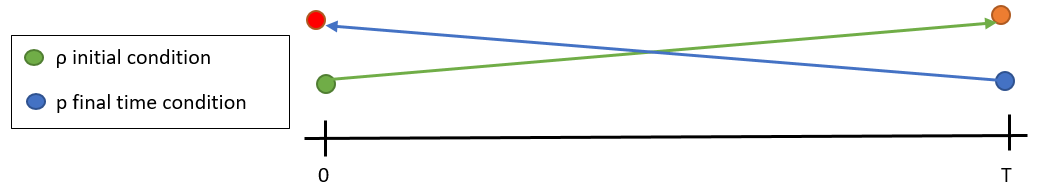
\includegraphics[scale=0.85]{FullSol.png}
%		\vspace{-10pt}
%    \caption{Solving a coupled system of PDEs on $[0,T]$.} 
%    \label{ShootingMethod1}
%    	\vspace{-10pt}
%\end{figure}


In order to replace the missing information, as illustrated above, interpolation is used. Since interpolation using only the endpoints of the interval $[t_0,T]$ would be highly inaccurate, a strategy, called multiple shooting, is exploited in this section. 
The time interval is divided into a number of $n$ subintervals, such that $t_0 < t_1<t_2<...<t_n=T$. The subintervals are denoted by $I_i$, where $i=0,1,...,n-1$. The values for $\rho$ and ${p}$ at these times constitute the initial guess. The discretization of the time interval and initial guesses for $\rho$ and $p$ are illustrated in Figure \ref{ShootingMethod2}. The initial guess can be obtained by different methods, which will be discussed in a later section.

%\begin{figure}[h] 
%	\centering
%	\vspace{-10pt}
%	\includegraphics[scale=0.9]{FullDiscr.png}
%		\vspace{-10pt}
%	\caption{Discretizing the time interval and obtain initial guesses for $\rho$ and $q$.} 
%	\label{ShootingMethod2}
%	\vspace{-10pt}
%\end{figure}

In a first step, these initial guesses are chosen to be the known exact solutions to $\rho$ and ${p}$ at the specified times $t_i$. 
The optimality system (\ref{sysOptimDiffAdjBW1}) is solved on each of the $I_i$, by considering the upper and lower bound of the subinterval, $t_i$ and $t_{i+1}$ instead of the global bounds $t_0$ and $T$. The new backward running time is defined, equivalently to above, as $\tilde\tau =t_{i+1}+t_i-t$, and the system becomes:
\begin{align} \label{sysOptimDiffAdjBW2}
\partial_t \rho(r,t) &= \partial_{rr}\rho(r,t) + \frac{1}{\beta}{p}(r,t), \\
\partial_t {p}(r,\tilde\tau) &= \partial_{rr}{p}(r,\tilde\tau) - \rho(r,\tilde\tau) +\hat{\rho}(r,\tilde\tau), \notag \\
\text{Initial   } & \text{ Conditions:} \notag  \\
\rho(r,t_i)&=\rho_{t_i}, \quad \ \ \text{for} \ \quad t=t_i, \notag \\
{p}(r,t_{i+1}) &=p_{t_{i+1}}, \quad \text{for} \quad \tilde t=t_{i+1}, \notag \\
\text{Dirich} &\text{let  Boundary Conditions:} \notag \\
\rho(a,t) &=\rho(b,t)=0, \notag \\
{p}(a,\tilde\tau) &={p}(b,\tilde\tau)=0, \notag 
\end{align} 
where $t \in I_{i}=[t_i,t_{i+1}]$.
On each subinterval, both $\rho$ and ${p}$ are interpolated between their known values at $t_i$ and $t_{i+1}$, and the result is used to provide $\rho$ at a later time step, to solve the adjoint equation, as well as ${p}$ at an earlier time step, to solve the state equation. 
\newline
\newline
In order to implement the strategy, (\ref{sysOptimDiffAdjBW2}) is evaluated on each time interval $I_i=[t_i,t_{i+1}]$, using interpolation for $\rho$ in the adjoint equation and for $ {p}$ in the state equation to provide the missing information.

%\begin{figure}[h] 
%	\centering
%	\vspace{-10pt}
%	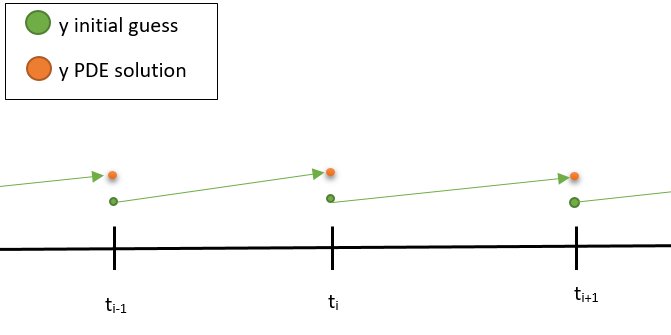
\includegraphics[scale=0.9]{rhoSol.png}
%	\caption{Solution strategy for $\rho$.} 
%	\label{ShootingMethod3}
%\end{figure}
%
%\begin{figure}[h] 
%	\centering
%	\vspace{-20pt}
%	\includegraphics[scale=0.9]{pSol.png}
%	\caption{Solution strategy for $p$.} 
%	\label{ShootingMethod4}
%	\vspace{-10pt}
%\end{figure}

As can be observed in Figure \ref{ShootingMethod3}, the value of $\rho$, taken from the ODE solver, at $t_{i+1}$ is compared to $\rho$ at $t_{i+1}$, which is the initial guess for solving (\ref{sysOptimDiffAdjBW2}) on the next interval $I_{i+1}=[t_{i+1},t_{i+2}]$:
\begin{align}\label{eqnErrorINitoptiguess}
e= \norm{g_{init}-g_{sol}},
\end{align} 
where $g_{init}=(g_1,g_2,...g_n)$ is a vector of initial guesses for $\rho$ on all $n$ time points and $g_{sol}$ is the vector of PDE solutions associated with the initial guesses on all time points.
This provides an error measure of the quality of the set of initial guesses $g_{init}$ for $\rho$. This error calculation is repeated for ${p}$, as illustrated in Figure \ref{ShootingMethod4}. However, since ${p}$ is running backwards in time, the solution to the ODE solver provides the value for ${p}$ at $t_i$, the lower bound on the considered interval $I_i$, which is then compared with the initial guess for ${p}$ for the previous interval $I_{i-1}=[t_{i-1},t_i]$.
Note that for this solution strategy any ODE solver can be used to solve the discretized PDE on each subinterval. Furthermore, while pseudospectral methods are the best method for PDE-constrained optimization problems involving integro-PDE constraints, as discussed in Section \ref{secCompareFEMFDMPDM}, it is in principle possible to use other time or space discretization methods.
\subsubsection*{One-Dimensional Diffusion with a Non-Local Term}\label{secOneDDiffusionNonlocalOptim1}
The problem (\ref{sysOptimalHeating1}) is extended by adding a non-local term to the forced heat equation. This non-local term is the two body interaction term that is introduced in Section \ref{secOptimalitySysNonLocal1}.
The one dimensional PDE-constrained optimization problem is:
\begin{align}
&\min_{\rho,u} \quad \frac{1}{2}\norm{\rho- \hat{\rho}}_{L_2}^2 + \frac{\beta}{2} \norm{u}_{L_2}^2,\\
&\text{subject to:}\notag 
\notag \\
&\partial_t \rho - \Delta \rho - u - \nabla \cdot \rho(r) \int_\Omega \nabla V_2(|r-r'|) \rho(r')dr'=0,  \quad \text{in} \quad \Omega,\notag 
\notag \\
&\rho(r,0)=\rho_0(r),\notag 
\notag \\
& \rho(r,t)=0, \quad \text{on} \quad \partial \Omega. \notag 
\end{align}
The first-order optimality system, including the non-local term, is:
\begin{align}\label{sysoptinonlocandheat1D}
\textbf{Adjoint Equation}  \\
\partial_t  p  + \partial_{rr} p + \int_\Omega \bigg(\partial_r  p(r)+\partial_{r'}  p(r')\bigg) \rho(r') \partial_r V_2(|r-r'|) dr' &=(\rho- \hat{\rho})  \quad \text{in} \quad \Omega, \notag \\
p(T) &= 0 \notag\\
p(r,t) &=0 \quad \quad \quad \quad \text{on}\quad \partial\Omega, \notag\\
\textbf{Gradient Equation} \notag \\
\beta u  - \rho  &=0 \quad\quad\quad\quad \text{in} \quad \Omega, \notag \\
\textbf{Forward Problem} \notag \\
\partial_t \rho - \partial_{rr} \rho-u - \partial_r  \rho(r) \int_\Omega \partial_r V_2(|r-r'|) \rho(r')dr' &=0 \quad\quad\quad\quad \text{in} \quad \Omega, \notag \\ 
\rho(r,0)&=\rho_0(r), \notag \\
\rho(r,t) &=0 \quad\quad\quad \quad \text{on} \quad \partial \Omega. \notag
\end{align}
This is directly derived from taking the relevant terms in (\ref{sysFirstOderOptimalityNonLocal1}).
The system that has to be solved on each interval $[t_i,t_{i+1}]$ is, equivalent to (\ref{sysOptimDiffAdjBW2}):
\begin{align*}
\partial_t \rho(r,t) &= \partial_{rr}\rho(r,t) + \frac{1}{\beta}{p}(r,t) + \partial_r  \rho(r,t) \int_\Omega \partial_r V_2(|r-r'|) \rho(r',t)dr', \\
\partial_t {p}(r,\tilde\tau) &= \partial_{rr}{p}(r,\tilde\tau) - \rho(r,\tilde\tau) +\hat{\rho}(r,\tilde\tau) -\int_\Omega \bigg(\partial_r  p(r,\tilde\tau)+\partial_{r'}  p(r',\tilde\tau)\bigg) \rho(r',\tilde\tau) \partial_r V_2(|r-r'|) dr', \notag \\
\text{Initial } & \text{Conditions:} \notag  \\
\rho(r,t_i)&=\rho_{t_i}(r), \quad \quad\text{for} \ \quad t=t_i, \notag \\
{p}(r,t_{i+1}) &=p_{t_{i+1}}(r), \  \quad \text{for} \quad t=t_{i+1}, \notag \\
\text{Dirichl}&\text{et Boundary Conditions:} \notag \\
\rho(a,t) &=\rho(b,t)=0, \notag \\
{p}(a,\tilde\tau) &={p}(b,\tilde\tau)=0, \notag 
\end{align*} 
where $\tilde\tau=t_{i+1} +t_i -t$, as before.
As discussed above, $V_2$ is the force between two particles at positions $r$ and $r'$. It is defined depending on the physical problem involved. For a first numerical test problem, the choice of $V_2$ is a Gaussian:
\begin{align}\label{eqn1Dgaussian}
V_2(x)= \alpha e^{-x^2}.
\end{align}
Then $\partial_r V_2$ satisfies:
\begin{align*}
\partial_r V_2(|r-r'|)= -2\alpha|r-r'| e^{-|r-r'|^2}.
\end{align*}
The specific problem that is solved numerically is:
\begin{align}\label{OptmSysNonloc1alpha}
\partial_t \rho(r,t) &= \partial_{rr}\rho(r,t) + \frac{1}{\beta}{p}(r,t) + \alpha \partial_r  \rho(r,t) \int_\Omega \partial_r  e^{-|r-r'|^2} \rho(r',t)dr', \\
\partial_t {p}(r,\tilde\tau) &= \partial_{rr}{p}(r,\tilde\tau) - \rho(r,\tilde\tau) +\hat{\rho}(r,\tilde\tau) - \alpha\int_\Omega \bigg(\partial_r  p(r,\tilde\tau)+\partial_{r'}  p(r',\tilde\tau)\bigg) \rho(r',\tilde\tau) \partial_r  e^{-|r-r'|^2} dr', \notag \\
\text{Initial } & \text{Conditions:} \notag  \\
\rho(r,0)&=\rho_0(r), \quad \text{for}  \quad t=0, \notag \\
{p}(r,0) &=0,\quad \ \ \quad \text{for} \quad \tilde \tau=0, \notag \\
\notag \\
\text{Dirichl}&\text{et Boundary Conditions:} \notag \\
\rho(a,t) &=\rho(b,t)=0, \notag \\
{p}(a,\tilde\tau) &={p}(b,\tilde\tau)=0. \notag 
\end{align} 

 While the solution method is similar to the approach in Section \ref{secNumericsOneDDiffusion1}, there are two key differences. Firstly, quadrature has to be used, employing (\ref{eqnClenCurtQuad}), to evaluate the integral terms in the optimality system. The other difficulty is that no exact solutions exist to this problem because of the complexity of the non-local term. Therefore, the main issue in solving (\ref{OptmSysNonloc1alpha}) is finding an initial guess on the Chebyshev time points $t_i$, which is close enough to the solution of the system, so that convergence to a continuous solution on the whole interval is possible. The initial guess is found by using a technique called continuation.
 \\
The parameter $\alpha$ in (\ref{OptmSysNonloc1alpha}) represents the strength of the contribution of the integral term to the system of PDEs. 
It can be varied to choose the strength of the particle interactions on the PDE solution. If $\alpha_0=0$, there is no particle interaction and the optimality system for the forced heat equation is recovered, compare to (\ref{sysOptimDiffAdjBW2}).
 Since the solution to that problem is known, the idea is to use the exact solution to the problem where $\alpha_0=0$ as an initial guess to the problem where $\alpha_1$ is non-zero but small.
The optimal initial guess for the problem involving $\alpha_1$ is found by multiple shooting and used as an initial guess for the problem with $\alpha_2$, where $\alpha_2>\alpha_1$. This process is repeated iteratively until a certain contribution of the integral term is reached, for example $\alpha=1$. 
\newline
Generally, the step size in $\alpha$ is not determined linearly, but chosen adaptively. This is because some parts of the problems may be easier to solve than others. If the change in $\alpha$ is chosen small, then the optimization function only needs a few iteration to find the optimal initial guess, based on the result of the previous step in $\alpha$. This is because the problem with $\alpha_{i+1}$ is similar to the problem involving $\alpha_i$ and therefore the optimal initial guesses for the two problems are close. The downside of this approach is that the problem has to be re-evaluated for many different values of $\alpha$, which is computationally expensive. If $\alpha_{i+1}$ is chosen to be considerably larger than $\alpha_i$ at each step, the problem has to be solved less times. However, the risk is that the optimal initial guess for the problem with $\alpha_i$ is not a suitable initial guess for the problem with $\alpha_{i+1}$, and that no solution is found.
There are many ways to change $\alpha$ adaptively and it depends greatly on the problem that is to be solved. 

\subsubsection*{Two-Dimensional Problems}\label{sec2Dprobsnum1}
The two dimensional version of the PDE constrained optimization problem (\ref{sysOptimalHeating1}) is treated with numerical methods equivalent to the ones used in one-dimensional case, as discussed in Section \ref{secNumericsOneDDiffusion1}. 
The corresponding optimality system is (\ref{sysPotimaltiyheatequn1}).
All the solution methods follow directly from the one-dimensional method presented in Section \ref{secNumericsOneDDiffusion1}. The only difference is that, instead of having a one-dimensional set of spatial Chebyshev points, a two-dimensional Chebyshev grid has to be used, making use of Kronecker products. This has been introduced in Section \ref{secPSMTheory1}.
One of the things to note is that the computational effort in two dimensions is much higher than for one dimensional calculations. This is because instead of $N$ spatial points, $N_1 \times N_2$ spatial points have to be evaluated.

\subsubsection*{Two-Dimensional Problems with a Non-Local Term}
Adding a non-local term to (\ref{sysOptimalHeating1}), the PDE-constrained optimization problem becomes:
\begin{align*}
&\min_{\rho,u} \quad \frac{1}{2}\norm{\rho- \hat{\rho}}_{L_2}^2 + \frac{\beta}{2} \norm{u}_{L_2}^2,\\
\\
&\text{subject to:}\\
&\partial_t \rho = \Delta \rho + {u} + \nabla \cdot \int_\Omega \rho(r) \rho(r') \nabla V_2(|r-r'|)dr'  \quad \text{in} \quad \Omega,
\\
&\rho(r,0)=\rho_0(r),
\\
& \rho(r,t)=0, \quad\quad\quad\quad\quad\quad\quad\quad\quad\quad\quad\quad\quad\quad\quad\quad \quad  \text{on} \quad \partial \Omega,
\end{align*}
where $r=(x,y) \in \mathbf{R}^2$.
The corresponding optimality system is:
\begin{align*}
\textbf{Adjoint Equation}  \\
\partial_t p(r,\tau) &= \Delta p(r,\tau) -\rho(r,\tau) +\hat{\rho}(r,\tau)\\
&-\int_\Omega \bigg( \nabla_r p(r,\tau) + \nabla_{r'} p(r',\tau) \bigg) \rho(r',t) \nabla_r V_2(|r-r'|)dr'  \quad\quad\quad   \text{in} \quad \Omega,\\
p(T) &= 0 \notag\\
p(r,t) &=0 \quad \quad \quad  \quad\quad\quad\quad\quad\quad\quad\quad\quad\quad\quad\quad\quad\quad\quad\quad\quad\quad\quad\quad \quad\ \ \ \text{on}\quad \partial\Omega, \notag\\
\textbf{Gradient Equation} \notag \\
\beta u  - \rho  &=0 \quad\quad\quad\quad \quad\quad\quad\quad\quad\quad\quad\quad\quad\quad\quad\quad\quad\quad\quad\quad\quad\quad\quad\quad\quad\text{in} \quad \Omega, \notag \\
\textbf{Forward Problem} \notag \\
\partial_t \rho(r,t) &= \Delta \rho(r,t) + u(r,t)+  \nabla_r \cdot \int_\Omega \rho(r,t) \rho(r',t) \nabla_r V_2(|r-r'|)dr' \quad \ \text{in} \quad \Omega,\\  
\rho(r,0)&=\rho_0(r), \notag \\
\rho(r,t) &=0 \quad\quad\quad \quad\quad\quad\quad\quad\quad\quad\quad\quad\quad\quad\quad\quad\quad \quad\quad\quad\quad\quad\quad\quad \ \ \ \text{on} \quad \partial \Omega, \notag
\end{align*}
compare with the one-dimensional system (\ref{sysoptinonlocandheat1D}).
Equivalently to the one-dimensional particle interaction term, (\ref{eqn1Dgaussian}), $V_2$ is the two-dimensional Gaussian:
\begin{align*}
V_2(x,y)= \alpha e^{-(x^2 +y^2)}.
\end{align*}
When substituting the gradient equation into the state equation, the optimality system becomes:
\begin{align}\label{OptmSysNonloc1alpha2D}
\partial_t \rho(r,t) &= \Delta\rho(r,t) + \frac{1}{\beta}{p}(r,t) + \alpha \nabla_r \cdot  \int_\Omega \nabla_r\bigg(  e^{-|r-r'|^2} \bigg)\rho(r',t)\rho(r,t)dr', \\
\partial_t {p}(r,\tilde\tau) &=\Delta {p}(r,\tilde\tau) - \rho(r,\tilde\tau) +\hat{\rho}(r,\tilde\tau) - \alpha\int_\Omega \bigg(\nabla_r  p(r,\tilde\tau)+\nabla_{r'}  p(r',\tilde\tau)\bigg) \cdot \nabla_r \bigg(  e^{-|r-r'|^2} \bigg)\rho(r',\tilde\tau)  dr', \notag \\
\text{Initial } & \text{Conditions:} \notag  \\
\rho(r,0)&=\rho_0(r), \quad \text{for}  \quad t=0, \notag \\
{p}(r,0) &=0,\quad \ \ \quad \text{for} \quad \tilde \tau=0, \notag \\
\text{Dirichl}&\text{et Boundary Conditions:} \notag \\
\rho(a,t) &=\rho(b,t)=0, \notag \\
{p}(a,\tilde\tau) &={p}(b,\tilde\tau)=0, \notag 
\end{align}
where $\tilde \tau= T+t_0 -t$. 
The method for solving this system, including multiple shooting and continuation, follows exactly from the one-dimensional approach discussed in Section \ref{secOneDDiffusionNonlocalOptim1}.
	\subsubsection{{\scshape MATLAB}'s Inbuilt Optimization Solver \texttt{fsolve}} \label{sec:fsolvedescription}
	Another option of solving the optimality system is using the inbuilt {\scshape MATLAB} solver \texttt{fsolve}, in combination with the multiple shooting method, briefly described in the previous section. The optimization solver tries to minimize the error in the variables $\rho$ and $\adj$ at the discretized time points. 
\\
In general, for the set of non-linear equations, $F(x) =0$, that are supposed to be solved, \texttt{fsolve} tries to find an input vector $x$, such that we minimize the sum of squares $\sum_i f_i(x)^2$, where $f_i$ are the components of $F$. 
While \texttt{fsolve} has three different algorithm options, the default algorithm, used in solving our optimality systems, is the trust region dogleg algorithm, a variant of Powell's dogleg algorithm, see \cite{Powell1}.   
The general idea of trust-region algorithms is to consider a so-called trust-region $N$, in which the function $F$ is approximated by a simpler function. Then, a search direction $s$ is defined and it is checked whether $F(x+s) < F(x)$. If that is the case, the position $x$ is updated to the position $x+s$. Otherwise, we remain at the position $x$ and the trust region $N$ is made smaller. Convergence is achieved when $F(x)$ and $F(x+s)$ are close.
The main questions are (i) how to approximate the function in the trust region, and (ii) how to determine the search direction $s$ reliably.\\
In the case of the dogleg algorithm, the choice for (i) is to minimize the linear approximation:
\begin{align}
\label{eqn:trustregionsubprob1}
\min_s m(s) &= \frac{1}{2}|| F(x_k) + J(x_k)s||_2^2 \\
&= \frac{1}{2}F(x_k)^T F(x_k) + s^T J(x_k)^T F(x_k) + \frac{1}{2}s^T J(x_k)^TJ(x_k)s, \notag
\end{align}
where $J$ is the Jacobian.
In order to minimize $m$, we choose, answering (ii), the appropriate search direction $s$. In the dogleg method this is done by combining a Gauss-Newton step $s_{GN}$ with a Cauchy step $s_C$.
If $J(x_k)$ is singular, $s = s_C$. Otherwise, $s$ is chosen as a linear combination of these two steps:
\begin{align*}
s = s_C + \lambda(s_{GN} - s_C),
\end{align*}
where $\lambda \in [0,1]$ is the largest value such that $||s|| \leq \Delta$. The positive scalar $\Delta$ is the trust region dimension, and is adjusted at each iteration. The algorithm converges when $F(x)$ and $F(x+s)$ are close, as measured by a certain norm. 
This method is more stable than a Newton method, and therefore the initial guess for $x$ does not have to be as good. Furthermore, it is cheaper to compute. However, it is also more prone to converging to local minima, since we do not consider the whole domain on which the problem is posed.
This section is based on \cite{Powell1} and \cite{fsolve1}.
	
	
	
	
	
	
	\section{Validation of the Numerical Methods}
	\begin{itemize}
		\item Error measures
		\item Validation of 2DChebClass stuff
		\item Exact Solutions in 1D/ 2D/ (3D?!)
		\item Validation against fsolve (and comparison of the different solvers)
		\item Perturbing w
		\item Other things -- see notes
	\end{itemize}

	\subsection{Error Measure}\label{sec:ErrorMeasure}
	While other norms such as an $L_1$ norm or a pointwise error measure have been considered, the main measure employed in this work is described in the following.

All errors in Sections \ref{sec:Validation} and \ref{sec:Examples} are calculated between a variable of interest, $y$, and $y_R$, the reference value that $y$ is compared to. When measuring convergence of the fixed point scheme, described in Section \ref{sec:Method_SolverFP}, $y = W^{(i)}_g$ and $y_R = W^{(i)}_i$. Alternatively, when investigating a known test problem, $y$ is a numerical solution and $y_R$ is an exact solution. The error measure $\mathcal{E}$ is composed of an $L^2$ error in space and an $L^\infty$ error in time. The relative $L^2$ error in the spatial direction is:
\begin{align*}
\mathcal{E}_{Rel}(t) = \frac{|| y(x,t) - y_{R}(x,t)||_{L^2(\Omega)} }{||y_R(x,t) ||_{L^2(\Omega)}+ 10^{-10}},
\end{align*}
where the small additional term on the denominator prevents division by zero.
Furthermore, the absolute $L^2$ error is:
\begin{align*}
\mathcal{E}_{Abs}(t) = || y(x,t) - y_R(x,t)||_{L^2(\Omega)}.
\end{align*}
Then, an $L^\infty$ error in time is taken of the minimum of $\mathcal{E}_{Rel}$ and $\mathcal{E}_{Abs}$, to obtain the error of interest:
\begin{align*}
\mathcal{E} = \max_{t \in [0,T]}\left[\min\left(\mathcal{E}_{Rel}(t), \mathcal{E}_{Abs}(t)\right)\right].
\end{align*}
The minimum between absolute and relative spatial error is taken to avoid choosing an erogenously large relative error, caused by division of one small term by another.



	\subsection{Validation with Exact Solutions}
	++ add e.g. 3D exact solution and other useful ones ++
	For some relatively simple PDE-constrained optimization problems it is possible to construct exact solutions to the first-order optimality system. This is an important aspect in the development of new numerical methods, since these problems can be used as test problems for the numerical method and the exact error can be measured. The considered test problem is a simplified version of (\ref{sysPDEconOpti1}), and therefore testing the numerical method on this problem is a step towards solving (\ref{sysPDEconOpti1}). In this section, the construction of an exact solution for the following problem is derived, where the PDE constraint is the forced heat equation on $\Omega =[-1,1]$:
\begin{align}\label{sysOptimalHeating1}
&\min_{\rho,u} \quad \frac{1}{2}\norm{\rho- \hat{\rho}}_{L_2}^2 + \frac{\beta}{2} \norm{u}_{L_2}^2,\\
&\text{subject to:}\notag 
\notag \\
&\partial_t \rho - \Delta \rho - u=0,  \quad \text{in} \quad \Omega,\notag 
\notag \\
&\rho(r,0)=\rho_0(r),\notag 
\notag \\
& \rho(r,t)=0, \quad  \quad \quad \quad \ \text{on} \quad \partial \Omega. \notag 
\end{align}
Note that $u$ is now the control variable, comparable to $\mathbf{w}$ in (\ref{sysPDEconOpti1}).
The first-order optimality system for this PDE-constrained optimization problem is:
\begin{align} \label{sysPotimaltiyheatequn1}
\textbf{Adjoint Equation} \notag \\
\partial_t p + \Delta p -\rho +\hat{\rho} &=0 \ \ \ \quad \quad \quad \text{in} \quad \Omega,  \\
p(r,T) &= 0 \notag\\
p(r,t) &=0 \quad \quad\quad\quad \text{on} \quad \partial\Omega, \notag\\
\textbf{Gradient Equation} \notag \\
\beta u  - p  &=0 \quad \quad\quad\quad \ \text{in} \quad \Omega, \notag \\
\textbf{Forward Problem} \notag \\
\partial_t \rho - \Delta \rho - u &=0 \ \quad \quad\quad\quad \text{in} \quad \Omega, \notag \\ 
\rho(r,0)&=\rho_0(r) \notag \\
\rho(r,t) &=0 \quad \quad\quad\quad \ \text{on} \quad \partial \Omega \notag. 
\end{align}
This follows almost directly from taking the relevant terms from the optimality system (\ref{sysFirstOderOptimality1}).
The solution to this system is derived in one and two dimensions, as well as for Dirichlet and Neumann boundary conditions.
\newline
\newline
In order to construct a full solution to the optimality system, the following steps have to be taken. At first, an expression for $p$ has to be chosen, such that the boundary conditions for the adjoint equation, as well as the final-time condition, are satisfied.
In a second step, this is substituted into the gradient equation to find $u$. The resulting expression can be used in the state equation to solve for $\rho$. Finally, once all three variables are defined, the adjoint equation can be used to solve for $\hat \rho$.
A functional form for $p$, satisfying Dirichlet boundary conditions and the final time condition is:
\begin{align*}
p(r,t) = \bigg( e^T -e^t \bigg) \cos(\pi r /2).
\end{align*}
Substituting this into the gradient equation gives:
\begin{align*}
u(r,t) = \frac{1}{\beta}\bigg( e^T -e^t \bigg) \cos(\pi r /2).
\end{align*}
Substituting $u$ into the state equation results in a decoupled PDE for $\rho$ that can be solved:
\begin{align}\label{eqnStateEqnDiff1DExact1}
\partial_t \rho - \partial_{r} \rho=\frac{1}{\beta}\bigg( e^T -e^t \bigg) \cos(\pi r /2).
\end{align}
Assuming a solution of the form: 
\begin{align*}
\rho(r,t)= \bigg(a +be^t\bigg)\cos(\pi r /2),
\end{align*}
and substituting it into (\ref{eqnStateEqnDiff1DExact1}) gives:
\begin{align*}
be^t\cos(\pi r /2) + \frac{\pi^2}{4}\bigg(a +be^t\bigg)\cos(\pi r /2)=\frac{1}{\beta}\bigg( e^T -e^t \bigg) \cos(\pi r /2),
\end{align*}
which results in:
\begin{align*}
\bigg(b+\frac{\pi^2}{4}b + \frac{1}{\beta} \bigg)e^t + \frac{\pi^2}{4}a-\frac{1}{\beta} e^T  =0.
\end{align*}
Therefore, $\displaystyle b=-\frac{1}{(1+\frac{\pi^2}{4}) \beta}$ and $ \displaystyle a=\frac{4}{\beta \pi^2}e^T$, and so $\rho$ becomes:
\begin{align*}
\rho(r,t)= \bigg(\frac{4}{\beta \pi^2}e^T -\frac{1}{(1+\frac{\pi^2}{4}) \beta}e^t\bigg)\cos(\pi r /2).
\end{align*}
The expressions for $\rho$ and $p$ can be substituted into the adjoint equation, to solve for $\hat \rho$:
\begin{align*}
e^t \cos(\pi r/2) + \frac{\pi^2}{4}\bigg( e^T -e^t \bigg) \cos(\pi r /2) = \hat \rho - \bigg(\bigg(\frac{4}{\beta \pi^2}e^T -\frac{1}{(1+\frac{\pi^2}{4}) \beta}\bigg)\cos(\pi r /2) \bigg).
\end{align*}
This gives:
\begin{align*}
\hat \rho(r,t)=\bigg( \bigg( \frac{4}{\beta \pi^2}+ \frac{\pi^2}{4} \bigg) e^T + \bigg(1- \frac{\pi^2}{4}  -\frac{1}{(1+\frac{\pi^2}{4}) \beta} \bigg) e^t\bigg)  \cos(\pi r /2) .
\end{align*}
This solution can be used for Neumann boundary conditions as well, when considered on an interval $[-2,2]$. This is due to the fact that $\cos(\pi r/2)$ evaluated at $-2,2$ is equal to $-1$ and $1$ respectively, which is exactly at its stationary points. Therefore, the Neumann boundary conditions are satisfied at these points.
Instead, the approach used in the numerical experiments below is to slightly change the calculations above to derive the following exact solutions for $\rho$, $p$ and $\hat \rho$ for solving (\ref{sysOptimalHeating1}) with Neumann boundary conditions:
\begin{align*}
p(r,t) &=\bigg( e^T -e^t \bigg) \cos(\pi r),\\
\rho(r,t) &= \bigg( \frac{1}{\pi^2 \beta}e^T - \frac{1}{(1+\pi^2)\beta}e^t\bigg)\cos(\pi r),\\
\hat \rho(r,t) &= \bigg( \bigg(\pi^2 + \frac{1}{\pi^2 \beta}\bigg)e^T + \bigg( 1- \pi^2 - \frac{1}{(1+\pi^2)\beta}\bigg)e^t \bigg) \cos(\pi r).
\end{align*}
Furthermore, these calculations can be done equivalently for two or more dimensional problems. 
The exact solution to the two-dimensional problem (\ref{sysOptimalHeating1}) with Dirichlet boundary conditions is:
\begin{align*}
p(r,t) &= \bigg( e^T -e^t \bigg) \cos(\pi x /2)\cos(\pi y /2),\\
\rho(r,t) &= \bigg(\frac{2}{\beta \pi^2}e^T -\frac{4}{(4+2\pi^2) \beta}e^t\bigg)\cos(\pi x /2)\cos(\pi y /2),\\
\hat \rho (r,t) &=\bigg( \bigg( \frac{2}{\beta \pi^2}+ \frac{\pi^2}{2} \bigg) e^T + \bigg(1- \frac{\pi^2}{2}  -\frac{4}{(4+2\pi^2) \beta} \bigg) e^t\bigg)  \cos(\pi x /2)\cos(\pi y /2),
\end{align*}
where $r=(x,y)$.
Finally, the exact solution to the two-dimensional problem (\ref{sysOptimalHeating1}) with Neumann boundary conditions is:
\begin{align*}
p(r,t)&= \bigg( e^T -e^t \bigg) \cos(\pi x )\cos(\pi y),\\
\rho(r,t) &= \bigg(\frac{1}{2\beta \pi^2}e^T -\frac{1}{(1+2\pi^2) \beta}e^t\bigg)\cos(\pi x )\cos(\pi y ),\\
\hat \rho (r,t) &=\bigg( \bigg( \frac{1}{\beta \pi^2}+ 2\pi^2 \bigg) e^T + \bigg(1- 2\pi^2  -\frac{1}{(1+2\pi^2) \beta} \bigg) e^t\bigg)  \cos(\pi x)\cos(\pi y).
\end{align*}
The exact solutions presented here for Dirichlet boundary conditions, for $d$ dimensions, can be found in \cite{GuettelPearson1}.

	In this section, the measure of accuracy, used in the numerical experiments, is discussed, some validation methods and results are presented and further comments are made on general observations regarding the functionality of the numerical algorithm.


	
	\subsection{Validation Against \texttt{fsolve}}
	As a benchmark, we compared the fixed point scheme to Matlab's inbuilt \texttt{fsolve} function. It uses the trust-region-dogleg algorithm, see Section \ref{sec:fsolvedescription} and \cite{Powell1}, to solve the optimality system of interest. While it is very robust, it is also much slower than the fixed point method, which works reliably for the types of problems we set out to solve. 
	
Example 1 in Section \ref{sec:Examples1d} is considered to compare the computational time taken of the fixed point algorithm and the inbuilt Matlab function \texttt{fsolve}. Note that the comparison is slightly impacted by the fact that convergence is measured differently in these two numerical methods. However, a general comparison can be made regarding the efficiency of the two approaches.
We choose $n=20$, $N=30$, the ODE solver tolerance is set to be $10^{-8}$, the optimality tolerance is $10^{-4}$ and $\beta = 10^{-3}$. 
As can be seen in Table \ref{TabA3:Prob11}, the running time of the fixed point algorithm is considerably faster than for \texttt{fsolve}, while the resulting values of the cost functional remain the same. This can be confirmed by comparing the number of function evaluations for each method, which is an important measure when dealing with large systems, such as the two-dimensional problems discussed in this paper, since each iteration is costly for large problems. The differences in $\rho$ and $\adj$ are broadly in line with the optimality tolerance, however the control differs more, because $\mathbf{w}$ is updated using the optimal values of $\rho$ and $\adj$. 
%
\begin{table}
\begin{tabular}{ | c | c || c | c | c ||}
\hline
\multicolumn{2}{|c||}{} & Fixed Point & \texttt{fsolve} & Difference   \\
\hline
\hline
 & $\mathcal{J}_{uc}$ & $\numprint{0.0438}$ & $\numprint{0.0438}$ &   \\
 & $\mathcal{J}_{c}$ & $\numprint{0.0011}$ & $\numprint{0.0011}$ &   \\
 & \texttt{Iter} (\texttt{funcEval}) & $\numprint{670}$ ($\numprint{670}$)  & $\numprint{38}$ ($\numprint{31959}$)  &   \\
$\kappa =-1$ & Time taken (s) & $\numprint{2.4939e+2}$ & $\numprint{9.1546e+3}$ &   \\
 & $\mathcal{E}_{\rho_{Diff}}$ & & &$\numprint{1.1348e-3}$  \\
 & $\mathcal{E}_{\adj_{Diff}}$ & & &$\numprint{7.2742e-5}$  \\
 & $\mathcal{E}_{\mathbf{w}_{Diff}}$ & & & $\numprint{7.6725e-2}$  \\
\hline
 & $\mathcal{J}_{uc}$ & $\numprint{0.0434}$ & $\numprint{0.0434}$ &   \\
 & $\mathcal{J}_{c}$ & $\numprint{0.0020}$ & $\numprint{0.0020}$ &   \\
 & \texttt{Iter} (\texttt{funcEval}) & $\numprint{654}$ ($\numprint{654}$)  & $\numprint{38}$ ($\numprint{34239}$)  &   \\
$\kappa =1$ & Time taken (s) & $\numprint{3.3794e+2}$ & $\numprint{1.0167e+4}$ &   \\
 & $\mathcal{E}_{\rho_{Diff}}$ & & &$\numprint{3.0610e-4}$  \\
 & $\mathcal{E}_{\adj_{Diff}}$ & & &$\numprint{4.8701e-5}$  \\
 & $\mathcal{E}_{\mathbf{w}_{Diff}}$ & & & $\numprint{8.9056e-3}$  \\
\hline
\end{tabular}
\caption{Comparison of the outputs of the fixed point method, with those obtained using \texttt{fsolve}.}
\label{TabA3:Prob1}
\end{table} \label{TabA3:Prob11}

	
	
	\subsection{Perturbing $w$}
	
As detailed in Section \ref{sec:Method_SolverFP}, it is necessary to provide an initial guess for the control $\mathbf{w}$ to start the optimization routine. Therefore, one way of validating the numerical method is to perturb the exact solution for $\mathbf{w}$, taken from a test problem with analytic solution, and use this as an initial guess in the optimization solver. In the first iteration, the solutions for $\rho$ and $\adj$ differ from the exact solution. The optimization method then converges to the exact, optimal solution. We consider an exact solution for the overdamped flow control problem \eqref{eqn:ADFlowOCP}, with no-flux boundary conditions, and no particle interaction term. This specific exact solution can be found in our paper's supplementary material (Section A), called Test Problem 2. 
The following two perturbation functions are considered. The first perturbation is in time only and is defined as:
\begin{align*}
g(t) &= \frac{1}{2} f(t-t_0, a) \times f(t-t_0, -a)\\
&= \frac{1}{2} \frac{e^{-a/(t-t_0)}}{e^{-a/(t-t_0)} + e^{-a/(1-t -t_0)}} \times \frac{e^{a/(t-t_0)}}{e^{a/(t-t_0)} + e^{a/(1-t - t_0)}},
\end{align*}
and normalised by:
\begin{align*}
\tilde g(t) = \frac{g(t)}{\max{|{g(t)}|}}.
\end{align*}
A similar perturbation can be done in space, taking into account the difference in length of spatial and time domains:
\begin{align*}
h(x) &= \frac{1}{2} f(x-x_0, 2a) \times f(x-x_0, -2a)\\
&= \frac{1}{2} \frac{e^{-2a/(x-x_0)}}{e^{-2a/(x-x_0)} + e^{-2a/(1-x-x_0)}} \times \frac{e^{2a/(x-x_0)}}{e^{2a/(x-x_0)} + e^{2a/(1-x-x_0)}}.
\end{align*}
Again, this is normalised:
\begin{align*}
\tilde h(x) = \frac{h(x)}{\max{|{h(x)}|}}.
\end{align*}
These perturbation functions are chosen such that the perturbation is smooth and respects the initial condition for $\rho$, as well as the final time condition for $\adj$, by not changing the first or final time point. If this is not respected, the algorithm converges up to a point and then diverges, since the boundary conditions in time cannot be matched.
The considered perturbations are applied to the exact solution of the control, $\mathbf{w}_{ex}$, as follows:
\begin{align*}
\mathbf{w}_{pert1} &= \mathbf{w}_{ex}(1+ \epsilon \tilde g(t))\\
\mathbf{w}_{pert2} &= \mathbf{w}_{ex}(1+ \epsilon \tilde g(t) \tilde h(x)),
\end{align*}
where $a = 0.7$, $x_0 = t_0 = -0.01$ and the perturbation strength is either $\epsilon = 0.1$ or $\epsilon = 0.5$.
The chosen number of points is $N =30$ and $n=20$, the ODE tolerances are $10^{-8}$ and the optimality tolerance is $10^{-4}$. The mixing rate for the optimization solver is $\lambda = 0.01$.
The results presented in Table \ref{TabA2:Prob11} show the initial error in $\mathbf{w}$, $\mathcal{E}_{\mathbf{w}_{uc}}$, and the final errors in $\mathbf{w}$, $\rho$ and $\adj$, measured in the norm presented in Section \ref{sec:ErrorMeasure}, with respect to the exact solution. The initial error $\mathcal{E}_{\mathbf{w}_{uc}}$ is proportional to the perturbation strength $\epsilon$. The final errors for $\mathbf{w}$ and $\rho$ and $\adj$ are mostly within the specified optimality tolerance regardless of the perturbation strength and location. 

\begin{table}
\begin{tabular}{ | c | c || c | c | c | c ||}
\hline
  \multicolumn{2}{|c||}{} & $\beta = 10^{-3}$ & $\beta = 10^{-1}$ & $\beta = 10^{1}$ & $\beta = 10^{3}$  \\
\hline
\hline
\multirow{4}{*}{$0.1 \tilde g(t)$} & $\mathcal{E}_{\mathbf{w}_{uc}}$ & $\numprint{1.0000e-1}$ & $\numprint{1.0000e-1}$ & $\numprint{1.0000e-1}$ & $\numprint{1.0000e-1}$ \\
 & $\mathcal{E}_{\mathbf{w}_c}$ & $\numprint{5.3770e-5}$ & $\numprint{5.2340e-5}$ & $\numprint{5.2201e-5}$ & $\numprint{5.2203e-5}$ \\
 & $\mathcal{E}_{\rho}$ & $\numprint{1.1396e-5}$ & $\numprint{7.8597e-5}$ & $\numprint{7.8595e-5}$ & $\numprint{7.8597e-5}$ \\
 & $\mathcal{E}_{\adj}$ & $\numprint{2.7854e-5}$ & $\numprint{2.7836e-4}$ & $\numprint{5.7043e-4}$ & $\numprint{5.7045e-4}$ \\
\hline
\multirow{4}{*}{$0.5 \tilde g(t)$} & $\mathcal{E}_{\mathbf{w}_{uc}}$ & $\numprint{5.0000e-1}$ & $\numprint{5.0000e-1}$ & $\numprint{5.0000e-1}$ & $\numprint{5.0000e-1}$ \\
 & $\mathcal{E}_{\mathbf{w}_c}$ & $\numprint{2.1970e-4}$ & $\numprint{2.1747e-4}$ & $\numprint{2.1735e-4}$ & $\numprint{2.1735e-4}$ \\
 & $\mathcal{E}_{\rho}$ & $\numprint{2.4256e-5}$ & $\numprint{2.2878e-4}$ & $\numprint{2.2878e-4}$ & $\numprint{2.2879e-4}$ \\
 & $\mathcal{E}_{\adj}$ & $\numprint{3.3247e-5}$ & $\numprint{3.3227e-4}$ & $\numprint{6.8088e-4}$ & $\numprint{6.8090e-4}$ \\
\hline
\multirow{4}{*}{$0.1 \tilde h(x)$} & $\mathcal{E}_{\mathbf{w}_{uc}}$ & $\numprint{8.5568e-2}$ & $\numprint{8.5568e-2}$ & $\numprint{8.5568e-2}$ & $\numprint{8.5568e-2}$ \\
 & $\mathcal{E}_{\mathbf{w}_c}$ & $\numprint{5.3700e-5}$ & $\numprint{5.2250e-5}$ & $\numprint{5.2100e-5}$ & $\numprint{5.2103e-5}$ \\
 & $\mathcal{E}_{\rho}$ & $\numprint{1.1704e-5}$ & $\numprint{7.7973e-5}$ & $\numprint{7.7969e-5}$ & $\numprint{7.7968e-5}$ \\
 & $\mathcal{E}_{\adj}$ & $\numprint{2.6426e-5}$ & $\numprint{2.6387e-4}$ & $\numprint{5.6982e-4}$ & $\numprint{5.6984e-4}$ \\
\hline
\multirow{4}{*}{$0.5 \tilde h(x)$} & $\mathcal{E}_{\mathbf{w}_{uc}}$ & $\numprint{4.2784e-1}$ & $\numprint{4.2784e-1}$ & $\numprint{4.2784e-1}$ & $\numprint{4.2784e-1}$ \\
 & $\mathcal{E}_{\mathbf{w}_c}$ & $\numprint{2.1203e-4}$ & $\numprint{2.0982e-4}$ & $\numprint{2.0967e-4}$ & $\numprint{2.0968e-4}$ \\
 & $\mathcal{E}_{\rho}$ & $\numprint{2.2565e-5}$ & $\numprint{2.1275e-4}$ & $\numprint{2.1274e-4}$ & $\numprint{2.1275e-4}$ \\
 & $\mathcal{E}_{\adj}$ & $\numprint{3.0225e-5}$ & $\numprint{3.0219e-4}$ & $\numprint{6.1920e-4}$ & $\numprint{6.1923e-4}$ \\
\hline
\end{tabular}
\caption{Error measures for $\mathbf{w}_{uc}$, $\mathbf{w}_{c}$, $\rho$, and $\adj$, for four perturbation strategies for $\mathbf{w}$, and a range of $\beta$.}
\label{TabA2:Prob1}
\end{table} \label{TabA2:Prob11}

	
	\subsection{Additional Observations}
	In the following, a few further observations are stated that were made when applying the optimization solver to problems involving the overdamped model. Demonstrations of these points are omitted, due to time constraints, and will be provided in future work.
	During the investigation of different perturbed exact problems and other test problems, it could be observed that the weakness of the optimization method lies in solving advection dominant problems. 
	This became apparent when considering different analytic exact solutions to the overdamped flow control problem \eqref{eqn:ADFlowOCP}. Depending on the magnitude of the control in each problem, the algorithm could either converge, for small controls, or not, for large control values. Scaling the size of the control down, by scaling the exact solutions accordingly, it is possible to achieve convergence for problems that were previously too difficult to solve for the optimization solver. Another way of achieving convergence is to introduce a diffusion coefficient into the problem. A large advection term can then be offset with a large diffusion coefficient and the optimization solver is able to converge.
	The issue of advection dominance is especially prevalent when applying no-flux boundary conditions. This is because in order to match the boundary conditions in an advection dominated problem, the gradients of the particle distribution become steep at the boundary. Since steep gradients are difficult to treat numerically, this is an exacerbation of the problem at hand.
	It is important to point out that these issues are encountered with any optimization and forward solver and is not unique to our choice of methods. 
	\\
	\\
	During the work on the overdamped equations it was found that one limiting factor in the convergence of the method is interpolation errors. The error made during interpolation is of order $10^{-8}$ to $10^{-9}$. The ODE solver cannot be more accurate than that, since variables are interpolated in time during each ODE solve, and consequently the optimization tolerance has to be adapted to this finding as well.
	Furthermore, the optimization tolerance has to be chosen in such a way that it takes into account the accumulation of error during each ODE solve and with each iteration of the optimization algorithm. This results in the optimization tolerance having to be at least three orders larger than the ODE solver tolerance, which is bounded by the interpolation error. We found that, in general, choosing the ODE solver tolerance to be $10^{-8}$ and the optimization tolerance to be $10^{-4}$, we get reliable convergence for most test problems.
	\\
	Another aspect to take into consideration is that the problem becomes numerically harder with decreasing values of $\beta$. In general, small $\beta$ may need more points to be solved to the same accuracy as larger values of $\beta$, or may not reach the same accuracy at all.  Finally, it is worth investigating how interpolation, forward solution and optimization are affected by exponential changes in time of the quantity of interest, as opposed to it showing polynomial behaviour. It is expected that quantities which change exponentially in time are harder to compute numerically, and this therefore could have an effect on the accuracy of the method. This is particularly relevant given that many test problems with exact solutions were considered with $\rho$ and $\adj$ changing exponentially in time.








	\section{Numerical Experiments}
		\begin{itemize}
			\item Only examples with overdamped equations
			\item Maybe box and multishape?
			\item Paper examples (and others?)
		\end{itemize}
	
	\subsection{Examples on a box in two and three dimensions}
	


\subsection{Two-dimensional Examples}
We present four examples, applying no-flux and Dirichlet boundary conditions to flow and source control problems.

\subsubsection{Linear (source) control problem with no-flux boundary conditions}
We consider problem \eqref{AdvDiff_Linear} with no-flux boundary conditions \eqref{NoFlux_Linear}.
The chosen inputs for this example are:
\begin{align*}
	\rho_0 &= \frac{1}{4}, \quad V_{ext} = \cos\left(\frac{\pi x_1}{5} - \frac{\pi}{5}\right)\sin\left(\frac{\pi x_2}{5}\right),\\
	\hr &= \frac{1}{4}(1 - t) + t\left(\frac{1}{4}\sin\left(\frac{\pi \left(x_1 - 2\right)}{2}\right)\sin\left(\frac{\pi (x_2 - 2)}{2}\right) + \frac{1}{4}\right).
\end{align*}
In Table  \ref{TabSCN},  the value of the cost functional for the initial configuration ($\mathcal{J}_{uc}$), where $\vec{w} =0$, is compared with the optimized case ($\mathcal{J}_{c}$) for different values of $\beta$ and for each of the interaction strengths. As expected, in all cases 
$\mathcal{J}_{c} \leq \mathcal{J}_{uc}$  and the lowest values of $\mathcal{J}_{c}$ occur for the smallest $\beta$ values. For large values of $\beta$, applying control is heavily penalized and the optimal control approaches zero, which coincides with the uncontrolled case.
In Figures \ref{FSCN1}, \ref{FSCN2} and \ref{FSCN2} the state is displayed and in \ref{FSCN1c}, \ref{FSCN2c} and \ref{FSCN2c} the results of different interaction strengths at $\beta = 10^{-3}$ on the control are demonstrated. Since $\beta$ is small, the optimal state is very close to the desired state $\hr$, which is therefore not plotted. We can observe effects on the optimal state and the control from the external potential $V_{ext}$. Since $V_{ext}$ is steep around $x_2 = 1$, more control has to be applied in this area. It can also be seen that the state is slightly asymmetric because of this effect, despite $\hr$ being symmetric.
The effect of the different interaction strengths can also be observed. For the example with repulsive interactions, less control is needed to push the particles into the corners of the box, as prescribed by the desired state, since the control is supported by the interactions. It can also be observed that the clumps of particles in the two corners $[-1,1]$ and $[1,1]$ are more spread out than for the attractive particles. The attractive particles cluster together more and therefore form a dome shape in the corners.
The results can be seen in Table \ref{TabSCN}.

\begin{table}
\centering
\begin{tabular}{ | c | c || c | c | c | c | c ||}
\hline
\multicolumn{2}{|c||}{}& $\beta = 10^{-5}$ & $\beta = 10^{-3}$ & $\beta = 10^{-1}$ & $\beta = 10^{1}$ & $\beta = 10^{3}$  \\
\hline
\hline
\multirow{2}{*}{$\kappa= \numprint{0}$}  & $\mathcal{J}_{uc}$ & $\numprint{1.90e-2}$ & $\numprint{1.90e-2}$ & $\numprint{1.90e-2}$ & $\numprint{1.90e-2}$ & $\numprint{1.90e-2}$\\
 & $\mathcal{J}_c$ & $\numprint{1.29e-5}$ & $\numprint{6.65e-4}$ & $\numprint{1.37e-2}$ & $\numprint{1.89e-2}$ & $\numprint{1.90e-2}$\\
\hline
\multirow{2}{*}{$\kappa= \numprint{1}$}  & $\mathcal{J}_{uc}$ & $\numprint{1.94e-2}$ & $\numprint{1.94e-2}$ & $\numprint{1.94e-2}$ & $\numprint{1.94e-2}$ & $\numprint{1.94e-2}$\\
 & $\mathcal{J}_c$ & $\numprint{1.59e-5}$ & $\numprint{7.43e-4}$ & $\numprint{1.42e-2}$ & $\numprint{1.93e-2}$ & $\numprint{1.94e-2}$\\
\hline
\multirow{2}{*}{$\kappa= \numprint{-1}$}  & $\mathcal{J}_{uc}$ & $\numprint{2.03e-2}$ & $\numprint{2.03e-2}$ & $\numprint{2.03e-2}$ & $\numprint{2.03e-2}$ & $\numprint{2.03e-2}$\\
 & $\mathcal{J}_c$ & $\numprint{1.93e-5}$ & $\numprint{8.17e-4}$ & $\numprint{1.45e-2}$ & $\numprint{2.02e-2}$ & $\numprint{2.03e-2}$\\
\hline
\end{tabular}
\caption{Source Control No-Flux Problem: Cost when $w=0$ and optimal control cost for a range of $\kappa$, $\beta$. The value of $\mathcal J_{c}$ for $\beta = 10^{-5}$ is of order $10^{-5}$. Note that for $\beta = 10$, the cost functionals differ by $10^{-4}$, while for $\beta = 10^3$ they differ by $10^{-7}$.}
\label{TabSCN}
\end{table}

\begin{figure}[h]
	\centering
	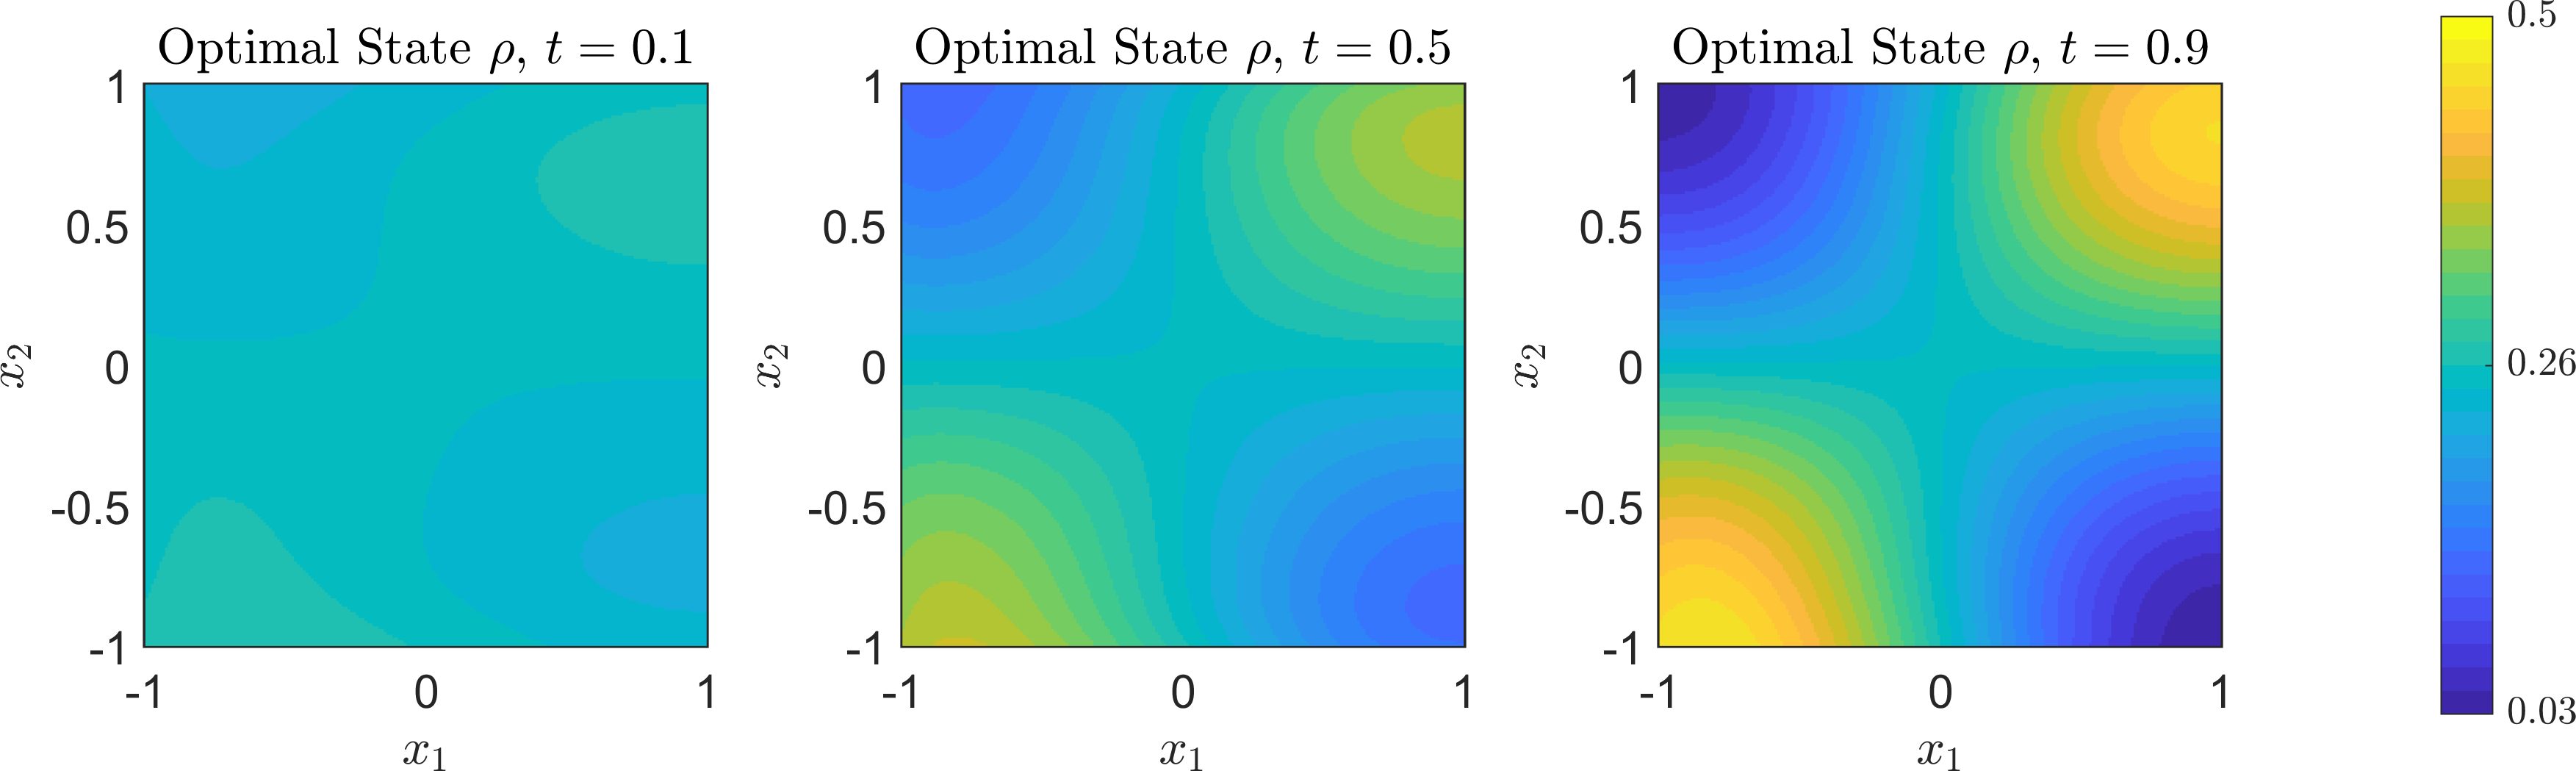
\includegraphics[scale=0.1]{SCNk0.png}
	\caption{Neumann Source Control: Optimal $\rho$ for $\kappa = 0$ and $\beta = 10^{-3}$.} 
	\label{FSCN1}
\end{figure}
\begin{figure}[h]
	\centering
	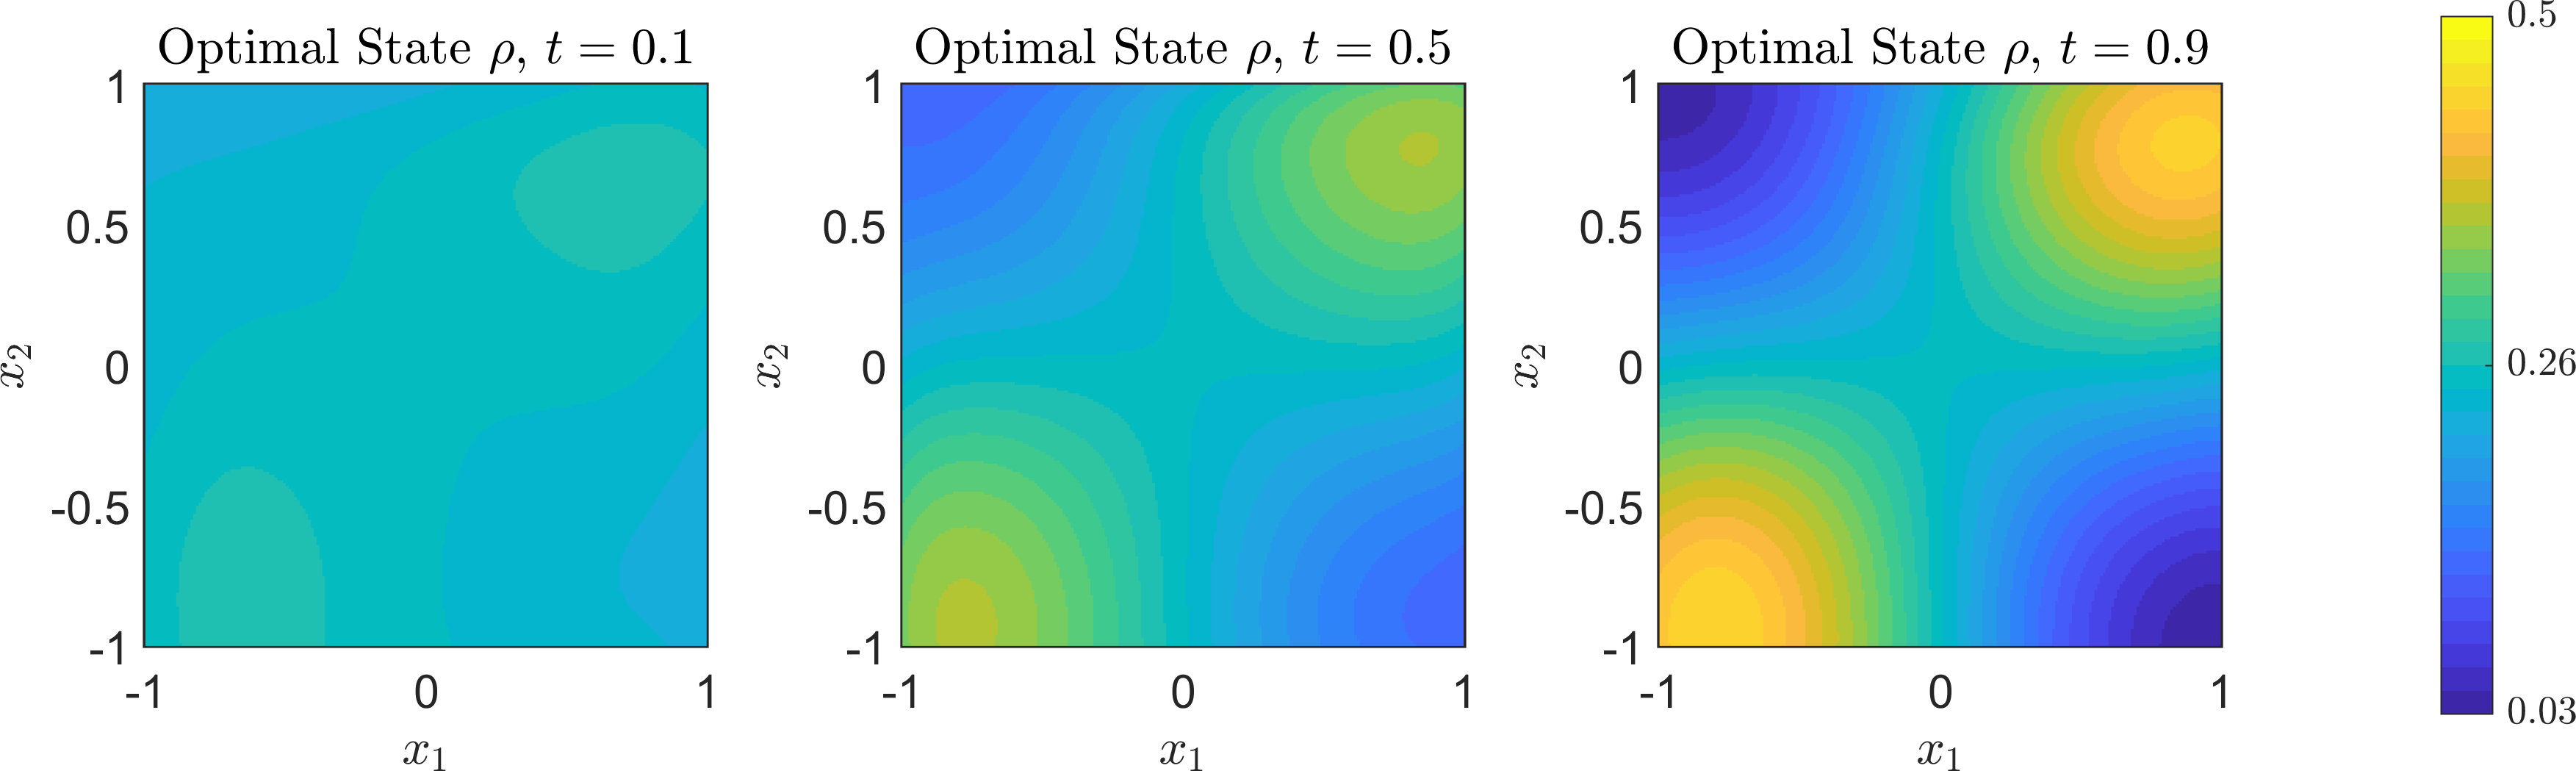
\includegraphics[scale=0.1]{SCNkn1.png}
	\caption{Neumann Source Control: Optimal $\rho$ for $\kappa = -1$ and $\beta = 10^{-3}$.} 
	\label{FSCN2}
\end{figure}
\begin{figure}[h]
	\centering
	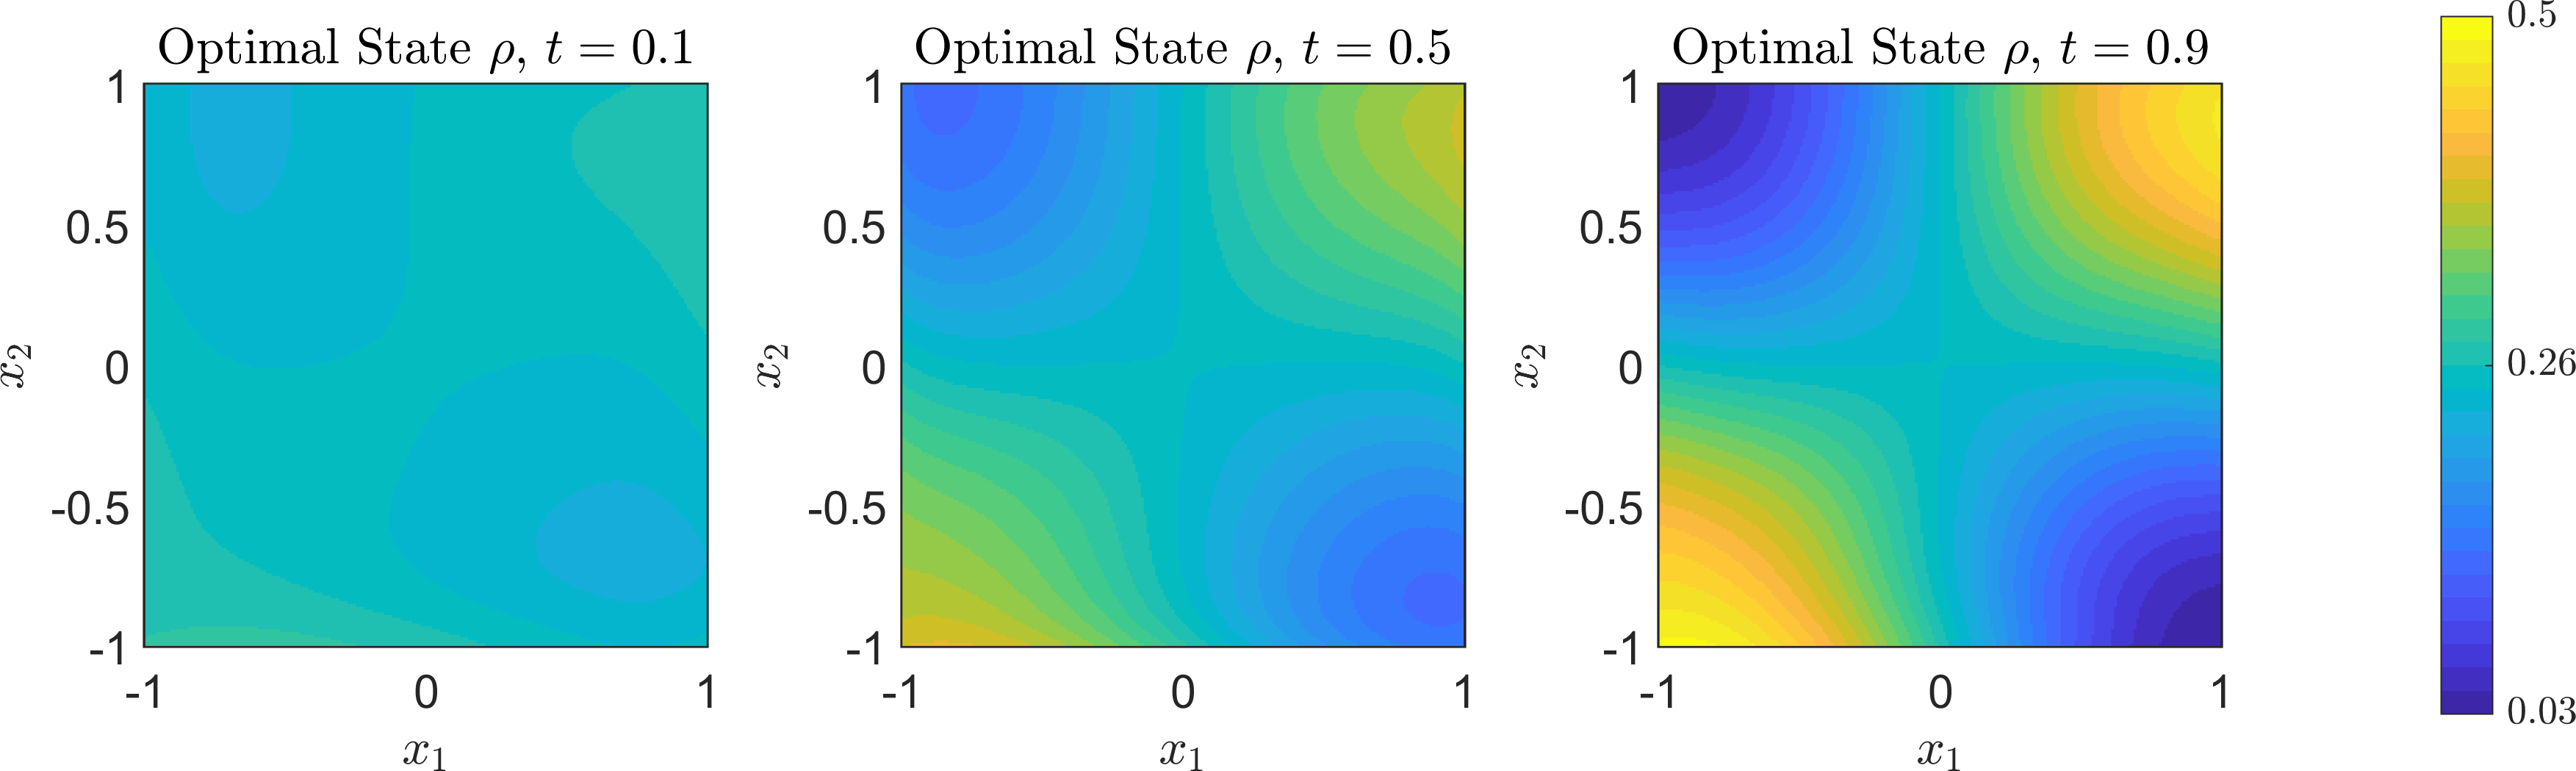
\includegraphics[scale=0.1]{SCNk1.png}
	\caption{Neumann Source Control: Optimal $\rho$ for $\kappa = 1$ and $\beta = 10^{-3}$.} 
	\label{FSCN3}
\end{figure}


\begin{figure}[h]
	\centering
	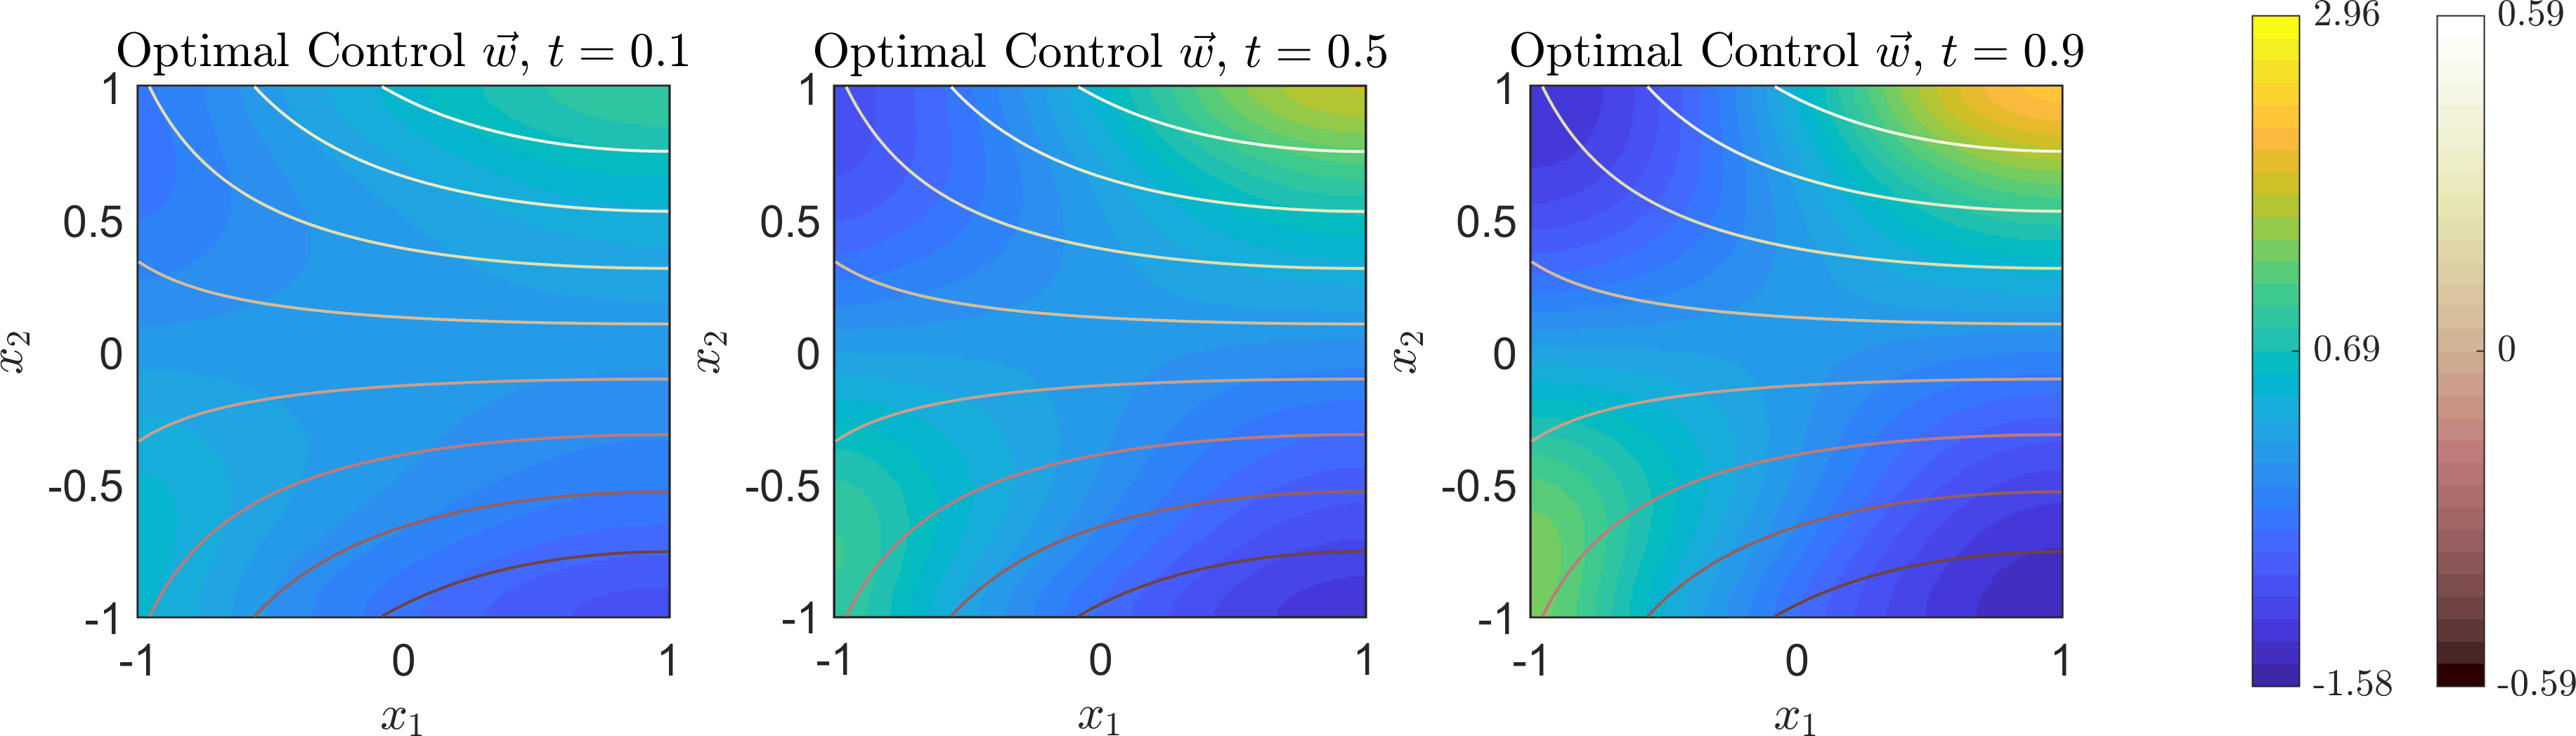
\includegraphics[scale=0.1]{SCNk0c.png}
	\caption{Neumann Source Control: Optimal control for $\kappa = 0$ and $\beta = 10^{-3}$. A contour plot of the external potential \emph{$V_{\text{ext}}$} is superimposed on the control plots for reference, with a corresponding colorbar on the left-hand side.} 
	\label{FSCN1c}
\end{figure}
\begin{figure}[h]
	\centering
	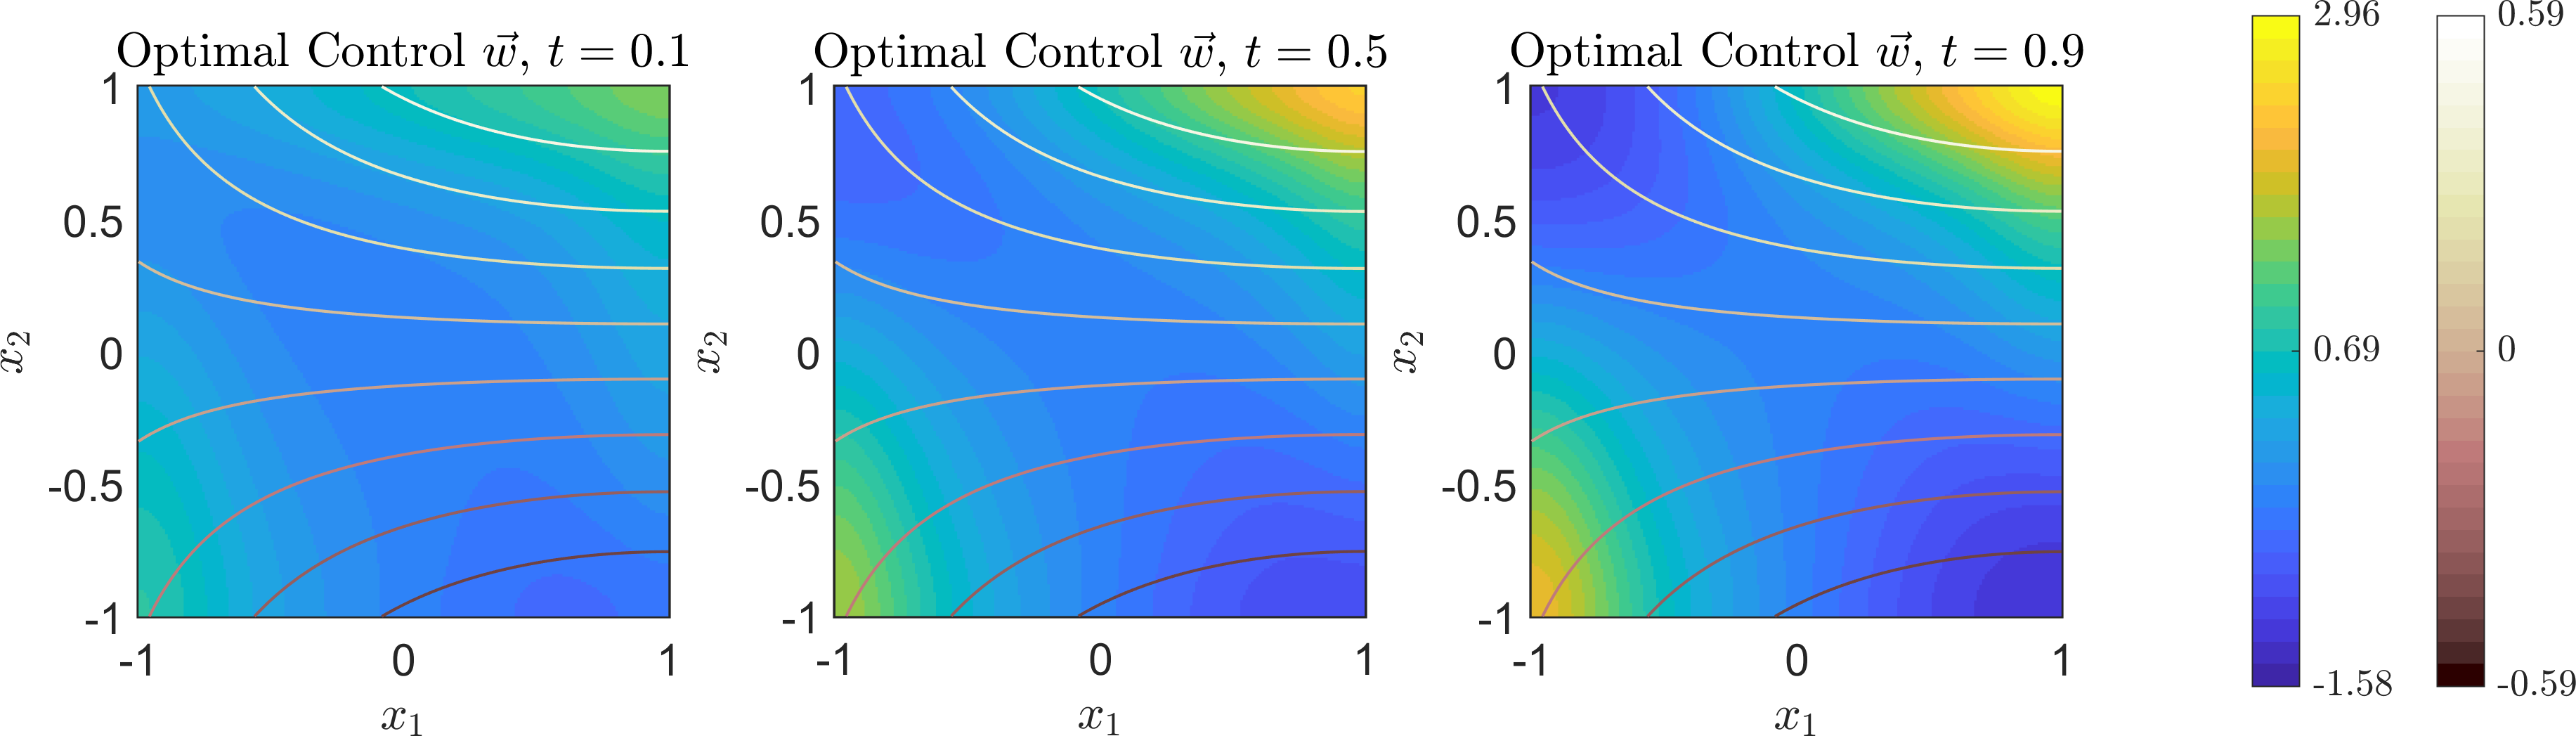
\includegraphics[scale=0.1]{SCNkn1c.png}
	\caption{Neumann Source Control: Optimal control for $\kappa = -1$ and $\beta = 10^{-3}$ and contour plot of the external potential \emph{$V_{\text{ext}}$} as before.} 
	\label{FSCN2c}
\end{figure}
\begin{figure}[h]
	\centering
	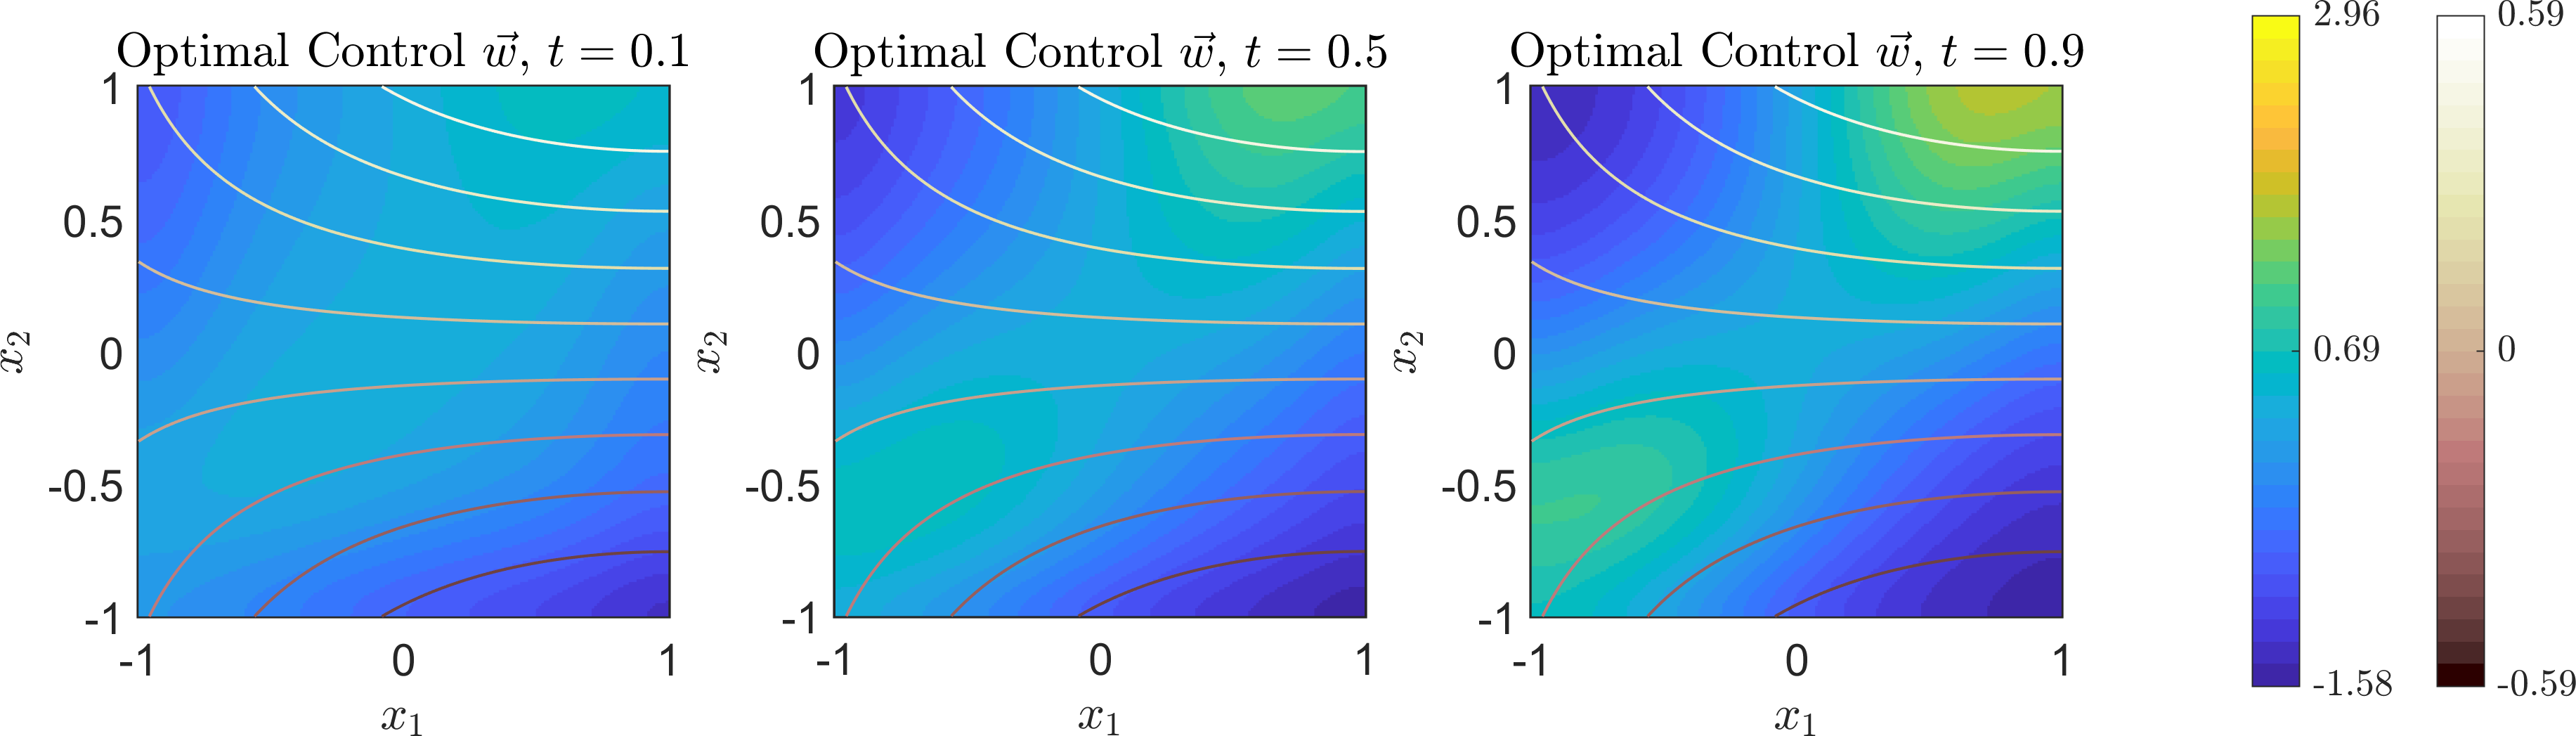
\includegraphics[scale=0.1]{SCNk1c.png}
	\caption{Neumann Source Control: Optimal control for $\kappa = 1$ and $\beta = 10^{-3}$ and contour plot of the external potential \emph{$V_{\text{ext}}$} as before.} 
	\label{FSCN3c}
\end{figure}


\subsubsection{Linear (source) control problem with Dirichlet boundary conditions}
We consider problem \eqref{AdvDiff_Linear} with Dirichlet boundary conditions \eqref{Dirichlet}.
The chosen inputs for our next example are:
\begin{align*}
	\rho_0 &= \frac{1}{4}\cos\left(\frac{\pi x_1}{2}\right)\cos\left(\frac{\pi x_2}{2}\right) + \frac{1}{4}, \quad V_{ext} =  \frac{3}{4}(1-t)\left(-\cos\left(\frac{\pi x_1}{2}\right)\sin\left(\frac{\pi x_2}{2}\right) + 1\right),\\
	\hr &= (1 - t)\left(\frac{1}{4}\cos\left(\frac{\pi x_1}{2}\right)\cos\left(\frac{\pi x_2}{2}\right) + \frac{1}{4}\right) - t\left(\frac{1}{4}\sin\left(\pi x_1\right)\sin\left(\frac{\pi x_2}{2} - \frac{\pi}{2}\right) + \frac{1}{4}\right).
\end{align*}
In this example we choose an external potential, which decays with time. This results in the strongest effect of $V_{ext}$ being visible at earlier times, and none at the final time. Since the external potential is steep around the bottom half of the domain, the mass of particles is not centred in the middle of the domain, but slightly shifted upward. At the same time it can be observed that at $t= 0.1$, the control is applied where the external potential is steep. At later times, the control is mostly applied where the particles are prescribed to accumulate by the desired state $\hr$, which is at the left half of the domain.
When comparing Figure \ref{F2b} displaying results for attractive particles, and Figure \ref{F2c}, showing the effect of repulsive particles, it is evident that the attractive particles cluster more, and therefore less control is needed to achieve the optimal state. The optimal controls corresponding to this are shown in Figures \ref{F2ac}, \ref{F2bc} and \ref{F2cc}.
The results can be seen in Table \ref{TabSCD}.

\begin{table}
\centering
\begin{tabular}{ | c | c || c | c | c | c | c ||}
\hline
\multicolumn{2}{|c||}{}& $\beta = 10^{-5}$ & $\beta = 10^{-3}$ & $\beta = 10^{-1}$ & $\beta = 10^{1}$ & $\beta = 10^{3}$  \\
\hline
\hline
\multirow{2}{*}{$\kappa= \numprint{0}$}  & $\mathcal{J}_{uc}$ & $\numprint{1.50e-2}$ & $\numprint{1.50e-2}$ & $\numprint{1.50e-2}$ & $\numprint{1.50e-2}$ & $\numprint{1.50e-2}$\\
 & $\mathcal{J}_c$ & $\numprint{3.40e-5}$ & $\numprint{1.92e-3}$ & $\numprint{1.36e-2}$ & $\numprint{1.50e-2}$ & $\numprint{1.50e-2}$\\
\hline
\multirow{2}{*}{$\kappa= \numprint{1}$}  & $\mathcal{J}_{uc}$ & $\numprint{2.06e-2}$ & $\numprint{2.06e-2}$ & $\numprint{2.06e-2}$ & $\numprint{2.06e-2}$ & $\numprint{2.06e-2}$\\
 & $\mathcal{J}_c$ & $\numprint{4.27e-5}$ & $\numprint{2.49e-3}$ & $\numprint{1.85e-2}$ & $\numprint{2.06e-2}$ & $\numprint{2.06e-2}$\\
\hline
\multirow{2}{*}{$\kappa= \numprint{-1}$}  & $\mathcal{J}_{uc}$ & $\numprint{1.27e-2}$ & $\numprint{1.27e-2}$ & $\numprint{1.27e-2}$ & $\numprint{1.27e-2}$ & $\numprint{1.27e-2}$\\
 & $\mathcal{J}_c$ & $\numprint{2.88e-5}$ & $\numprint{1.61e-3}$ & $\numprint{1.18e-2}$ & $\numprint{1.27e-2}$ & $\numprint{1.27e-2}$\\
\hline
\end{tabular}
\caption{Source Control Dirichlet Problem: Cost $\mathcal{J}_{uc}$ of applying no control (i.e., $\vec{w} = \vec{0}$)and optimal control cost $\mathcal{J}_{c}$ for a range of values of the interaction strength $\kappa$ and regularization parameter $\beta$. The value of $\mathcal J_{c}$ for $\beta = 10^{-5}$ is of order $10^{-5}$. Note that for $\beta = 10$, the cost functionals differ by $10{-5}$, while for $\beta = 10^3$ they differ by $10^{-7}$ for $\kappa = 0$ and $\kappa = 1$ and by $10^{-8}$ for $\kappa = -1$.}
\label{TabSCD}
\end{table}
\begin{figure}[h]
	\centering
	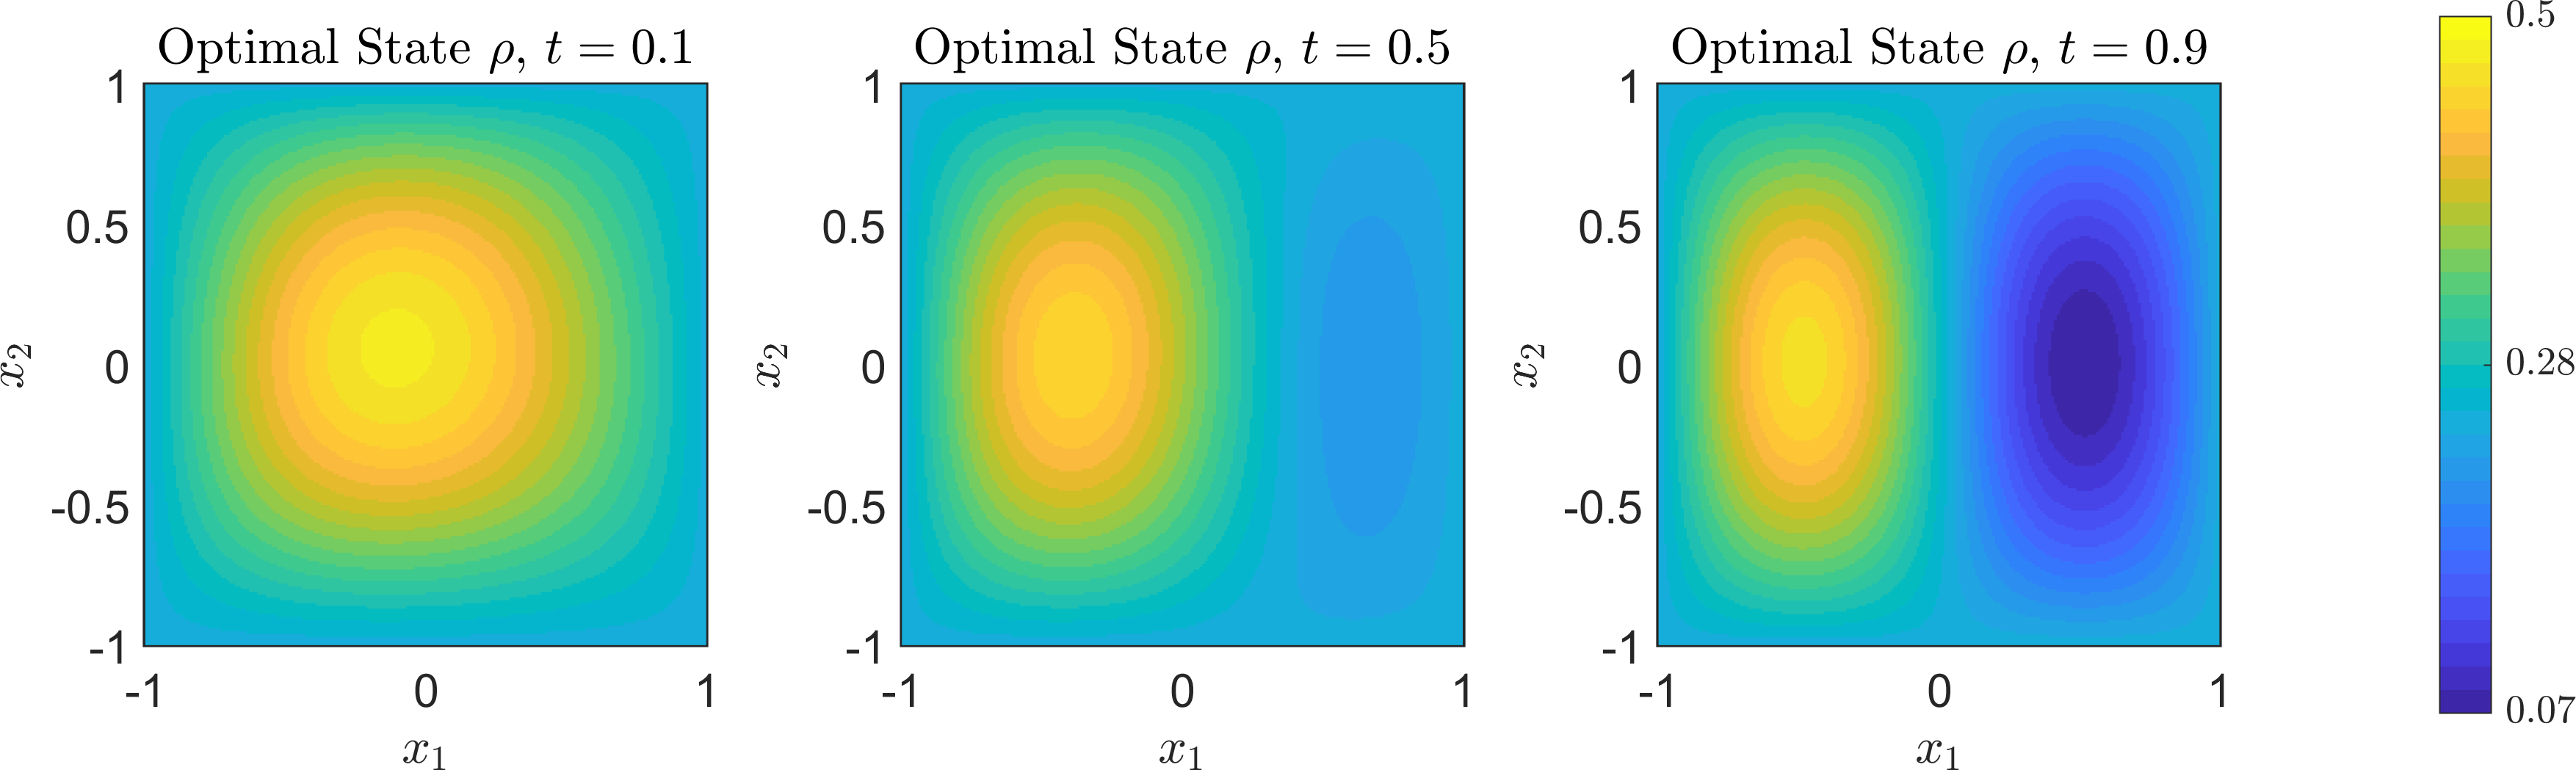
\includegraphics[scale=0.1]{SCDk0.png}
	\caption{Dirichlet Source Control: Optimal $\rho$ for $\kappa = 0$ and $\beta = 10^{-3}$.} 
	\label{F2a}
\end{figure}
\begin{figure}[h]
	\centering
	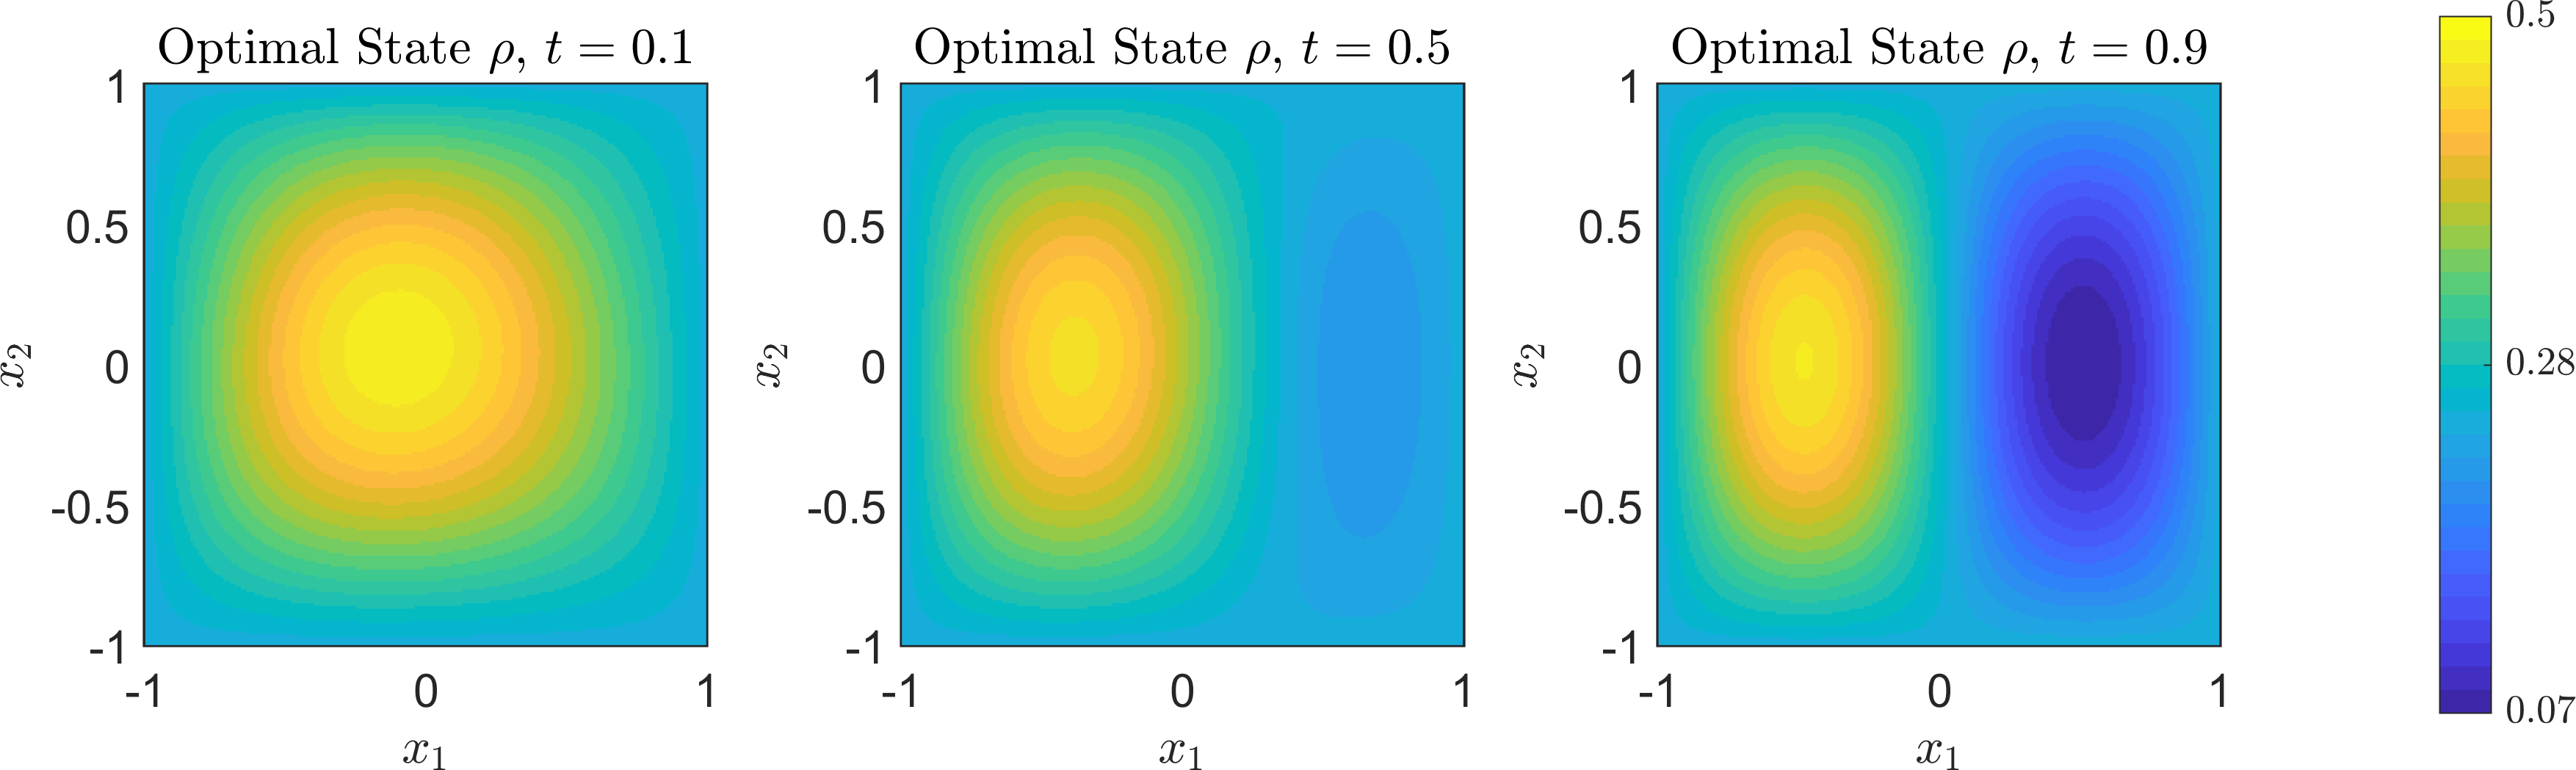
\includegraphics[scale=0.1]{SCDkn1.png}
	\caption{Dirichlet Source Control: Optimal $\rho$ for $\kappa = -1$ and $\beta = 10^{-3}$.} 
	\label{F2b}
\end{figure}
\begin{figure}[h]
	\centering
	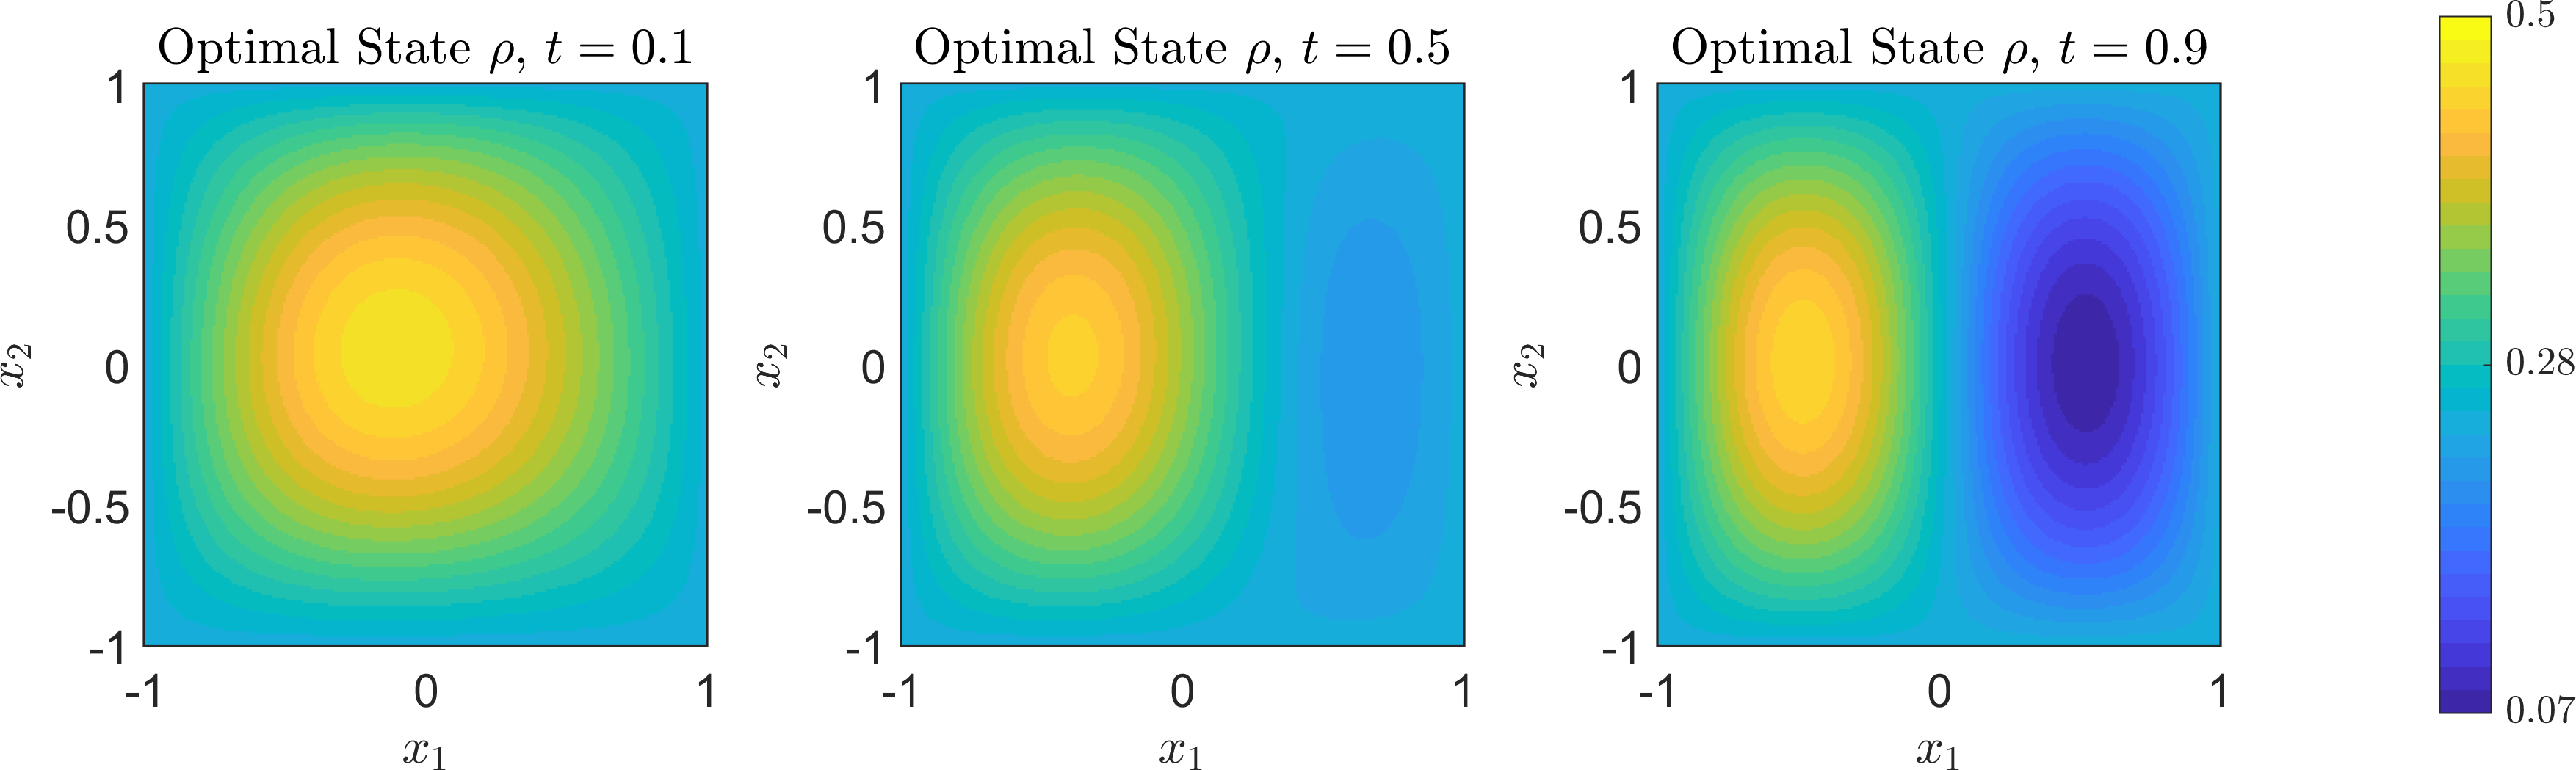
\includegraphics[scale=0.1]{SCDk1.png}
	\caption{Dirichlet Source Control: Optimal $\rho$ for $\kappa = 1$ and $\beta = 10^{-3}$.} 
	\label{F2c}
\end{figure}

	\begin{figure}[h]
	\centering
	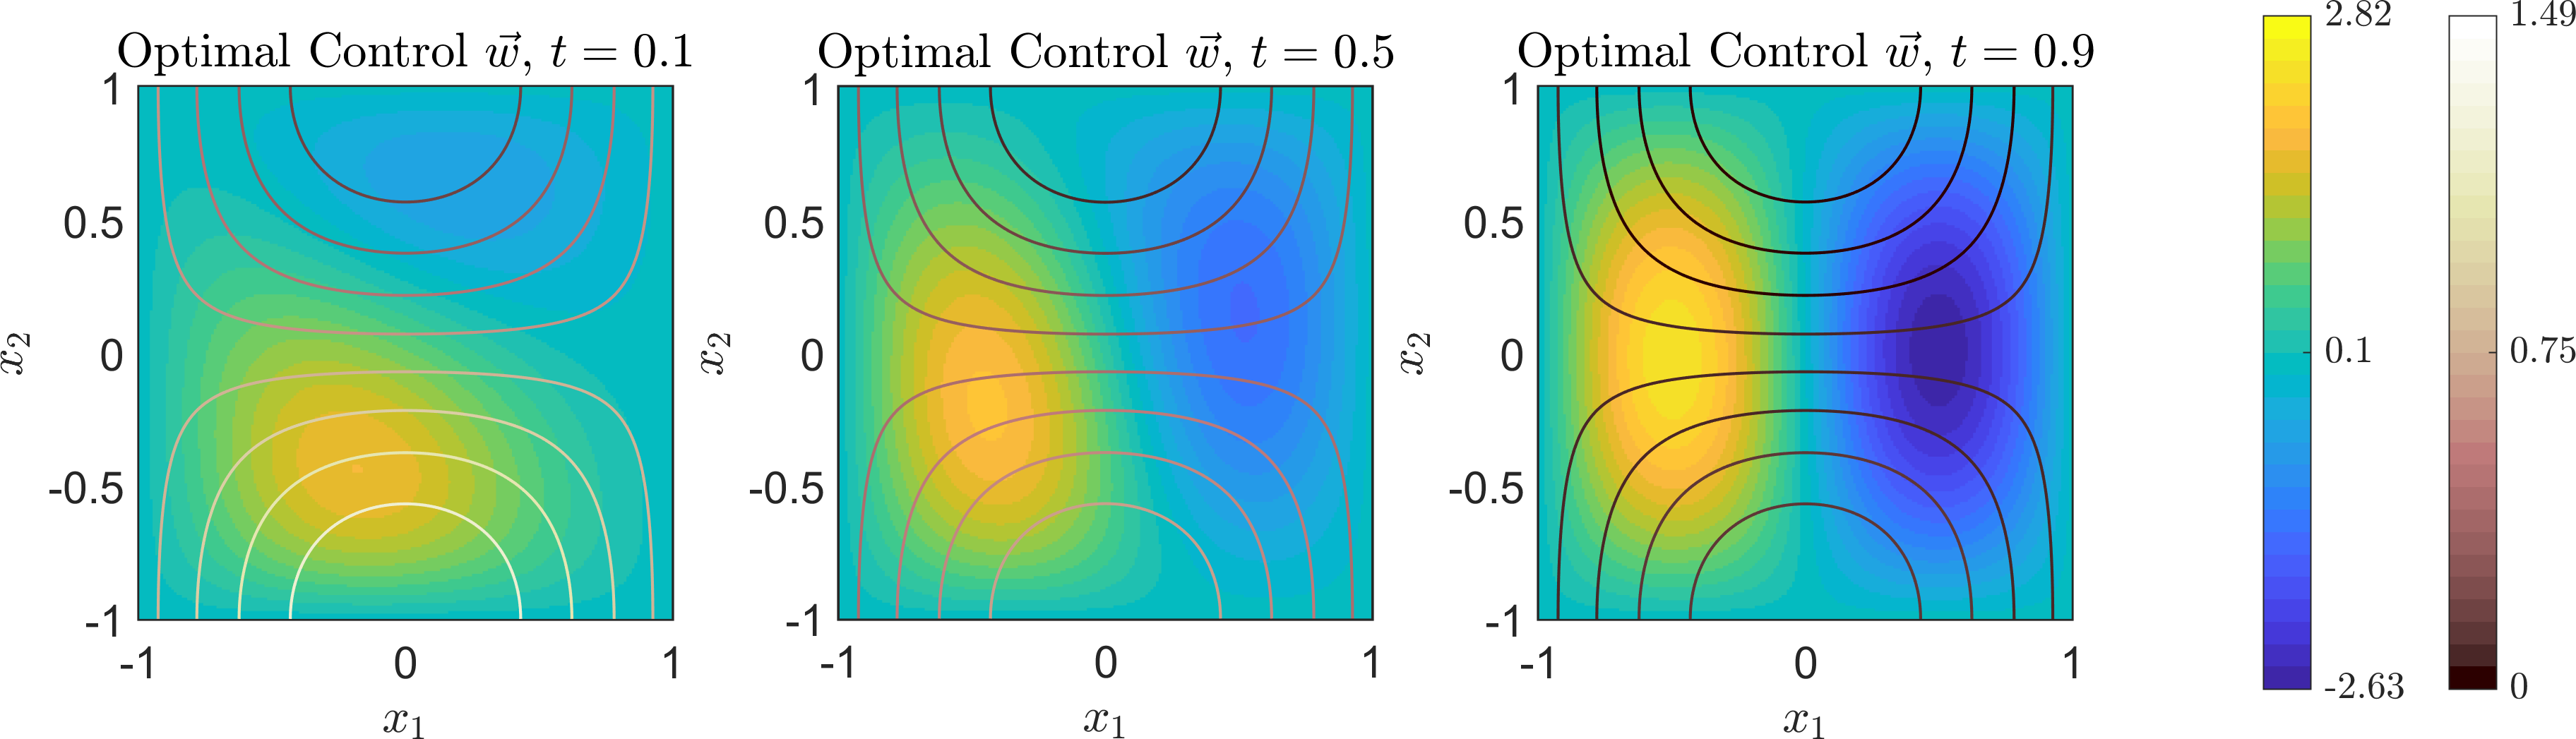
\includegraphics[scale=0.1]{SCDk0c.png}
	\caption{Dirichlet Source Control: Optimal control for $\kappa = 0$ and $\beta = 10^{-3}$. A contour plot of the external potential \emph{$V_{\text{ext}}$} is superimposed on the control plots for reference, with a corresponding colorbar on the left-hand side.} 
	\label{F2ac}
\end{figure}
\begin{figure}[h]
	\centering
	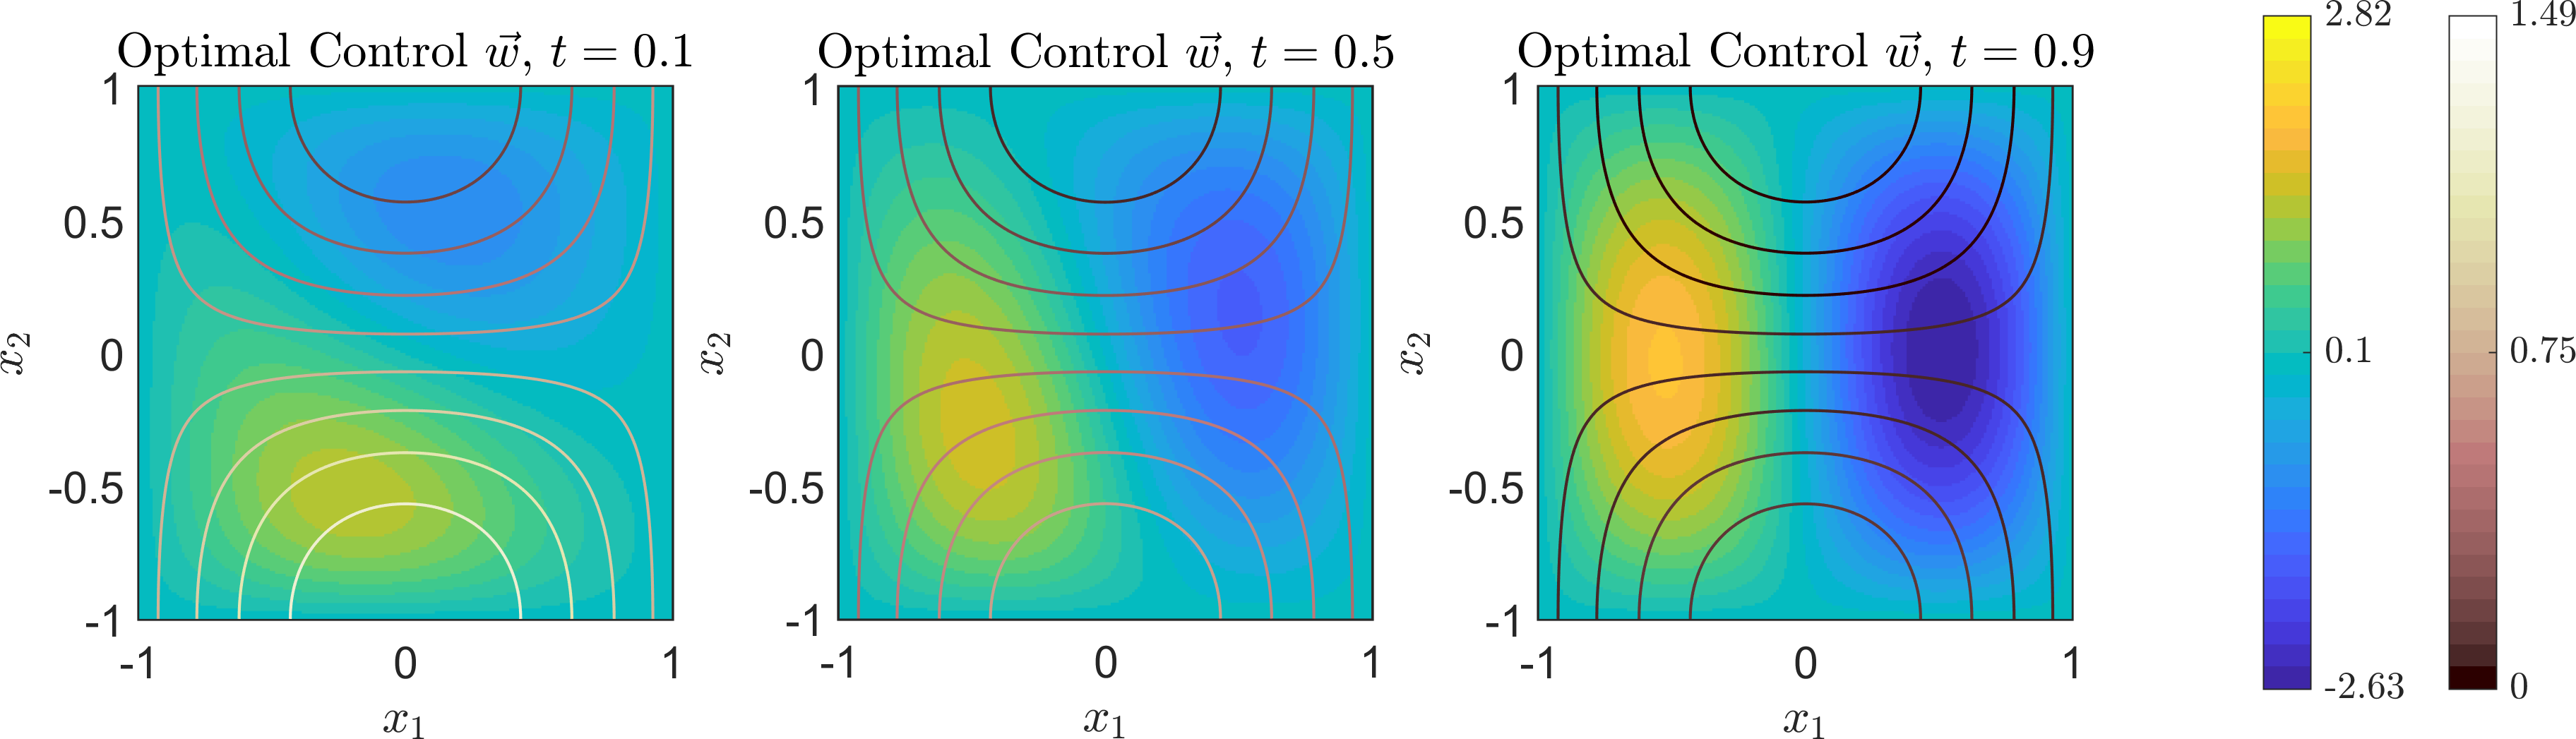
\includegraphics[scale=0.1]{SCDkn1c.png}
	\caption{Dirichlet Source Control: Optimal control for $\kappa = -1$ and $\beta = 10^{-3}$ and contour plot of the external potential \emph{$V_{\text{ext}}$} as before.} 
	\label{F2bc}
\end{figure}
\begin{figure}[h]
	\centering
	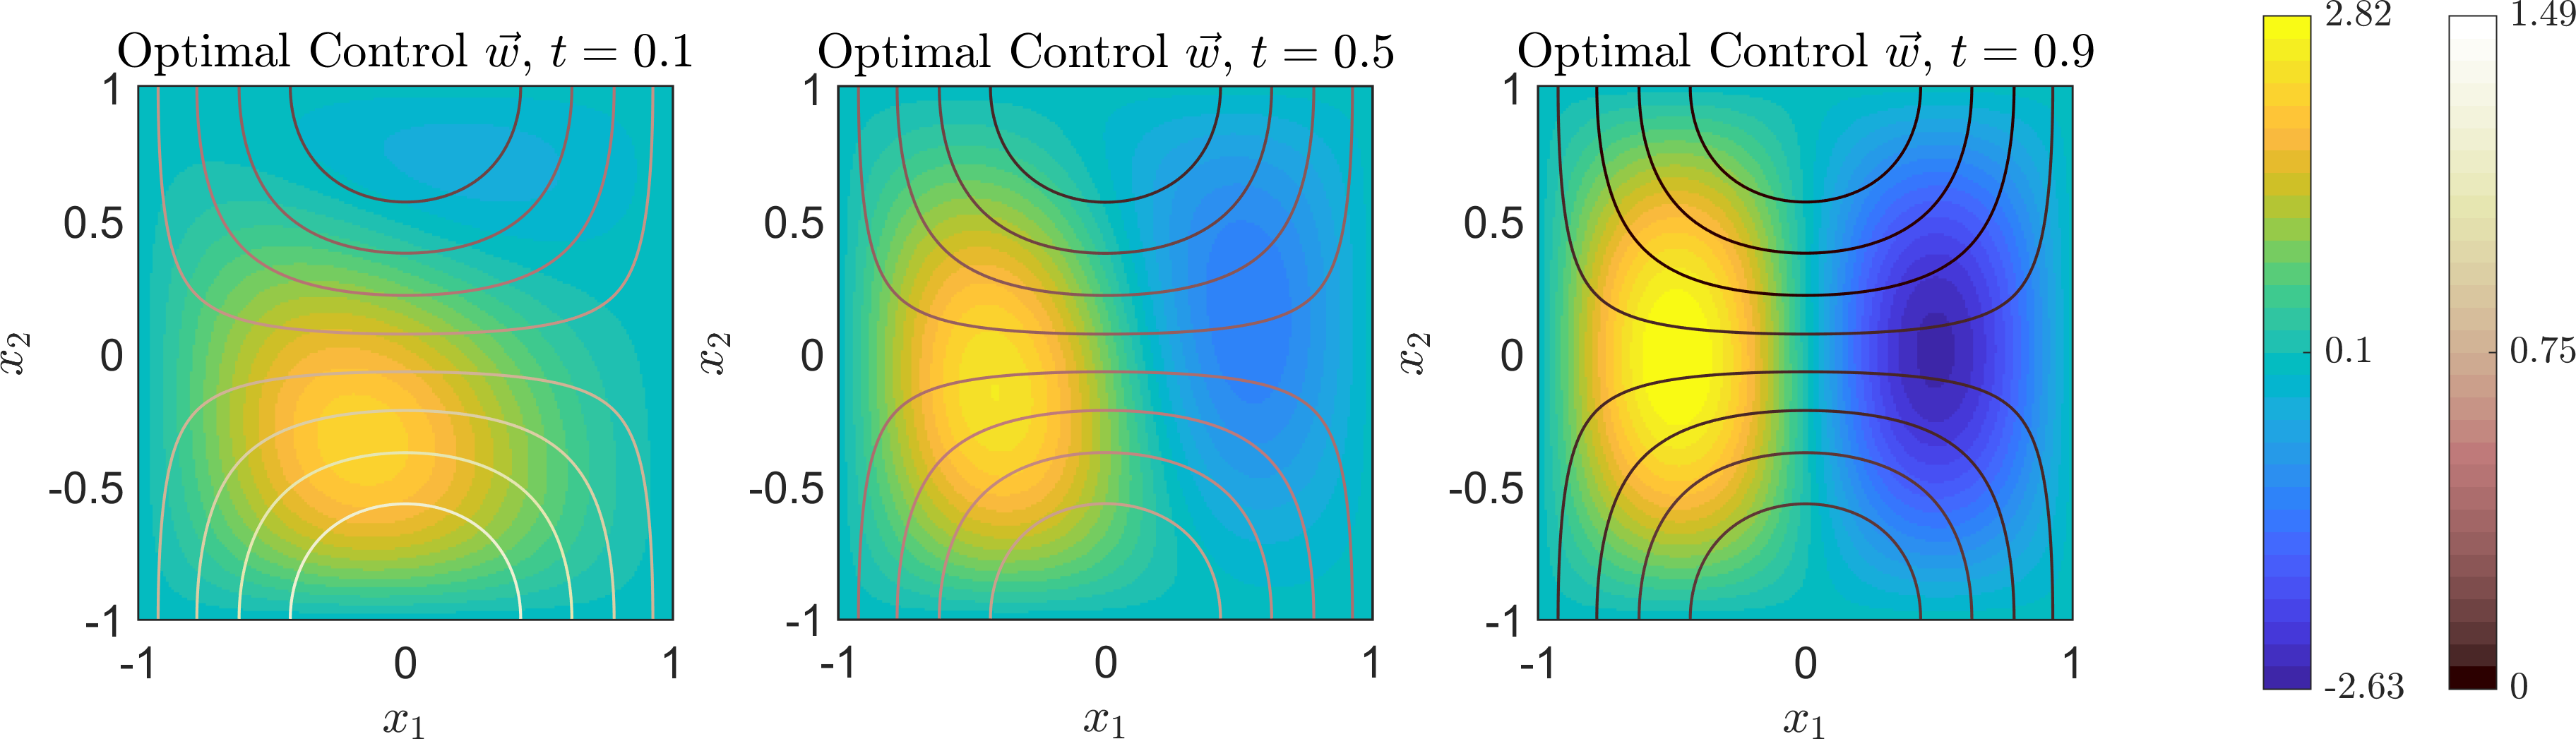
\includegraphics[scale=0.1]{SCDk1c.png}
	\caption{Dirichlet Source Control: Optimal control for $\kappa = 1$ and $\beta = 10^{-3}$ and contour plot of the external potential \emph{$V_{\text{ext}}$} as before.} 
	\label{F2cc}
\end{figure}



\subsubsection{Non-linear (flow) control problem with no-flux boundary conditions}
Next an example of system \eqref{AdvDiff} is considered with no-flux boundary conditions \eqref{NoFlux}.
The inputs here are:
\begin{align*}
	\rho_0 &= \frac{1}{4}, \quad \hr = \frac{1}{4}(1-t) + t\frac{1}{1.3791}\exp{\left(-2\left(\left(x_1+0.2\right)^2 + \left(x_2+0.2\right)^2\right)\right)},\\
	V_{ext} &= \left(\left(x_1 + 0.3\right)^2 - 1\right)\left(\left(x_1-0.4\right)^2 - 0.5\right)
	\left(\left(x_2 + 0.3\right)^2 - 1\right)\left(\left(x_2-0.4\right)^2 - 0.5\right).
\end{align*}
The numerical results for this example are displayed in Table \ref{TabFCN}. The results are illustrated for $\beta = 10^{-3}$ and $\kappa = -1$. Figures \ref{F3a}, \ref{F3b} and \ref{F3c} demonstrate the effect of $V_{\text{ext}}$ on the state, while Figures \ref{F3ac}, \ref{F3bc} and \ref{F3cc} display the corresponding controls. At earlier times, the particle mass accumulates in regions with potential wells and the areas where the potential is steep are avoided. In the Figures it can be observed very clearly that the control is driving the particle distribution to the desired state. It is noticeable that the control does not act uniformly around the peak of the desired state, but also acts strongly in the area between the location of the desired peak and the point $(-1,1)$. This is due to the external potential being steep in this area and more control is needed to reach the desired state than in other parts of the domain. 
((++ Comment on Cost update example! ++))

\begin{table}
\centering
\begin{tabular}{ | c | c || c | c | c | c | c ||}
\hline
\multicolumn{2}{|c||}{}& $\beta = 10^{-5}$ & $\beta = 10^{-3}$ & $\beta = 10^{-1}$ & $\beta = 10^{1}$ & $\beta = 10^{3}$  \\
\hline
\hline
\multirow{2}{*}{$\kappa= \numprint{0}$}  & $\mathcal{J}_{uc}$ & $\numprint{2.67e-2}$ & $\numprint{2.67e-2}$ & $\numprint{2.67e-2}$ & $\numprint{2.67e-2}$ & $\numprint{2.67e-2}$\\
 & $\mathcal{J}_c$ & $\numprint{8.23e-5}$ & $\numprint{3.87e-3}$ & $\numprint{2.50e-2}$ & $\numprint{2.67e-2}$ & $\numprint{2.67e-2}$\\
\hline
\multirow{2}{*}{$\kappa= \numprint{1}$}  & $\mathcal{J}_{uc}$ & $\numprint{3.29e-2}$ & $\numprint{3.29e-2}$ & $\numprint{3.29e-2}$ & $\numprint{3.29e-2}$ & $\numprint{3.29e-2}$\\
 & $\mathcal{J}_c$ & $\numprint{1.16e-4}$ & $\numprint{5.44e-3}$ & $\numprint{3.13e-2}$ & $\numprint{3.29e-2}$ & $\numprint{3.29e-2}$\\
\hline
\multirow{2}{*}{$\kappa= \numprint{-1}$}  & $\mathcal{J}_{uc}$ & $\numprint{2.09e-2}$ & $\numprint{2.09e-2}$ & $\numprint{2.09e-2}$ & $\numprint{2.09e-2}$ & $\numprint{2.09e-2}$\\
 & $\mathcal{J}_c$ & $\numprint{5.71e-5}$ & $\numprint{2.63e-3}$ & $\numprint{1.92e-2}$ & $\numprint{2.09e-2}$ & $\numprint{2.09e-2}$\\
\hline
\end{tabular}
\caption{Flow Control No-Flux Problem: Cost when $\vec{w}=\vec{0}$ and optimal control cost for a range of $\kappa$, $\beta$. Note that for $\beta = 10$, the cost functionals differ by $10^{-5}$, while for $\beta = 10^3$ they differ by $10^{-7}$ (++ two in the wrong direction ++).}
\label{TabFCN}
\end{table}
\begin{figure}[h]
	\centering
	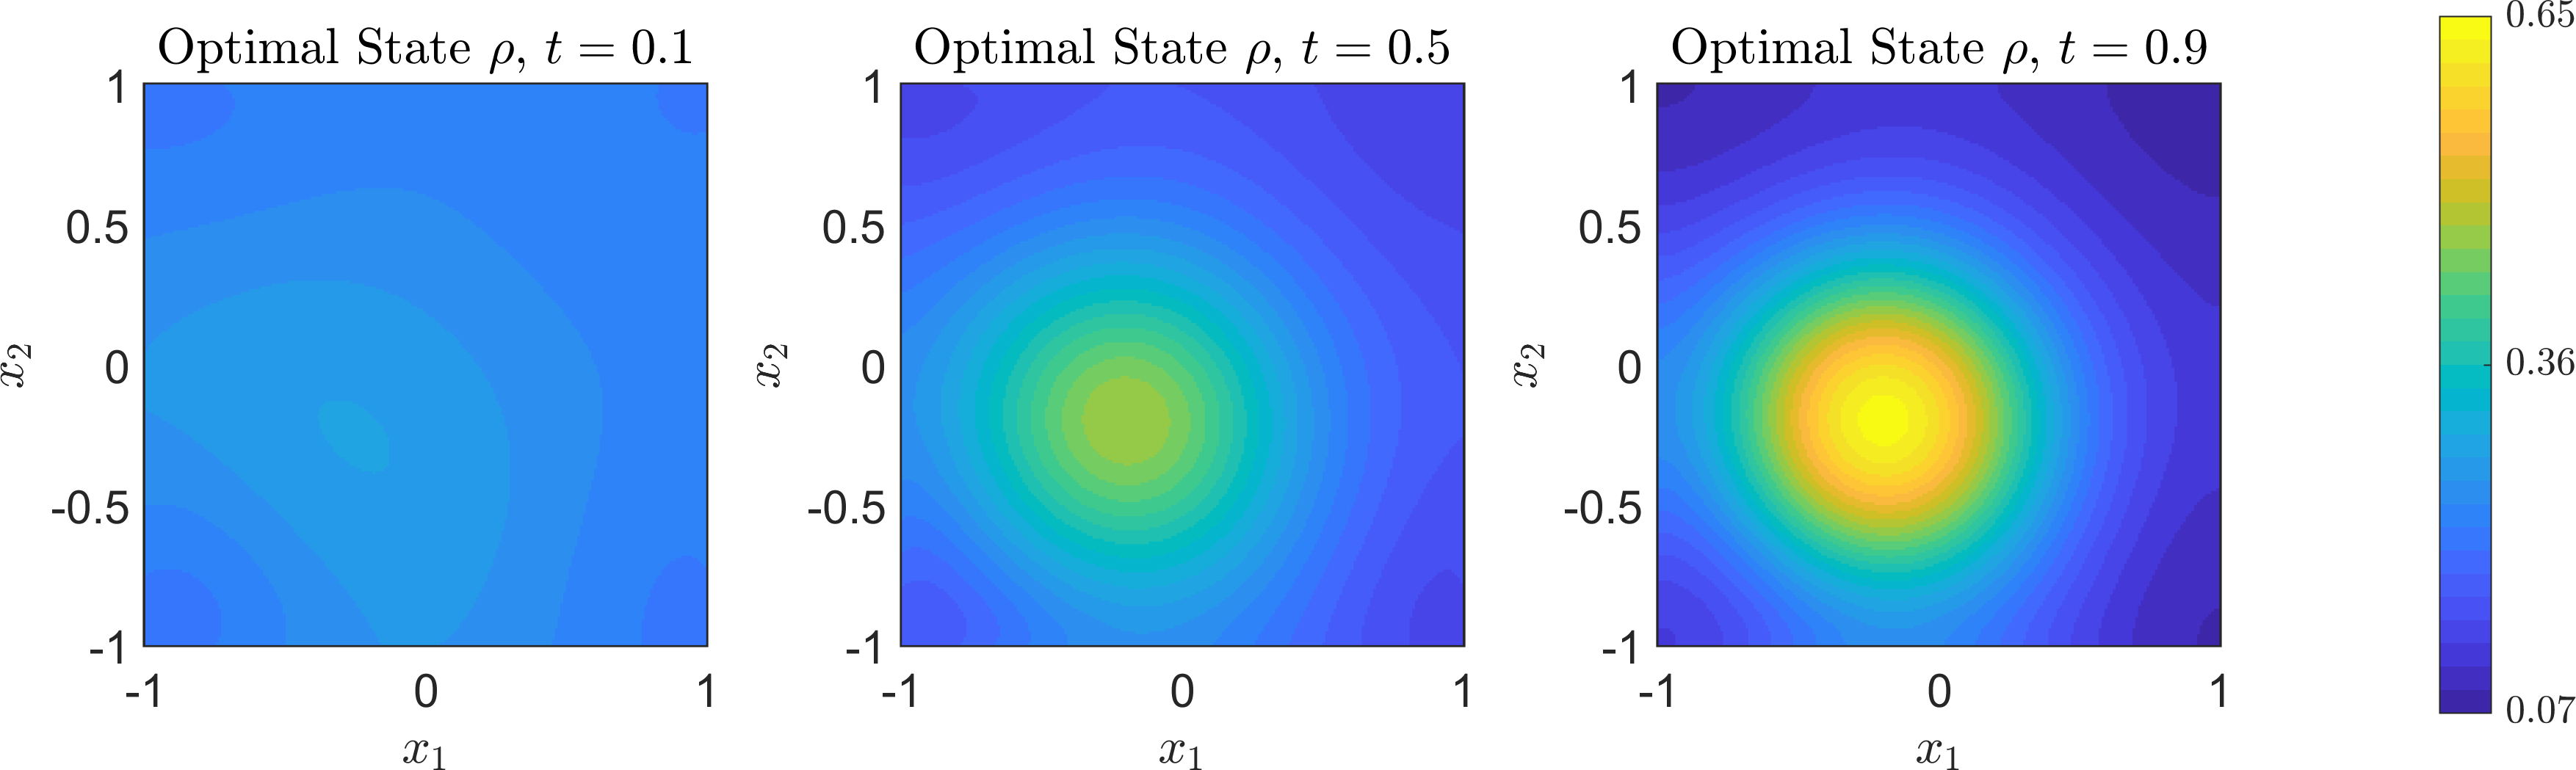
\includegraphics[scale=0.1]{FCNk0.png}
	\caption{Neumann Flow Control: Optimal $\rho$ for $\kappa = 0$ and $\beta = 10^{-3}$.} 
	\label{F3a}
\end{figure}
\begin{figure}[h]
	\centering
	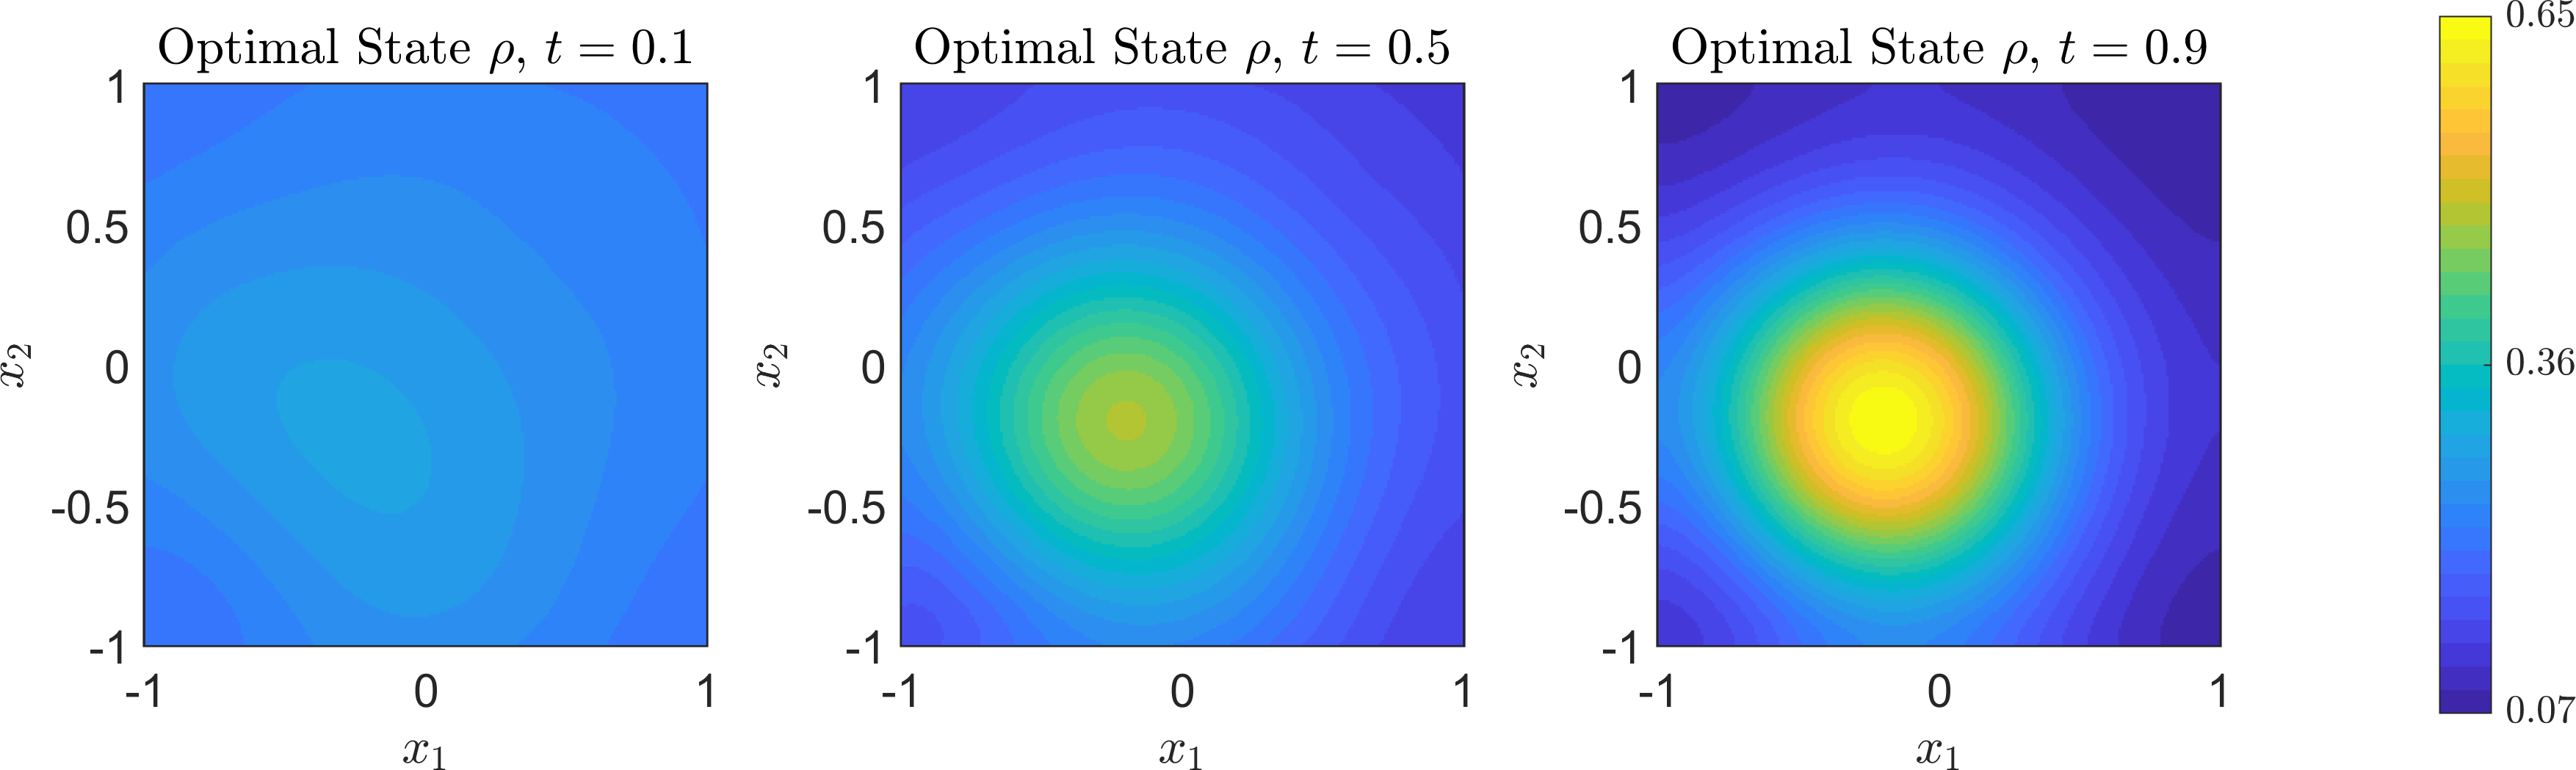
\includegraphics[scale=0.1]{FCNkn1.png}
	\caption{Neumann Flow Control: Optimal $\rho$ for $\kappa = -1$ and $\beta = 10^{-3}$.} 
	\label{F3b}
\end{figure}
\begin{figure}[h]
	\centering
	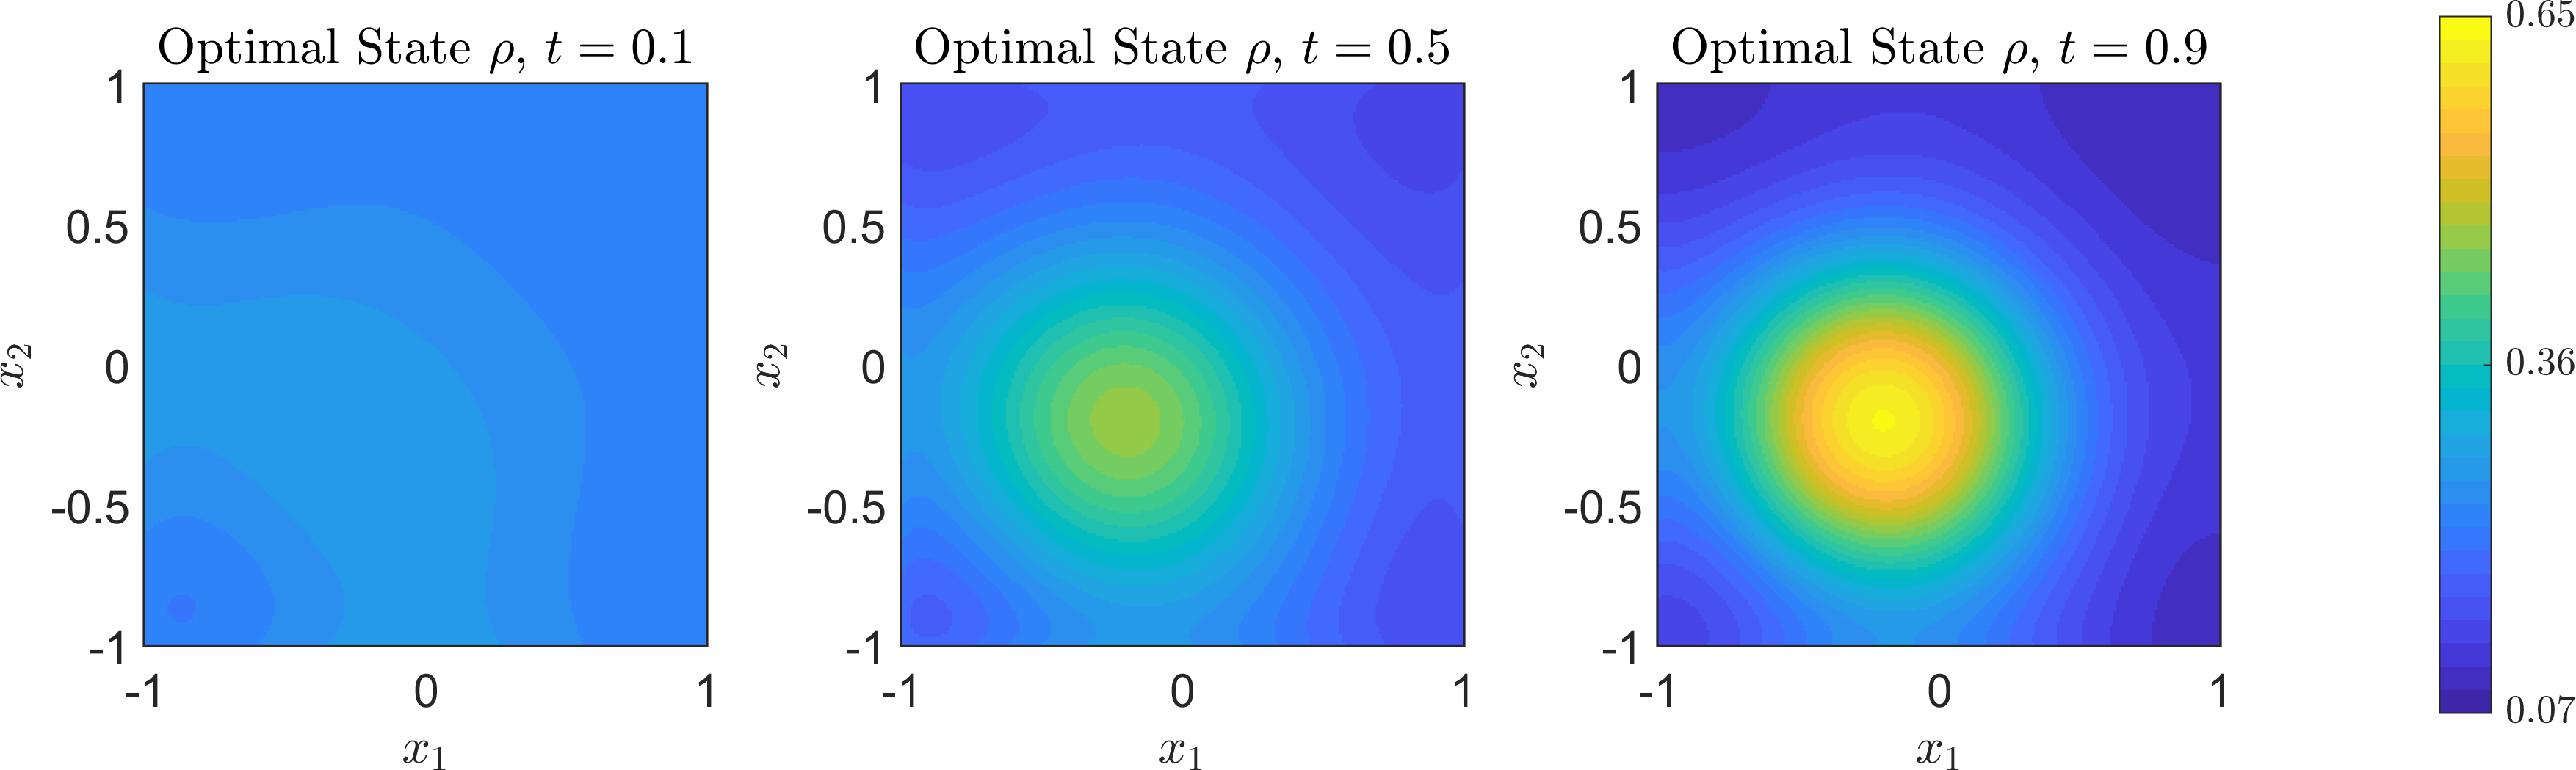
\includegraphics[scale=0.1]{FCNk1.png}
	\caption{Neumann Flow Control: Optimal $\rho$ for $\kappa = 1$ and $\beta = 10^{-3}$.} 
	\label{F3c}
\end{figure}


\begin{figure}[h]
	\centering
	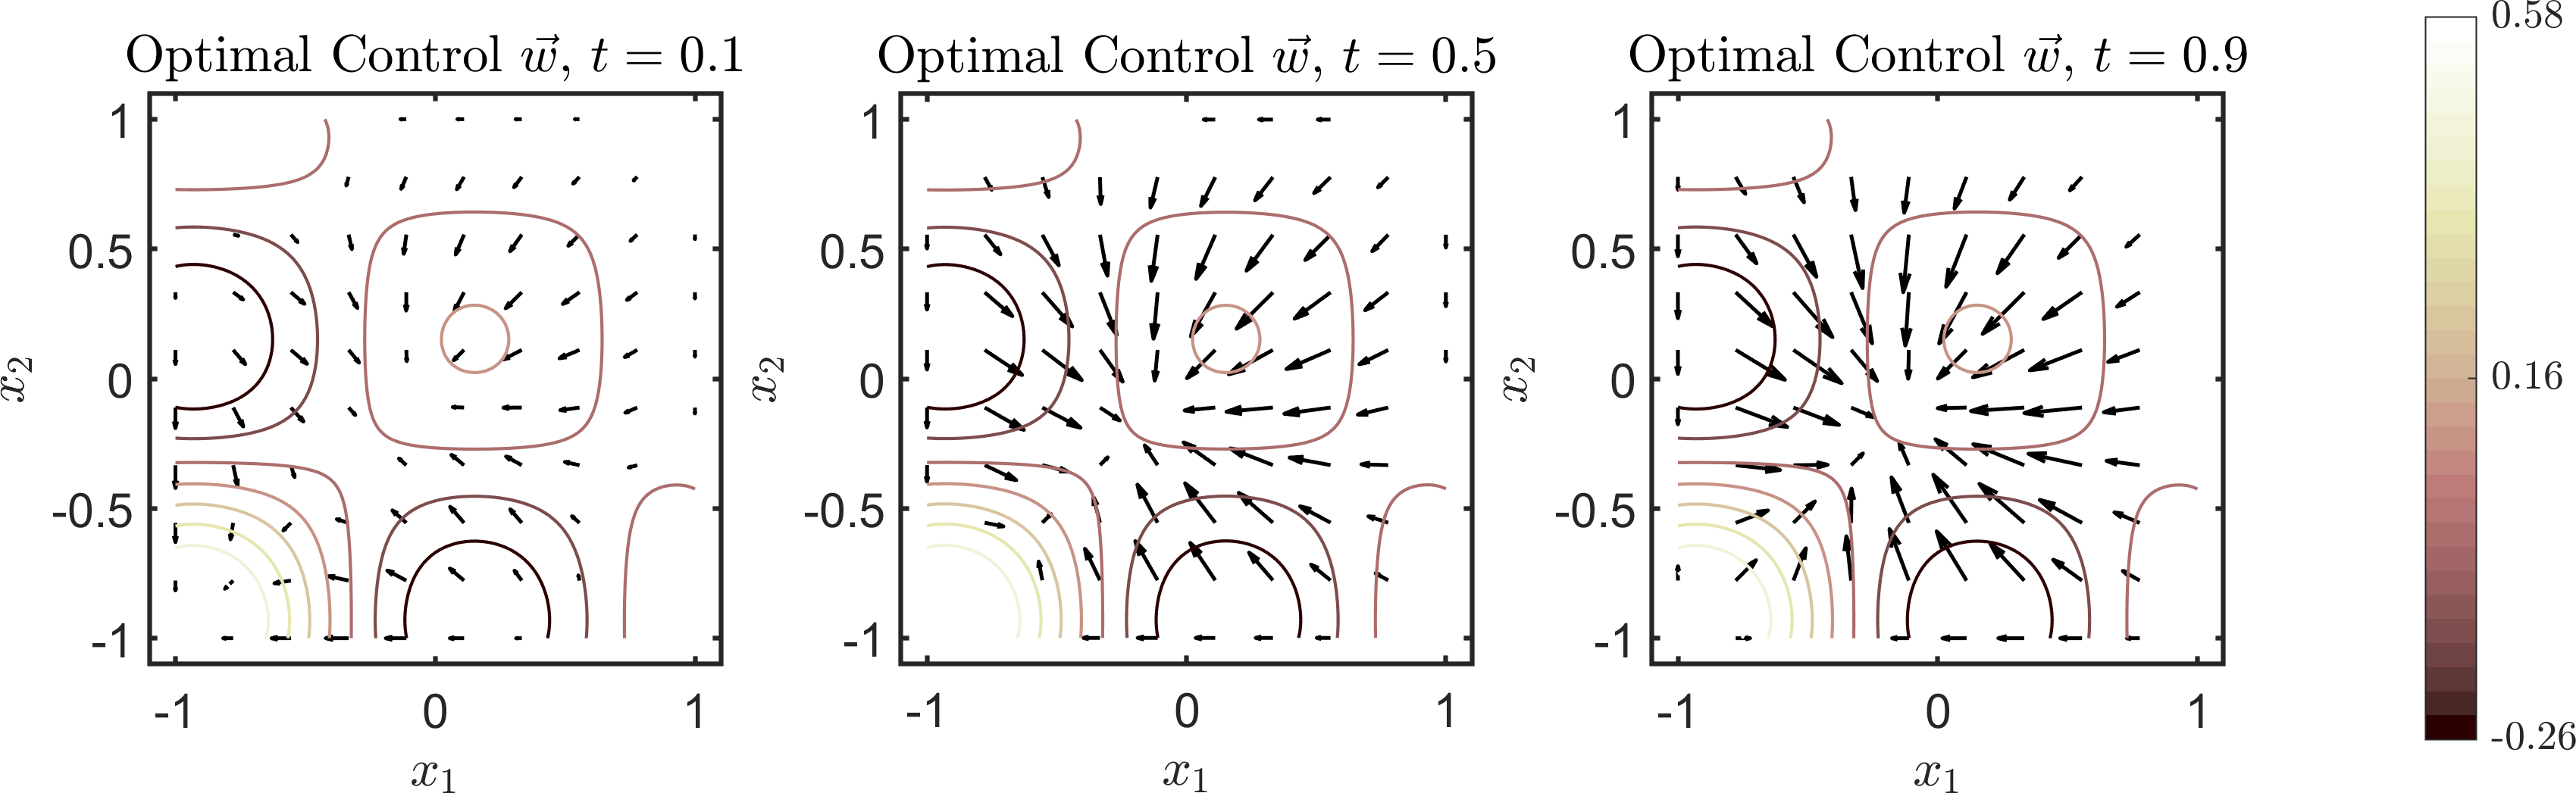
\includegraphics[scale=0.1]{FCNk0c.png}
	\caption{Neumann Flow Control: Optimal control for $\kappa = 0$ and $\beta = 10^{-3}$. A contour plot of the external potential \emph{$V_{\text{ext}}$} is superimposed on the control plots for reference, with a corresponding colorbar on the left-hand side.} 
	\label{F3ac}
\end{figure}
\begin{figure}[h]
	\centering
	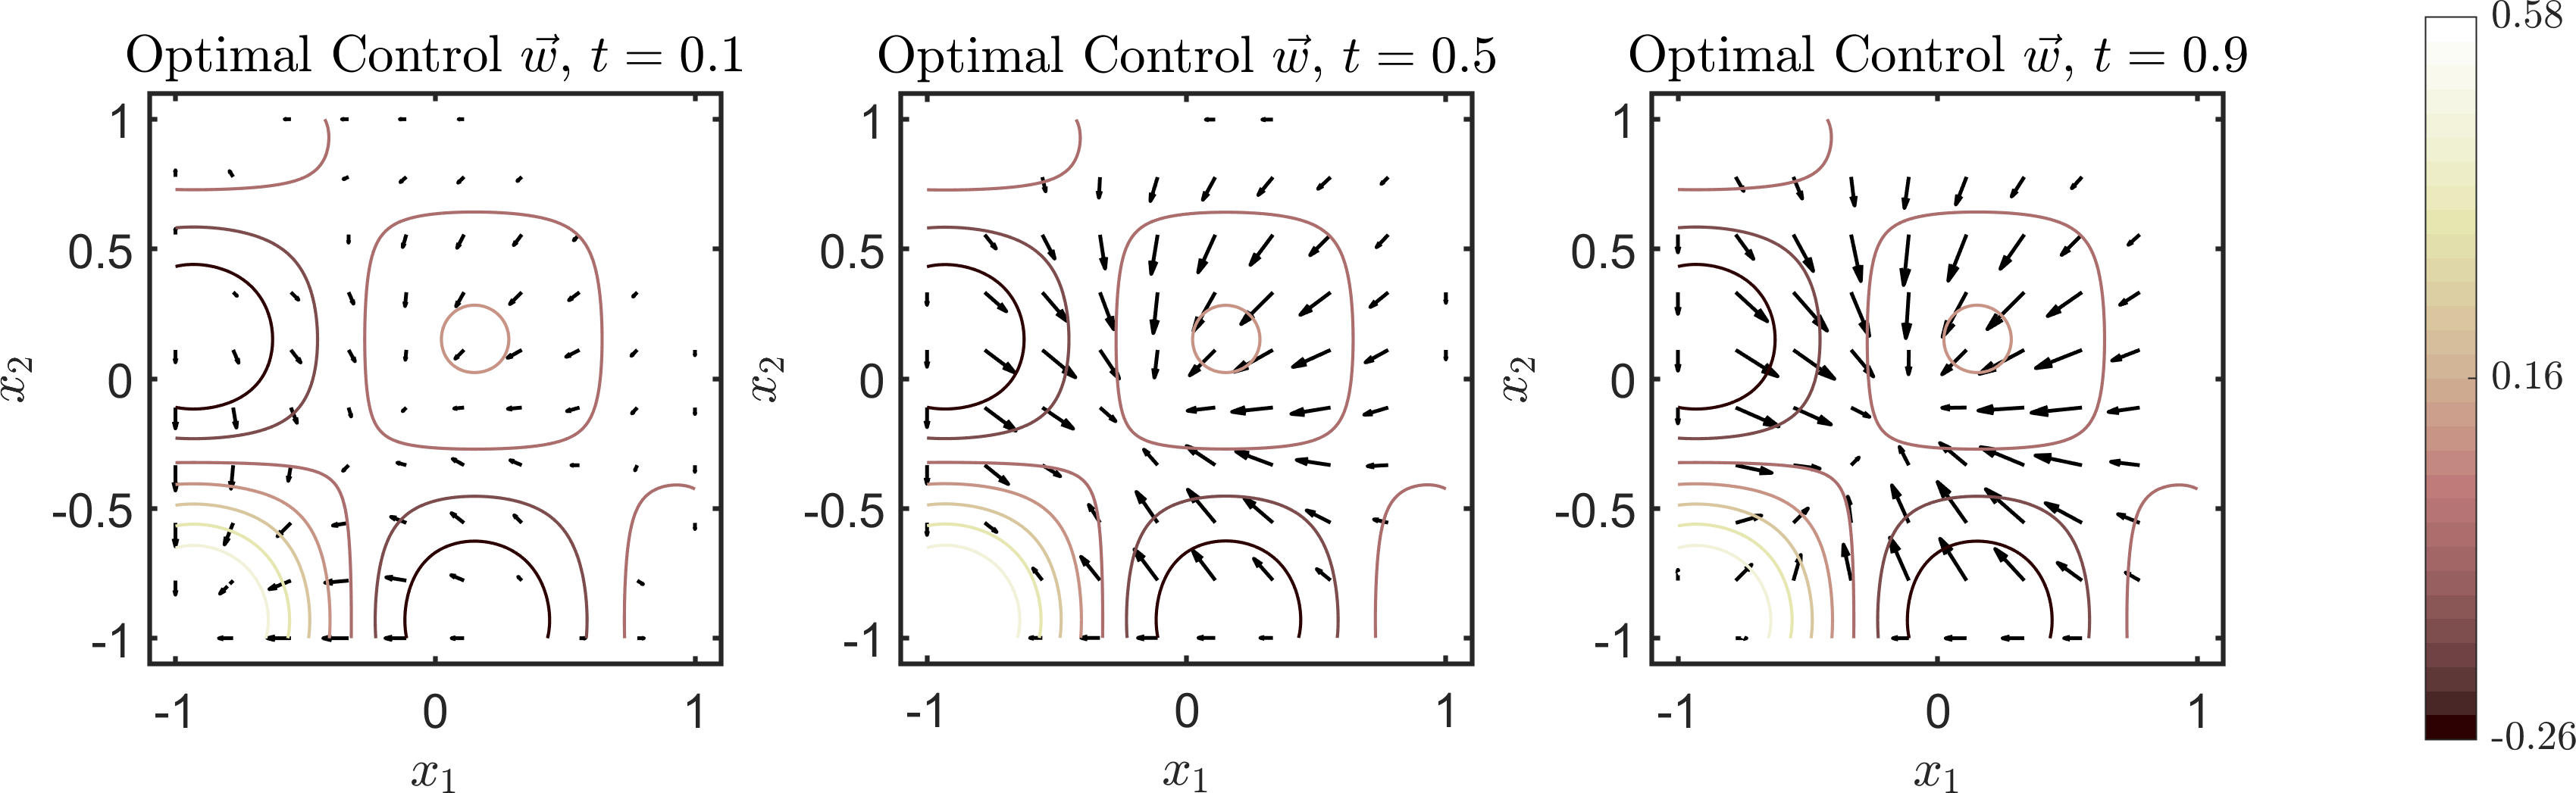
\includegraphics[scale=0.1]{FCNkn1c.png}
	\caption{Neumann Flow Control: Optimal control for $\kappa = -1$ and $\beta = 10^{-3}$ and contour plot of the external potential \emph{$V_{\text{ext}}$} as before.} 
	\label{F3bc}
\end{figure}
\begin{figure}[h]
	\centering
	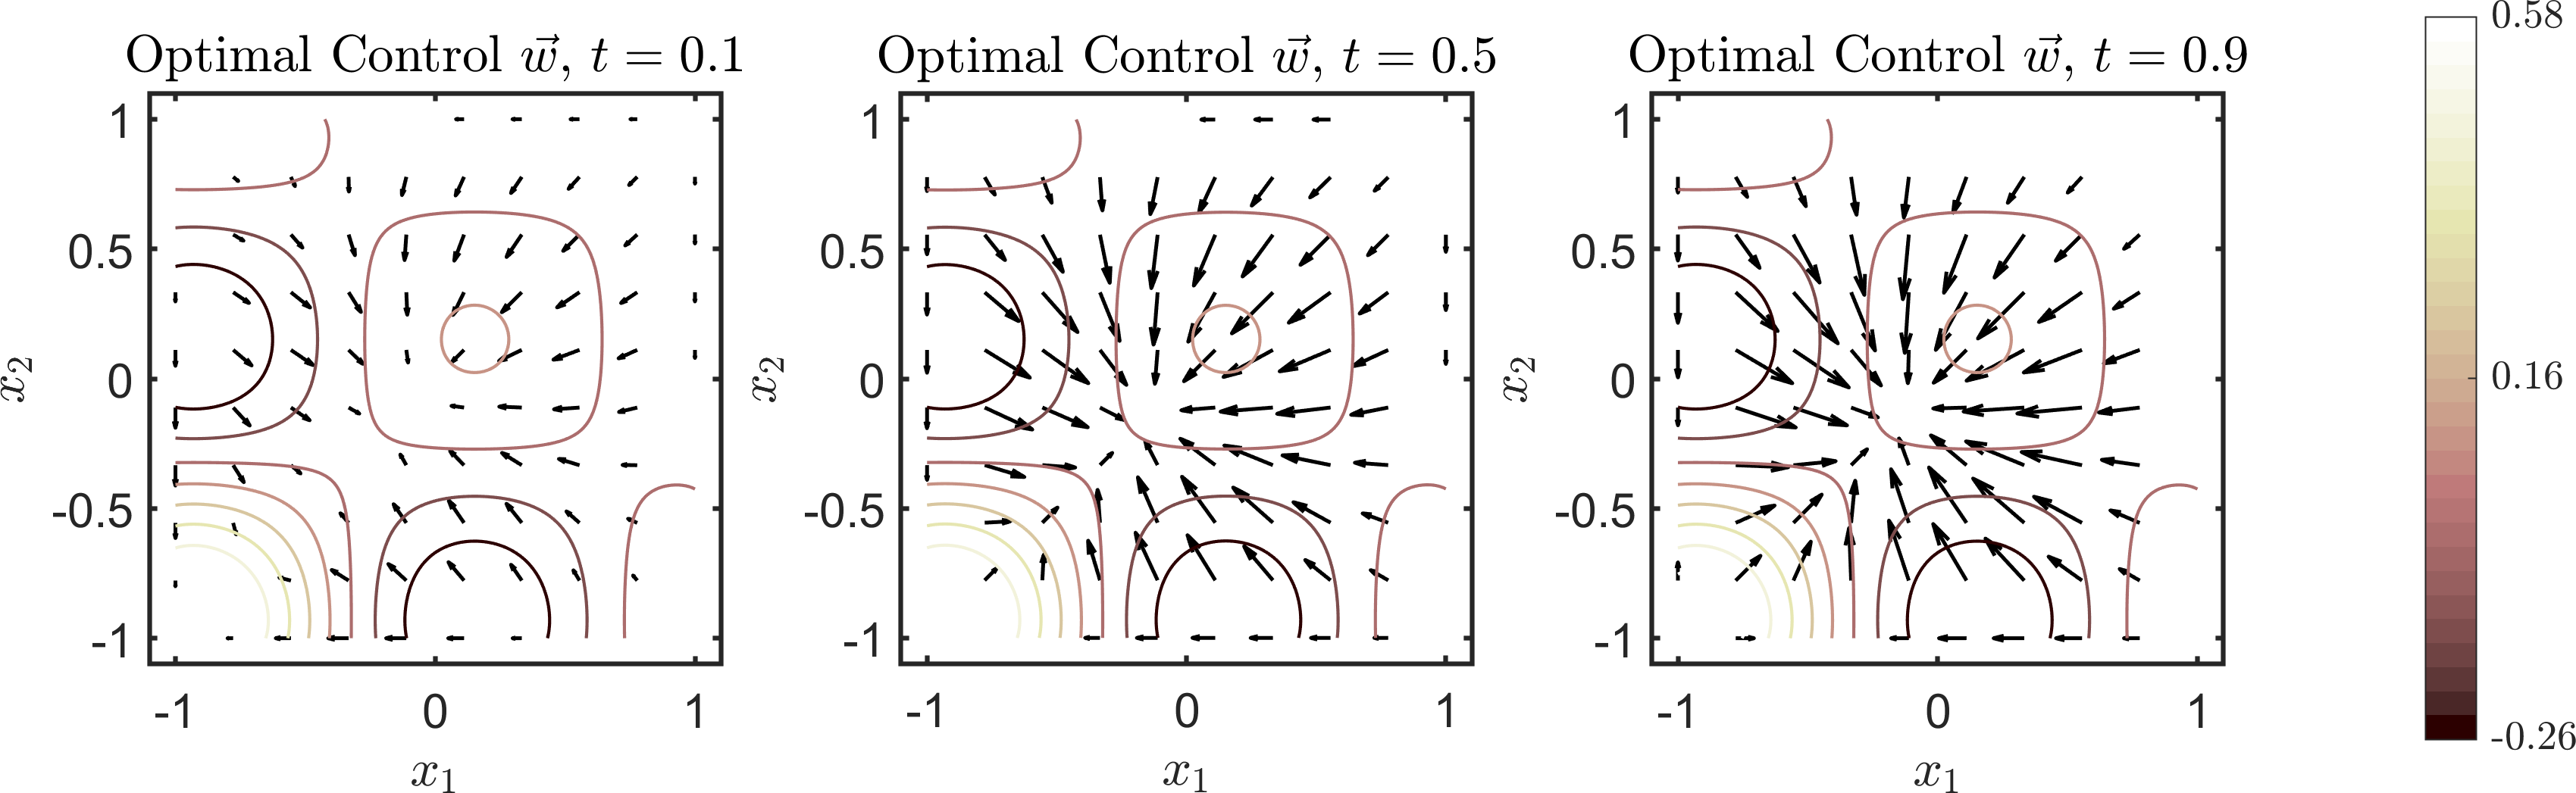
\includegraphics[scale=0.1]{FCNk1c.png}
	\caption{Neumann Flow Control: Optimal control for $\kappa = 1$ and $\beta = 10^{-3}$ and contour plot of the external potential \emph{$V_{\text{ext}}$} as before.} 
	\label{F3cc}
\end{figure}

\subsubsection{Non-linear (flow) control problem with Dirichlet boundary conditions}
The final 2D example is a flow control problem of type \eqref{AdvDiff}, with Dirichlet boundary conditions \eqref{Dirichlet}.
\begin{align*}
	\rho_0 &= \left(\frac{\pi}{4}\right)^2\cos\left(\frac{\pi x_1}{2}\right)\cos\left(\frac{\pi x_2}{2}\right) + \left(\frac{\pi}{4}\right)^2, \quad 
	V_{ext} = 2\sin\left(\frac{\pi x_1}{2}\right) \sin\left(\frac{\pi x_2}{3} - \frac{\pi}{2}\right),\\
	\hr &= (1 - t)\left(\left(\frac{\pi}{4}\right)^2\cos\left(\frac{\pi x_1}{2}\right)\cos\left(\frac{\pi x_2}{2}\right) + \left(\frac{\pi}{4}\right)^2\right) + t\left(\left(\frac{\pi}{4}\right)^2\cos\left(\frac{\pi x_1}{2}\right)\cos\left(\frac{3\pi x_2}{2}\right) + \left(\frac{\pi}{4}\right)^2\right).
\end{align*}
In this example the desired state prescribes the particles to move from one uniform bump in the middle of the domain, to accumulate in a steeper, elongated shape across the $x_1$-axis. In this example, the effect of the different interaction strengths and the external potential is clearly demonstrated, see Figure \ref{F5a}. The external potential is steep on the left side of the domain, so that most control effort is concentrated on the right side of the domain. However, for attractive particles, there also has to be more control applied in the right side of the domain, since the attractive particles work opposed to the action of spreading out along the $x_1$-axis, and the initial clump in the middle of the domain is a more natural state for this configuration, see Figure \ref{F5b}. Opposed to that is the effect that repulsive particles have on the control. In this case, most of the work of the control is done to push the particles together, see Figure \ref{F5c}. The controls can be seen in Figures \ref{F5ac}, \ref{F5bc} and \ref{F5cc}.
The results can be seen in Table \ref{TabFCD}.


\begin{table}
\centering
\begin{tabular}{ | c | c || c | c | c | c | c ||}
\hline
\multicolumn{2}{|c||}{}& $\beta = 10^{-5}$ & $\beta = 10^{-3}$ & $\beta = 10^{-1}$ & $\beta = 10^{1}$ & $\beta = 10^{3}$  \\
\hline
\hline
\multirow{2}{*}{$\kappa= \numprint{0}$}  & $\mathcal{J}_{uc}$ & $\numprint{0.1585}$ & $\numprint{0.1585}$ & $\numprint{0.1585}$ & $\numprint{0.1585}$ & $\numprint{0.1585}$\\
 & $\mathcal{J}_c$ & $\numprint{0.0004}$ & $\numprint{0.0077}$ & $\numprint{0.1302}$ & $\numprint{0.1582}$ & $\numprint{0.1585}$\\
\hline
\multirow{2}{*}{$\kappa= \numprint{1}$}  & $\mathcal{J}_{uc}$ & $\numprint{0.2124}$ & $\numprint{0.2124}$ & $\numprint{0.2124}$ & $\numprint{0.2124}$ & $\numprint{0.2124}$\\
 & $\mathcal{J}_c$ & $\numprint{0.0004}$ & $\numprint{0.0103}$ & $\numprint{0.1852}$ & $\numprint{0.2121}$ & $\numprint{0.2124}$\\
\hline
\multirow{2}{*}{$\kappa= \numprint{-1}$}  & $\mathcal{J}_{uc}$ & $\numprint{0.4031}$ & $\numprint{0.4031}$ & $\numprint{0.4031}$ & $\numprint{0.4031}$ & $\numprint{0.4031}$\\
 & $\mathcal{J}_c$ & $\numprint{0.0005}$ & $\numprint{0.0086}$ & $\numprint{0.1739}$ & $\numprint{0.3867}$ & $\numprint{0.4029}$\\
\hline
\end{tabular}
\caption{Flow Control Dirichlet Problem: Cost when $w=0$ and optimal control cost for a range of $\kappa$, $\beta$. For $\beta = 10$, the cost functionals differ by $10^-4$ for $\kappa = 0$ and $\kappa = 1$ and by $10^-2$ for $\kappa = -1$. For $\beta = 10^3$, the cost functionals differ by $10^{-7}$ for $\kappa = 0$, by $10^{-6}$ for $\kappa = 1$, and by $10^{-4}$ for $\kappa = -1$.}
\label{TabFCD}
\end{table}

\begin{figure}[h]
	\centering
	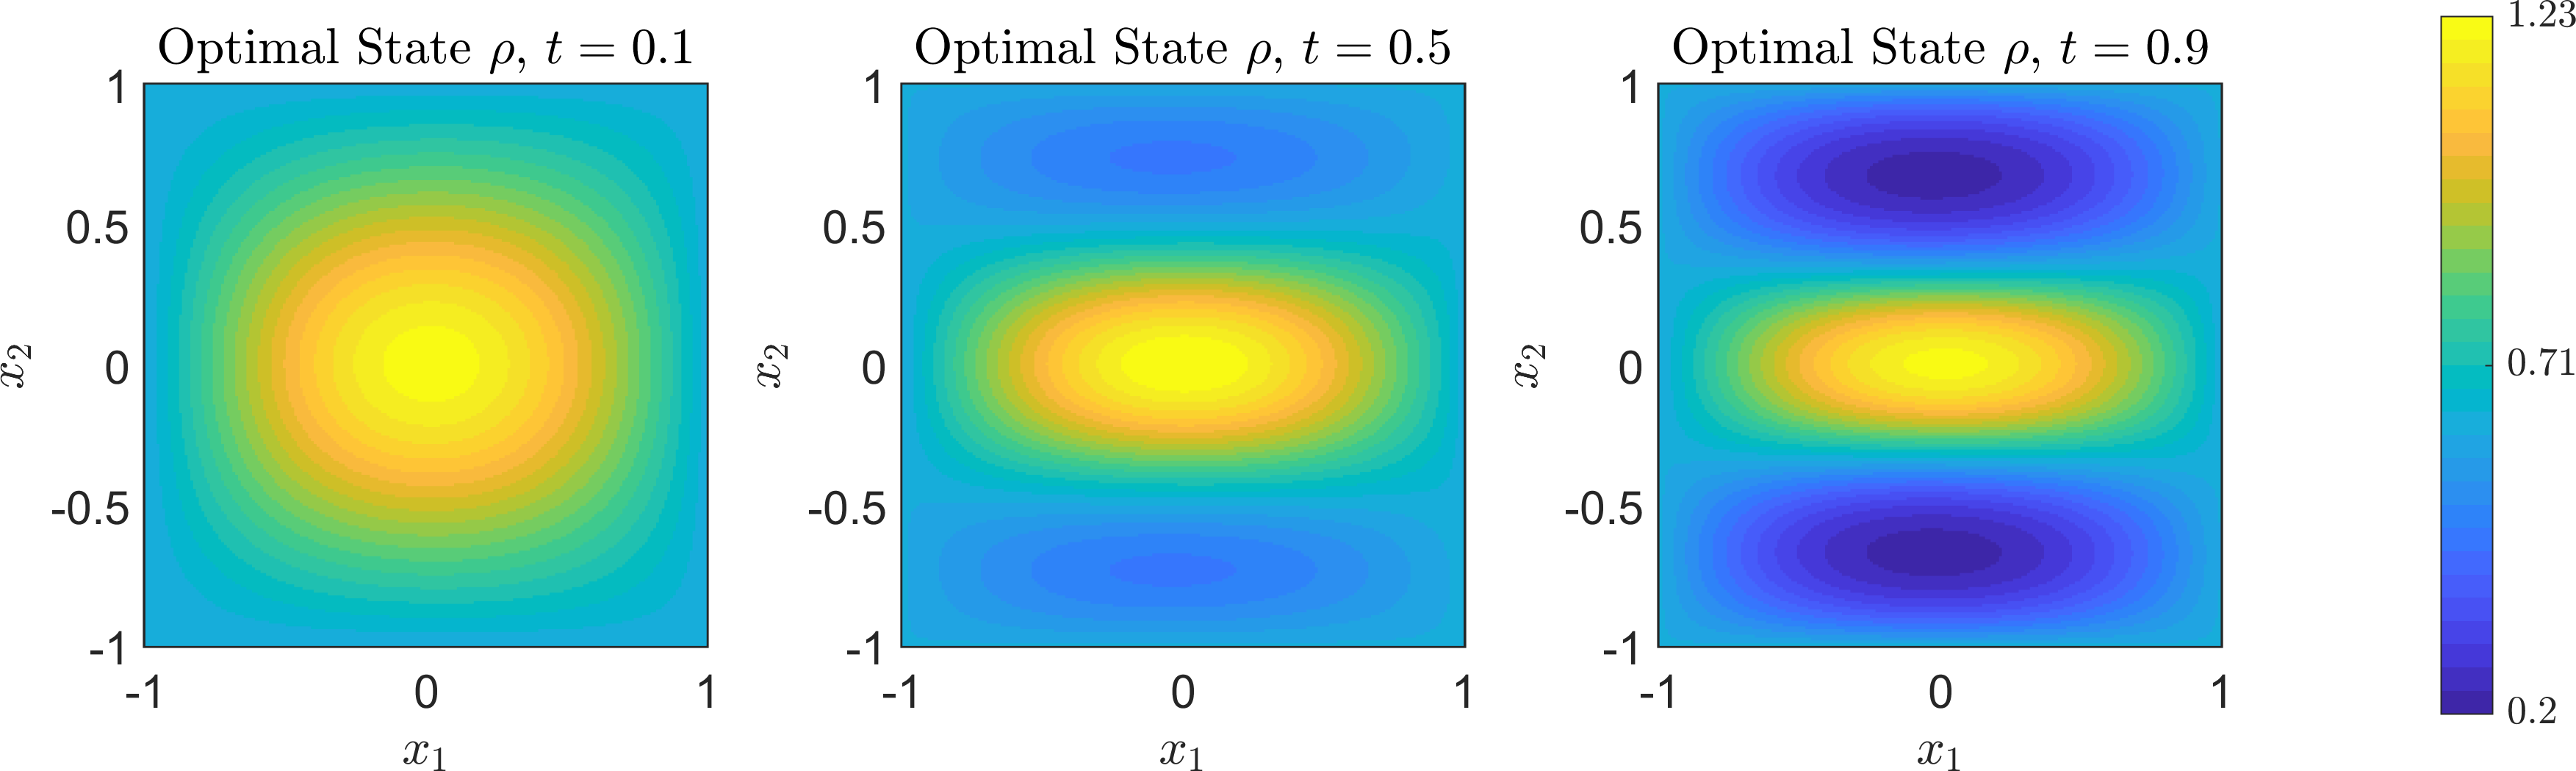
\includegraphics[scale=0.1]{FCDk0.png}
	\caption{Dirichlet Flow Control: Optimal $\rho$ for $\kappa = 0$ and $\beta = 10^{-3}$.} 
	\label{F5a}
\end{figure}
\begin{figure}[h]
	\centering
	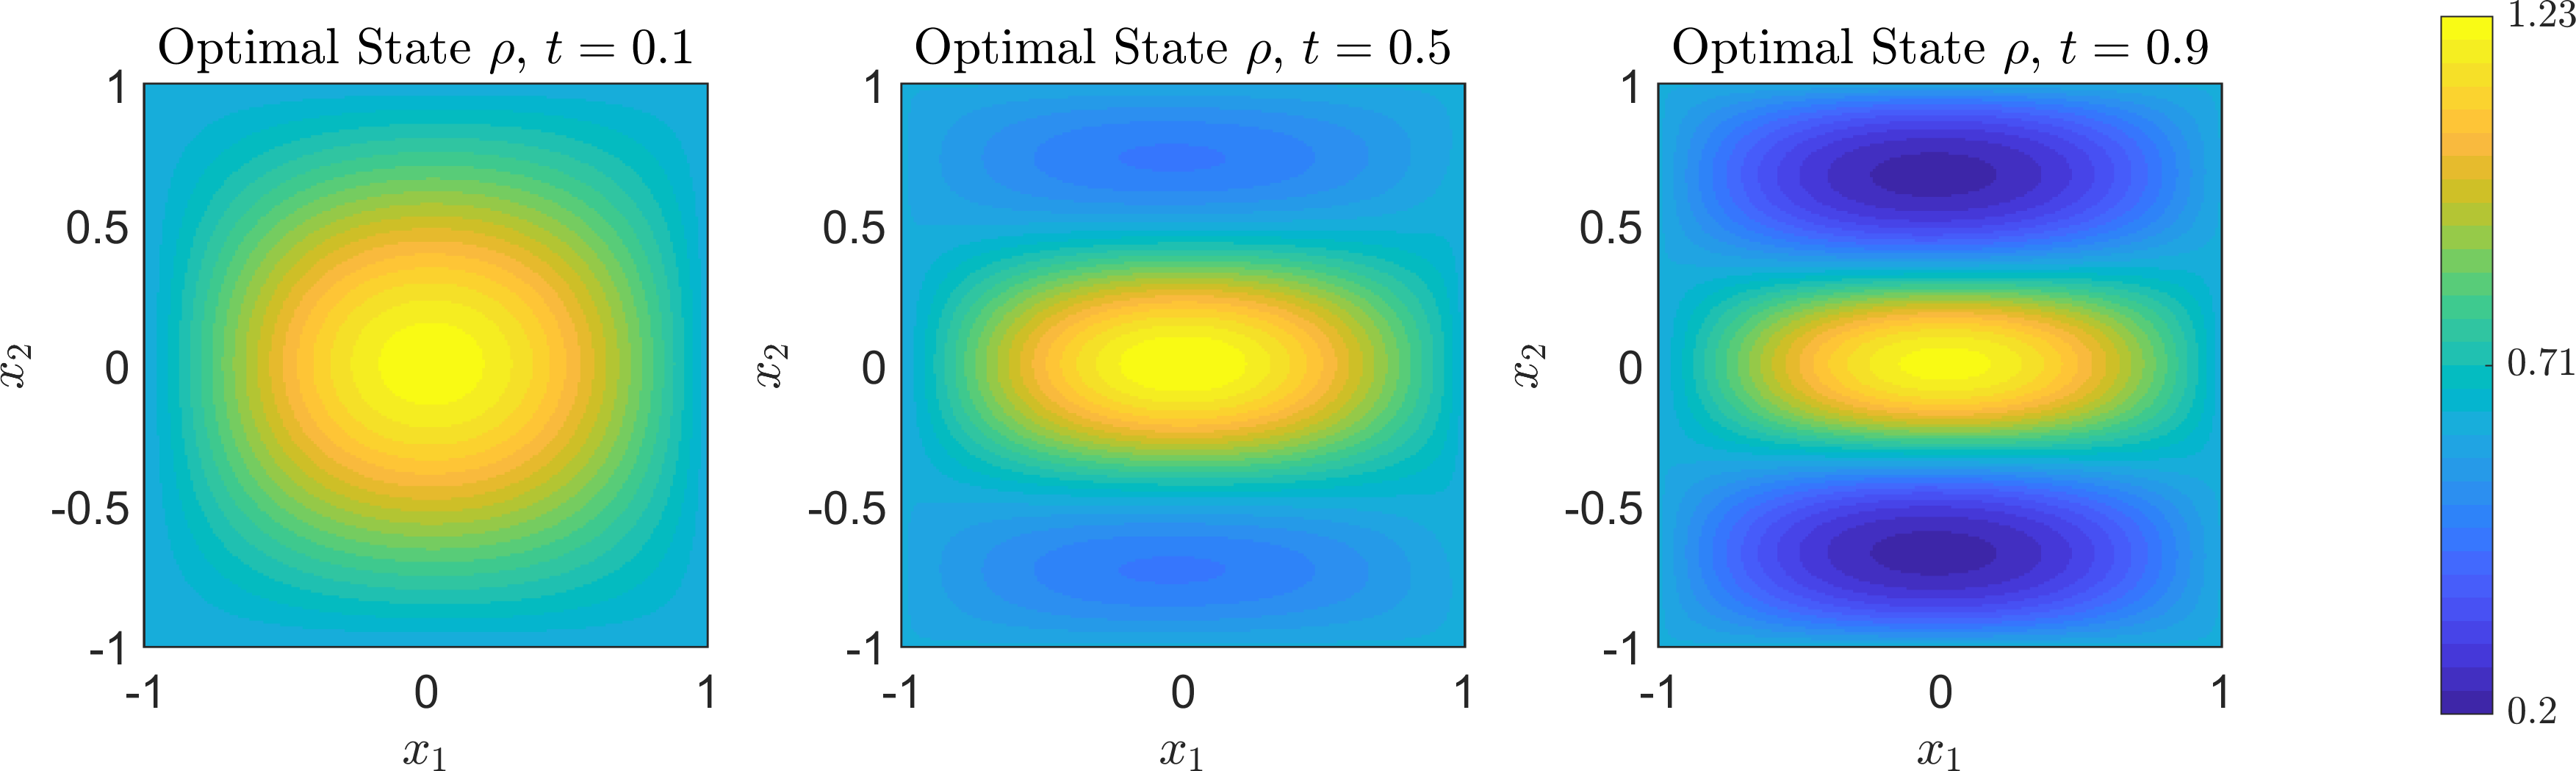
\includegraphics[scale=0.1]{FCDkn1.png}
	\caption{Dirichlet Flow Control: Optimal $\rho$ for $\kappa = -1$ and $\beta = 10^{-3}$.} 
	\label{F5b}
\end{figure}
\begin{figure}[h]
	\centering
	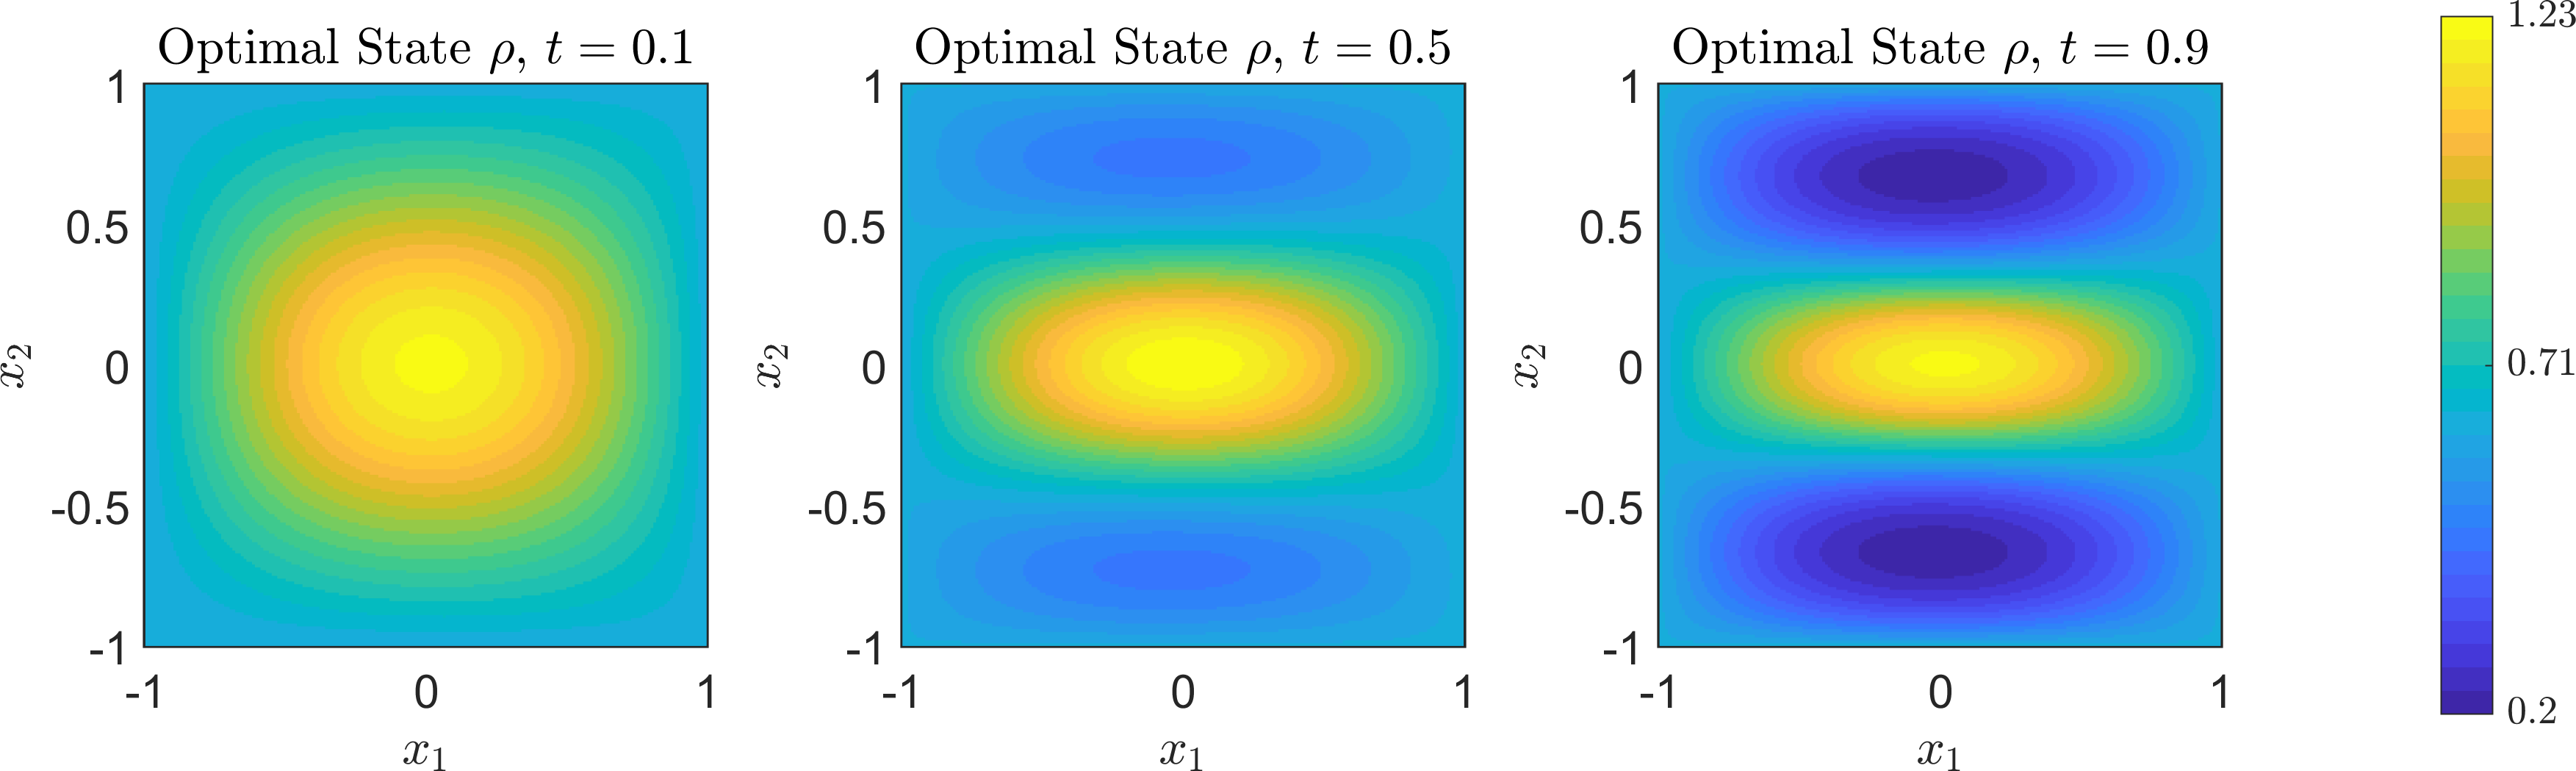
\includegraphics[scale=0.1]{FCDk1.png}
	\caption{Dirichlet Flow Control: Optimal $\rho$ for $\kappa = 1$ and $\beta = 10^{-3}$.} 
	\label{F5c}
\end{figure}



\begin{figure}[h]
	\centering
	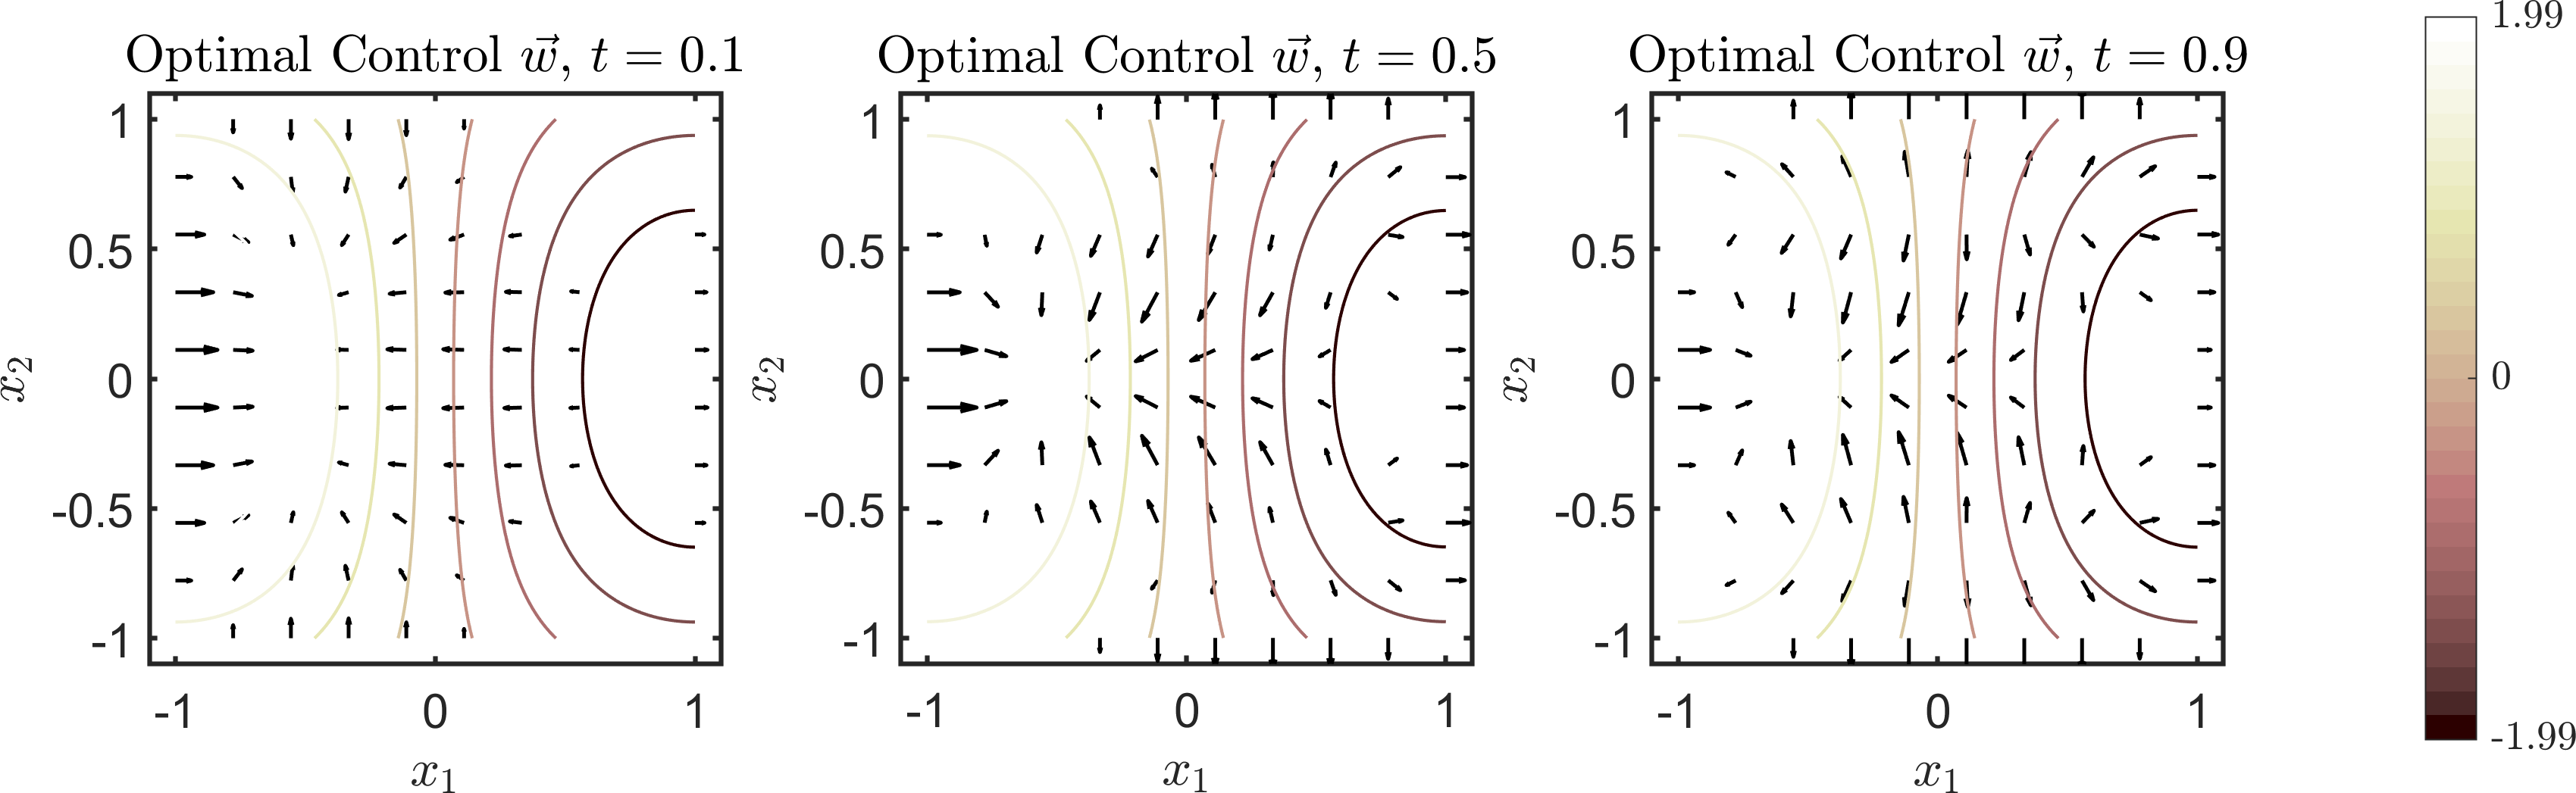
\includegraphics[scale=0.1]{FCDk0c.png}
	\caption{Dirichlet Flow Control: Optimal control for $\kappa = 0$ and $\beta = 10^{-3}$. A contour plot of the external potential \emph{$V_{\text{ext}}$} is superimposed on the control plots for reference, with a corresponding colorbar on the left-hand side.} 
	\label{F5ac}
\end{figure}
\begin{figure}[h]
	\centering
	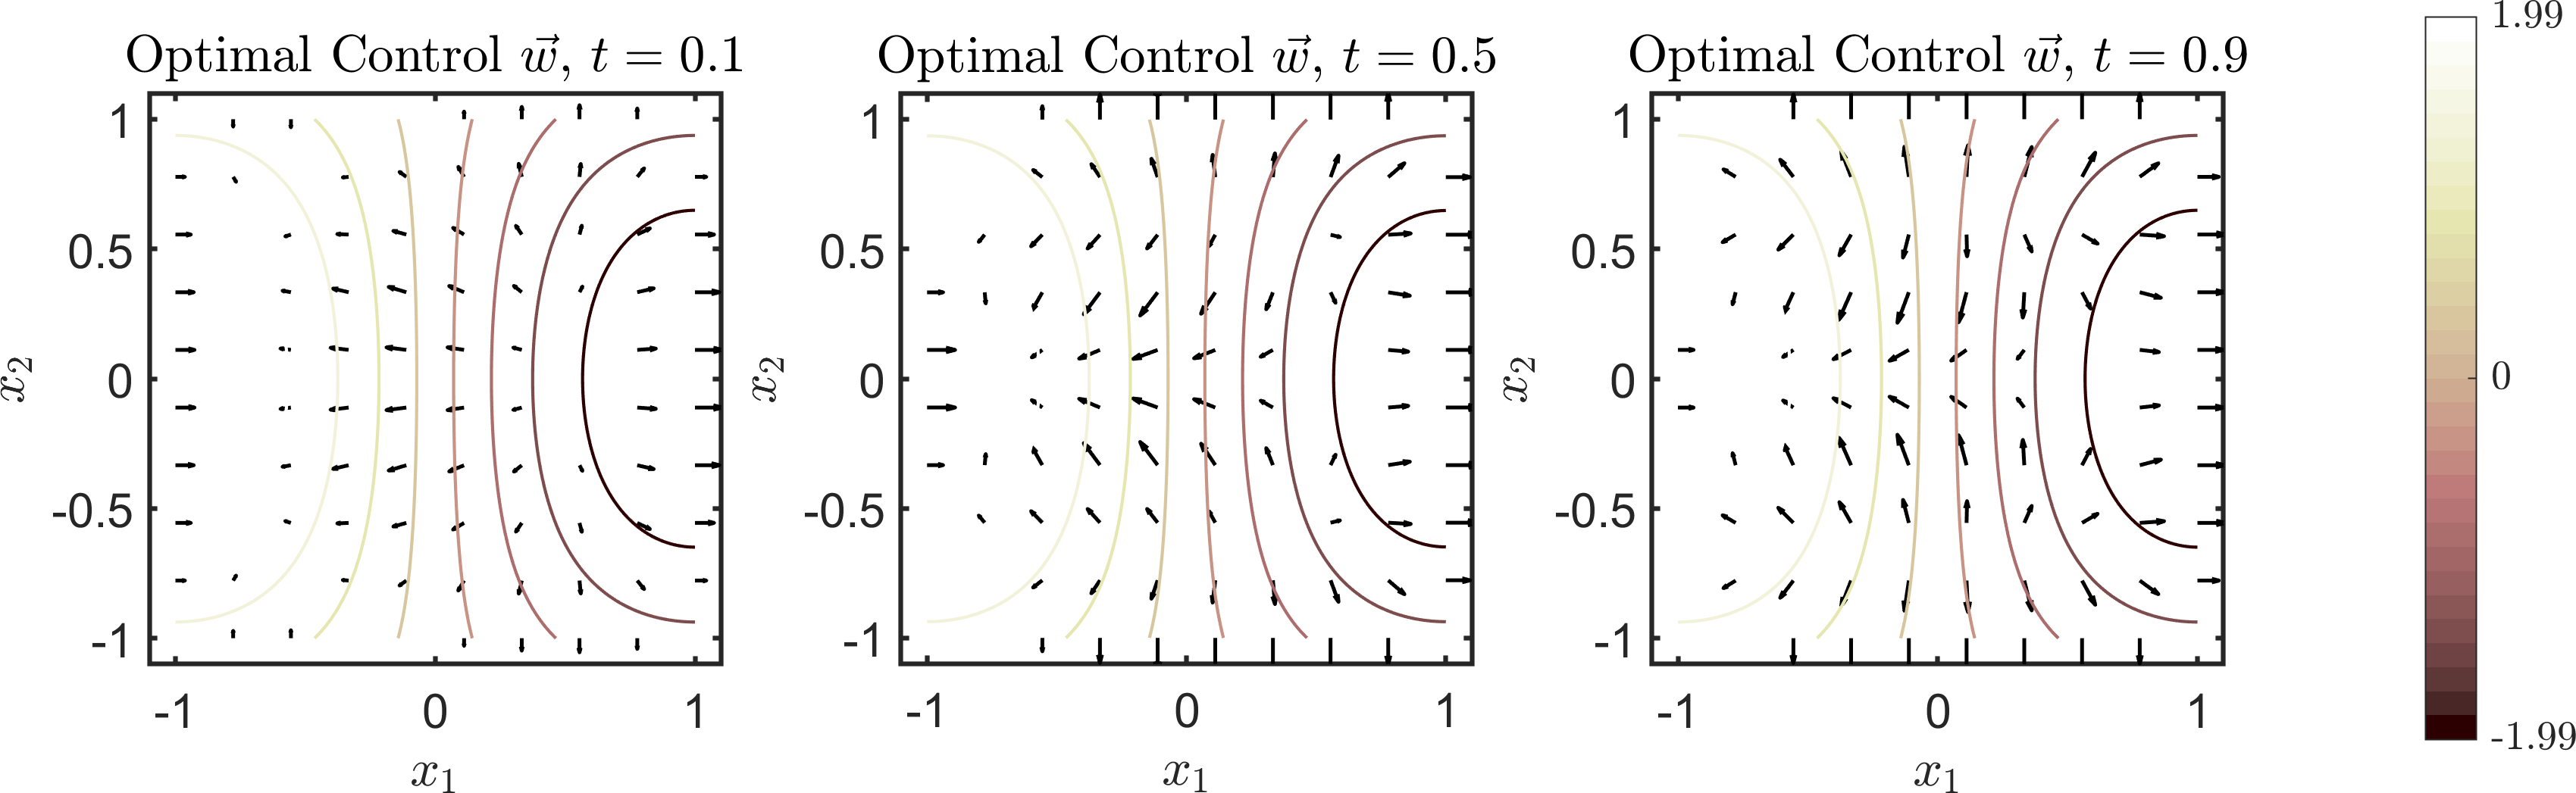
\includegraphics[scale=0.1]{FCDkn1c.png}
	\caption{Dirichlet Flow Control: Optimal control for $\kappa = -1$ and $\beta = 10^{-3}$ and contour plot of the external potential \emph{$V_{\text{ext}}$} as before.} 
	\label{F5bc}
\end{figure}
\begin{figure}[h]
	\centering
	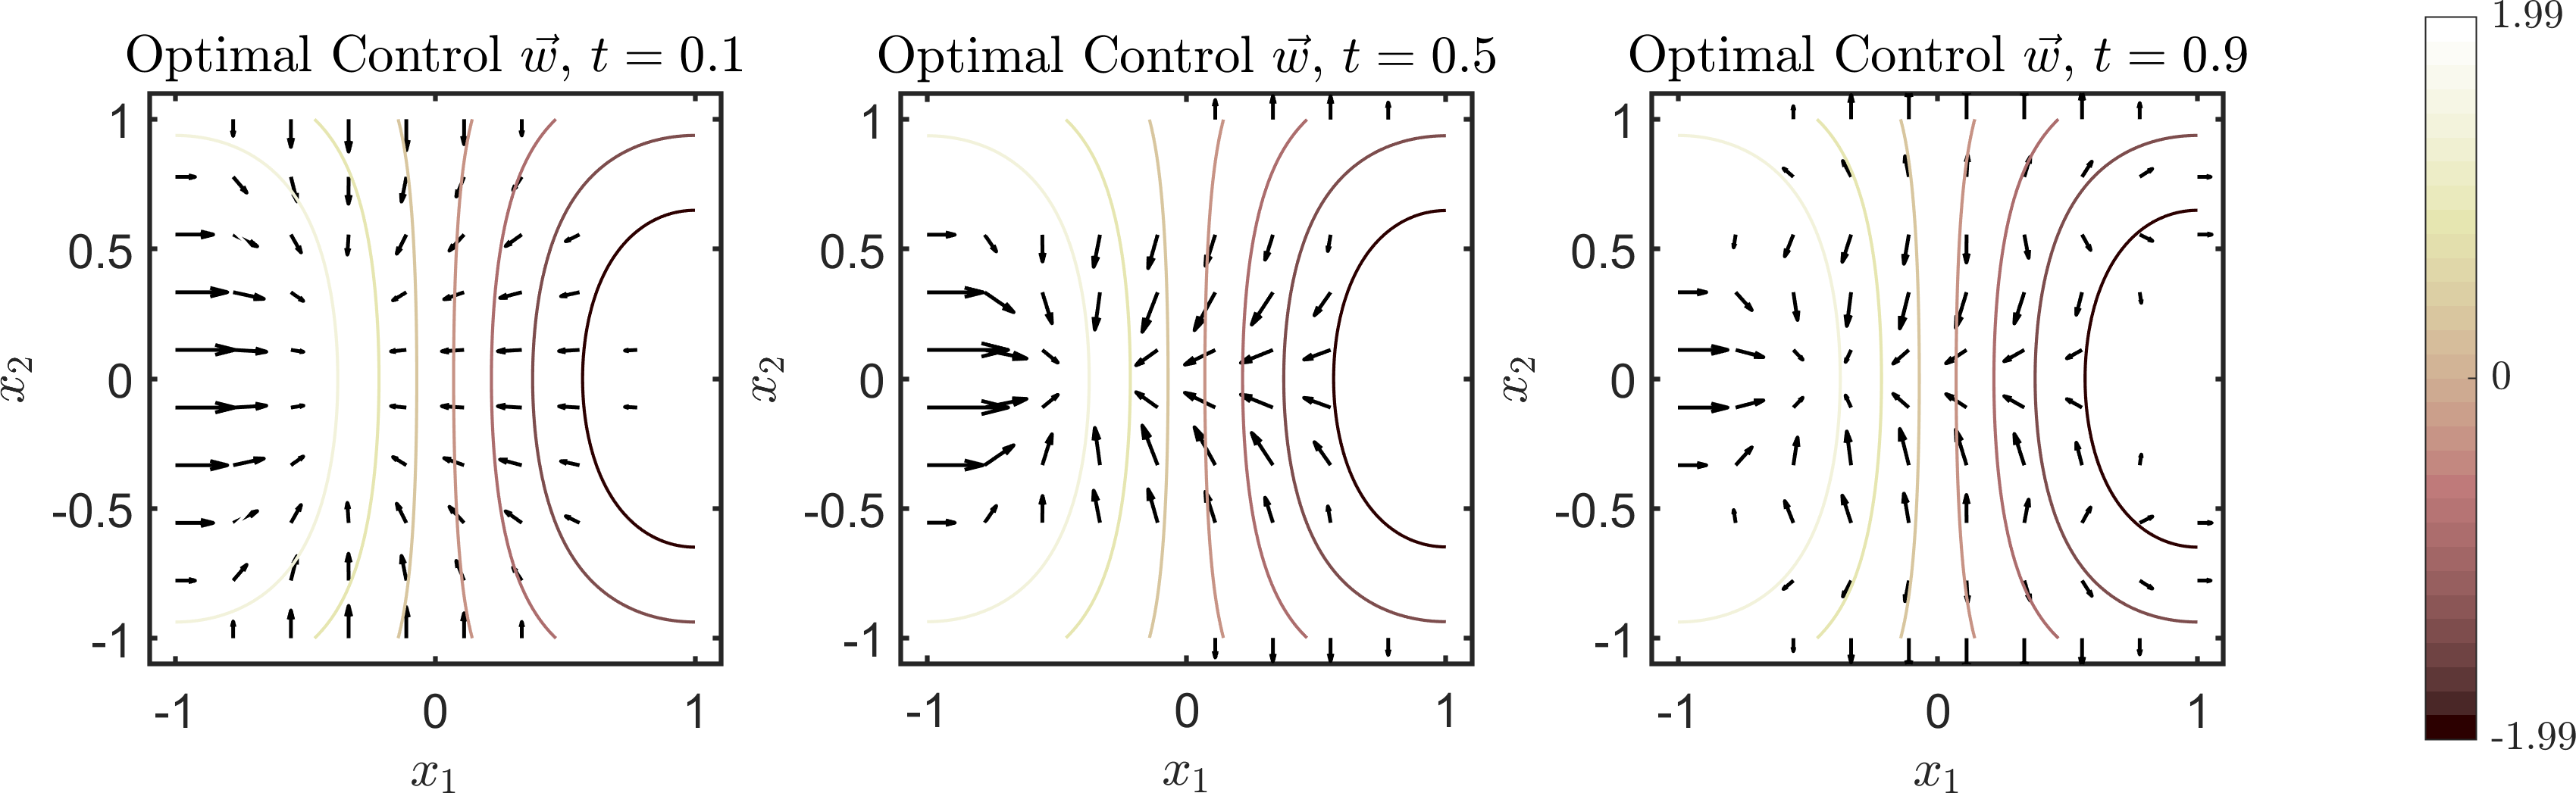
\includegraphics[scale=0.1]{FCDk1c.png}
	\caption{Dirichlet Flow Control: Optimal control for $\kappa = 1$ and $\beta = 10^{-3}$ and contour plot of the external potential \emph{$V_{\text{ext}}$} as before.} 
	\label{F5cc}
\end{figure}

\subsection{Three-dimensional Example}
We consider a three-dimensional example featuring the non-linear flow control problem \eqref{AdvDiff} with boundary conditions \eqref{NoFlux}, since this is the most challenging combination of control type and boundary conditions.
The chosen inputs for this example are:
\begin{align*}
	\rho_0 &= \frac{1}{8}, \quad \hr = \frac{1}{8}(1-t) + t\left(\frac{\pi}{4}\right)^3\cos\left(\frac{\pi x_1}{2}\right)\cos\left(\frac{\pi x_2}{2}\right)\cos\left(\frac{\pi x_3}{2}\right),\\
	V_{ext} &= \left(\left(x_1 + 0.3\right)^2 - 1\right)\left(\left(x_1 - 0.4\right)^2 - 0.5\right) \left(\left(x_2 + 0.3\right)^2 - 1\right)\left(\left(x_2 - 0.4\right)^2 - 0.5\right)\\
	&\ \quad\left(\left(x_3 + 0.3\right)^2 - 1\right)\left(\left(x_3 - 0.4\right)^2 - 0.5\right).
\end{align*}
The effect of the different interaction strengths is clearly displayed in Figures \ref{F2}, \ref{F3} and \ref{F4} and is particularly obvious in earlier times of the particle evolution.
The imposed external potential is shown in Figure \ref{F1}.
In Figures \ref{F5}, \ref{F6} and \ref{F7}, the controls for different interaction strengths are shown. It is evident, that attractive particles support the control to push the particles into a cluster in the middle of the domain, as prescribed by the desired state $\hr$, while more control is needed for a similar effect in the repulsive setup.
This example is only run for $\beta = 10^{-3}$, due to a running time of approximately $35$ hours per problem. We get for $\kappa = 0$, $\mathcal J_c = 0.0078$. This can be compared to $\mathcal J_{uc} = 0.0195$ from the computed forward problem with $\w = \vec 0$. For $\kappa = 1$, we get that $\mathcal J_c = 0.0102$ as opposed to $\mathcal J_{uc} = 0.0232$ in the uncontrolled case and for $\kappa = -1$ we have $\mathcal J_c = 0.0059$, which is compared to the uncontrolled value $\mathcal J_{uc} = 0.0477$.


	\begin{figure}[h]
		\centering
		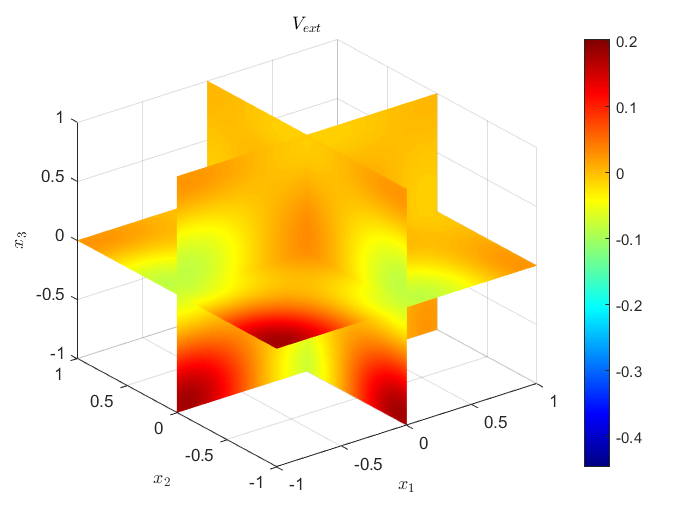
\includegraphics[scale=0.7]{Vext3D.png}
		\caption{External Potential $V_{ext}$} 
		\label{F1}
	\end{figure}

	

\begin{figure}[h]
	\centering
	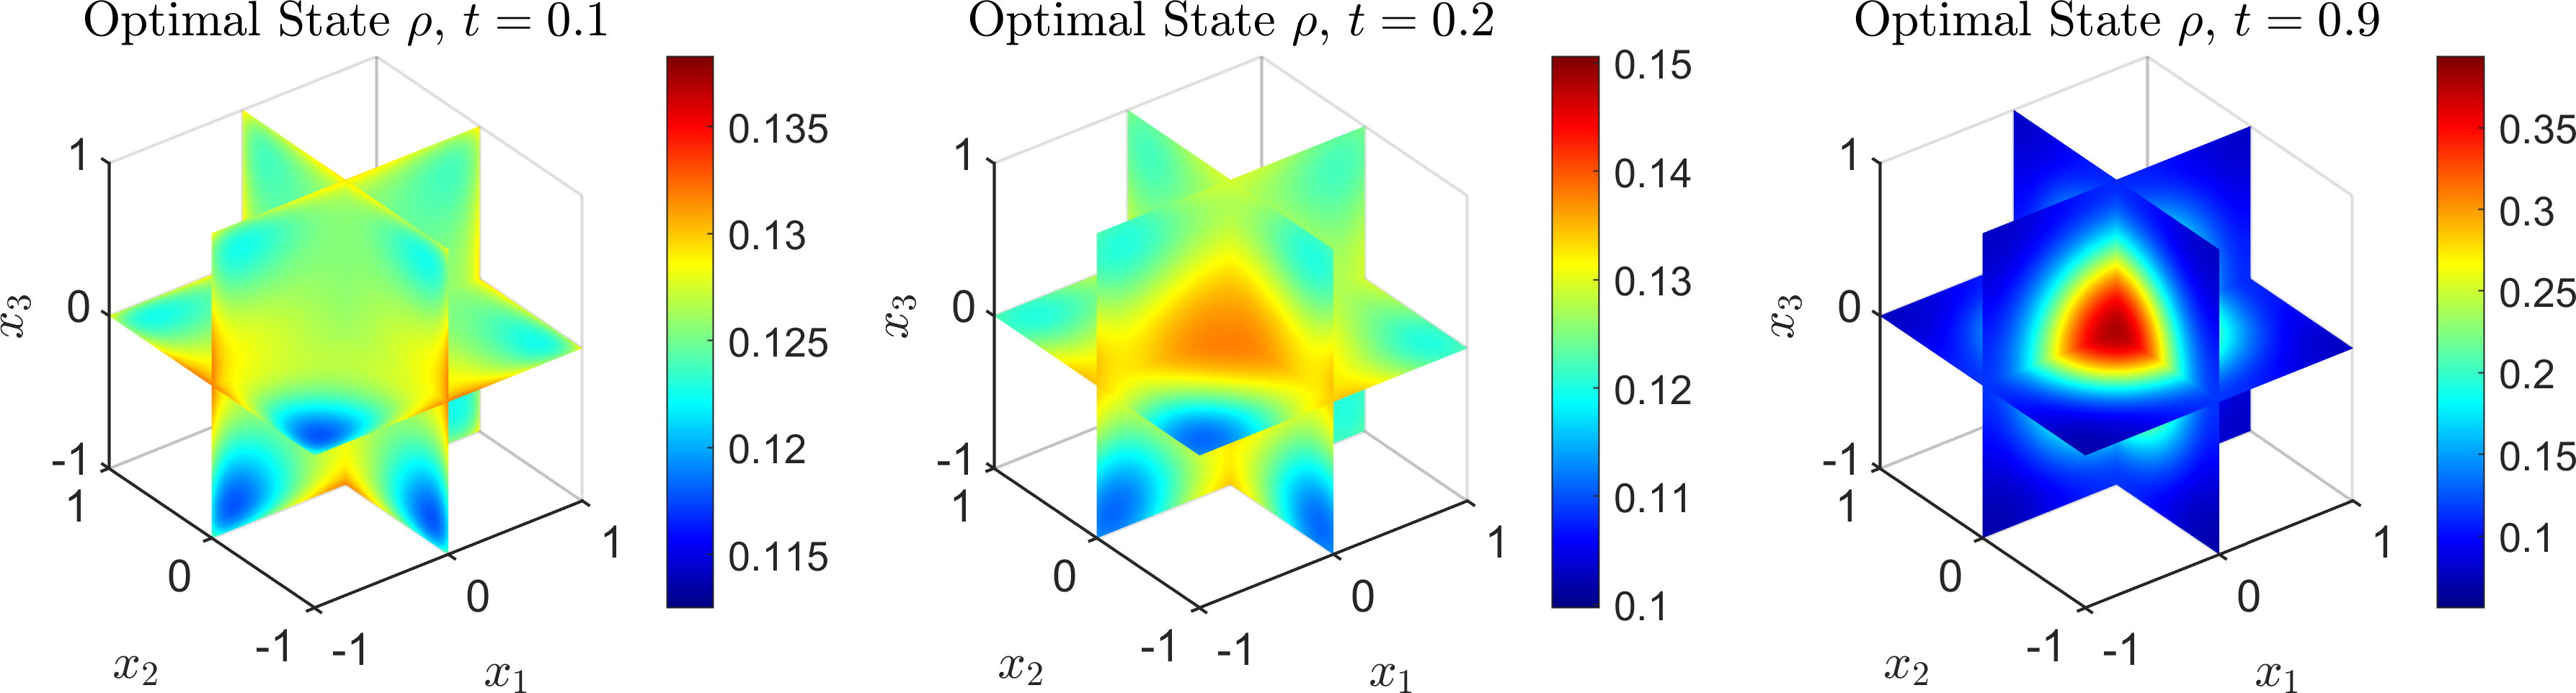
\includegraphics[scale=0.1]{rhok1.png}
	\caption{Optimal state $\rho$ for $\kappa = 1$.} 
	\label{F2}
\end{figure}
\begin{figure}[h]
	\centering
	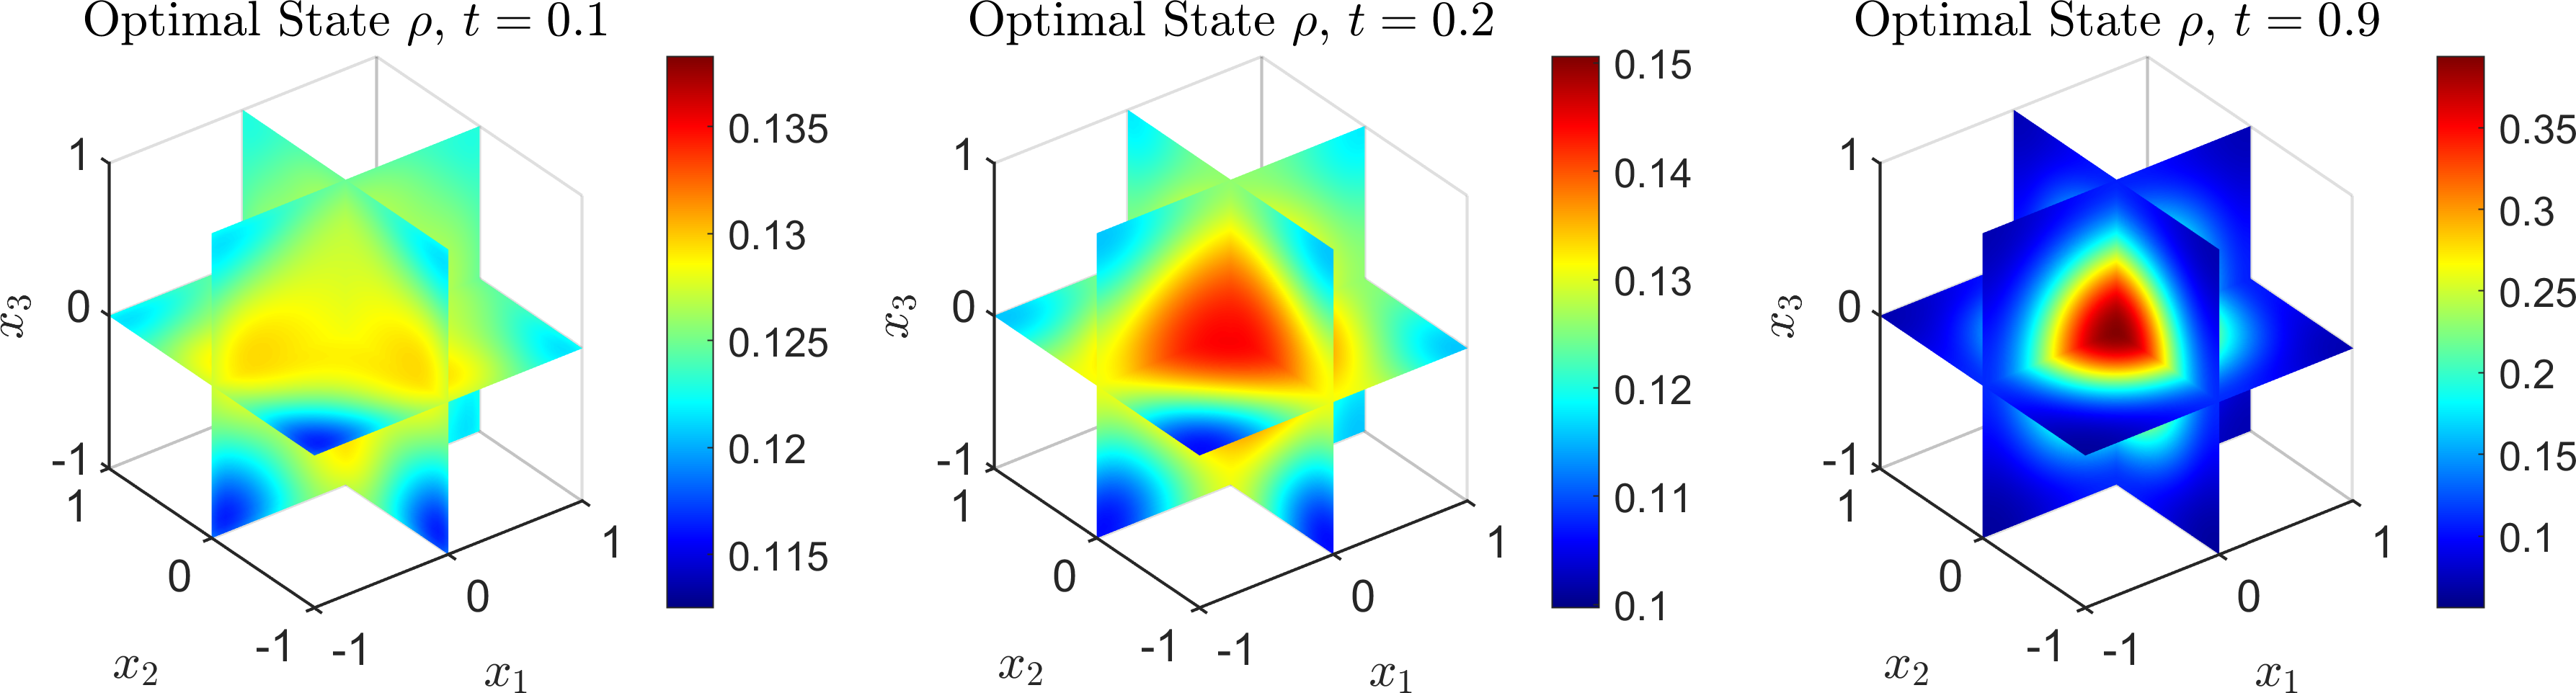
\includegraphics[scale=0.1]{rhok0.png}
	\caption{Optimal state $\rho$ for $\kappa = 0$.} 
	\label{F3}
\end{figure}
\begin{figure}[h]
	\centering
	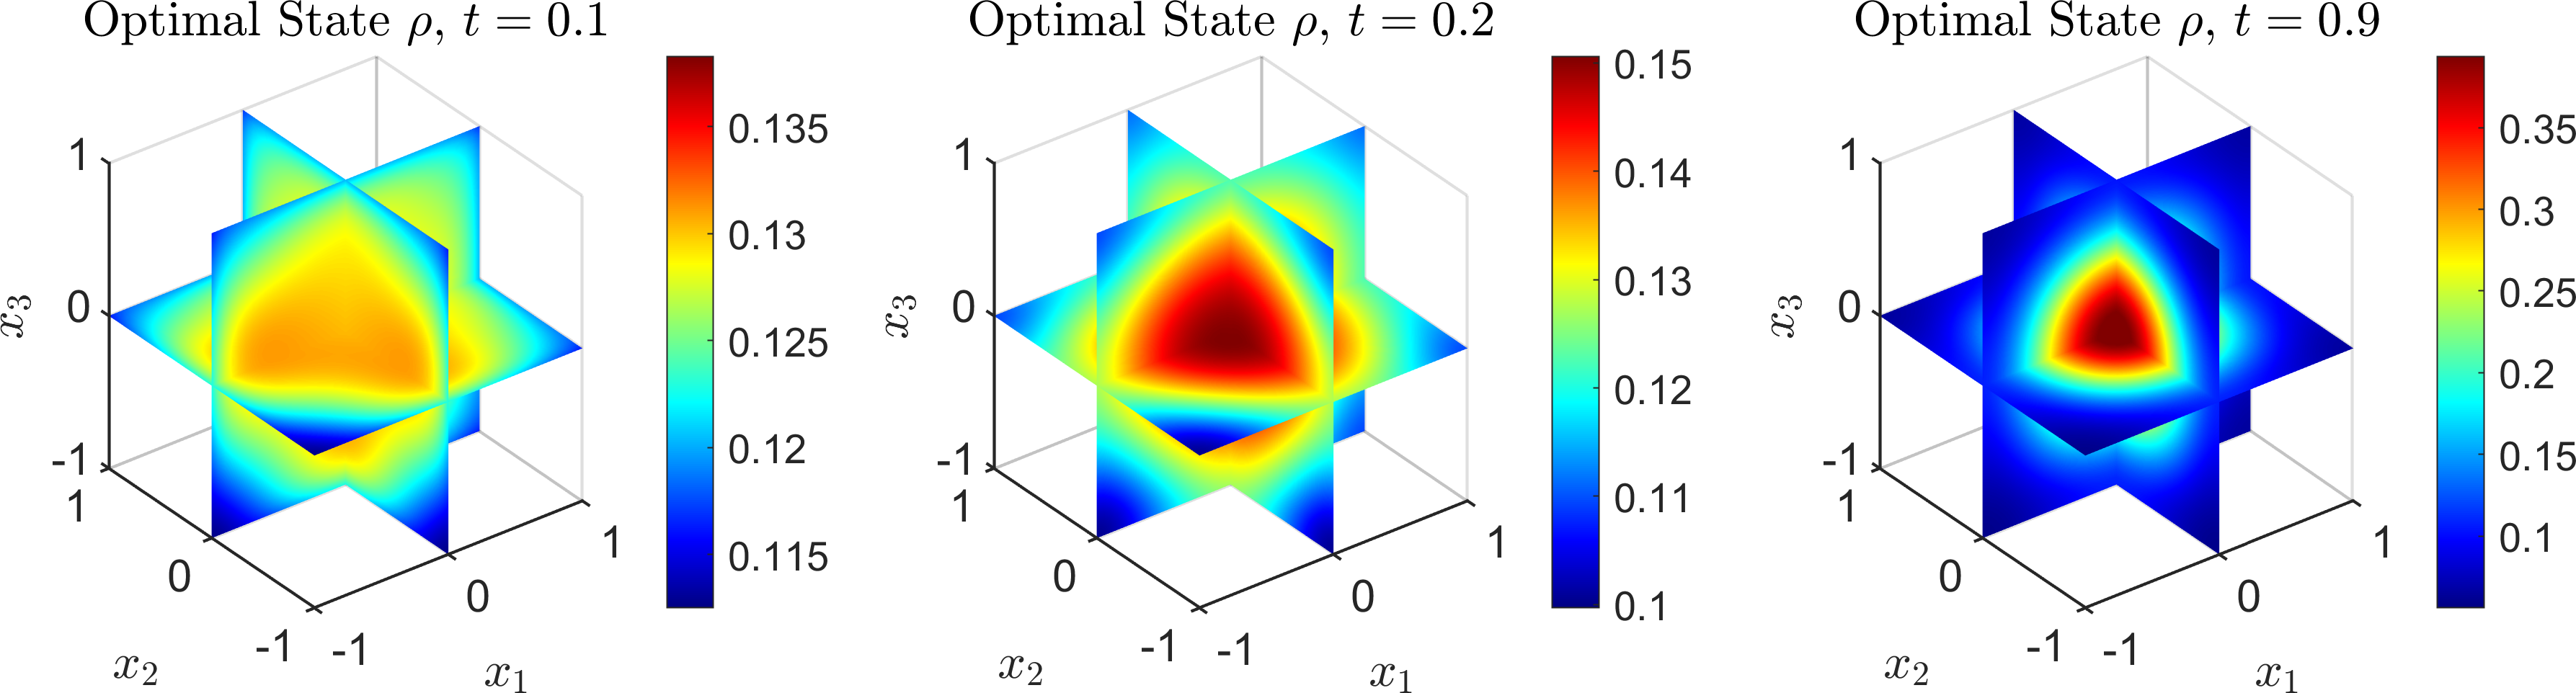
\includegraphics[scale=0.1]{rhokn1.png}
	\caption{Optimal state $\rho$ for $\kappa = -1$.} 
	\label{F4}
\end{figure}
%	
\begin{figure}[h]
	\centering
	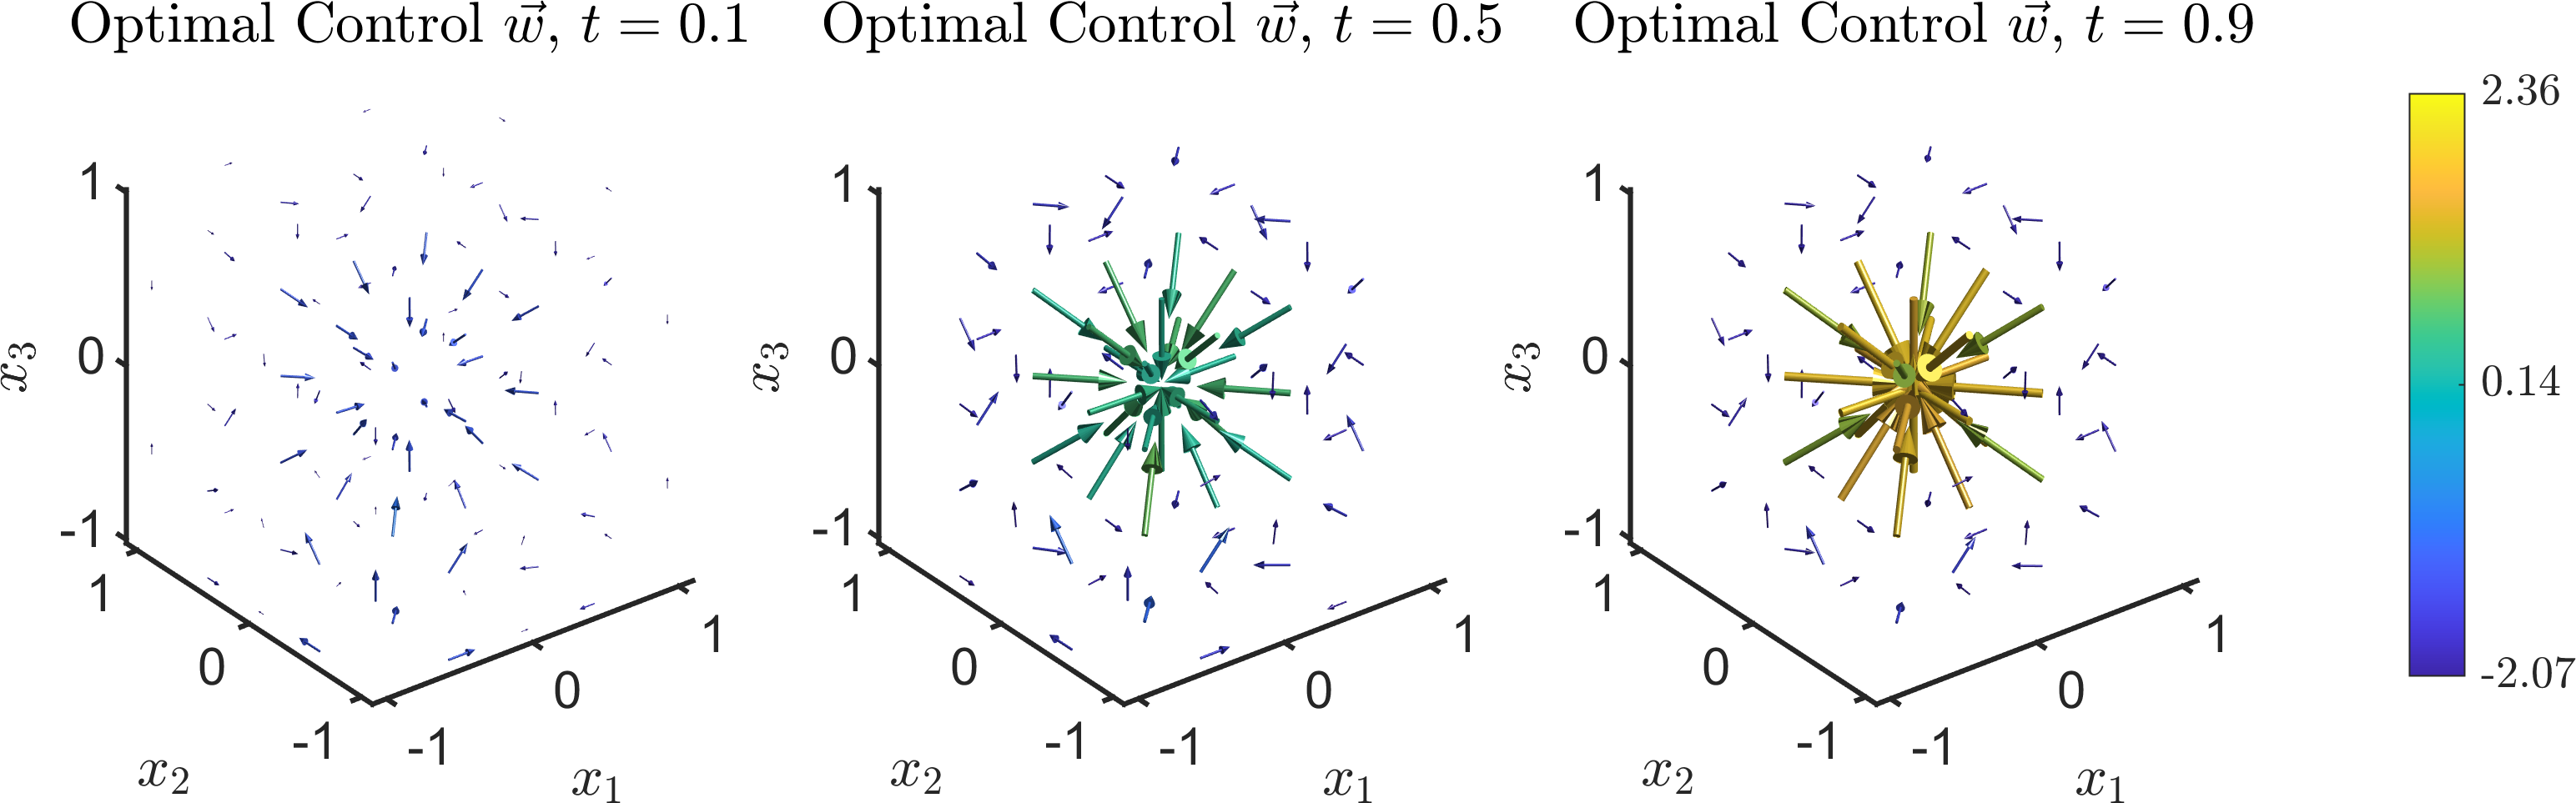
\includegraphics[scale=0.1]{Controlk1.png}
	\caption{Optimal control $\w$ for $\kappa = 1$.} 
	\label{F5}
\end{figure}
\begin{figure}[h]
	\centering
	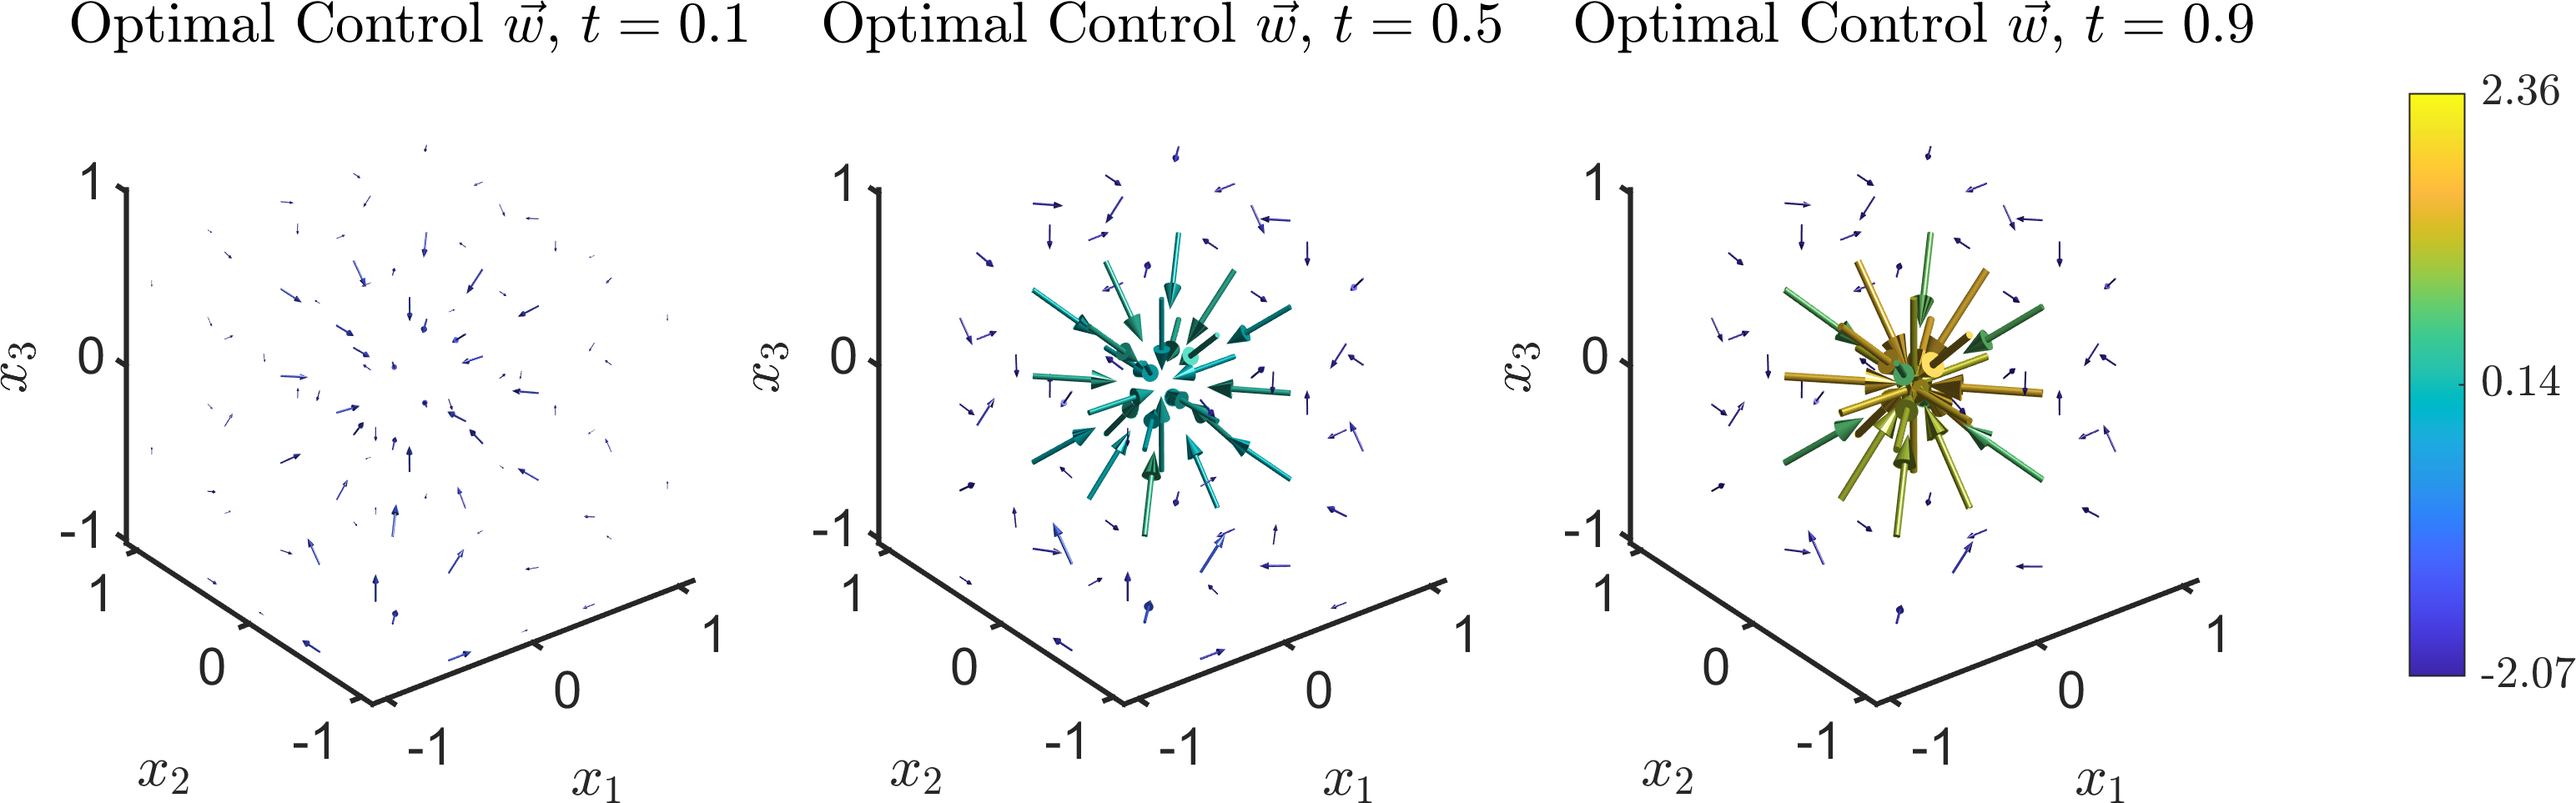
\includegraphics[scale=0.1]{Controlk0.png}
	\caption{Optimal control $\w$ for $\kappa = 0$.} 
	\label{F6}
\end{figure}
\begin{figure}[h]
	\centering
	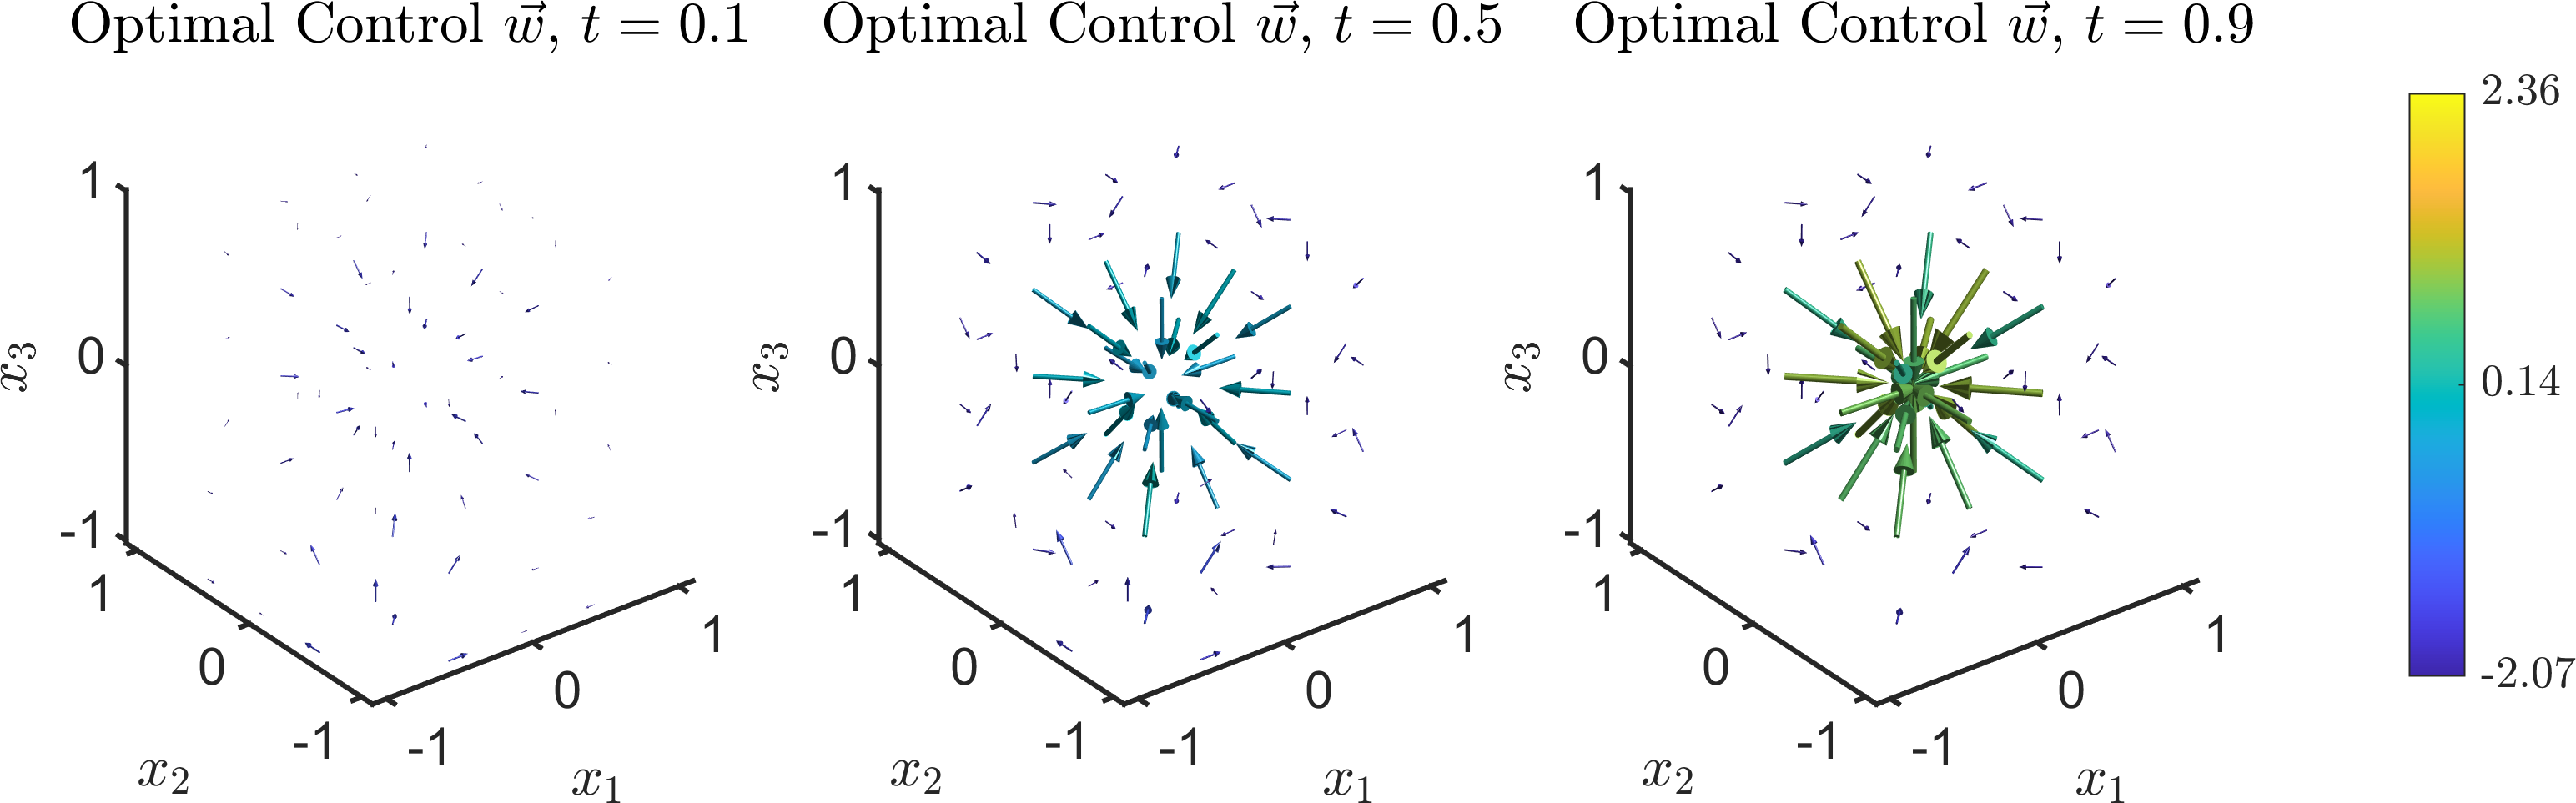
\includegraphics[scale=0.1]{Controlkn1.png}
	\caption{Optimal control $\w$ for $\kappa = -1$.} 
	\label{F7}
\end{figure}

Figures \ref{Con1}, \ref{Con2}, \ref{Con3} and \ref{Con4} show the convergence of the Newton-Krylov method for different $\beta$ for each 2D problem considered above.

\begin{figure}[h]
	\centering
	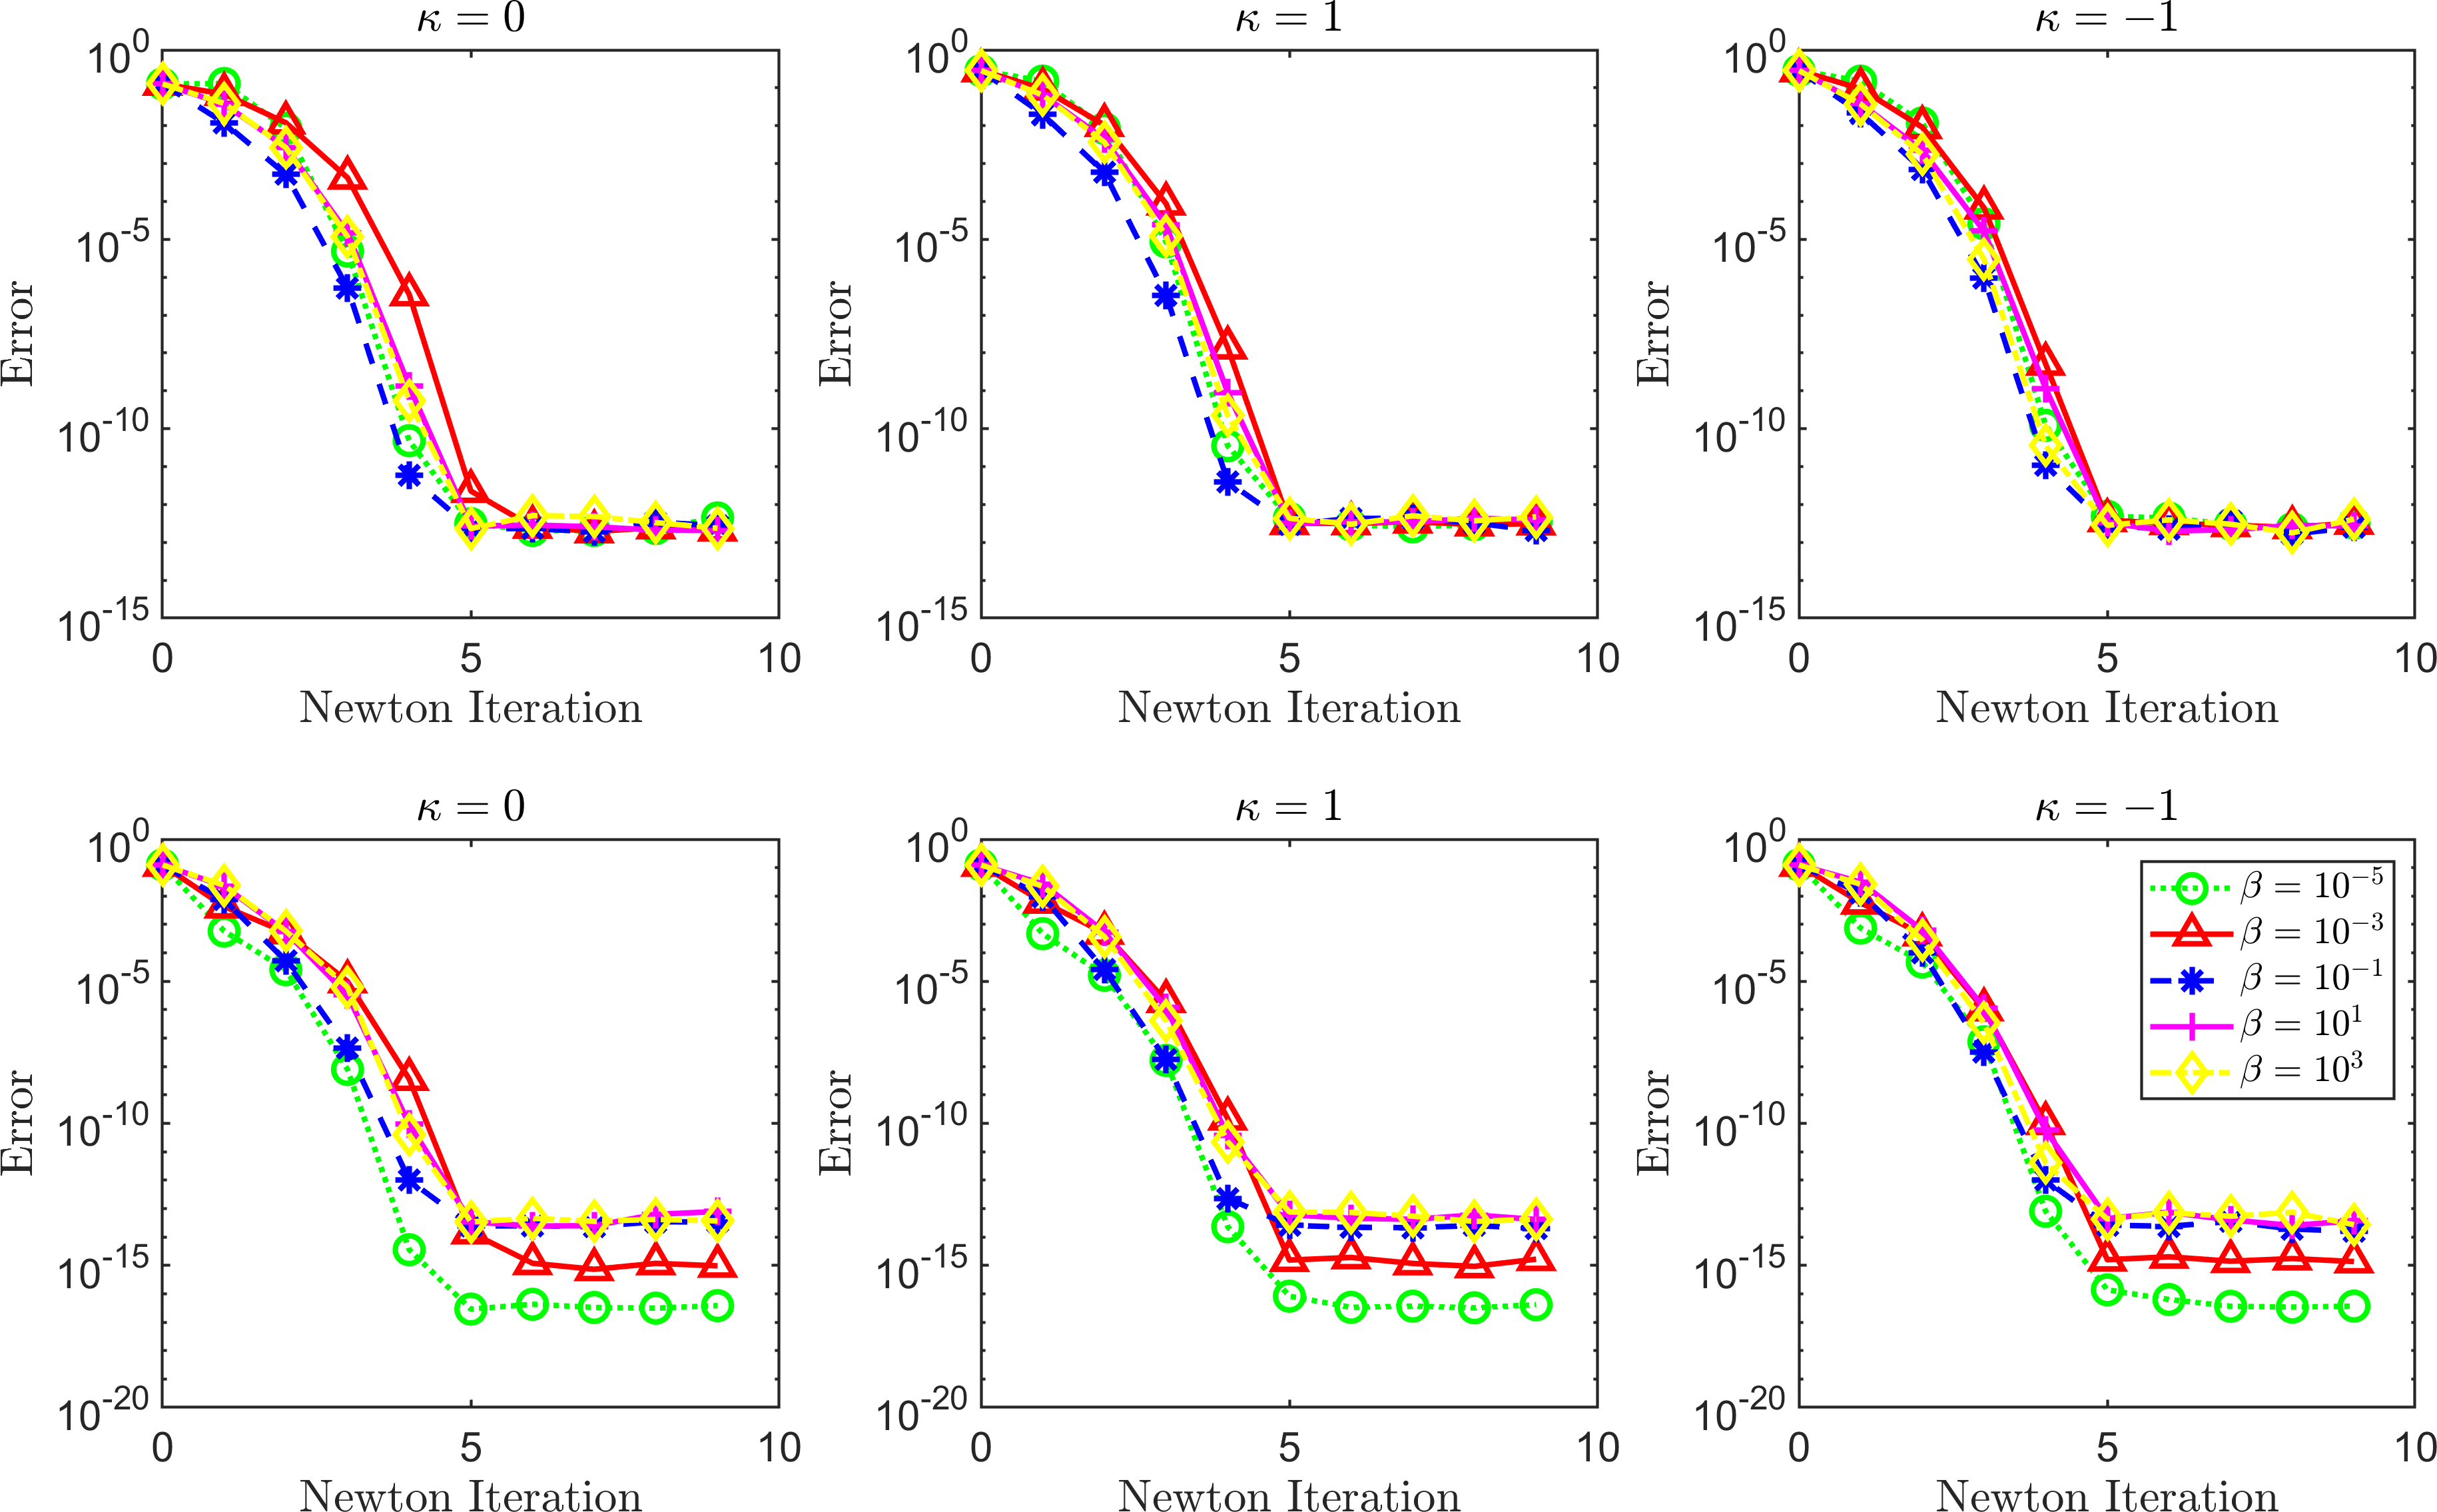
\includegraphics[scale=0.1]{SCNConvergence.png}
	\caption{Convergence of the Newton-Krylov Algorithm for no-flux source control. Top three plots show the convergence in the state variable for different $\kappa$, while the bottom plots show the convergence in the adjoint variable.} 
	\label{Con1}
\end{figure}
\begin{figure}[h]
	\centering
	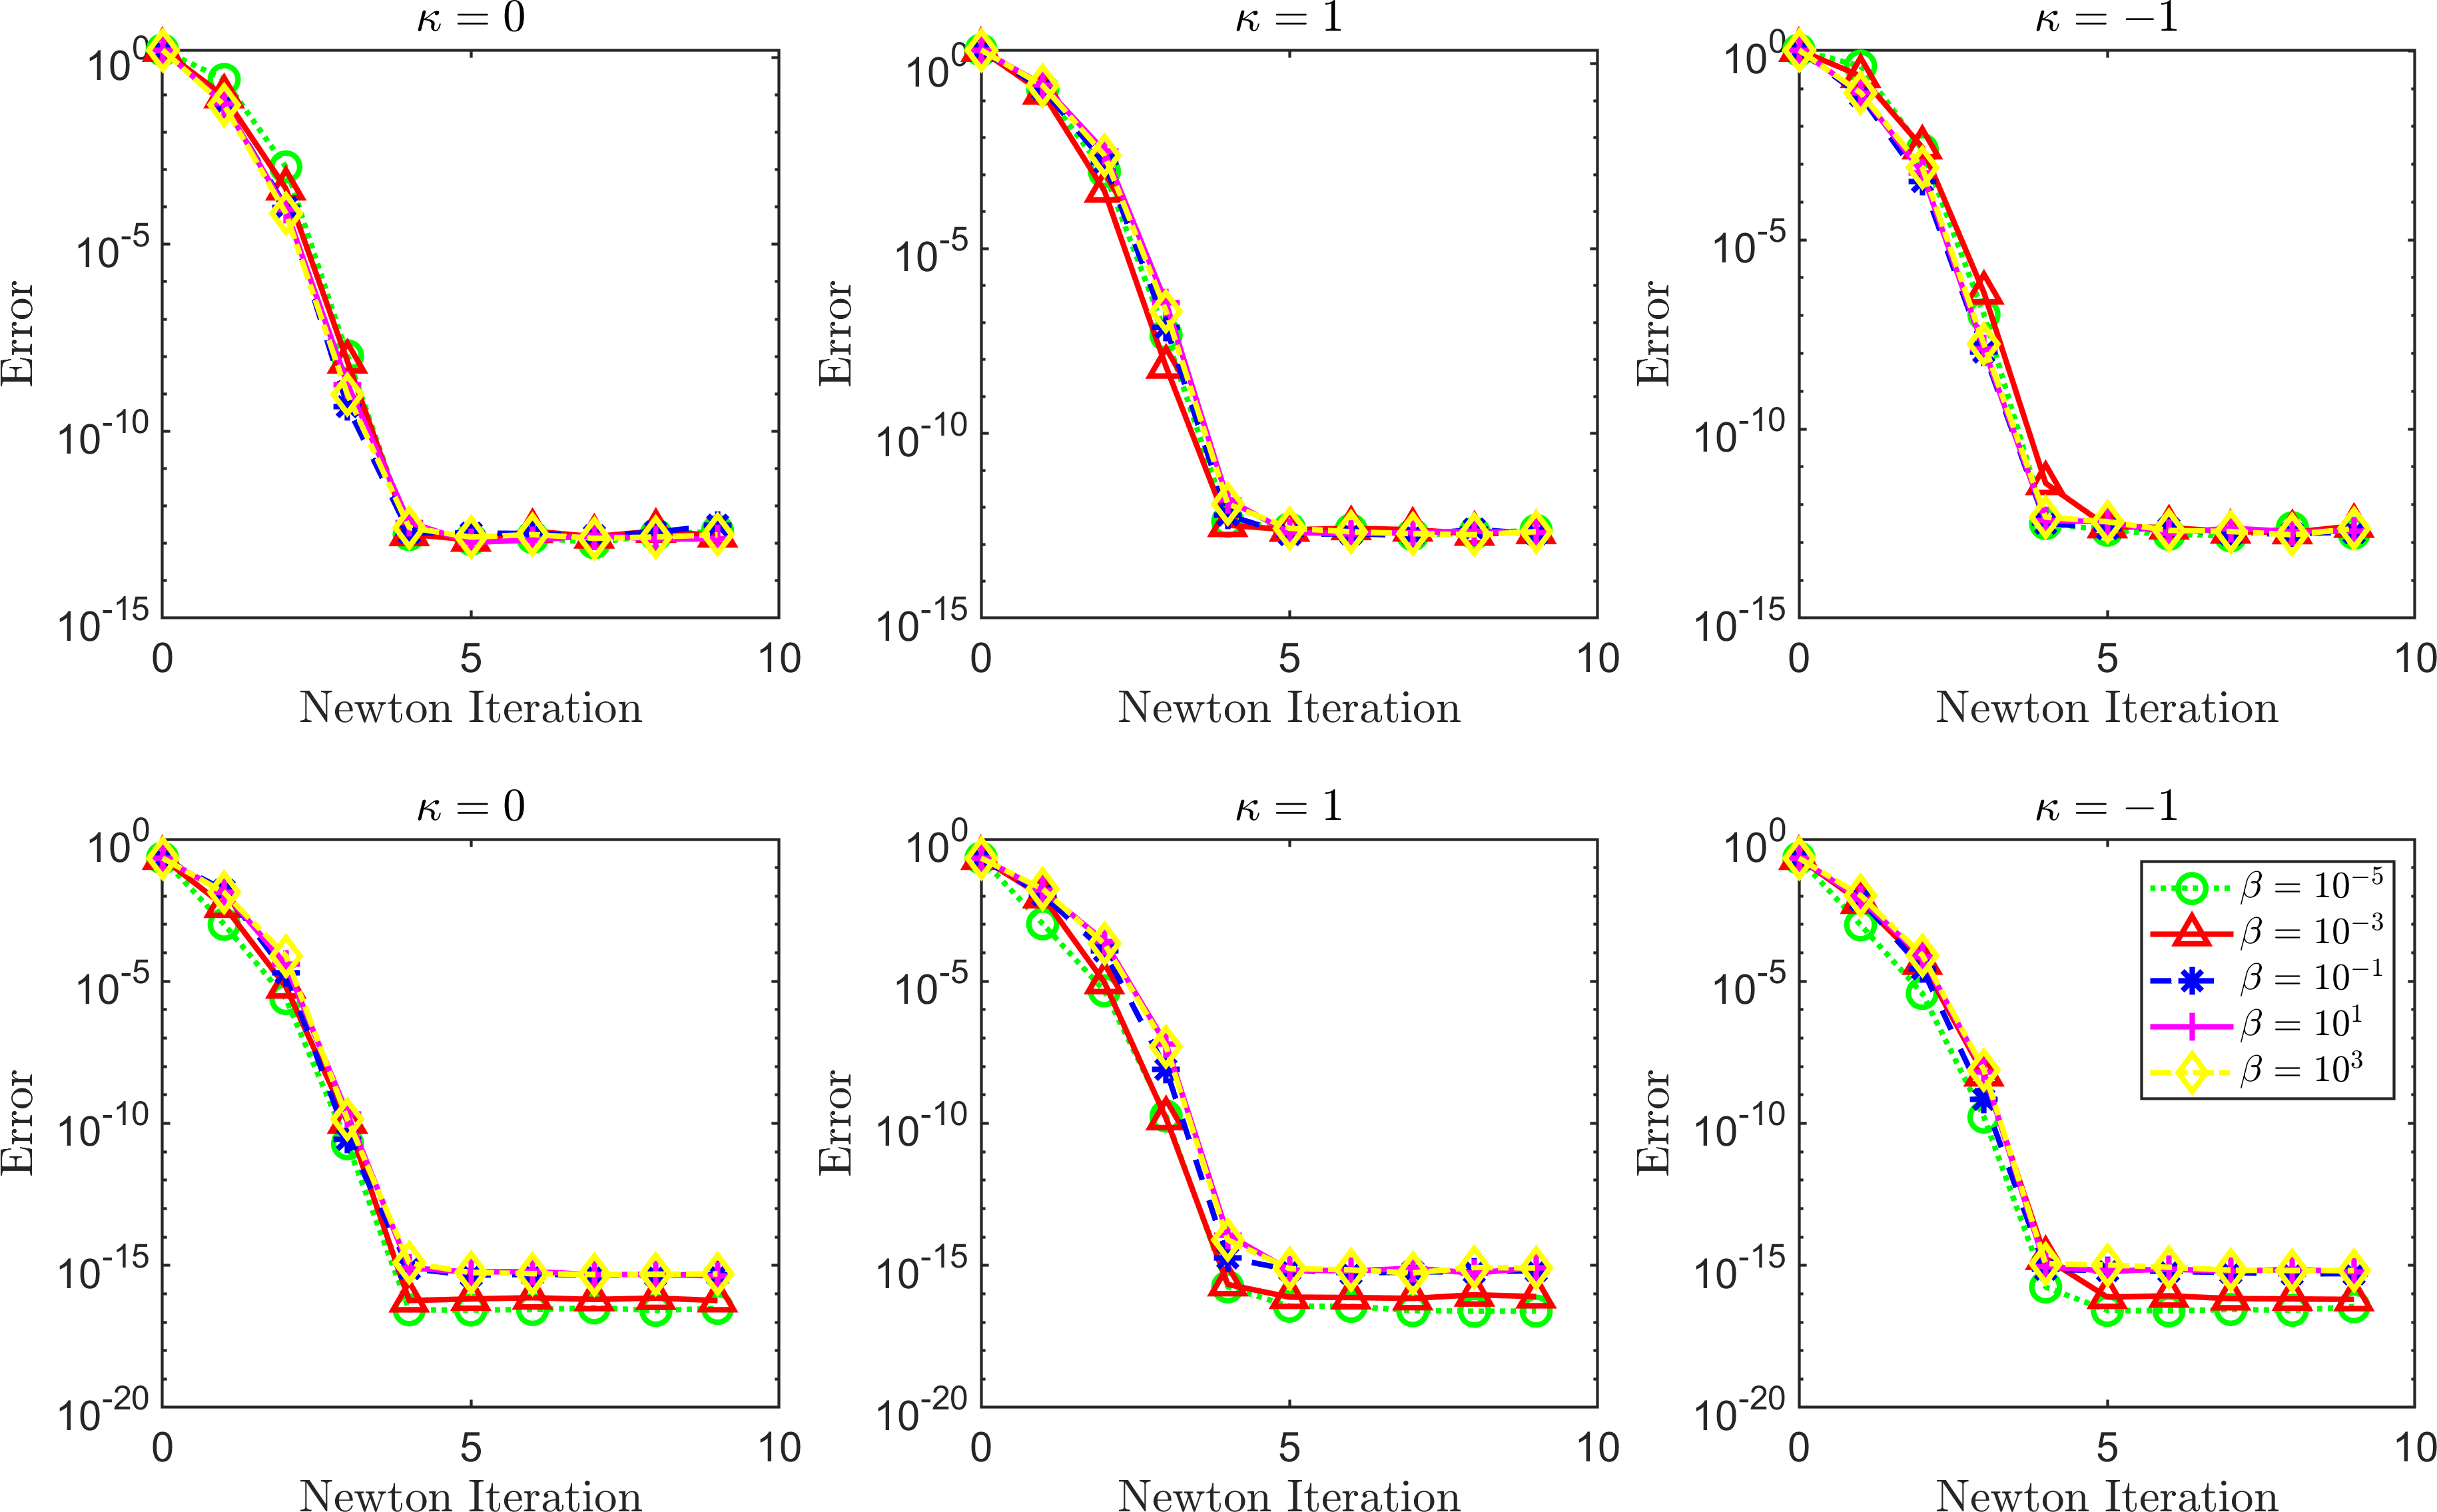
\includegraphics[scale=0.1]{SCDConvergence.png}
	\caption{Convergence of the Newton-Krylov Algorithm for Dirichlet source control. Top three plots show the convergence in the state variable for different $\kappa$, while the bottom plots show the convergence in the adjoint variable.} 
	\label{Con2}
\end{figure}
\begin{figure}[h]
	\centering
	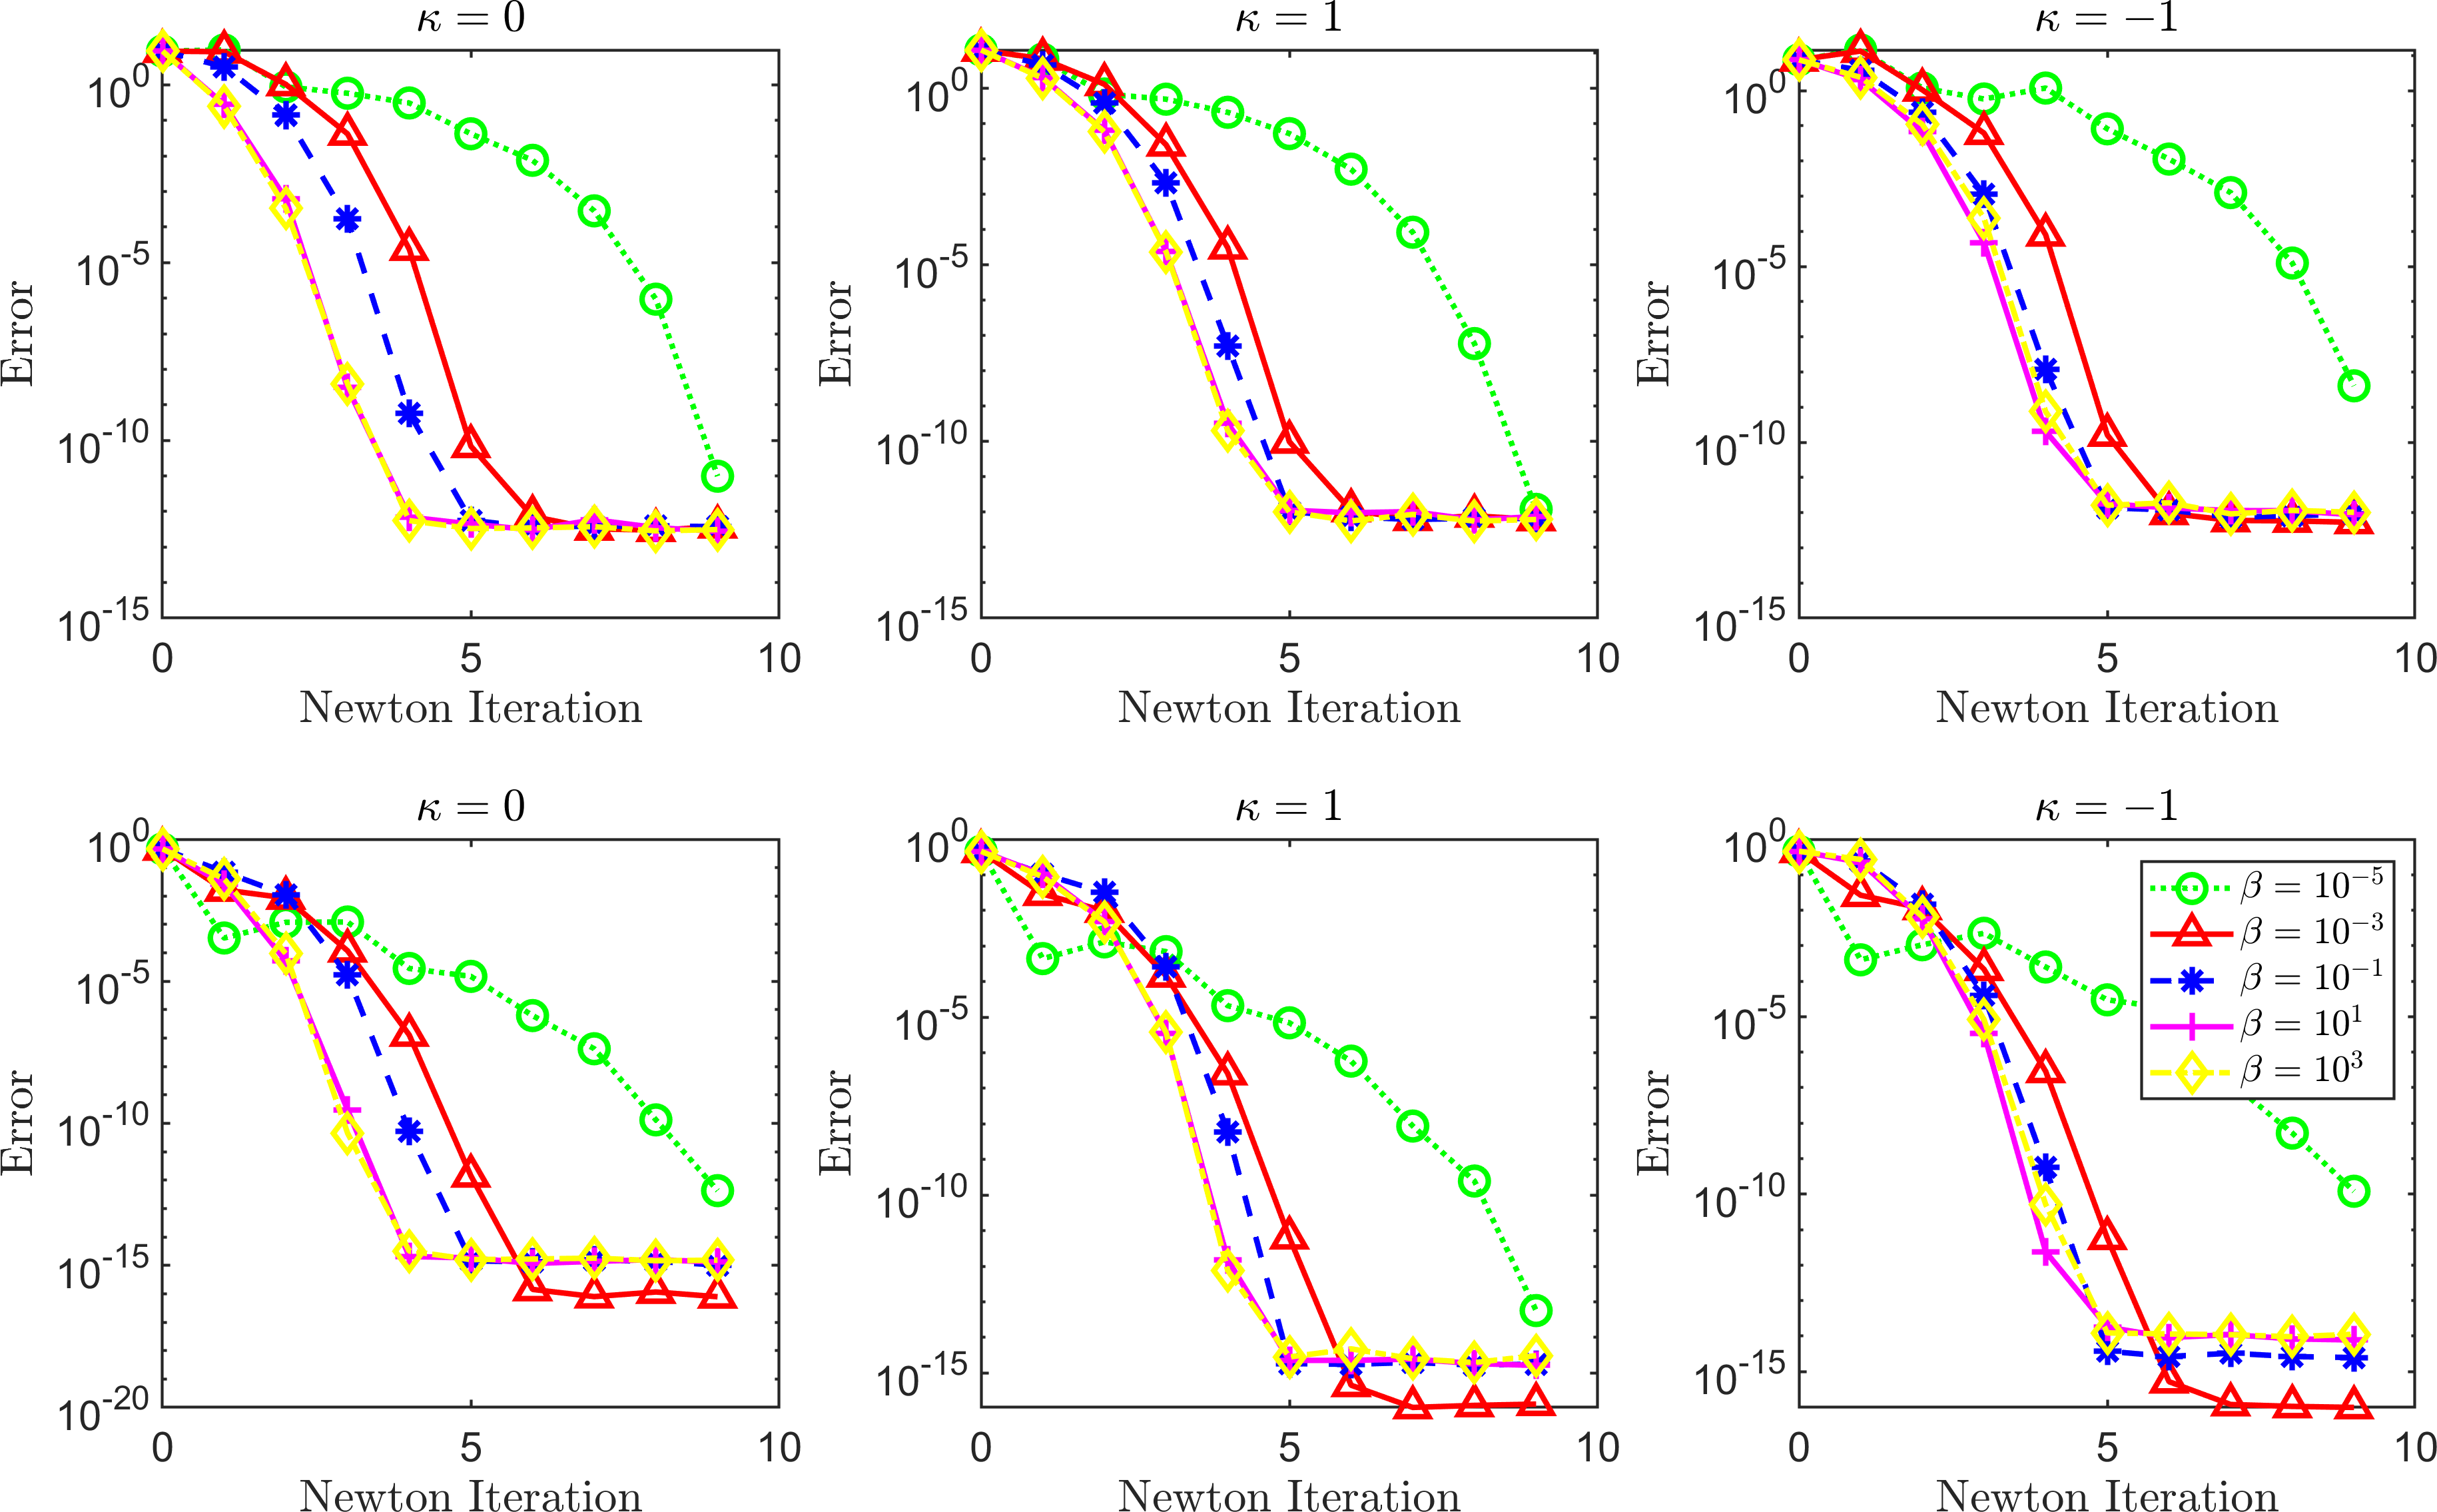
\includegraphics[scale=0.1]{FCDConvergence.png}
	\caption{Convergence of the Newton-Krylov Algorithm for Dirichlet flow control. Top three plots show the convergence in the state variable for different $\kappa$, while the bottom plots show the convergence in the adjoint variable.} 
	\label{Con3}
\end{figure}
\begin{figure}[h]
	\centering
	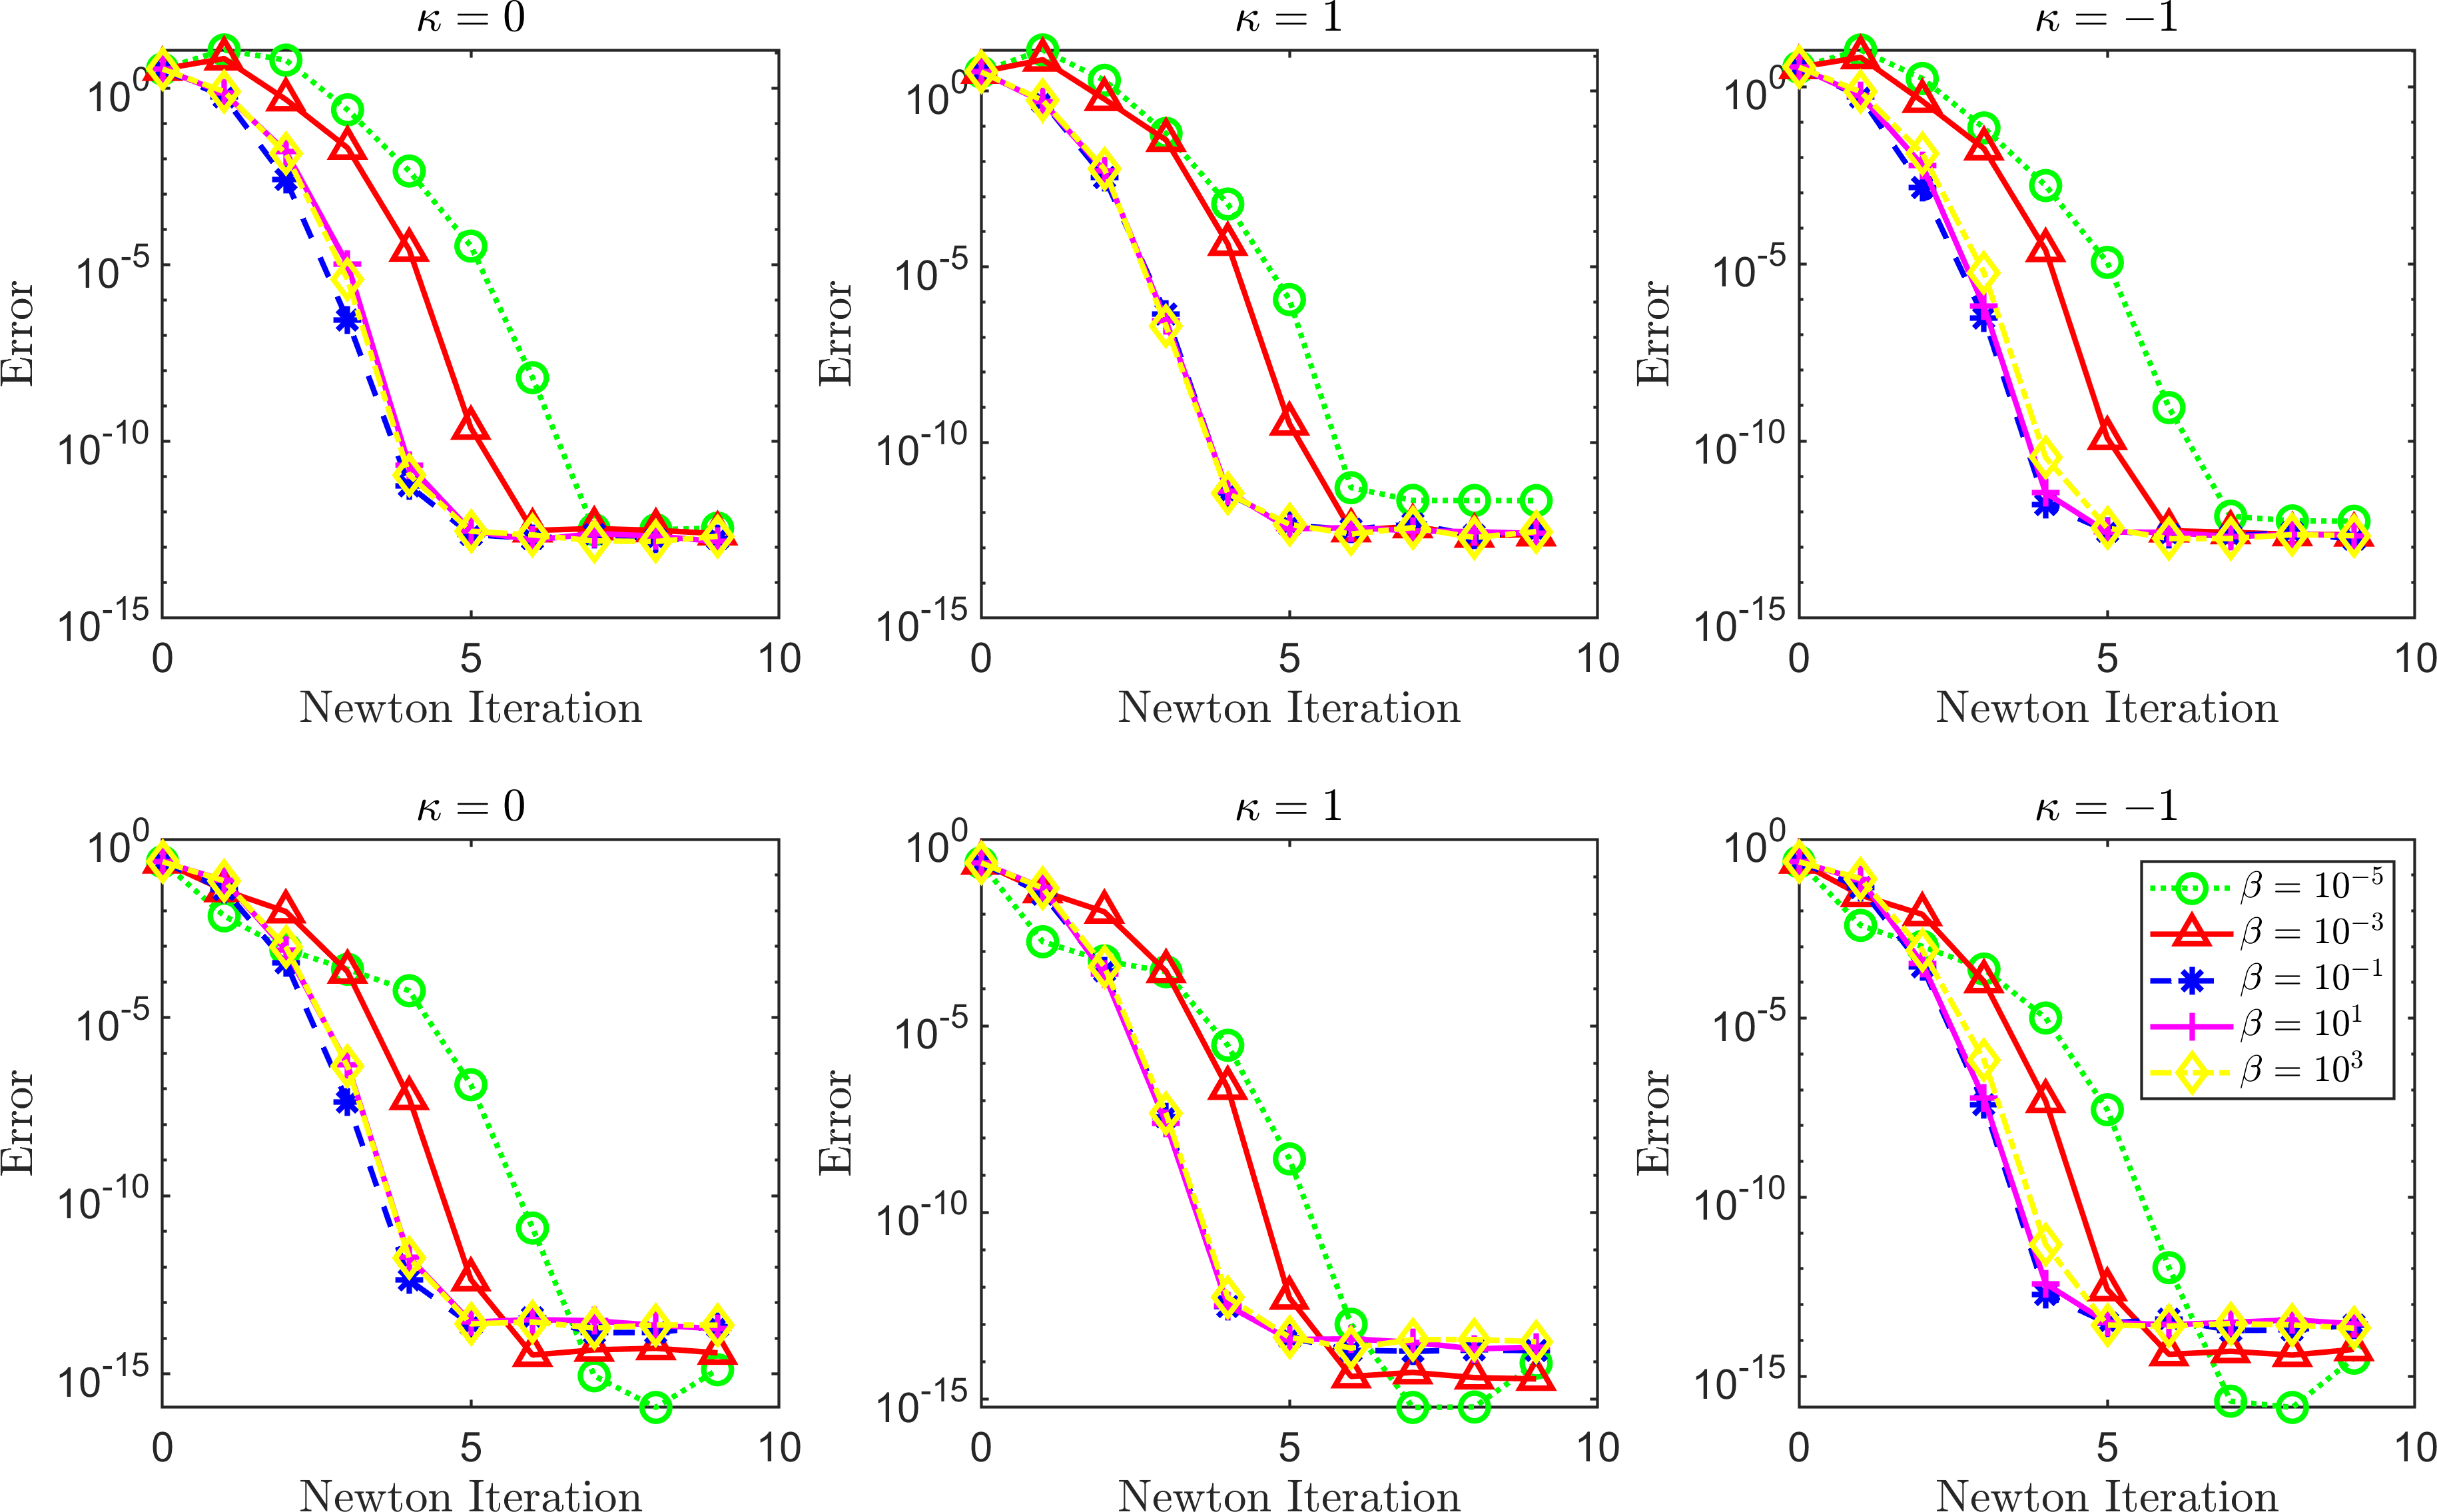
\includegraphics[scale=0.1]{FCNConvergence.png}
	\caption{Convergence of the Newton-Krylov Algorithm for no-flux flow control. Top three plots show the convergence in the state variable for different $\kappa$, while the bottom plots show the convergence in the adjoint variable.} 
	\label{Con4}
\end{figure}
	\subsection{Examples on a multishape}
	We consider the following optimal control problem:
\begin{align*}
&\mathcal{J}(\rho, \w) = \frac{1}{2}|| \rho - \widehat \rho||^2_{L_2(\Sigma)} + \frac{\beta}{2}|| \w ||^2_{L_2(\Sigma)}\\
&\text{subject to:}\\
&\frac{\partial \rho}{\partial t} = \nabla^2 \rho - \nabla (\rho \w) + \kappa \nabla \int_\Omega \rho(r) \rho(r') \K(r,r') dr'.
\end{align*}
\section*{Example 1}
The initial configuration for this example is:
\begin{align*}
&\rho_0 = \exp(-2((y_1 - 0.5 )^2 + (y_2 + 0.5)^2))\\
&\w = \mathbf 0.
\end{align*}
The target $\widehat \rho$ is set by running a forward problem with the same $\rho_0$ but with constant velocity $\w = \mathbf{1}$.
The domain for this example is a quadrilateral and a wedge and can be seen in Figure \ref{Dom1}. The tolerances are $10^{-3}/ 10^{-7}$. Per shape $N = 20$ and $n = 20$. We plot the times $2/20$, $10/20$ and $19/20$.

\begin{figure}[h]
	\centering
	\includegraphics[scale=0.6]{Dom1.png}
	\caption{Domain Example 1} 
	\label{Dom1}
\end{figure}
Choosing $\kappa = -1$, we get $J_{FW} = 0.0251$, $J_{Opt} = 0.0020$. In Figure \ref{FEx1a}, $\widehat \rho$ and corresponding $\w$ are plotted, while in Figure \ref{FEx1b}, the optimal result is displayed. Choosing $\kappa = 1$, we get $J_{FW} = 0.0176$, $J_{Opt} = 0.0020$. In Figure \ref{FEx1c}, $\widehat \rho$ and corresponding $\w$ are plotted, while in Figure \ref{FEx1d}, the optimal result is displayed. It can be seen that while the attractive particles clump in the middle, the repulsive particles are clustered at the boundaries.
\begin{figure}[h]
	\centering
	\includegraphics[scale=0.6]{FW1n1.png}
	\caption{Example 1, $\widehat \rho$, $\kappa = -1$} 
	\label{FEx1a}
\end{figure}
\begin{figure}[h]
	\centering
	\includegraphics[scale=0.6]{Opt1n1.png}
	\caption{Example 1, optimal $\rho$ and $\w$, $\kappa = -1$} 
	\label{FEx1b}
\end{figure}

\begin{figure}[h]
	\centering
	\includegraphics[scale=0.6]{FW11.png}
	\caption{Example 1, $\widehat \rho$, $\kappa = 1$} 
	\label{FEx1c}
\end{figure}
\begin{figure}[h]
	\centering
	\includegraphics[scale=0.6]{Opt11.png}
	\caption{Example 1, optimal $\rho$, $\w$, $\kappa = 1$} 
	\label{FEx1d}
\end{figure}
(Note to self: this corresponds to Test10/ Example5a in code.)
\section*{Example 2}
As initial configuration we choose:
\begin{align*}
&\rho_0 = \exp(-2((y_1 - 0.5 )^2 + (y_2 + 0.5)^2))\\
&\w = \mathbf{0}.
\end{align*}	
The target is a forward problem run with the same $\rho_0$ but with a constant background flow $\w = \mathbf{5}$. We run the problem up to time $2$, as opposed to time $1$ as usual. This is more stable than increasing the strength of the background flow. We still plot the time points $2/20$, $10/20$ and $19/20$. The domain of the problem is a channel, see Figure \ref{Dom2}.
\begin{figure}[h]
	\centering
	\includegraphics[scale=0.6]{Dom2.png}
	\caption{Domain Example 2} 
	\label{Dom2}
\end{figure}


Choosing $\kappa = -1$, we get $J_{FW} =  0.4111$, $J_{Opt} =  0.0807$. In Figure \ref{FEx2a}, $\widehat \rho$ and corresponding $\w$ are plotted, while in Figure \ref{FEx2b}, the optimal result is displayed. Choosing $\kappa = 1$, we get $J_{FW} =  0.3501$, $J_{Opt} =  0.0821$. In Figure \ref{FEx2c}, $\widehat \rho$ and corresponding $\w$ are plotted, while in Figure \ref{FEx2d}, the optimal result is displayed. Again, the difference between attractive and repulsive interaction is clearly displayed by the clustering of the particles in the channel. (Note to self: this is test 11a and Example4a) 
\begin{figure}[h]
	\centering
	\includegraphics[scale=0.3]{FW2n1.png}
	\caption{Example 2, $\widehat \rho$, $\kappa = -1$} 
	\label{FEx2a}
\end{figure}
\begin{figure}[h]
	\centering
	\includegraphics[scale=0.3]{Opt2n1.png}
	\caption{Example 2, optimal $\rho$ and $\w$, $\kappa = -1$} 
	\label{FEx2b}
\end{figure}

\begin{figure}[h]
	\centering
	\includegraphics[scale=0.3]{FW21.png}
	\caption{Example 2, $\widehat \rho$, $\kappa = 1$} 
	\label{FEx2c}
\end{figure}
\begin{figure}[h]
	\centering
	\includegraphics[scale=0.3]{Opt21.png}
	\caption{Example 2, optimal $\rho$ and $\w$, $\kappa = 1$} 
	\label{FEx2d}
\end{figure}







	
\section*{Example 3}
As initial configuration we choose:
\begin{align*}
&\rho_0 = \exp(-2((y_1 + 1)^2 + (y_2 + 0.3)^2))\\
&\w = \mathbf{0}.
\end{align*}	
The target is a forward problem run with the same $\rho_0$ but with a background flow of constant one running along the domain. This and the domain of the problem can be seen in Figure \ref{Dom3}.
\begin{figure}[h]
	\centering
	\includegraphics[scale=0.4]{Dom3.png}
	\includegraphics[scale=0.4]{Flow3.png}
	\caption{Domain and Flow Example 3} 
	\label{Dom3}
\end{figure}	
	
Choosing $\kappa = -1$, we get $J_{FW} = 0.0184$, $J_{Opt} = 9.5312 \times 10^{-4}$. In Figure \ref{FEx3a}, $\widehat \rho$ and corresponding $\w$ are plotted, while in Figure \ref{FEx3b}, the optimal result is displayed.
\begin{figure}[h]
	\centering
	\includegraphics[scale=0.3]{FW3n1.png}
	\caption{Example 3, $\widehat \rho$, $\kappa = -1$} 
	\label{FEx3a}
\end{figure}
\begin{figure}[h]
	\centering
	\includegraphics[scale=0.3]{Opt3n1.png}
	\caption{Example 3, optimal $\rho$ and $\w$, $\kappa = -1$} 
	\label{FEx3b}
\end{figure}	
	
Choosing $\kappa = 1$, we get $J_{FW} = 0.0150$, $J_{Opt} = 0.0010$. In Figure \ref{FEx3c}, $\widehat \rho$ and corresponding $\w$ are plotted, while in Figure \ref{FEx3d}, the optimal result is displayed. It is very obvious here how different the attractive and repulsive particles behave in this channel. It seems that the repulsive particles are clustering more on the sides and at the end of the channel, while the attractive particles are closer to the middle.
\begin{figure}[h]
	\centering
	\includegraphics[scale=0.3]{FW31.png}
	\caption{Example 3, $\widehat \rho$, $\kappa = 1$} 
	\label{FEx3c}
\end{figure}
\begin{figure}[h]
	\centering
	\includegraphics[scale=0.3]{Opt31.png}
	\caption{Example 3, optimal $\rho$ and $\w$, $\kappa = 1$} 
	\label{FEx3d}
\end{figure}	
	
	
	
	
	
	
	\section{Industrial Motivation Revisited}









    \section{Sedimentation}
    
	\subsection{Background DDFT}
		\begin{itemize}
			\item Derivation of the extra term from SPT, explain FMT, etc. 
			\item A little literature review
			\item Comparison of simulations to Archer?
		\end{itemize}
	We are interested in modelling sedimentation processes. In order to achieve this, the advection-diffusion equation with mean-field interaction term has to be modified to include an approximation to volume exclusion. Archer and Malijevs\'y \cite{ArcherSed1} have achieved this using the following model to describe sedimentation processes. 
The modelling equations are:
\begin{align*}
	&\frac{\partial \rho}{\partial t^*} = \Gamma\nabla \cdot \left(  \rho \nabla \frac{\delta F[\rho]}{\delta \rho} \right) ,
\end{align*}
where $\Gamma$ is the diffusion coefficient. 	
We can rescale this equation as done in \cite{ArcherSed1} using the relationship $t = t^*/ \tau_B$, where $\tau_B = \beta \sigma^2 / \Gamma$ is the Brownian time scale.
Applying this rescaling we get:
\begin{align}\label{Eq1}
	&\frac{\partial \rho}{\partial t} = \beta \sigma^2\nabla \cdot \left(  \rho \nabla \frac{\delta F[\rho]}{\delta \rho} \right).
\end{align}
The free energy functional considered in \cite{ArcherSed1} is:
\begin{align*}
	F[\rho] &= \frac{1}{\beta} \int \rho (\ln \Lambda^2 \rho - 1) + f_{HDA} dr + \frac{1}{2}\int \int \rho(r) \rho(r') V_2(|r - r'|) dr dr' + \int \rho V_{ext} dr,
\end{align*}
where $f_{HDA}$ the approximate free energy density describing the volume exclusion through hard disks. The external potential is defined as:
\begin{align*}
	V_{ext} &= c y, \quad \text{for } \quad 0 < y < L,
\end{align*}
where $c$ a constant and $L$ is the height of a rectangular domain. Outside these bounds $V_{ext} = \infty$. 
Furthermore, we have the pair potential:
\begin{align*}
	V_2 = exp(-r/\sigma),
\end{align*}
where $\sigma$ is the particle diameter of the hard sphere particle.


\subsubsection{The Hard Disk Approximation}
The part of the free energy functional, which accounts for the hard disk approximation, is:
\begin{align*}
	F_{HDA}[\rho] &= \frac{1}{\beta} \int  f_{HDA} dr = \frac{1}{\beta} \int   -  \rho - \rho \ln(1 - \eta) + \frac{\rho}{1 - \eta} dr,
\end{align*}
where $\eta = a \rho = \frac{\pi \sigma^2}{4} \rho$.
This can be thought of as the bulk fluid, one species, two dimensional approximation of Fundamental Measure Theory (FMT)  \cite{RosenfeldFMT}, which is a Density Functional Theory for hard sphere mixtures. The basis of this theory is that the excess free energy functional is of the form:
\begin{align*}
	\beta F_{ex}[{\rho_i}] = \int \Phi({n_\alpha(r')})d^3r',
\end{align*} 
where $i$ is the species count and $\Phi$ is a function of the weighted densities $n_\alpha$. By now there are many different versions of $\Phi$, yielding approximations of $F_{ex}$ with different limitations, see \cite{Roth_2010FMTReview}. Rosenfeld's original version is defined as:
	\begin{align*}
	\Phi = -n_0 \ln(1-n_3) + \frac{n_1 n_2 - \mathbf{n_1} \cdot \mathbf{n_2}}{1-n_3} + \frac{n_2^3 - 3n_2 \mathbf{n_2} \cdot \mathbf{n_2}}{24 \pi (1-n_3)^2}.
	\end{align*}
The weighted densities for $\nu$ species are:
	\begin{align} \label{eqn:WeightedDensities}
		n_\alpha (r) = \sum_{i=1}^\nu \int \rho_i(r') \omega_\alpha^i(r -r').
	\end{align}
The weight functions chosen by Rosenfeld are:
\begin{align*}
	&\omega_3^i = \Theta(R_i -r),\quad \omega_2^i = \delta(R_i -r),\quad \mathbf{\omega_2^i} = \frac{\mathbf r}{r}\delta (R_i -r),\quad \\
	&\omega_1^i = \omega_2^i/(4 \pi R_i), \quad \omega_0^i = \omega_2^i/(4\pi R_i^2), \quad \mathbf{\omega_1^i} = \mathbf{\omega_2^i}/(4 \pi R_i),
\end{align*}
where $R_i$ is the radius of the excluded volume, $\Theta$ is the Heaviside function and $\delta$ is the delta function. Integrating over $\omega_\alpha$, with $\alpha = 0,1,2,3$, we get the fundamental measures of a sphere: volume, surface area, radius and the Euler characteristic \cite{Roth_2010FMTReview} \cite{RosenfeldFMT}.
\\
Based on this theory for three dimensional spheres and the fact that the theory for hard rods is known exactly \cite{Percus1976}, Rosenfeld derived a version of this approach for two dimensional hard disks \cite{Rosenfeld2DInterp}. However, some additional approximations have to be made when choosing the weighted densities, which is not necessary in one and three dimensions. The resulting equation is:
\begin{align*}
	\Phi = - n_0 \ln(1-n_3) + \frac{1}{4 \pi} \frac{n_2 n_2}{1-n_3} + \frac{1}{4 \pi} \frac{\mathbf{n_2} \cdot \mathbf{n_2}}{1-n_3}.
\end{align*}
\\
In the uniform limit, for one particle species, we get that:
\begin{align*}
	n_0 = \rho, \quad n_2 = 2 \pi R \rho, \quad n_3 = \pi R^2 \rho,
\end{align*}
by solving the integrals in \eqref{eqn:WeightedDensities}, using spherical polar coordinates, with $\rho = \rho_{\text{bulk}}$, a constant. 
Substituting this in the 2D version of $\Phi$ gives:
\begin{align*}
	\Phi = - \rho \ln (1- \pi R^2 \rho) + \frac{1}{4 \pi} \frac{4\pi^2 R^2 \rho^2}{1 - \pi R^2 \rho} + \frac{1}{4 \pi}\frac{\mathbf{n_2} \cdot \mathbf{n_2}}{1 - \pi R^2 \rho},
\end{align*}
where $\mathbf{n_2} = \mathbf 0$ in the uniform limit, since the corresponding equation in \eqref{eqn:WeightedDensities} is an integral over an odd function.
Noting that $R = \sigma/2$ and $\eta = \pi \sigma^2 \rho /4$, we get that:
\begin{align} \label{eqn:SPTFunctional2D}
	\Phi = - \rho \ln (1- \eta) + \frac{\rho \eta}{1 - \eta} = \rho \left(-\ln(1-\eta) + \frac{1}{1- \eta} -1 \right).
\end{align} 
This expression for the free energy for the bulk fluid is the same as derived by scaled particle theory (SPT) \cite{Reiss1959}, \cite{Reiss1960}, \cite{Helfand1961}, which also coincides with the Percus-Yevic compressibility equation \cite{PercusYevick1}, as detailed in \cite{RosenfeldSPT}.
While the SPT approximation \eqref{eqn:SPTFunctional2D} and its three-dimensional equivalent are used in classical DFT, see \cite{DFTWinkelmann2001}, \cite{DFTRoth1}, \cite{DFTRoth2}, \cite{DFTGonzalez1997}, \cite{DFTCuesta2008}, \cite{DFTLoewen2002}, and other statistical mechanics approaches, see \cite{GrafLoewen1999}, \cite{DuBois2002}, \cite{Chamoux1998}, \cite{Chamoux1996}, in dynamical DFT it is not commonly applied and only the work of Archer et al. \cite{ArcherSed1}, \cite{ArcherSed2008}, \cite{ArcherSed2011}, \cite{ArcherSed2013}, is known to us in this context.

\subsubsection{Deriving the equation of motion}
Since we are interested in the equation of motion, we need to calculate $ \nabla \cdot \left(\rho \nabla \frac{\delta F_{HDA}[\rho]}{\delta \rho} \right)$. We combine $F_{HDA}$ and $F_{ID} = \int_\Omega \rho (\ln \Lambda^2 \rho - 1) dr$ here so that we have:
\begin{align*}
	F_{N} = F_{HDA} + F_{ID}.
\end{align*}
Taking the functional derivative of $F_{N}$ gives:
\begin{align*}
	\frac{\delta F_{N}[\rho]}{\delta \rho} &= \frac{1}{\beta} \bigg(1 + \ln \rho + \Lambda^2 -2 - \ln(1-\eta) + a \frac{\rho}{1 - \eta} + \frac{1}{1 - \eta} + a \frac{\rho}{(1 - \eta)^2}  \bigg)\\
	&= \frac{1}{\beta} \bigg(1 + \ln \rho + \Lambda^2 -2 - \ln(1-\eta) + \frac{1}{(\eta - 1)^2} - \frac{1}{\eta - 1}  - 1\bigg)\\
	&= \frac{1}{\beta} \bigg( \ln \rho + \Lambda^2 - 2 - \ln(1-\eta) - \frac{\eta - 2}{(\eta - 1)^2}  \bigg),
\end{align*}
using partial fractions. Then:
\begin{align*}
	\nabla \frac{\delta F_{N}[\rho]}{\delta \rho} &= \frac{1}{\beta} \bigg( \nabla\ln \rho + \nabla(\Lambda^2 - 2) - \nabla\ln(1-\eta) - \nabla\frac{\eta - 2}{(\eta - 1)^2}  \bigg)\\
	& = \frac{1}{\beta} \bigg( \frac{\nabla \rho}{\rho} - \frac{\nabla( 1- \eta)}{1 - \eta} - \nabla\frac{\eta - 2}{(\eta - 1)^2}  \bigg)\\
	& = \frac{1}{\beta} \bigg( \frac{\nabla \rho}{\rho} + \frac{\nabla \eta}{1 - \eta} - \nabla\frac{\eta - 2}{(\eta - 1)^2}  \bigg).
\end{align*}
Then multiplying by $\rho$ gives:
\begin{align*}
	\rho \nabla \frac{\delta F_{N}[\rho]}{\delta \rho} &= \frac{1}{\beta} \bigg( \nabla \rho +   \frac{\rho \nabla \eta}{1 - \eta} - \rho \nabla\frac{\eta - 2}{(\eta - 1)^2}  \bigg)\\
	&= \frac{1}{\beta} \bigg( \nabla \rho +   \frac{\eta\nabla \rho}{1 - \eta} - \rho \nabla\frac{\eta - 2}{(\eta - 1)^2}  \bigg)\\
	&= \frac{1}{\beta} \bigg( \nabla \rho + \frac{\nabla \rho}{1 - \eta} - \nabla \rho - \rho \nabla\frac{\eta - 2}{(\eta - 1)^2}  \bigg)\\
	&= \frac{1}{\beta} \bigg(  \frac{\nabla \rho}{1 - \eta}  - \rho \nabla\frac{\eta - 2}{(\eta - 1)^2}  \bigg).
\end{align*}
Finally we take the divergence:
\begin{align*}
	\nabla \cdot \bigg(\rho \nabla \frac{\delta F_{N}[\rho]}{\delta \rho}\bigg) &= \frac{1}{\beta} \bigg( \nabla  \cdot \left(  \frac{\nabla \rho}{1 - \eta} \right) - \nabla  \cdot \left(\rho \nabla\frac{\eta - 2}{(\eta - 1)^2} \right) \bigg)\\
	&= \frac{1}{\beta} \bigg( \frac{\nabla^2 \rho}{1 - \eta} +  \nabla \rho \cdot \nabla \frac{1}{1 - \eta} - \nabla \rho \cdot \nabla \frac{\eta - 2}{(\eta - 1)^2} - \rho \nabla^2\frac{\eta - 2}{(\eta - 1)^2} \bigg)\\
	&= \frac{1}{\beta} \bigg( \frac{\nabla^2 \rho}{1 - \eta} +  \nabla \rho \cdot \nabla \frac{(3- 2 \eta)}{(1 - \eta)^2}  - \rho \nabla^2\frac{\eta - 2}{(\eta - 1)^2} \bigg).
\end{align*}
	
	\subsection{OCP}
		\begin{itemize}
			\item State possible OCPs
			\item Derive Optimality Conditions
			\item Here add Periodic BCs and time-independent control
			\item In the future maybe also the things on curl free control
		\end{itemize}
	One optimal control problem to consider is:
\begin{align}\label{eq:OCP1}
	&J = \frac{1}{2}\int_0^T \int_\Omega (\rho - \widehat \rho)^2 dr dt + \frac{\beta}{2} \int_0^T\int_\Omega \w(r)^2 dr \notag\\
	&\text{subject to:}\\
	&\frac{\partial \rho}{\partial t} = \beta \sigma^2 \bigg( \nabla \cdot (\rho \nabla V_{ext}) - \nabla (\rho \w) + \nabla \cdot \left(\rho \nabla \frac{\delta F_{N}[\rho]}{\delta \rho}\right) + \kappa \int_\Omega \rho(r) \rho(r') \K(r,r')dr\bigg), \notag
\end{align}
where $\K(r,r') = \nabla V_2$.
We consider the terms of the PDE and the boundary conditions separately here.
\subsubsection{Calculating Frech\'et Derivatives}
In order to derive the optimalty conditions for the above OCP, we need to calculate the Frech\'et derivatives of the following terms:
\begin{align*}
	\nabla \cdot \bigg(\rho \nabla \frac{\delta F_{N}[\rho]}{\delta \rho}\bigg)
	&= \frac{1}{\beta} \bigg( \frac{\nabla^2 \rho}{1 - \eta} +  \nabla \rho \cdot \nabla \frac{(3- 2 \eta)}{(1 - \eta)^2}  - \rho \nabla^2\frac{\eta - 2}{(\eta - 1)^2} \bigg),
\end{align*}
where $\eta = a \rho$ and $a = \pi \sigma^2 /4$.
Consider:
\begin{align*}
	F_1(\rho) &= \nabla^2 \rho \frac{1}{1- a\rho},\\
	F_2(\rho) &= \nabla \rho \cdot \nabla \left(\frac{3-2a\rho}{(1-a\rho)^2}\right),\\
	F_3(\rho) &= \rho \nabla^2 \left(\frac{a\rho -2}{(a\rho -1)^2}\right).
\end{align*}
Then
\begin{align*}
	F_1(\rho + h) - F_1(\rho) &= \nabla (\rho +h) \frac{1}{1- a(\rho +h)} - \nabla \rho \frac{1}{1- a\rho}.
\end{align*}
Using the expansion: 
\begin{align*}
	\frac{1}{c - x} = \frac{1}{c} + \frac{1}{c^2}x + O(x^2),
\end{align*}
where $c = 1- a \rho$, we get:
\begin{align*}
	F_1(\rho + h) - F_1(\rho) &= \nabla^2 (\rho +h) \left(\frac{1}{1- a\rho} + \frac{a}{(1- a\rho)^2}h \right)- \nabla^2 \rho \frac{1}{1- a\rho}\\
	&= \nabla^2 h \left(\frac{1}{1- a\rho} \right) + \nabla^2 \rho \left(\frac{a}{(1- a\rho)^2}h\right),
\end{align*}
not considering higher order terms of $h$.
For $F_2$ we consider the expansion:
\begin{align*}
	\frac{1}{(c-x)^2} = \frac{1}{c^2} + \frac{2}{c^3}x + O(x^2),
\end{align*}
and get:
\begin{align*}
	F_2(\rho+h) - F_2(\rho) &= \nabla (\rho +h) \cdot \nabla \left(\frac{3-2a(\rho +h)}{(1-a(\rho+h))^2}\right) -\nabla \rho \cdot \nabla \left(\frac{3-2a\rho}{(1-a\rho)^2}\right) \\
	&= \nabla (\rho +h) \cdot \nabla \left(\frac{3-2a(\rho +h)}{(1-a\rho)^2} + \frac{3-2a(\rho +h)}{(1-a\rho)^3} 2ah \right) -\nabla \rho \cdot \nabla \left(\frac{3-2a\rho}{(1-a\rho)^2}\right)\\
	&=\nabla h \cdot \nabla \left(\frac{3-2a\rho}{(1-a\rho)^2} \right) + \nabla \rho \cdot \nabla \left(h\left(\frac{-2a }{(1-a\rho)^2} + \frac{6a-4a^2  \rho}{(1-a\rho)^3}  \right)\right)\\
	& = \nabla h \cdot \nabla \left( \frac{3-2a\rho}{(1-a\rho)^2} \right) + \left(\nabla h \cdot \nabla \rho \right) \left( \frac{-2a }{(1-a\rho)^2} + \frac{6a-4a^2  \rho}{(1-a\rho)^3}  \right) \\
	&+ h \nabla \rho \cdot \nabla \left(\frac{-2a }{(1-a\rho)^2} + \frac{6a-4a^2  \rho}{(1-a\rho)^3}  \right).
\end{align*}

Finally, we have:
\begin{align*}
	F_3(\rho+h) - F_3(\rho) &= (\rho +h) \nabla^2 \left(\frac{a(\rho +h) -2}{(a(\rho +h) -1)^2}\right) -\rho \nabla^2 \left(\frac{a\rho -2}{(a\rho -1)^2}\right)\\
	&=  (\rho +h) \nabla^2 \left(\frac{a(\rho +h) -2}{(1-a\rho)^2} + \frac{a(\rho +h) -2}{(1-a\rho)^3}2ah \right) -\rho \nabla^2 \left(\frac{a\rho -2}{(a\rho -1)^2}\right)\\
	&= h \nabla^2 \left(\frac{a\rho -2}{(a\rho -1)^2}\right) + \rho \nabla^2  \left(h\left(\frac{a }{(1-a\rho)^2} + \frac{2a^2\rho -4a}{(1-a\rho)^3} \right)\right)\\
	&= h \nabla^2 \left(\frac{a\rho -2}{(a\rho -1)^2}\right) + \rho  \left(\frac{a }{(1-a\rho)^2} + \frac{2a^2\rho -4a}{(1-a\rho)^3} \right)\nabla^2 h \\
	&+ 2 \rho \nabla \left(\frac{a }{(1-a\rho)^2} + \frac{2a^2\rho -4a}{(1-a\rho)^3} \right) \cdot \nabla h + \rho h \nabla^2  \left(\frac{a }{(1-a\rho)^2} + \frac{2a^2\rho -4a}{(1-a\rho)^3} \right).\\
\end{align*}
\subsubsection{Adjoint Equation}
In order to derive the adjoint equation, we need to consider the Lagrangian of the above OCP and take the derivative with respect to $\rho$. Given that most of the analysis has been done in a different chapter, we only consider the terms derived from $F_{N}$.
The Frech\'et derivatives of the relevant terms have been taken and are combined to give:
\begin{align*}
	\mathcal{L}_\rho(\rho,\w,q)h &= ... -\frac{1}{\beta}\int_0^T \int_\Omega q \nabla^2 h \left(\frac{1}{1- a\rho} \right) + q\nabla^2 \rho \left(\frac{a}{(1- a\rho)^2}h\right)\\
	&+ q\nabla h \cdot \nabla \left( \frac{3-2a\rho}{(1-a\rho)^2} \right) + q\left(\nabla h \cdot \nabla \rho \right) \left( \frac{-2a }{(1-a\rho)^2} + \frac{6a-4a^2  \rho}{(1-a\rho)^3}  \right) \\
	&+ qh \nabla \rho \cdot \nabla \left(\frac{-2a }{(1-a\rho)^2} + \frac{6a-4a^2  \rho}{(1-a\rho)^3}  \right)\\
	&- qh \nabla^2 \left(\frac{a\rho -2}{(a\rho -1)^2}\right) - q\rho  \left(\frac{a }{(1-a\rho)^2} + \frac{2a^2\rho -4a}{(1-a\rho)^3} \right)\nabla^2 h \\
	&- q\rho \nabla \left(\frac{2a }{(1-a\rho)^2} + \frac{4a^2\rho -8a}{(1-a\rho)^3} \right) \cdot \nabla h - q\rho h \nabla^2  \left(\frac{a }{(1-a\rho)^2} + \frac{2a^2\rho -4a}{(1-a\rho)^3} \right).
\end{align*}
Rearranging gives:
\begin{align*}
	\mathcal{L}_\rho(\rho,\w,q)h &=... -\frac{1}{\beta}\int_0^T \int_\Omega h \bigg(q\nabla^2 \rho \left(\frac{a}{(1- a\rho)^2}\right)  + q \nabla \rho \cdot \nabla \left(\frac{-2a }{(1-a\rho)^2} + \frac{6a-4a^2  \rho}{(1-a\rho)^3}  \right) - q \nabla^2 \left(\frac{a\rho -2}{(a\rho -1)^2}\right)\\
	&- q\rho  \nabla^2  \left(\frac{a }{(1-a\rho)^2} + \frac{2a^2\rho -4a}{(1-a\rho)^3} \right)\bigg)\\
	&+ \nabla h \cdot \bigg( q  \nabla \left( \frac{3-2a\rho}{(1-a\rho)^2} \right) + q \nabla \rho  \left( \frac{-2a }{(1-a\rho)^2} + \frac{6a-4a^2  \rho}{(1-a\rho)^3}  \right)- q\rho \nabla \left(\frac{2a }{(1-a\rho)^2} + \frac{4a^2\rho -8a}{(1-a\rho)^3} \right) \bigg)\\
	&+ \nabla^2 h \bigg(q \left(\frac{1}{1- a\rho} \right)  - q\rho  \left(\frac{a }{(1-a\rho)^2} + \frac{2a^2\rho -4a}{(1-a\rho)^3} \right)  \bigg).
\end{align*}
Integration by parts gives:
\begin{align*}
	\mathcal{L}_\rho(\rho,\w,q)h &=... -\frac{1}{\beta}\int_0^T \int_\Omega h \bigg(q\nabla^2 \rho \left(\frac{a}{(1- a\rho)^2}\right)  + q \nabla \rho \cdot \nabla \left(\frac{-2a }{(1-a\rho)^2} + \frac{6a-4a^2  \rho}{(1-a\rho)^3} \right) - q \nabla^2 \left(\frac{a\rho -2}{(a\rho -1)^2}\right)\\
	&- q\rho  \nabla^2  \left(\frac{a }{(1-a\rho)^2} + \frac{2a^2\rho -4a}{(1-a\rho)^3} \right)\bigg)\\
	&-  h \nabla \bigg( q  \nabla \left( \frac{3-2a\rho}{(1-a\rho)^2} \right) + q \nabla \rho  \left( \frac{-2a }{(1-a\rho)^2} + \frac{6a-4a^2  \rho}{(1-a\rho)^3}  \right)- q\rho \nabla \left(\frac{2a }{(1-a\rho)^2} + \frac{4a^2\rho -8a}{(1-a\rho)^3} \right) \bigg)\\
	&+  h \nabla^2\bigg(q \left(\frac{1}{1- a\rho} \right)  - q\rho  \left(\frac{a }{(1-a\rho)^2} + \frac{2a^2\rho -4a}{(1-a\rho)^3} \right)  \bigg).
\end{align*}
So we have:
\begin{align*}
	\mathcal{L}_\rho(\rho,\w,q)h &=... -\frac{1}{\beta}\int_0^T\int_\Omega h \bigg[  q\nabla^2 \rho \left(\frac{a}{(1- a\rho)^2}\right)  + q \nabla \rho \cdot \nabla \left(\frac{-2a }{(1-a\rho)^2}+ \frac{6a-4a^2  \rho}{(1-a\rho)^3}  \right) - q \nabla^2 \left(\frac{a\rho -2}{(a\rho -1)^2}\right)\\
	&- q\rho  \nabla^2  \left(\frac{a }{(1-a\rho)^2} \right) - q\rho  \nabla^2  \left(\frac{2a^2\rho -4a}{(1-a\rho)^3} \right)\\
	& -\nabla \cdot \left( q  \nabla \left( \frac{3-2a\rho}{(1-a\rho)^2} \right) \right) - \nabla \cdot \left( q \nabla \rho  \left( \frac{-2a }{(1-a\rho)^2} \right)\right)  - \nabla \cdot \left( q \nabla \rho  \left(\frac{6a-4a^2  \rho}{(1-a\rho)^3}  \right)\right)  \\
	& + \nabla \cdot\left( q\rho \nabla \left(\frac{2a }{(1-a\rho)^2} \right) \right) + \nabla \cdot\left( q\rho \nabla \left( \frac{4a^2\rho -8a}{(1-a\rho)^3} \right) \right)\\
	&+   \nabla^2 \left(q \left(\frac{1}{1- a\rho} \right) \right) - \nabla^2 \left(q\rho  \left(\frac{a }{(1-a\rho)^2}\right)\right) - \nabla^2 \left(q\rho \left(\frac{2a^2\rho -4a}{(1-a\rho)^3} \right)\right)\bigg] dr dt .
\end{align*}
Combining fractions gives:
\begin{align*}
	\mathcal{L}_\rho(\rho,\w,q)h &=... -\frac{1}{\beta}\int_0^T\int_\Omega h \bigg[  q\nabla^2 \rho \left(\frac{a}{(1- a\rho)^2}\right)  + q \nabla \rho \cdot \nabla \left(\frac{2a(a \rho -2)}{(1-a\rho)^3} \right) - q \nabla^2 \left(\frac{a\rho -2}{(a\rho -1)^2}\right)\\
	& - q\rho  \nabla^2  \left(\frac{a(3  - a \rho)}{(1-a\rho)^3} \right) -\nabla \cdot \left( q  \nabla \left( \frac{3-2a\rho}{(1-a\rho)^2} \right) \right)  - \nabla \cdot \left( q \nabla \rho  \left(\frac{2a(a \rho -2)}{(1-a\rho)^3}  \right)\right)  \\
	&  + \nabla \cdot\left( q\rho \nabla \left( \frac{-2a(a \rho- 3)}{(1-a\rho)^3} \right) \right)+   \nabla^2 \left(q \left(\frac{1}{1- a\rho} \right) \right) - \nabla^2 \left(q\rho \left(\frac{-a(a \rho -3)}{(1-a\rho)^3} \right)\right)\bigg] dr dt. 
\end{align*}
According to Mathematica this is:
\begin{align*}
	\mathcal{L}_\rho(\rho,\w,q)h &=... -\frac{1}{\beta}\int_0^T\int_\Omega h \bigg[ 
	\frac{1}{(a \rho -1)^3}\bigg(4 a \nabla \rho \cdot \nabla q + 
	2 a (-1 + a \rho) q \nabla^2 \rho + (-1 + 5 a \rho - 2 a^2 \rho^2) \nabla^2 q\bigg)
	\bigg] dr dt.
\end{align*}
And rewriting this is:
\begin{align*}
	\mathcal{L}_\rho(\rho,\w,q)h & =... -\frac{1}{\beta}\int_0^T\int_\Omega h \bigg[ 
	\frac{4 a \nabla \rho \cdot \nabla q}{(a \rho -1)^3}  +   \frac{2 a  q \nabla^2 \rho}{(a \rho -1)^2}  +   \frac{(-1 + 5 a \rho - 2 a^2 \rho^2) \nabla^2 q}{(a \rho -1)^3}
	\bigg] dr dt.
\end{align*}
Adding the other terms of the adjoint found in previous analysis, the adjoint equation is:
\begin{align*}
	\frac{\partial q}{\partial t} =&\frac{1}{\beta}\frac{(-1 + 5 a \rho - 2 a^2 \rho^2) }{(a \rho -1)^3}\nabla^2 q +\frac{1}{\beta} \frac{4 a \nabla \rho }{(a \rho -1)^3}\cdot \nabla q +  \frac{1}{\beta} \frac{2 a   \nabla^2 \rho}{(a \rho -1)^2} q    \\
	&- \w \cdot \nabla q + \nabla V_{ext} \cdot \nabla q - \rho + \hr + \int \left(\nabla_r q(r) - \nabla_{r'} q(r') \right) \rho(r'). \K(r,r') dr'
\end{align*}


\subsubsection{Frech\'et Derivatives for Boundary Terms}
When considering no-flux boundary conditions, we have the equation:
\begin{align*}
	- \mathbf{j} \cdot \n = ... -\rho \nabla \frac{\delta F_{N}[\rho]}{\delta \rho} \cdot \n &= ...-\frac{1}{\beta} \bigg(  \frac{\nabla \rho}{1 - \eta}  - \rho \nabla\frac{\eta - 2}{(\eta - 1)^2}  \bigg) \cdot \n,
\end{align*}
omitting the other terms, as done in the previous section.
The Frech\'et derivatives of the following terms have to be taken, similarly to the section above:
\begin{align*}
	F_4(\rho) &= \frac{\nabla \rho}{1 - a \rho},\\
	F_5(\rho) &= \rho \nabla\frac{a \rho - 2}{(a \rho - 1)^2} .
\end{align*}
Then for $F_4$ we have:
\begin{align*}
	F_4(\rho+h) - F_4(\rho) &=\nabla (\rho + h) \frac{1}{1 - a (\rho + h)} - \nabla \rho \frac{1}{1 - a \rho}\\
	&= \nabla(\rho + h) \left(\frac{1}{1 - a\rho} + \frac{a}{(1 -a \rho)^2}h \right)\\
	&= \nabla h \left(\frac{1}{1 - a\rho}\right) + \nabla \rho \left( \frac{a}{(1 -a \rho)^2}h \right).
\end{align*}
For $F_5$ we get:
\begin{align*}
	F_5(\rho + h) - F_5(\rho) &= (\rho + h) \nabla\frac{a (\rho +h) - 2}{(a (\rho +h) - 1)^2}  - \rho \nabla\frac{a \rho - 2}{(a \rho - 1)^2} \\
	&=(\rho + h) \nabla \left( \frac{a (\rho +h) - 2}{(1- a \rho)^2} + \frac{a (\rho +h) - 2}{(1- a \rho)^3} 2ah\right) - \rho \nabla\frac{a \rho - 2}{(a \rho - 1)^2} \\
	&= h \nabla \left(\frac{a \rho  - 2}{(1- a \rho)^2}\right) + \rho \nabla \left( h\left( \frac{a}{(1- a \rho)^2} + \frac{2a^2\rho - 4a}{(1- a \rho)^3} \right)\right)\\
	&= h \nabla \left(\frac{a \rho  - 2}{(1- a \rho)^2}\right) + h \rho \nabla \left( \frac{a}{(1- a \rho)^2} + \frac{2a^2\rho - 4a}{(1- a \rho)^3} \right) + \nabla h \left( \rho \frac{a}{(1- a \rho)^2} + \rho\frac{2a^2\rho - 4a}{(1- a \rho)^3} \right).
\end{align*}
\subsubsection{Boundary Terms}
Given the Frech\'et derivatives, the relevant boundary terms for the Lagrangian are:
\begin{align*}
	\mathcal{L}_{\rho,1}(\rho,\w, q) h &=.. - \frac{1}{\beta}\int_0^T \int_{\partial \Omega} \bigg(- q_{\partial \Omega}\nabla h \left(\frac{1}{1 - a\rho}\right) - q_{\partial \Omega}\nabla \rho \left( \frac{a}{(1 -a \rho)^2}h \right)+ q_{\partial \Omega}h \nabla \left(\frac{a \rho  - 2}{(1- a \rho)^2}\right) \\
	&+ h q_{\partial \Omega}\rho \nabla \left( \frac{a}{(1- a \rho)^2} + \frac{2a^2\rho - 4a}{(1- a \rho)^3} \right) + q_{\partial \Omega}\nabla h \left( \rho \frac{a}{(1- a \rho)^2} + \rho\frac{2a^2\rho - 4a}{(1- a \rho)^3} \right) \bigg) \cdot \n dr. dt
\end{align*}

From the integration by parts of the terms within the domain (in the previous section) we get:
\begin{align*}
	\mathcal{L}_{\rho,2}(\rho, \w,q)h &=... - \frac{1}{\beta}\int_0^T \int_{\partial \Omega} \bigg(h \bigg( q  \nabla \left( \frac{3-2a\rho}{(1-a\rho)^2} \right) + q \nabla \rho  \left( \frac{-2a }{(1-a\rho)^2} + \frac{6a-4a^2  \rho}{(1-a\rho)^3}  \right)\\
	&- q\rho \nabla \left(\frac{2a }{(1-a\rho)^2} + \frac{4a^2\rho -8a}{(1-a\rho)^3} \right) \bigg)\\
	& + \nabla h \bigg(q \left(\frac{1}{1- a\rho} \right)  - q\rho  \left(\frac{a }{(1-a\rho)^2} + \frac{2a^2\rho -4a}{(1-a\rho)^3} \right)  \bigg) \\
	&- h \nabla \bigg(q \left(\frac{1}{1- a\rho} \right)  - q\rho  \left(\frac{a }{(1-a\rho)^2} + \frac{2a^2\rho -4a}{(1-a\rho)^3} \right)  \bigg) \bigg)\cdot \n dr dt.
\end{align*}


Combining all of these give all boundary terms for the Lagrangian:
\begin{align*}
	\mathcal{L}_\rho (\rho,\w,q)h &=... - \frac{1}{\beta}\int_0^T \int_{\partial \Omega} \bigg( h \bigg(-  q_{\partial \Omega}\nabla \rho \left( \frac{a}{(1 -a \rho)^2} \right)+ q_{\partial \Omega} \nabla \left(\frac{a \rho  - 2}{(1- a \rho)^2}\right) \\
	&+  q_{\partial \Omega}\rho \nabla \left( \frac{a}{(1- a \rho)^2} + \frac{2a^2\rho - 4a}{(1- a \rho)^3} \right)
	+ \bigg( q  \nabla \left( \frac{3-2a\rho}{(1-a\rho)^2} \right) + q \nabla \rho  \left( \frac{-2a }{(1-a\rho)^2} + \frac{6a-4a^2  \rho}{(1-a\rho)^3}  \right)\\
	&- q\rho \nabla \left(\frac{2a }{(1-a\rho)^2} + \frac{4a^2\rho -8a}{(1-a\rho)^3} \right) \bigg) -  \nabla \bigg(q \left(\frac{1}{1- a\rho} \right)  - q\rho  \left(\frac{a }{(1-a\rho)^2} + \frac{2a^2\rho -4a}{(1-a\rho)^3} \right)  \bigg)	\bigg)\\
	& +\nabla h \bigg(- q_{\partial \Omega} \left(\frac{1}{1 - a\rho}\right) + q_{\partial \Omega}\left( \rho \frac{a}{(1- a \rho)^2} + \rho\frac{2a^2\rho - 4a}{(1- a \rho)^3} \right) +q \left(\frac{1}{1- a\rho} \right) \\
	& - q\rho  \left(\frac{a }{(1-a\rho)^2} + \frac{2a^2\rho -4a}{(1-a\rho)^3} \right)  \bigg) \bigg) \cdot \n dr dt.
\end{align*}
Comparing terms in $\nabla h$:
\begin{align*}
	&\bigg[-q_{\partial \Omega} \left(\frac{1}{1 - a\rho}\right) + q_{\partial \Omega}\left( \rho \frac{a}{(1- a \rho)^2} + \rho\frac{2a^2\rho - 4a}{(1- a \rho)^3} \right) \\
	&+q \left(\frac{1}{1- a\rho} \right)  - q\rho  \left(\frac{a }{(1-a\rho)^2} + \frac{2a^2\rho -4a}{(1-a\rho)^3} \right) \bigg] \cdot \n = 0.
\end{align*}
This holds when $q_{\partial \Omega} = q$.
Then for $h \neq 0$ we get:
\begin{align*}
	&\bigg[-q\nabla \rho \left( \frac{a}{(1 -a \rho)^2} \right)+q \nabla \left(\frac{a \rho  - 2}{(1- a \rho)^2}\right) \\
	&+q\rho \nabla \left( \frac{a}{(1- a \rho)^2} + \frac{2a^2\rho - 4a}{(1- a \rho)^3} \right)
	+  q  \nabla \left( \frac{3-2a\rho}{(1-a\rho)^2} \right) + q \nabla \rho  \left( \frac{-2a }{(1-a\rho)^2} + \frac{6a-4a^2  \rho}{(1-a\rho)^3}  \right)\\
	&- q\rho \nabla \left(\frac{2a }{(1-a\rho)^2} + \frac{4a^2\rho -8a}{(1-a\rho)^3} \right) -  \nabla \bigg(q \left(\frac{1}{1- a\rho} \right)  - q\rho  \left(\frac{a }{(1-a\rho)^2} + \frac{2a^2\rho -4a}{(1-a\rho)^3} \right) \bigg)\bigg] \cdot \n = 0
\end{align*}
According to Mathematica this reduces to:
\begin{align*}
	\frac{(1 + a \rho) \nabla q}{(a \rho -1)^3}\cdot \n = 0
\end{align*}
Since $a \rho >0$ by definition, this is:
\begin{align*}
	\frac{\partial q}{\partial n} = 0.
\end{align*}
Note that the other terms of the PDE are not entering this expression, as they cancel out during the derivation. This has been shown in the derivation of a simpler set of equations and since this derivation is additive, the result remains unchanged.\\
Furthermore, the gradient equation remains unchanged by this equation, since $F_N$ does not contain terms involving $\w$, compare to \eqref{eqn:LwGradientEqn}, and is:
\begin{align*}
	\w = - \frac{1}{\beta}\rho \nabla q.
\end{align*}
	
	\subsection{Time-Independent Control}
	 \label{sec:TimeIndependentControl}
While the gradient equation is unchanged by the sedimentation equation, as compared to an advection diffusion equation, it is changed when we consider a time independent control.
We choose the problem:
\begin{align*}
	&J = \frac{1}{2}\int_0^T \int_\Omega (\rho - \widehat \rho)^2 dr dt + \frac{\beta}{2} \int_\Omega \w(r)^2 dr\\
	&\text{subject to:}\\
	&\frac{\partial \rho}{\partial t} = \beta \sigma^2 \bigg( \nabla \cdot (\rho \nabla V_{ext}) - \nabla (\rho \w) + \nabla \cdot \left(\rho \nabla \frac{\delta F_{N}[\rho]}{\delta \rho}\right) + \kappa \int_\Omega \rho(r) \rho(r') \K(r,r')dr\bigg),
\end{align*}
where $\K(r,r') = \nabla V_2$.
Taking derivatives of the Lagrangian with respect to $\w$ gives:
\begin{align}\label{eqn:LwGradientEqn}
	\mathcal{L}_\w(\rho,\w, q)h &= \int_\Omega \beta \w(r) \cdot \h(r) dt + \int_0^T \int_\Omega \rho \h(r) \cdot \nabla q dr dt.
\end{align}
Since $\w$ does not depend on $t$, neither does $\h$ and so this can be taken out of the time integral:
\begin{align*}
	\mathcal{L}_\w(\rho,\w, q)h &= \int_\Omega \bigg( \beta \w(r) \cdot \h(r)  + \h(r) \cdot \int_0^T \rho  \nabla q dt \bigg) dr.
\end{align*}
Then we get:
\begin{align*}
	\beta \w(r)  +  \int_0^T \rho  \nabla q dt = 0,
\end{align*}
and finally:
\begin{align*}
	\w(r) = - \frac{1}{\beta} \int_0^T \rho  \nabla q dt.
\end{align*}
	
	\subsection{Numerical Examples}
		\begin{itemize}
			\item Sedimentation examples with clustering etc in box
			\item Cool multishape sedimentation examples
			\item Comparison with overdamped result possible
			\item Constriction examples possible, too
			\item Periodic vs no-flux investigation
			\item Time-dependent vs time-independent control 
		\end{itemize}
	In this section, the results in \cite{ArcherSed1} are replicated. Then optimal control problems of the form \eqref{eq:OCP1} are solved.



\subsubsection{Replicating examples from the paper in a periodic box}
The domain in \cite{ArcherSed1} is a box with lengths $L_y = 43.5 \sigma$, and $L_x = 60 \sigma$. 
The strength of the external potential is given by $\beta c = 0.1$ and the strength of the interaction term $\kappa$ is given by $\beta \kappa = - 3.5$, where $\beta = \frac{1}{k_BT}$. 
Furthermore, we have the average density of the system $\bar \rho \sigma^2$, calculated using $(1/L_y)\int_0^L \rho \sigma^2 dy$.
The initial condition for $\rho$ is found by considering $\bar \rho$ and adding a uniform random number to each location in the range $\pm \bar \rho/ 20$. The cases $\sigma \bar \rho = 0.072$ and $\sigma \bar \rho = 0.2$ are considered in \cite{ArcherSed1}.
\\
\\
Since the original simulations are done in a periodic box, we implement the problem in the periodic box as well. We expect near identical results to the paper, given that the setup is identical.
We choose a periodic box that has no flux boundary conditions on the top and bottom of the box, while being periodic on the sides. 
We scale time as done in Equation \eqref{Eq1}, so that the time scales are comparable. In order to get qualitatively good results, we choose $n =100$ and $N = 100$. This takes approximately five hours to solve. In Figure \ref{F5} the results for the configurations corresponding to Figure 8 in Archer's paper can be seen ($ \bar \rho = 0.072$, choosing $\sigma = 1$, and running up to $T = 300$). In Figures \ref{F7} we see the results that correspond to the configurations in Figure 10 in Archer's paper ($ \bar \rho = 0.2$, choosing $\sigma = 1$, running time up to $T = 300$). While the results for Archer's first result look very close to the original, the second set of results is a little different. This may have to do with slightly different initial conditions or numerical solutions.


\begin{figure}[h]
	\centering
	\includegraphics[scale=0.2]{Plotrhobar0072.png}
	\caption{Figure 8 in paper, periodic domain} 
	\label{F5}
\end{figure}
\begin{figure}[h]
	\centering
	\includegraphics[scale=0.2]{Plotrhobar02.png}
	\caption{Figure 10 in paper, periodic domain} 
	\label{F7}
\end{figure}



\subsubsection{Replicating examples from the paper in a box with noflux BCs}
As above, we choose $N = n = 100$, which takes over 24 hours to run. We run up to time $T = 300$, set $\sigma = 1$ and consider the case $\bar \rho = 0.072$ and $ \bar \rho = 0.2$. Note: the dimensions are switched around, which needs to be fixed with the next rerun. We can see the results for both choices of $\bar \rho$ in Figures \ref{F5b} and \ref{F7b}.

\begin{figure}[h]
	\centering
	\includegraphics[scale=0.2]{FW0072.png}
	\caption{Figure 8 in paper, no flux BCs, ++ fix wrong dimensions ++} 
	\label{F5b}
\end{figure}
\begin{figure}[h]
	\centering
	\includegraphics[scale=0.35]{FW02.png}
	\caption{Figure 10 in paper, no flux BCs, ++ fix wrong dimensions ++} 
	\label{F7b}
\end{figure}

	\subsubsection{Optimization in a Box}
We have $N = 40$ and $n = 30$. We choose the ODE tolerance to be $10^{-7}$ and the optimization tolerance is $10^{-3}$. We choose $\bar \rho = 0.036$.
We set up a test problem which sets $\hr$ to be the forward solution for the problem with $V_{ext} = cy$, where $c = 0.1$, as in Archer's paper. The optimization forward problem is such that $c = 0.01$ and $\w = \mathbf 0$. We expect the control to act downward, since the strength of gravity $c$ is decreased.
We also expect that the cost $\mathcal J$ is decreasing from the baseline $J_{FW}$ when optimizing.
For $\beta = 10^{-3}$ and $\beta = 10^{-1}$ this works well.
When $\beta = 10^{-3}$ we get $J_{FW} = 0.4955$ and $J_{Opt} = 0.0556 $. 
The results can be seen in Figures \ref{Fa1}, \ref{Fa2} and \ref{Fa3}.
\begin{figure}[h]
	\centering
	\includegraphics[scale=0.35]{F11.png}
	\caption{Forward $\rho$ for $c = 0.01$} 
	\label{Fa1}
\end{figure}	
\begin{figure}[h]
	\centering
	\includegraphics[scale=0.35]{F21.png}
	\caption{Optimal $\rho$ for $c = 0.01$} 
	\label{Fa2}
\end{figure}
\begin{figure}[h]
	\centering
	\includegraphics[scale=0.35]{F31.png}
	\caption{Optimal Control for $c = 0.01$} 
	\label{Fa3}
\end{figure}



\subsubsection{Optimization in a Box - Time-Independent Control}
We consider the identical problem but now require the control to be time independent. This affects the gradient equation as discussed in Section \ref{sec:TimeIndependentControl}.
Therefore, we expect a $\w$ which is averaged over the time horizon and therefore time independent. The result is $J_{FW} = 0.4855$ and $J_{Opt} = 0.0733$ and can be seen in Figures \ref{F6a}, \ref{F7a} and \ref{F8a}. We observe that, as expected, $J_{opt}$ is larger than for the previous example where $\w$ was allowed to vary over time.

\begin{figure}[h]
	\centering
	\includegraphics[scale=0.35]{C1.png}
	\caption{Time-independent; Forward $\rho$ for $a = 0.01$} 
	\label{F6a}
\end{figure}	
\begin{figure}[h]
	\centering
	\includegraphics[scale=0.35]{C2.png}
	\caption{Time-independent; Optimal $\rho$ for $a = 0.01$} 
	\label{F7a}
\end{figure}
\begin{figure}[h]
	\centering
	\includegraphics[scale=0.35]{C3.png}
	\caption{Time-independent; Optimal Control for $a = 0.01$} 
	\label{F8a}
\end{figure}

We wanted to see whether the time independent flow control is similar to the $\nabla V_{ext}$ of the target.
The target state was influenced by $V_{ext} = 0.1 y_2$. The forward state for the OCP was influenced by $V_{ext} = 0.01 y_2$. 
Figure \ref{F1a} shows the control and $\nabla V_{ext}$ of the target. We can see that one of these is positive, while the other one is negative. This is due to the opposite signs of $\w$ and $\nabla V_{ext}$ in the PDE.

\begin{figure}[h]
	\centering
	\includegraphics[scale=0.35]{V1.png}
	\includegraphics[scale=0.35]{W1.png}
	\caption{$\nabla V_{ext}$ of target and optimal control $\w$.} 
	\label{F1a}
\end{figure}

\subsubsection{Optimization in a Periodic Box}

\subsubsection{Optimization in a Periodic Box - Time-Independent Control}

\subsubsection{Optimization in a Multishape}
The first example is a simple mulitshape with two quadrilaterals. We choose $n = 30$ and $N = 20$ and run up to time $T = 30$, the parameter choices are as in the section on optimization in a box. We choose $\lambda = 0.01$ as usual. We get $J_{FW} = 0.0713$ and $J_{Opt} = 0.0059$. The results are displayed in Figures \ref{FM0} and \ref{FM0a}.
\begin{figure}[h]
	\centering
	\includegraphics[scale=0.35]{MultiOpt1a.png}
	\caption{Multishape Example 1: Optimal $\rho$} 
	\label{FM0}
\end{figure}
\begin{figure}[h]
	\centering
	\includegraphics[scale=0.35]{MultiCont1a.png}
	\caption{Multishape Example 1: Optimal control} 
	\label{FM0a}
\end{figure}
\\
\\
The second example is an optimization problem in a larger multishape. The setup remains the same as before, but now computed on a multishape which is comprised of four shapes, out of which three are quadrilaterals and one is a wedge. We get $J_{FW} = 0.0766$ and $J_{Opt} = 0.0116$. The results can be seen in Figures \ref{FM1a} and \ref{FM2a}.
\begin{figure}[h]
	\centering
	\includegraphics[scale=0.35]{MultiOpt2.png}
	\caption{Multishape Example 2: Optimal $\rho$} 
	\label{FM1a}
\end{figure}
\begin{figure}[h]
	\centering
	\includegraphics[scale=0.35]{MultiCont2.png}
	\caption{Multishape Example 2: Optimal control} 
	\label{FM2a}
\end{figure}
\\
\\
+++++++++++ I think this is time independent!! ++++++++++++++++++++++++++++
For a third example, we choose a multishape with an imposed background flow and gravity as a target, see Figure \ref{FM3}. The optimal control problem has the same strength of gravity $c = 0.1$ imposed, but no flow. We expect the control to act similar to the flow profile imposed to produce $\hr$. We choose $T = 10$ this time.
We get $J_{FW} = 0.0484$ and $J_{Opt} = 0.0258$ and the results are displayed in Figures \ref{FM3a} and \ref{FM3b}. Furthermore, we compare the strength of $\w$ of the target and the optimal control. The absolute $L_2$/ $L_\infty$ norms are compared, and we get $||\w_{\hr}|| = 68$ and $||\w_{Opt}|| = 50.8965$.
\begin{figure}[h]
	\centering
	\includegraphics[scale=0.35]{MultiwFW.png}
	\caption{Multishape Example 3:Flow profile determining $\hr$} 
	\label{FM3}
\end{figure}
\begin{figure}[h]
	\centering
	\includegraphics[scale=0.35]{MultiOpt3.png}
	\caption{Multishape Example 3: Optimal $\rho$} 
	\label{FM3a}
\end{figure}
\begin{figure}[h]
	\centering
	\includegraphics[scale=0.35]{MultiCont3.png}
	\caption{Multishape Example 3: Optimal control} 
	\label{FM3b}
\end{figure}
\subsubsection{Optimization in a Multishape - Time-Independent Control}
We use the first multishape example from the previous section with two quadrilaterals with the same setup and parameter choice. Here, since this is a more difficult problem, we choose $\lambda = 0.001$, which takes considerably more iterations than problems with larger $\lambda$.
We get $J_{FW} = 0.0713$ and $J_{Opt} = 0.0081$ and the result can be seen in Figures \ref{FM1} and \ref{FM2}. If we compare with the time dependent case, as expected for the time independent control, the optimal cost is higher.



\begin{figure}[h]
	\centering
	\includegraphics[scale=0.35]{MultiOpt1.png}
	\caption{Multishape Example 1 (time independent control): Optimal $\rho$} 
	\label{FM1}
\end{figure}
\begin{figure}[h]
	\centering
	\includegraphics[scale=0.35]{MultiCont1.png}
	\caption{Multishape Example 1 (time independent control): Optimal control} 
	\label{FM2}
\end{figure}


	
	
	
	
	
	

	\section{Inertial Equations}
	\subsection{Background DDFT}
		\begin{itemize}
			\item Derivation of the inertial equtions from microscopic dynamics
			\item Limitations of the model, smoothing term for velocity
			\item Link to overdamped equations
			\item A little literature review on this type of model
		\end{itemize}
	
The most general equations considered, describing particle dynamics on a continuum level, are the so-called inertial equations. These are derived in \cite{Archer1}, by A. J. Archer, from the corresponding microscopic dynamics. The derivation, starting from a high dimensional PDE, includes taking momentum moments and making two modelling assumptions. The first assumption is that the contributions of particle interactions in the dynamic equations can be approximated by the interactions in the equilibrium state of the system. The second assumption is a `local-equilibrium' assumption, stating that locally the velocity is normally distributed. This assumption is violated when steep velocity gradients arise, which will be discussed below.

The inertial equations are most generally formulated as:
\begin{align*}
	&\frac{\partial \ve}{\partial t} + \ve \cdot \nabla \ve + \gamma \ve = - \frac{1}{m} \nabla \frac{\delta \mathcal{F}[\rho]}{\delta \rho}\\
	&\frac{\partial \rho}{\partial t} + \nabla \cdot (\rho \ve) =0.
\end{align*}
This system of equations describes the evolution of a velocity field $\ve$ and of the one-body particle density $\rho$, which depends on the velocity field.
The velocity in the system is influenced by inertial effects, with friction coefficient $\gamma$, and by different forces, expressed in terms of the free energy $\mathcal{F}$ of the system.
In the following we choose $\mathcal{F}$ to be defined as:
\begin{align}
	\label{eqn:freeenergy1}
	\mathcal{F}[\rho]=\int_\Omega  \bigg( V_{ext}\rho + \rho (\log \rho -1) +  \frac{1}{2}\int_\Omega \rho(r) \rho(r')V_2(|r-r'|)dr' \bigg) dr.
\end{align}
Taking the appropriate derivatives gives:
\begin{align*}
	\nabla \frac{\delta \mathcal{F}[\rho]}{\delta \rho} = \nabla V_{ext} + \nabla \ln \rho + \int_\Omega \rho(r') \nabla V_2(|r-r'|)dr',
\end{align*}
where $V_{ext}$ is an external potential and $\nabla V_2$ is the force describing the particle interactions. However, in the derivation of corresponding optimality conditions, we instead consider a more general interaction kernel $\mathbf{K}(r,r')$.
\\
Further to this general model, we introduce three more terms for modelling purposes. Two vector fields, $\mathbf{w}$ and $\f$, are included in the velocity equation, which act as background flow fields in the problem. If these are conservative, they can be incorporated in the definition of $\nabla V_{ext}$. The term $\mathbf{w}$ will act as the flow control in the optimal control problem.
The final term that is added is a smoothing term in the velocity equation. This is to avoid steep velocity gradients, which are numerically challenging and violate the modelling assumptions outlined in \cite{Archer1}. Since steep velocity gradients are more prevalent in inertial systems, which have a small friction coefficient $\gamma$, the introduction of this additional term is standard practice, see \cite{Archer1}.
Including these terms leads to the model equations considered in this report:
\begin{align}
	\label{eqn:INeqns1}
	\frac{\partial \ve}{\partial t} &+ (\ve \cdot \nabla)\ve + \gamma \ve = \eta \nabla^2 \ve  -\frac{1}{m}\f +\frac{1}{m}\mathbf{w} - \frac{1}{m}\nabla \frac{\delta \mathcal{F}[\rho]}{\delta \rho}\\
	\frac{\partial \rho}{\partial t} &+ \nabla \cdot (\rho \ve)=0. \notag
\end{align}
The high friction limit of the inertial equations can be taken to derive the so-called overdamped equation, see \cite{Archer1}. This is a numerically easier problem, which only involves the variable $\rho$, and is therefore a good starting point when developing a new numerical algorithm for the optimal control of these models. 
The overdamped equation is derived by assuming that for large $\gamma$ the material derivative of $\ve$, $\frac{D \ve}{D t} \coloneqq  \frac{\partial \ve}{\partial t} + (\ve \cdot \nabla)\ve $, is zero.
System (\ref{eqn:INeqns1}) reduces to:
\begin{align*}
	&\gamma \ve = \eta \nabla^2 \ve  -\frac{1}{m}\f +\frac{1}{m}\mathbf{w} - \frac{1}{m}\nabla \frac{\delta \mathcal{F}[\rho]}{\delta \rho}\\
	&\frac{\partial \rho}{\partial t} + \nabla \cdot (\rho \ve)=0 \notag.
\end{align*}
Then, $\ve$ can be substituted in the evolution equation for $\rho$, and the smoothing term for $\ve$ can be neglected, since the high friction limit is taken and hence the reason for its introduction vanishes. The overdamped equation is:
\begin{align*}
	&\frac{\partial \rho}{\partial t} -\frac{1}{m \gamma}\nabla \cdot (\rho \f) +\frac{1}{m \gamma} \nabla \cdot (\rho \mathbf{w}) - \frac{1}{m \gamma}\nabla \cdot \bigg(\rho\nabla \frac{\delta \mathcal{F}[\rho]}{\delta \rho}\bigg)=0 \notag.
\end{align*}
In particular, substituting the choice of free energy \eqref{eqn:freeenergy1}, and using that $\nabla \rho = \rho\nabla \ln \rho$, we get:
\begin{align*}
	\frac{\partial \rho}{\partial t} &= \frac{1}{m \gamma}\nabla \cdot (\rho \f) -\frac{1}{m \gamma} \nabla \cdot (\rho \mathbf{w})  + \frac{1}{m \gamma}\nabla \cdot (\rho\nabla V_{ext}) + \frac{1}{m \gamma}\nabla \cdot (\nabla \rho) \\
	&+\frac{1}{m \gamma}\nabla \cdot \int_\Omega \rho(r)\rho(r') \nabla V_2(|r-r'|)dr'\notag.
\end{align*}
The overdamped equation that is considered in this report is found by rescaling time by $t = \tilde t \gamma m$. This causes the constants to cancel, and implies that comparisons between (\ref{eqn:INeqns1}) and (\ref{eqn:ADeqn1}) need to be made on these two different time scales.
The resulting equation is:
\begin{align}
	\label{eqn:ADeqn1}
	\frac{\partial \rho}{\partial \tilde t} &= \nabla \cdot (\rho \f) - \nabla \cdot (\rho \mathbf{w})  + \nabla \cdot (\rho\nabla V_{ext}) + \nabla \cdot (\nabla \rho) \\
	&+\nabla \cdot \int_\Omega \rho(r)\rho(r') \nabla V_2(|r-r'|)dr'. \notag
\end{align}

	
	\subsection{OCP}
		\begin{itemize}
			\item Statement of OCPs 
			\item Derivation of optimality conditions
			\item Subdomain Observation, Boundary control, non-constant flux?
		\end{itemize}
	\label{sec:INOptimalityConditions}
	
\subsubsection{PDE-Constrained Optimization Problem}
In the following, we consider an optimal control problem, with PDE-constraint described by \eqref{eqn:INeqns1}. 
The domain is $\Sigma=\Omega \times [0,T]$. As described in the previous section, there are two state variables, the particle density $\rho$ and the velocity $\ve$. The control is applied through a background flow term $\mathbf{w}$ and the desired state is denoted by $\widehat \rho$. The optimal control problem is:
\begin{align*}
&\min_{\rho,\ve,\mathbf{w} } \mathcal J(\rho,\ve) \coloneqq \quad \frac{1}{2}||\rho - \hr||_{L_2(\Sigma)}^2  +\frac{\beta}{2}||\mathbf{w}||_{L_2(\Sigma)}^2\\
&\text{subject to:}\\
& \frac{\partial \ve}{\partial t}= -  (\ve \cdot \nabla)\ve - \gamma  \ve + \frac{\eta}{m} \nabla^2 \ve  -\frac{1}{m}\f +\frac{1}{m}\mathbf{w} -\frac{1}{m} \nabla V_{ext} - \frac{1}{m}\nabla \ln \rho  -\frac{1}{m}\int_\Omega \rho(r') \mathbf{K}(r,r')dr' \\
&\frac{\partial \rho}{\partial t} + \nabla \cdot (\rho \ve)=0 \qquad\qquad \qquad\qquad\qquad\quad \quad\quad\qquad \qquad\qquad \qquad\qquad\qquad\quad \qquad\quad\ \ \text{in} \quad \Sigma\\
\\
&\rho \ve \cdot \mathbf{n} =0\qquad\qquad \qquad\qquad\qquad\qquad\qquad\qquad\qquad \qquad\qquad \qquad\qquad\qquad \qquad\qquad\quad  \text{on} \quad \partial  \Omega\\
& \rho(r,0)=\rho_0\\
& \ve(r,0)=\ve_0.
\end{align*}

\subsubsection*{The Lagrangian}
The Lagrangian for the above problem is:
\begin{align*}
&\mathcal{L}(\rho,\ve,\mathbf{w},\Adja,\Adjb,\Adjc) = \int_0^T \int_\Omega  \frac{1}{2}(\rho - \hr)^2 drdt  +\int_0^T \int_\Omega  \frac{\beta}{2}\mathbf{w}^2 drdt\\
&+ \int_0^T \int_\Omega (\frac{\partial \ve}{\partial t}+  (\ve \cdot \nabla)\ve + \gamma  \ve - \frac{\eta}{m} \nabla^2 \ve  +\frac{1}{m}\f -\frac{1}{m}\mathbf{w} +\frac{1}{m} \nabla V_{ext} + \frac{1}{m}\nabla \ln \rho  \\
&\quad \quad +\frac{1}{m}\int_\Omega \rho(r') \mathbf{K}(r,r')dr') \cdot \Adja dr dt\\
& + \int_0^T \int_\Omega (\frac{\partial \rho}{\partial t} + \nabla \cdot (\rho \ve)) \Adjb dr dt\\ 
& +\int_0^T \int_{\partial\Omega} \rho \ve \cdot \mathbf{n} \Adjc dr dt,
\end{align*}
where $\Adja$, $\Adjb$ and $\Adjc$ are the Lagrange multipliers associated with the PDE for $\ve$, the PDE for $\rho$ and the boundary condition, respectively.


\subsubsection{Adjoint Equation 1}

The derivative of $\mathcal{L}$ with respect to $\rho$ in some direction $h$ is taken, where ${h} \in C_0^\infty(\Sigma) $.
First, the derivative of $F(\rho) = \nabla \ln \rho $ is treated separately. The Fr\'echet derivative, as stated in the extended project report, is the following, where $U$ and $V$ are Banach spaces.
\theoremstyle{definition}
\begin{definition}\cite{DeLosReyesOptimization}
	If $F$ is G\^{a}teaux differentiable at $u \in U$, and satisfies in addition that
	\begin{align*}
	\lim_{\norm{h}_U \to 0} \frac{\norm{F(u+h)-F(u) -F'(u)h}_V}{\norm{h}_U}=0,
	\end{align*}
	then $F'(u)$ is called the Fr\'echet derivative of $F$ at $u$ and $F$ is called \emph{Fr\'echet differentiable}.
\end{definition}
Consider:
\begin{align*}
F(\rho + h) - F(\rho) &= \nabla \ln(\rho +h) - \nabla \ln(\rho)  = \nabla \ln \left(\frac{\rho + h}{\rho}\right) \\
&= \nabla \ln\left(1 + \frac{h}{\rho}\right) = \nabla \left(\frac{h}{\rho} - \frac{1}{2}\left(\frac{h}{\rho}\right)^2 + \frac{1}{3}\left(\frac{h}{\rho}\right)^3 - ...\right).
\end{align*}
Since $F'(u)$ is a linear operator, which is applied to $h$, the first term in the above expansion satisfies Definition 3.1, so that $F'(u)h = \nabla \left(\frac{h}{\rho} \right)$. 
Substituting this, and taking the derivatives of the remaining terms, we get:
\begin{align*}
&\mathcal{L}_\rho(\rho,\ve,\mathbf{w},\Adja,\Adjb,\Adjc)h = \int_0^T \int_\Omega  (\rho - \hr)h drdt \\
&+ \int_0^T \int_\Omega \bigg( \frac{1}{m}\nabla \bigg(\frac{h}{\rho}\bigg)\cdot \Adja \bigg)  dr dt + \int_0^T \int_\Omega \bigg(\int_\Omega h(r') \mathbf{K}(r,r') dr'\bigg) \cdot \Adja dr dt\\
& + \int_0^T \int_\Omega \bigg(\Adjb\frac{\partial h}{\partial t} + \Adjb\nabla \cdot (h \ve)\bigg)  dr dt +\int_0^T \int_{\partial\Omega} \Adjc h \ve \cdot \mathbf{n}  dr dt.
\end{align*}
We consider the different integral terms individually and use integration by parts to rewrite them:
\begin{align*}
I_1 = \int_0^T \int_\Omega \bigg( \frac{1}{m}\nabla \bigg(\frac{h}{\rho}\bigg)\cdot \Adja \bigg)  dr dt  = \int_0^T \int_{\partial \Omega} \frac{1}{m} \frac{h}{\rho} \Adja \cdot \mathbf{n} dr dt - \int_0^T \int_\Omega \frac{1}{m} \frac{1}{\rho}\nabla \cdot \Adja h dr dt 
\end{align*}
\begin{align*}
I_2 = \int_0^T \int_\Omega \Adjb\frac{\partial h}{\partial t} dr dt = \int_\Omega h(T) \Adjb(T) dr dt - \int_0^T \int_\Omega  \frac{\partial \Adjb}{\partial t}h dr dt
\end{align*}
Note that ${h}(r,0)=0$, in order to satisfy the condition for all admissible ${h}$, and so the initial condition vanishes from the expression for $I_2$.
\begin{align*}
I_3= \int_0^T \int_\Omega \Adjb\nabla \cdot (h \ve) dr dt = \int_0^T \int_{\partial \Omega} \Adjb \ve \cdot \mathbf{n} h dr dt - \int_0^T \int_\Omega \nabla \Adjb \cdot \ve h dr dt.
\end{align*}
Furthermore, we have:
\begin{align*}
I_{4}&= \int_0^T \int_\Omega \bigg(\int_\Omega  h(r') \mathbf{K}(r,r')dr'\bigg) \cdot \Adja(r) drdt=\int_0^T \int_\Omega  h(r')\bigg(\int_\Omega  \mathbf{K}(r,r')\cdot \Adja(r) dr \bigg)dr'dt,
\end{align*}
by swapping the order of integration. 
Relabelling $r \to r'$ and $r' \to r$, since the particles are assumed to be indistinguishable, gives:
\begin{align*}
I_{4}&= \int_0^T \int_\Omega  h(r)\bigg(\int_\Omega  \mathbf{K}(r',r) \cdot \Adja(r') dr' \bigg)drdt.
\end{align*}
If we assume that $\mathbf{K}(r',r) = - \mathbf{K}(r,r')$, we get:
\begin{align*}
I_{4}&= -\int_0^T \int_\Omega  h(r)\bigg(\int_\Omega  \mathbf{K}(r,r') \cdot \Adja(r') dr' \bigg)drdt.
\end{align*}
Replacing $I_1, I_2, I_3$ and $I_4$ in the derivative gives:
\begin{align*}
&\mathcal{L}_\rho(\rho,\ve,\mathbf{w},\Adja,\Adjb,\Adjc)h = \int_\Omega h(T) \Adjb(T) dr dt  \\
&+ \int_0^T \int_\Omega \bigg( (\rho - \widehat \rho) - \frac{\partial \Adjb}{\partial t} -\frac{1}{m} \frac{1}{\rho}\nabla \cdot \Adja -  \int_\Omega  \Adja(r') \cdot\mathbf{K}(r,r')   dr'  \bigg)hdr dt\\
&+\int_0^T \int_{\partial \Omega} \bigg( \frac{1}{m} \frac{1}{\rho} \Adja \cdot \mathbf{n} + \Adjb \ve \cdot \mathbf{n}   +\Adjc \ve \cdot \mathbf{n}\bigg)h  dr dt.
\end{align*}
We now set $\mathcal{L}_\rho(\rho,\rho,\w,\Adja,\Adjb,\Adjc)h=0$, and restrict the admissible set of choices of $h$ to:
\begin{align*}
h&=0 \quad \text{on} \quad \partial \Omega\\
h(T)&=0.
\end{align*}
The result is:
\begin{align*}
 &\int_0^T \int_\Omega \bigg((\rho - \hr) - \frac{\partial \Adjb}{\partial t} -\frac{1}{m} \frac{1}{\rho}\nabla \cdot \Adja  -  \int_\Omega  \Adja(r') \cdot\mathbf{K}(r,r')   dr'  \bigg)hdr dt =0.
\end{align*}
Since this has to hold for all $h \in C_0^\infty(\Sigma)$ and $C_0^\infty(\Sigma)$ is dense in $L_2(\Sigma)$, the first adjoint equation is derived as:
\begin{align}
&(\rho - \hr) - \frac{\partial \Adjb}{\partial t} - \nabla \Adjb \cdot \ve -\frac{1}{m} \frac{1}{\rho}\nabla \cdot \Adja   -  \int_\Omega  \Adja(r') \cdot\mathbf{K}(r,r')   dr' = 0  \qquad \text{in} \quad \Sigma \notag
\end{align}
Then, relaxing the conditions on $h$, such that $h(T) \neq 0$ is a permissible choice, gives:
\begin{align*}
\int_\Omega h(T) \Adjb(T) dr dt=0,
\end{align*}
and by the same density argument as above, this results in the final time condition for $\Adjb$:
\begin{align*}
\Adjb(T) = {0} .
\end{align*}
Finally, allowing $h \neq 0$ on $\partial\Omega$, we find:
\begin{align*}
\int_0^T \int_{\partial \Omega} \bigg( \frac{1}{m} \frac{1}{\rho} \Adja \cdot \mathbf{n}  + \Adjb \ve \cdot \mathbf{n}   +\Adjc \ve \cdot \mathbf{n}\bigg)h  dr dt=0,
\end{align*}
and again by a density argument:
\begin{align*}
\frac{1}{m} \frac{1}{\rho} \Adja \cdot \mathbf{n}  +  \Adjb \ve \cdot \mathbf{n}   +\Adjc \ve \cdot \mathbf{n} = 0.
\end{align*}
However, since $\ve \cdot \mathbf{n} =0$ on $ \partial\Omega$,  this reduces to:
\begin{align*}
\Adja \cdot \mathbf{n}  = 0.
\end{align*}
Therefore, the first adjoint equation of this problem is:
\begin{align}
\label{eqn:INAdj1}
&  \frac{\partial \Adjb}{\partial t}  = (\rho - \hr)- \nabla \Adjb \cdot \ve -\frac{1}{m} \frac{1}{\rho}\nabla \cdot \Adja -  \int_\Omega  \Adja(r') \cdot\mathbf{K}(r,r')   dr'  \qquad \text{in} \quad \Sigma \\
&\Adja \cdot \mathbf{n}  = 0 \qquad \qquad\qquad \qquad\qquad \qquad\qquad \qquad\qquad \qquad\qquad\quad \text{on} \quad \partial \Omega \notag \\
 &\Adjb(T) = {0} . \notag
\end{align}


\subsubsection{Adjoint Equation 2}

Taking the derivative of the above Lagrangian with respect to $\ve$ in the direction $\mathbf{h} \in C_0^\infty(\Sigma)$, gives:
\begin{align*}
\mathcal{L}_\ve(\rho,\ve,\mathbf{w},\Adja,\Adjb,\Adjc)\mathbf{h} &=  \int_0^T \int_\Omega ( \frac{\partial \mathbf{h} }{\partial t} +  (\mathbf{h} \cdot \nabla)\ve +  (\ve \cdot \nabla)\mathbf{h} +  \gamma \mathbf{h} - \frac{\eta}{m}\nabla^2 \mathbf{h}) \cdot \Adja dr dt\\
& + \int_0^T \int_\Omega ( \nabla \cdot (\rho \mathbf{h})) \Adjb dr dt\\ 
& +\int_0^T \int_{\partial\Omega} \rho \mathbf{h} \cdot \mathbf{n} \Adjc dr dt.
\end{align*}

Some of the terms are considered separately, as in the previous calculations:

\begin{align*}
I_5 &= \int_0^T \int_\Omega  \frac{\partial \mathbf{h} }{\partial t} \cdot \Adja dr dt = \int_\Omega \Adja(T) \cdot \mathbf{h}(T) dr dt  - \int_0^T \int_\Omega \frac{\partial \Adja}{\partial t} \cdot \mathbf{h} dr dt.
\end{align*}
Note that $\mathbf{h}(0)=\mathbf{0}$, in order to satisfy the conditions on $\mathbf{h}$, as before.
\begin{align*}
I_6= \int_0^T \int_\Omega \Adjb\nabla \cdot ( \rho \mathbf{h}) dr dr = \int_0^T \int_{\partial \Omega} \Adjb \rho  \mathbf{n}\cdot \mathbf{h} dr dt - \int_0^T \int_\Omega \rho \nabla \Adjb \cdot  \mathbf{h} dr dt
\end{align*}

\begin{align*}
I_7 = \int_0^T \int_\Omega  ((\mathbf{h} \cdot \nabla)\ve) \cdot\Adja dr dt = \int_0^T \int_\Omega  ((\nabla \ve)^\top\Adja) \cdot  \mathbf{h} dr dt
\end{align*}

\begin{align*}
I_8&=\int_0^T \int_\Omega ((\ve \cdot \nabla)\mathbf{h}) \cdot \Adja dr dt
= \int_0^T \int_{\partial \Omega}(\ve \cdot \mathbf{n})(\Adja \cdot \mathbf{h})dr dt \\
&- \int_0^T \int_\Omega ( ((\ve \cdot \nabla)\Adja)\cdot \mathbf{h} +(\nabla \cdot \ve)(\Adja \cdot \mathbf{h}) )drdt
\end{align*}
\begin{align*}
I_9 &= \int_0^T \int_\Omega \frac{\eta}{m} \nabla^2 \mathbf{h} \cdot \Adja dr dt =
\int_0^T \int_\Omega \frac{\eta}{m} \bigg( ( \nabla^2 (\Adja) ) \cdot \mathbf{h} + \nabla \cdot \bigg( \nabla ( \Adja \cdot \mathbf{h} ) - 2 (\nabla\Adja)^\top \mathbf{h} \bigg) \bigg) dr dt\\
&= \int_0^T \int_{\partial \Omega} \bigg(\frac{\eta}{m}  \nabla ( \Adja \cdot \mathbf{h} ) - \frac{2\eta}{m}  (\nabla \Adja)^\top \mathbf{h} \bigg) \cdot \mathbf{n} dr dt + \int_0^T \int_\Omega\frac{\eta}{m}  ( \nabla^2 \Adja ) \cdot \mathbf{h} dr dt\\
&=\int_0^T \int_{\partial \Omega} \bigg(\frac{\eta}{m} (\nabla \Adja)^\top \mathbf{h} + \frac{\eta}{m}(\nabla \mathbf{h})^\top \Adja - \frac{2\eta}{m}  (\nabla \Adja)^\top \mathbf{h} \bigg) \cdot \mathbf{n} dr dt + \int_0^T \int_\Omega\frac{\eta}{m}  ( \nabla^2 \Adja ) \cdot \mathbf{h} dr dt \\
&=\int_0^T \int_{\partial \Omega} \bigg(\frac{\eta}{m}(\nabla \mathbf{h})^\top \Adja - \frac{\eta}{m}  (\nabla \Adja)^\top \mathbf{h} \bigg) \cdot \mathbf{n} dr dt + \int_0^T \int_\Omega\frac{\eta}{m}  ( \nabla^2 \Adja ) \cdot \mathbf{h} dr dt
\end{align*}

Replacing the rewritten integrals gives:
\begin{align*}
&\mathcal{L}_\ve(\rho,\ve,\mathbf{w},\Adja,\Adjb,\Adjc) \mathbf{h} = \int_\Omega\Adja(T) \cdot \mathbf{h}(T) dr dt\\
&+\int_0^T \int_\Omega 
\bigg( - \frac{\eta}{m} \nabla^2 \Adja -   \frac{\partial \Adja}{\partial t} + \gamma\Adja-\rho\nabla \Adjb +(\nabla \ve)^\top\Adja 
- (\ve \cdot \nabla)\Adja -  (\nabla \cdot \ve)\Adja   \bigg)\cdot  \mathbf{h} drdt\\
& +\int_0^T \int_{\partial\Omega} (\ve \cdot \mathbf{n})(\Adja \cdot \mathbf{h}) +(\rho  \Adjc + \Adjb \rho)  (\mathbf{n}\cdot \mathbf{h}) dr dt \\
&+ \int_0^T \int_{\partial \Omega}  \bigg( \frac{\eta}{m}  (\nabla \Adja)^\top \mathbf{h}  - \frac{\eta}{m}(\nabla \mathbf{h})^\top \Adja \bigg) \cdot \mathbf{n} dr dt.
\end{align*}
Then, setting $\mathcal{L}_\ve(\rho,\ve,\mathbf{w},\Adja,\Adjb,\Adjc) \mathbf{h}={0}$ and placing the restrictions on $\mathbf{h}$, as before:
\begin{align*}
&\mathbf{h}=\mathbf{0}, \ \ \nabla \mathbf{h} = 0 \quad \text{on} \quad \partial \Omega\\
&\mathbf{h}(T)=\mathbf{0},
\end{align*}
gives:
\begin{align*}
&\int_0^T \int_\Omega 
\bigg( - \frac{\eta}{m} \nabla^2 \Adja -   \frac{\partial \Adja}{\partial t} + \gamma\Adja-\rho\nabla \Adjb +(\nabla \ve)^\top\Adja 
- (\ve \cdot \nabla)\Adja -  (\nabla \cdot \ve)\Adja    \bigg)\cdot  \mathbf{h} drdt = 0.
\end{align*}
Employing the density argument that $C_0^\infty(\Sigma)$ is dense in $L_2(\Sigma)$, which has to hold for all $\mathbf{h}\in C_0^\infty(\Sigma)$, results in:
\begin{align*}
   \frac{\partial \Adja}{\partial t} =  - \frac{\eta}{m} \nabla^2 \Adja  + \gamma\Adja-\rho\nabla \Adjb +(\nabla \ve)^\top\Adja 
- (\ve \cdot \nabla)\Adja -  (\nabla \cdot \ve)\Adja     \ \qquad\qquad \text{in} \quad \Sigma.
\end{align*}
Then, relaxing the conditions on $\mathbf{h}$, so that $\mathbf{h}(T) \neq \mathbf{0} $ is permissible, gives:
\begin{align*}
 \int_\Omega m \rho(T) \Adja(T) \cdot \mathbf{h}(T) dr dt=0,
\end{align*}
and so, since $\rho \neq 0$, this results in the final time condition for $\Adja$:
\begin{align}
\Adja(T)=\mathbf{0}.
\end{align}
Finally, choosing $\mathbf{h}=\mathbf{0}$ and $\nabla \mathbf{h}  \neq 0$ on $\partial \Omega$ results in:
\begin{align*}
\int_0^T \int_{\partial \Omega} - \frac{\eta}{m} (\nabla \mathbf{h})^\top \Adja \cdot \mathbf{n} dr dt = 0,
\end{align*}
which, by the same density argument as above, gives, since $\eta \neq 0$ by assumption:
\begin{align}
\label{CondAdj1}
- \frac{\eta}{m}  \Adja  \cdot \mathbf{n}&= 0  \notag\\
 \Adja  \cdot \mathbf{n} &= 0 \quad \text{on} \quad \partial \Omega.
\end{align}
Then relaxing the final condition, such that $\mathbf{h} \neq 0$ on $\partial \Omega$, we get:
\begin{align*}
\int_0^T \int_{\partial\Omega} (\ve \cdot \mathbf{n})(\Adja \cdot \mathbf{h}) +(\rho  \Adjc + \Adjb \rho)  (\mathbf{n}\cdot \mathbf{h}) +\frac{\eta}{m}  (\nabla \Adja)^\top ( \mathbf{n}\cdot \mathbf{h})dr dt=0.
\end{align*}
By the same density argument as above, this results in:
\begin{align*}
&(\ve \cdot \mathbf{n})\Adja  +(\rho  \Adjc + \Adjb \rho)\mathbf{n}+\frac{\eta}{m}  (\nabla \Adja)^\top \mathbf{n} =\mathbf{0}.
\end{align*}
And since $\ve \cdot \mathbf{n} = \mathbf{0}$ on $\partial \Omega$, we have the following relationship between the Lagrange multipliers:
\begin{align*}
\bigg(\rho  \Adjc + \Adjb \rho + \frac{\eta}{m}  (\nabla \Adja)^\top \bigg) \mathbf{n} =\mathbf{0}.
\end{align*}
The second adjoint equation of the above problem is:
\begin{align}
\label{eqn:INAdj2}
&\frac{\partial \Adja}{\partial t} =  - \frac{\eta}{m} \nabla^2 \Adja  + \gamma\Adja-\rho\nabla \Adjb +(\nabla \ve)^\top\Adja 
- (\ve \cdot \nabla)\Adja -  (\nabla \cdot \ve)\Adja     \ \qquad\qquad \text{in} \quad \Sigma\\
&\Adja \cdot \mathbf{n} = 0 \qquad \qquad \qquad \qquad \qquad \qquad \qquad \qquad \qquad \qquad \qquad\qquad \qquad\quad \text{on} \quad \partial \Omega \notag \\
&\Adja(T)=\mathbf{0} \notag
\end{align}
\subsubsection{The Gradient Equation}
Taking the derivative of the Lagrangian with respect to $\mathbf{w}$, in the direction $\mathbf{h} \in C_0^\infty(\Sigma)$, gives:
\begin{align*}
\mathcal{L}_{\mathbf{w}}(\rho,\ve,\mathbf{w},\Adja,\Adjb,\Adjc) \mathbf{h}= \int_0^T \int_\Omega \beta \mathbf{w} \cdot \mathbf{h} dr dt - \int_0^T \int_\Omega \frac{1}{m} \Adja \cdot \mathbf{h} dr dt 
= \int_0^T \int_\Omega ( \beta \mathbf{w} - \frac{1}{m}\Adja) \cdot \mathbf{h} dr dt.
\end{align*}
Considering $\mathcal{L}_{\mathbf{w}}(\rho,\ve,\mathbf{w},\Adja,\Adjb,\Adjc) \mathbf{h} =0$ and employing the same density argument for permissible choices of $\mathbf{h}$ as above gives the gradient equation of the problem:
\begin{align*}
 \mathbf{w} = \frac{1}{\beta m} \Adja.
\end{align*}

\subsubsection{Rewriting the Equations for Implementation} \label{sec:INImplementation}
We employ the transformation $\rho = e^s$, so that $s = \ln \rho$. This is in order to ensure that $\rho$ remains positive, which is a natural condition for the particle density to satisfy. 
The forward equations become:
\begin{align*}
& \frac{\partial \ve}{\partial t}= -  (\ve \cdot \nabla)\ve - \frac{1}{m} \nabla V_{ext} -\frac{1}{m}\f +\frac{1}{m} \mathbf{w} - \frac{1}{m} \nabla s - \gamma \ve +  \frac{\eta}{m} \nabla^2 \ve\\ %\label{eqn:INreducedv1}\\
&\quad \quad  -\int_\Omega e^{s(r')} \mathbf{K}(r,r')dr' \notag\\
 &\frac{\partial s}{\partial t} = - \ve \cdot \nabla s - \nabla \cdot \ve. %\label{eqn:INreducedrho1} .
\end{align*}
The first adjoint equation \eqref{eqn:INAdj1} does not change much and becomes:
\begin{align*}
&  \frac{\partial \Adjb}{\partial t}  = (e^s - \widehat \rho)- \nabla \Adjb \cdot \ve-\frac{1}{m} e^{-s}\nabla \cdot \Adja-  \int_\Omega  \Adja(r') \cdot\mathbf{K}(r,r')   dr' .
\end{align*}
\\
The second adjoint equation \eqref{eqn:INAdj2} becomes:
\begin{align*}
&\frac{\partial \Adja}{\partial t} =  - \frac{\eta}{m} \nabla^2 \Adja  + \gamma\Adja-e^s\nabla \Adjb +(\nabla \ve)^\top\Adja 
- (\ve \cdot \nabla)\Adja -  (\nabla \cdot \ve)\Adja   .
\end{align*}

Finally, in both adjoints, time is reversed due to the negative Laplacian term and the final time conditions, using $\tau = T-t$. See Section \ref{sec:NumericalMethods} for a more detailed explanation of this necessity.
The first adjoint equation becomes:
\begin{align*}
\frac{\partial \Adjb}{\partial \tau}  = - (e^s - \widehat \rho)+ \nabla \Adjb \cdot \ve +\frac{1}{m} e^{-s}\nabla \cdot \Adja  +  \int_\Omega  \Adja(r') \cdot\mathbf{K}(r,r')   dr' .
\end{align*}
The second adjoint equation gives:
\begin{align*}
&\frac{\partial \Adja}{\partial \tau} =   \frac{\eta}{m} \nabla^2 \Adja  - \gamma\Adja + e^s\nabla \Adjb -(\nabla \ve)^\top\Adja 
+ (\ve \cdot \nabla)\Adja +  (\nabla \cdot \ve)\Adja  .
\end{align*}
	
	\subsection{Numerical Examples}
		\begin{itemize}
			\item 1D and 2D in box
			\item Comparison with overdamped model
			\item Some cool multishape examples?
			\item If subdomain and boundary stuff in this section, then those examples here too.
			\item Do we get in and outflow to work?
		\end{itemize}
			\subsubsection{Example 1}
	We start with the following configurations:
	\begin{align*}
	&\rho_0 = \frac{1}{2.5321}\exp(-\sin(\pi y))\\
	&\w = \mathbf{0}\\
	&\mathbf{f} = 0.5\sin(\pi y)\\
	&\widehat \rho = \frac{1}{2.5321}\exp(-\sin(\pi y))\\
	&V_{ext} =  \sin(\pi y).
	\end{align*}
	If the imposed flow $\mathbf{f}$ was zero, this would be a steady state, since $\rho_0 = a e^{-V_{ext}}$, which is confirmed when running the problem with those configurations. The algorithm converges within one iteration in this case.\\
	The problem is therefore asking, how do we get to the steady state by applying $\w$, when we have a non-zero $\mathbf f$. We expect $\w$ to work against $\mathbf{f}$.
	We choose $n = 20$ and $N = 30$, tolerances $10^{-8}/10^{-4}$ and $\beta = 10^{-3}$. 
	
	First, we set $\gamma = 1$, $\eta = 0.1$ and $\kappa = 0$. We get that $J_{FW} = 0.0030$ and $J_{Opt} = 5.8783 \times 10^{-5}$, see Figure \ref{F1}.
	\begin{figure}[h]
		\centering
		\includegraphics[scale=0.04]{Example1IN.png}
		\caption{Example 1, $\eta = 0.1$, $\gamma = 1$, $\kappa = 0$} 
		\label{F1}
	\end{figure}
    Then we choose $\kappa = 1$, which gives $J_{FW} = 0.0017$ and $J_{Opt} = 4.2062 \times 10^{-5}$. In Figure \ref{F1a} it can be seen that this results in differences in the dynamic. 
    For $\kappa = -1$, we get $J_{FW} = 0.0070$, $J_{Opt} = 1.5997 \times 10^{-4}$, which can be seen in Figure \ref{F1b}. While the dynamics for repulsive particles ($\kappa = 1$) are very different from the non-interacting case, the similarities between non-interacting and attractive case are quite large.
\begin{figure}[h]
	\centering
	\includegraphics[scale=0.04]{Example111.png}
	\caption{Example 1, $\eta = 0.1$, $\gamma = 1$, $\kappa = 1$} 
	\label{F1a}
\end{figure}
\begin{figure}[h]
	\centering
	\includegraphics[scale=0.04]{Example11n1.png}
	\caption{Example 1, $\eta = 0.1$, $\gamma = 1$, $\kappa = -1$} 
	\label{F1b}
\end{figure}
	If we set $\eta = 0.01$ we get $J_{FW} = 0.0036$ and $J_{opt} = 5.7714 \times 10^{-5}$ with a very similar looking result.
	If we set $\eta = 1$ we get $J_{FW} = 7.2684 \times 10^{-4}$ and $J_{opt} = 5.5577 \times 10^{-5}$, and the forward problem is much closer to our steady state already, due to the high value of the smoothing term, see Figure \ref{F2}.
	\begin{figure}[h]
		\centering
		\includegraphics[scale=0.04]{Example1a.png}
		\caption{Example 1, $\eta = 1$, $\gamma = 1$, $\kappa = 0$} 
		\label{F2}
	\end{figure}
	Choosing instead $\gamma = 10$ and $\eta = 0.1$, we again start closer to $\widehat \rho$. We get $J_{FW} = 6.3845 \times 10^{-4}$, $J_{Opt} = 5.7124 \times 10^{-5}$, see Figure \ref{F3}.
	\begin{figure}[h]
		\centering
		\includegraphics[scale=0.04]{Example1b.png}
		\caption{Example 1, $\eta = 0.1$, $\gamma = 10$, $\kappa = 0$} 
		\label{F3}
	\end{figure}
	
	\subsubsection{Example 2}
	We choose similar configurations as in Example 1, by choosing $\rho_0 = \widehat \rho = c e^{-V{ext}}$:
	\begin{align*}
	&\rho_0 = \widehat \rho = \frac{1}{2.0507} \exp\left(-0.5\left(\frac{2}{3 \pi}\cos\left(\frac{3}{2}\pi y\right)\right) \right)\\
	&\w = \mathbf 0 \\
	&\mathbf{F} = 0.5 \sin(\pi y)\\
	&V_{ext} = 0.5 \left(\frac{2}{3 \pi}\cos\left(\frac{3}{2}\pi \right) \right).
	\end{align*}
	
	We choose $ \beta = 10^{-3}$ and tolerances as in Example 1. Then for $\gamma = 1$, $\eta = 0.1$ and $\kappa = 0$ we get that the problem converges in $517$ iterations. $J_{FW} = 0.0023$, $J_{Opt} = 3.1812 \times 10^{-5}$, see Figure \ref{F4}. We can see that the optimal control tries to cancel out $\mathbf F$ and the optimal $\mathbf v$ is small overall. If we chose $\beta = 10^1$, the algorithm converges in $268$ iterations, but $J_{Opt} =0.0023$ still, since only small amounts of control can be applied.
	Choosing $\kappa = 1$ instead gives $J_{FW} = 2.0588 \times 10^{-4}$ and $J_{Opt} = 9.5725 \times 10^{-6}$. The result can be seen in Figure \ref{F4a}. Again, significant differences in forward solution and optimal control can be observed in comparison to the non-interacting case. 
	Finally, for $\kappa = -1$, we get $J_{FW} = 0.0078$ and $J_{Opt} = 1.0982 \times 10^{-4}$, see Figure \ref{F4b}. Here, the results are relatively similar to the non-interacting problem, but there is a visible difference in the distribution of $\rho$ in the forward problem between non-interacting and attractive particles.
	\\
	For $\gamma = 0.1$, $\eta = 0.01$, and $\kappa = 0$ we get $J_{FW} = 0.0043$, $J_{Opt} = 3.1188 \times 10^{-5}$. For such a  choice of parameters, we can see a difference in the forward problem, since less damping is applied in the system.
	
	
	\begin{figure}[h]
		\centering
		\includegraphics[scale=0.04]{Example2a.png}
		\caption{Example 2, $\eta = 0.1$, $\gamma = 1$, $\kappa = 0$} 
		\label{F4}
	\end{figure}
\begin{figure}[h]
	\centering
	\includegraphics[scale=0.04]{Example211.png}
	\caption{Example 2, $\eta = 0.1$, $\gamma = 1$, $\kappa = 1$} 
	\label{F4a}
\end{figure}
\begin{figure}[h]
	\centering
	\includegraphics[scale=0.04]{Example21n1.png}
	\caption{Example 2, $\eta = 0.1$, $\gamma = 1$, $\kappa = -1$} 
	\label{F4b}
\end{figure}

	\begin{figure}[h]
		\centering
		\includegraphics[scale=0.04]{Example2b.png}
		\caption{Example 2, $\eta = 0.01$, $\gamma = 0.1$, $\kappa = 0$} 
		\label{F5}
	\end{figure}
\subsubsection{Example 3}
We choose similar configurations as in Example 2, but choosing a different $\rho_0$:
\begin{align*}
&\rho_0 = 1\\
&\widehat \rho = \frac{1}{2.0507} \exp\left(-0.5\left(\frac{2}{3 \pi}\cos\left(\frac{3}{2}\pi y\right)\right) \right)\\
&\w = \mathbf 0 \\
&\mathbf{F} = 0.5 \sin(\pi y)\\
&V_{ext} = 0.5 \left(\frac{2}{3 \pi}\cos\left(\frac{3}{2}\pi \right) \right).
\end{align*}
If we choose $\gamma = 1$, $\eta = 1$, we get $J_{FW} = 0.2522$ and $J_{Opt} = 0.2503$, despite $\beta = 10^{-3}$, showing that this is more difficult. The result can be seen in Figure \ref{F6}. 
Choosing $\eta = 0.1$ gives $J_{FW} 0.2556$, $J_{Opt} = 0.2502$, and Figure \ref{F7} shows that the solution behaves way more erratically without as much smoothing.
\begin{figure}[h]
	\centering
	\includegraphics[scale=0.04]{Example3b.png}
	\caption{Example 3, $\eta = 1$, $\gamma = 1$, $\kappa = 0$} 
	\label{F6}
\end{figure}

\begin{figure}[h]
	\centering
	\includegraphics[scale=0.04]{Example3a.png}
	\caption{Example 3, $\eta = 0.1$, $\gamma = 1$, $\kappa = 0$} 
	\label{F7}
\end{figure}



	\section{Multiple Species}
	
	\subsection{Background DDFT}
	Quick literature review and illustrate coupling of equations.
	
	\subsection{OCP}
	
	\begin{itemize}
		\item State OCP
		\item Derive overdamped optimality conditions
		\item Extend to inertial case (notation such that this is straightforward)
	\end{itemize}
		In this section we are interested in deriving the optimality conditions for two species, which are interacting through a non-local interaction term.
	We have the following set of forward equations:
	\begin{align*}
	\frac{\partial \ra}{\partial t} =& D_a\nabla^2 \ra - D_a\nabla \cdot(\ra F_a(\w)) + D_a \nabla \cdot (\ra \nabla V_{ext,a}) + D_a\kappa \nabla \cdot \int_\Omega \ra(r) \ra (r') \K_{aa}(r,r')dr' \\
	&+  D_a\tilde{\kappa}\nabla \cdot \int_\Omega \ra(r) \rb (r') \K_{ab}(r,r')dr'\\
	\frac{\partial \rb}{\partial t} =& D_b\nabla^2 \rb - D_b\nabla \cdot(\rb F_b(\w)) + D_b \nabla \cdot (\rb \nabla V_{ext,b}) + D_b\kappa \nabla \cdot \int_\Omega \rb(r) \rb (r') \K_{bb}(r,r')dr' \\
	&+  D_b\tilde{\kappa} \nabla \cdot \int_\Omega \rb(r) \ra (r') \K_{ba}(r,r')dr',
	\end{align*}
	where $D = \frac{1}{\gamma m}$. The interaction kernel $\mathbf K_{ij}$ are describing the effect of species $i$ on species $j$. The function $F_i$ describes a function of the control, which may be different for species $i = a$ and $i = b$. This generalization allows for effects such as that species $a$ gets advected faster than species $b$, for example, due to size differences. We have the interaction strength $\kappa$, describing the effects within the species and the interaction strength $\tilde \kappa$, describing interaction strengths between species.
	The no-flux boundary conditions are:
	\begin{align*}
	&\bigg( D_a \nabla \ra - D_a \ra F_a(\w) + D_a \ra \nabla V_{ext,a} + D_a\kappa \int_\Omega \ra(r) \ra (r') \K_{aa}(r,r')dr' \\
	&+  D_a\tilde{\kappa} \int_\Omega \ra(r) \rb (r') \K_{ab}(r,r')dr' \bigg) \cdot \n = 0\\
	&\bigg( D_b \nabla \rb - D_b \rb F_b(\w) + D_b \rb \nabla V_{ext,b} + D_b\kappa \int_\Omega \rb(r) \rb (r')\K_{bb}(r,r')dr' \\
	&+  D_b\tilde{\kappa} \int_\Omega \rb(r) \ra (r') \K_{ba}(r,r')dr' \bigg) \cdot \n = 0
	\end{align*}
	The cost functional is:
	\begin{align*}
	J(\ra,\rb, \w) \coloneqq \frac{1}{2}|| \ra - \widehat{\ra} ||^2_{L_2(\Sigma)} + \frac{\alpha}{2}|| \rb - \widehat {\rb} ||^2_{L_2(\Sigma)} + \frac{\beta}{2}||\w||^2_{L_2(\Sigma)}.
	\end{align*}
	Therefore, the Lagrangian is:
	\begin{align*}
	\mathcal{L}(\ra,\rb, \w, \adja, \adjb) =& \frac{1}{2}\int_0^T \int_\Omega ( \ra - \widehat{\ra})^2 dr dt + \frac{\alpha}{2}\int_0^T \int_\Omega ( \rb - \widehat{\rb})^2 dr dt + \frac{\beta}{2}\int_0^T \int_\Omega \w^2 dr dt\\
	& - \int_0^T \int_\Omega \bigg(\frac{\partial \ra}{\partial t} - D_a\nabla^2 \ra + D_a\nabla \cdot(\ra F_a(\w)) - D_a \nabla \cdot (\ra \nabla V_{ext,a})\\
	& - D_a\kappa \nabla \cdot \int_\Omega \ra(r) \ra (r') \K_{aa}(r,r')dr' - D_a\tilde{\kappa} \nabla \cdot \int_\Omega \ra(r) \rb (r') \K_{ab}(r,r')dr\bigg)\adja dr dt \\
	& - \int_0^T \int_\Omega \bigg(
	\frac{\partial \rb}{\partial t} - D_b\nabla^2 \rb + D_b\nabla \cdot(\rb F_b(\w)) - D_b \nabla \cdot (\rb \nabla V_{ext,b}) \\
	&- D_b\kappa \nabla \cdot \int_\Omega \rb(r) \rb (r') \K_{bb}(r,r')dr'
	-  D_b\tilde{\kappa} \nabla \cdot \int_\Omega \rb(r) \ra (r')\K_{ba}(r,r')dr'\bigg) \adjb dr dt\\
	&- \int_0^T \int_{\partial \Omega} \bigg( D_a \nabla \ra - D_a \ra F_a(\w) + D_a \ra \nabla V_{ext,a} + D_a\kappa \int_\Omega \ra(r) \ra (r') \K_{aa}(r,r')dr' \\
	&+  D_a\tilde{\kappa} \int_\Omega \ra(r) \rb (r') \K_{ab}(r,r')dr' \bigg) \cdot \n \adjaB dr dt\\
	& - \int_0^T \int_{\partial \Omega} \bigg( D_b \nabla \rb - D_b \rb F_b(\w) + D_b \rb \nabla V_{ext,b} + D_b\kappa \int_\Omega \rb(r) \rb (r')\K_{bb}(r,r')dr' \\
	&+  D_b\tilde{\kappa} \int_\Omega \rb(r) \ra (r') \K_{ba}(r,r')dr' \bigg) \cdot \n \adjbB dr dt.
	\end{align*}
	\subsection{Adjoint 1}
	Taking the derivative with respect to $\ra$ gives
	\begin{align*}
		\mathcal{L}_{\ra}(\ra,\rb, \w, \adja, \adjb) h &= \int_0^T \int_\Omega ( \ra - \widehat{\ra})h dr dt 
       + \int_0^T \int_\Omega \bigg(-\frac{\partial h}{\partial t}\adja + D_a\nabla^2 h \adja - D_a\nabla \cdot(h F_a(\w)) \adja\\
		&  + D_a \nabla \cdot (h \nabla V_{ext,a}) \adja + D_a\kappa\adja \nabla \cdot \int_\Omega  h(r) \ra (r') \K_{aa}(r,r')dr' \\
		&+ D_a\kappa \adja \nabla \cdot \int_\Omega  \ra (r) h (r') \K_{aa}(r,r')dr' + D_a \tilde{\kappa}\adja \nabla \cdot \int_\Omega  h(r) \rb (r') \K_{ab} (r,r')dr  \\
		& + D_b\tilde{\kappa}\adjb \nabla \cdot \int_\Omega \rb(r) h (r')\K_{ba}(r,r')dr'\bigg)  dr dt\\
		&- \int_0^T \int_{\partial \Omega} \bigg( D_a \nabla h - D_a h F_a(\w) + D_a h \nabla V_{ext,a} + D_a\kappa \int_\Omega h(r) \ra (r') \K_{aa}(r,r')dr' \\
		&+ D_a\kappa \int_\Omega \ra(r) h(r') \K_{aa}(r,r')dr'+  D_a\tilde{\kappa} \int_\Omega h(r) \rb (r') \K_{ab}(r,r')dr' \bigg) \cdot \n \adjaB dr dt\\
		&- \int_0^T \int_{\partial \Omega}  D_b\tilde{\kappa} \int_\Omega \rb(r) h(r') \K_{ba}(r,r')dr'  \cdot \n \adjbB dr dt,
	\end{align*}
	and so:
	\begin{align*}
	\mathcal{L}_{\ra}(\ra,\rb, \w, \adja, \adjb) h &= \int_0^T \int_\Omega ( \ra - \widehat{\ra})h dr dt 
	+ \int_0^T \int_\Omega \bigg(\frac{\partial \adja}{\partial t}h + D_a\nabla^2 \adja h + D_a\nabla \adja \cdot(h F_a(\w)) \\
	&  - D_a \nabla \adja \cdot (h \nabla V_{ext,a})  - D_a\kappa \nabla \adja(r) h(r)  \int_\Omega \ra (r') \K_{aa}(r,r')dr' \\
	&- D_a\kappa h (r)\int_\Omega \nabla \adja(r') \ra (r') \K_{aa}(r',r)dr' - D_a \tilde{\kappa} \nabla \adja h(r) \int_\Omega  \rb (r') \K_{ab} (r,r')dr \\
	&- D_b \tilde \kappa h (r)\int_\Omega \nabla \adjb(r') \rb (r') \K_{ba}(r',r)dr'\bigg)  dr dt \\
	 &+\int_{ \Omega} \adja(T)h(T) - \adja(0)h(0) dr \\
	 &+ \int_0^T \int_{\Omega} \bigg(D_a \kappa h(r) \int_{\partial \Omega} \adja(r') \ra(r') \K_{aa}(r',r)  dr' \cdot \n \\
	 &+ D_b \tilde \kappa h(r) \int_{\partial \Omega} \adjb(r') \rb(r') \K_{ba}(r',r)dr' \cdot \n \bigg) dr dt\\
	 &+ \int_0^T \int_{\partial \Omega} D_a \frac{\partial h}{\partial n}\adja - D_a \frac{\partial \adja}{\partial n}h - D_a F_a(\w) h \adja \cdot \n + D_a \nabla V_{ext,a} h \adja \cdot \n dr dt\\ 
	 & + \int_0^T \int_{\partial \Omega} \bigg(D_a \kappa h(r) \adja(r) \int_\Omega \ra(r') \K_{aa}(r,r') \cdot \n dr' \\
	 &+ D_a \tilde{\kappa} \adja(r) h(r) \int_\Omega \rb(r') \K_{ab}(r,r') \cdot \n dr' \bigg) dr dt\\
	 &- \int_0^T \int_{\partial \Omega} \bigg( D_a \nabla h \adjaB- D_a h F_a(\w)\adjaB + D_a h \nabla V_{ext,a}\adjaB\\
	 & + D_a\kappa \adjaB(r) h(r)  \int_\Omega \ra (r') \K_{aa}(r,r')dr' +  D_a\tilde{\kappa}\adjaB  h(r)\int_\Omega \rb (r') \K_{ab}(r,r')dr' \bigg) \cdot \n dr dt \\
	 &- \int_0^T \int_{\Omega} \bigg(D_a\kappa h(r) \int_{\partial \Omega} \adjaB(r') \ra(r')   \K_{aa}(r',r)dr'\\
	 & +D_b\tilde{\kappa} h(r)  \int_\Omega \adjbB(r') \rb(r') \K_{ba}(r',r)dr'  \bigg) \cdot \n  dr dt.\\
	\end{align*}
	Then for $\frac{\partial h}{\partial n} \neq 0$ we get:
	\begin{align*}
	&(D_a \adja - D_a \adjaB) \n = \mathbf 0\\
	&\adja = \adjaB.
	\end{align*}
	And all boundary terms cancel so that we get:
	\begin{align*}
	\frac{\partial \adja}{\partial n} = 0 \quad \text{on} \quad \partial \Omega.
	\end{align*}
	And we also get $\adja(T) = 0$.
	
	We get:
	\begin{align*}
	 \frac{\partial \adja}{\partial t} = &- D_a\nabla^2\adja - \ra + \widehat{\ra}    - D_a\nabla \adja \cdot F_a(\w) + D_a \nabla \adja \cdot  \nabla V_{ext,a} \\
	 &+ D_a\kappa \nabla \adja(r) \int_\Omega \ra (r') \K_{aa}(r,r')dr' + D_a\kappa \int_\Omega \nabla \adja(r') \ra (r') \K_{aa}(r',r)dr' \\
	 & + D_a \tilde{\kappa} \nabla \adja(r) \int_\Omega  \rb (r') \K_{ab} (r,r')dr' + D_b \tilde \kappa\int_\Omega \nabla \adjb(r') \rb (r') \K_{ba}(r',r)dr' .
	\end{align*}
	\subsection{Adjoint 2}
	The second adjoint equation is derived in an equivalent manner to the first:
	\begin{align*}
	\frac{\partial \adjb}{\partial t} = &- D_b\nabla^2\adjb - \alpha \rb + \alpha \widehat{\rb}    - D_b\nabla \adjb \cdot F_b(\w) + D_b \nabla \adjb \cdot  \nabla V_{ext,b} \\
	&+ D_b\kappa \nabla \adjb(r) \int_\Omega \rb (r') \K_{bb}(r,r')dr' + D_b\kappa \int_\Omega \nabla \adjb(r') \rb (r') \K_{bb}(r',r)dr' \\
	& + D_b \tilde{\kappa} \nabla \adjb \int_\Omega  \ra (r') \K_{ba} (r,r')dr' + D_a \tilde \kappa\int_\Omega \nabla \adja(r') \ra (r') \K_{ab}(r',r)dr'.
	\end{align*}
	The boundary condition is:
	\begin{align*}
	\frac{\partial \adjb}{\partial n} = 0 \quad \text{on} \quad \partial \Omega,
	\end{align*} 
	and we also get $\adjb(T) = 0$.
	
	\subsection{Gradient Equation}
	We consider the derivative of the Lagrangian with respect to $\w$. However, we will need to consider the Frech\'et derivative of terms involving $F(\w)$ first. If $F$ is a function of $\w$ only and not of the position variable $r$, we can do the following. Otherwise, we will have to work with the definition of the Frech\'et derivative and derive the gradient equation like that.
	We consider the first order term of the Taylor expansion, so that we have:
	\begin{align*}
	F(\w + \h) - F(\w) =  \left(\nabla_{\w} F(\w)^T\right) \h 
	\end{align*}

    Then:
	\begin{align*}
	\mathcal{L}_{\w}(\ra,\rb, \w, \adja, \adjb) \h  &= \int_0^T \int_\Omega \bigg( \beta \w \cdot \h - D_a \nabla \cdot (\ra \left(\nabla_{\w} F_a(\w)^T\right) \h)  \adja - D_b \nabla \cdot (\rb \left(\nabla_{\w} F_b(\w)^T \right)\h) \adjb \bigg)dr dt \\
	&+ \int_0^T \int_{\partial \Omega} \bigg( D_a \ra \left(\nabla_{\w} F_a(\w)^T\right) \h \adjaB   + D_b \rb \left(\nabla_{\w} F_b(\w)^T\right) \h\adjbB     \bigg) \cdot \n dr dt\\
	&= \int_0^T \int_\Omega \bigg( \beta \w \cdot \h + D_a \ra \left(\left(\nabla_{\w} F_a(\w)^T\right) \h \right)\cdot\nabla  \adja \\
	&+ D_b \rb \left(\left(\nabla_{\w} F_b(\w)^T\right) \h \right)\cdot \nabla \adjb  \bigg)dr dt \\
	&- \int_0^T \int_{\partial \Omega} \bigg( D_a \ra \left(\nabla_{\w} F_a(\w)^T\right) \h \adja   + D_b \rb \left(\nabla_{\w} F_b(\w)^T\right) \h\adjb     \bigg) \cdot \n dr dt\\
	&+ \int_0^T \int_{\partial \Omega} \bigg( D_a \ra \left(\nabla_{\w} F_a(\w)^T\right) \h \adjaB   + D_b \rb \left(\nabla_{\w} F_b(\w)^T\right) \h\adjbB     \bigg) \cdot \n dr dt\\
	&=\int_0^T \int_\Omega \bigg( \beta \w \cdot \h + D_a \ra \left(\left(\nabla_{\w} F_a(\w)^T\right) \h \right)\cdot\nabla  \adja \\
	&+ D_b \rb \left(\left(\nabla_{\w} F_b(\w)^T\right) \h \right)\cdot \nabla \adjb  \bigg)dr dt,
	\end{align*}
	since $\adja = \adjaB$ and $\adjb = \adjbB$ from the adjoint derivation.\\
	Now we use the relation $((\nabla \mathbf a)^T)\mathbf b) \cdot \mathbf c= (( \mathbf c \cdot \nabla) \mathbf a ) \cdot \mathbf b$ (from second year review) to find that:
	\begin{align*}
	\mathcal{L}_{\w}(\ra,\rb, \w, \adja, \adjb) \h  &= \int_0^T \int_\Omega \bigg( \beta \w \cdot \h + D_a \ra \left( \left(\nabla_r \adja \cdot \nabla_{\w} \right) F_a(\w) \right) \cdot \h         \\
	&+ D_b \rb \left( \left(\nabla_r \adjb \cdot \nabla_{\w} \right) F_b(\w) \right) \cdot \h       \bigg)dr dt.
	\end{align*}
	Setting this to zero and since this holds for all permissible $\h$, we get:
	\begin{align*}
	\beta \w  + D_a \ra \left( \left(\nabla_r \adja \cdot \nabla_{\w} \right) F_a(\w) \right) 
	+ D_b \rb \left( \left(\nabla_r \adjb \cdot \nabla_{\w} \right) F_b(\w) \right) = 0.
	\end{align*} 
	Using that $\nabla \cdot (\mathbf{b a}^T) = \mathbf a (\nabla \cdot \mathbf b) + (\mathbf b \cdot \nabla) \mathbf a$, and observing that $\nabla_{\w} \cdot (\nabla_r q) = 0$, we get:
	\begin{align*}
	\beta \w  + D_a \ra \nabla_{\w} \cdot \left(\nabla \adja F_a(\w)^T \right) 
	+ D_b \rb \nabla_{\w} \cdot \left(\nabla \adjb F_b(\w)^T \right) = 0.
	\end{align*} 
	Since $\nabla_r q$ does not depend on $\w$, we can rearrange this to get:
	\begin{align*}
	\beta \w  + D_a \ra \left(\nabla_\w F_a(\w)\right)^T \nabla \adja  
	+ D_b \rb \left(\nabla_\w F_b(\w)\right)^T \nabla \adjb = 0.
	\end{align*}
	And finally we have:
	\begin{align*}
	\w = - \frac{1}{\beta} \left( D_a \ra \left(\nabla_\w F_a(\w)\right)^T \nabla \adja  
	+ D_b \rb \left(\nabla_\w F_b(\w)\right)^T \nabla \adjb \right).
	\end{align*}
    As an example, take $F_a(\w) = c_a \w$ and $F_b(\w) = c_b \w$. We get:
	\begin{align*}
	\w  = - \frac{1}{\beta}\bigg( D_a  \ra c_a \mathbf 1 \nabla \adja + D_b \rb c_b \mathbf 1 \nabla \adjb \bigg).
	\end{align*}
	\subsection{Numerical Examples}
	\begin{itemize}
		\item Example of overdamped OCP
		\item Example of inertial one -- comparison/agreement
		\item Some cool mulitshape example with two species
	\end{itemize}


	\section{Industry application 1: Sedimentation}
	\section{Industry application 2: Inertial multiple species}
	
	
	
	\section{Some stuff to put somewhere some time}
	

	
	
	\subsection{Averaging from 3D to 2D - unfinished}
	\input{ChapterAvgAD3Dto2D}

	
	\pagebreak	
	\bibliography{GeneralBib}
	\bibliographystyle{unsrt}
	
	
\end{document}